% Options for packages loaded elsewhere
\PassOptionsToPackage{unicode}{hyperref}
\PassOptionsToPackage{hyphens}{url}
%
\documentclass[
]{report}
\usepackage{amsmath,amssymb}
\usepackage{lmodern}
\usepackage{iftex}
\ifPDFTeX
  \usepackage[T1]{fontenc}
  \usepackage[utf8]{inputenc}
  \usepackage{textcomp} % provide euro and other symbols
\else % if luatex or xetex
  \usepackage{unicode-math}
  \defaultfontfeatures{Scale=MatchLowercase}
  \defaultfontfeatures[\rmfamily]{Ligatures=TeX,Scale=1}
\fi
% Use upquote if available, for straight quotes in verbatim environments
\IfFileExists{upquote.sty}{\usepackage{upquote}}{}
\IfFileExists{microtype.sty}{% use microtype if available
  \usepackage[]{microtype}
  \UseMicrotypeSet[protrusion]{basicmath} % disable protrusion for tt fonts
}{}
\makeatletter
\@ifundefined{KOMAClassName}{% if non-KOMA class
  \IfFileExists{parskip.sty}{%
    \usepackage{parskip}
  }{% else
    \setlength{\parindent}{0pt}
    \setlength{\parskip}{6pt plus 2pt minus 1pt}}
}{% if KOMA class
  \KOMAoptions{parskip=half}}
\makeatother
\usepackage{xcolor}
\usepackage{color}
\usepackage{fancyvrb}
\newcommand{\VerbBar}{|}
\newcommand{\VERB}{\Verb[commandchars=\\\{\}]}
\DefineVerbatimEnvironment{Highlighting}{Verbatim}{commandchars=\\\{\}}
% Add ',fontsize=\small' for more characters per line
\usepackage{framed}
\definecolor{shadecolor}{RGB}{248,248,248}
\newenvironment{Shaded}{\begin{snugshade}}{\end{snugshade}}
\newcommand{\AlertTok}[1]{\textcolor[rgb]{0.94,0.16,0.16}{#1}}
\newcommand{\AnnotationTok}[1]{\textcolor[rgb]{0.56,0.35,0.01}{\textbf{\textit{#1}}}}
\newcommand{\AttributeTok}[1]{\textcolor[rgb]{0.77,0.63,0.00}{#1}}
\newcommand{\BaseNTok}[1]{\textcolor[rgb]{0.00,0.00,0.81}{#1}}
\newcommand{\BuiltInTok}[1]{#1}
\newcommand{\CharTok}[1]{\textcolor[rgb]{0.31,0.60,0.02}{#1}}
\newcommand{\CommentTok}[1]{\textcolor[rgb]{0.56,0.35,0.01}{\textit{#1}}}
\newcommand{\CommentVarTok}[1]{\textcolor[rgb]{0.56,0.35,0.01}{\textbf{\textit{#1}}}}
\newcommand{\ConstantTok}[1]{\textcolor[rgb]{0.00,0.00,0.00}{#1}}
\newcommand{\ControlFlowTok}[1]{\textcolor[rgb]{0.13,0.29,0.53}{\textbf{#1}}}
\newcommand{\DataTypeTok}[1]{\textcolor[rgb]{0.13,0.29,0.53}{#1}}
\newcommand{\DecValTok}[1]{\textcolor[rgb]{0.00,0.00,0.81}{#1}}
\newcommand{\DocumentationTok}[1]{\textcolor[rgb]{0.56,0.35,0.01}{\textbf{\textit{#1}}}}
\newcommand{\ErrorTok}[1]{\textcolor[rgb]{0.64,0.00,0.00}{\textbf{#1}}}
\newcommand{\ExtensionTok}[1]{#1}
\newcommand{\FloatTok}[1]{\textcolor[rgb]{0.00,0.00,0.81}{#1}}
\newcommand{\FunctionTok}[1]{\textcolor[rgb]{0.00,0.00,0.00}{#1}}
\newcommand{\ImportTok}[1]{#1}
\newcommand{\InformationTok}[1]{\textcolor[rgb]{0.56,0.35,0.01}{\textbf{\textit{#1}}}}
\newcommand{\KeywordTok}[1]{\textcolor[rgb]{0.13,0.29,0.53}{\textbf{#1}}}
\newcommand{\NormalTok}[1]{#1}
\newcommand{\OperatorTok}[1]{\textcolor[rgb]{0.81,0.36,0.00}{\textbf{#1}}}
\newcommand{\OtherTok}[1]{\textcolor[rgb]{0.56,0.35,0.01}{#1}}
\newcommand{\PreprocessorTok}[1]{\textcolor[rgb]{0.56,0.35,0.01}{\textit{#1}}}
\newcommand{\RegionMarkerTok}[1]{#1}
\newcommand{\SpecialCharTok}[1]{\textcolor[rgb]{0.00,0.00,0.00}{#1}}
\newcommand{\SpecialStringTok}[1]{\textcolor[rgb]{0.31,0.60,0.02}{#1}}
\newcommand{\StringTok}[1]{\textcolor[rgb]{0.31,0.60,0.02}{#1}}
\newcommand{\VariableTok}[1]{\textcolor[rgb]{0.00,0.00,0.00}{#1}}
\newcommand{\VerbatimStringTok}[1]{\textcolor[rgb]{0.31,0.60,0.02}{#1}}
\newcommand{\WarningTok}[1]{\textcolor[rgb]{0.56,0.35,0.01}{\textbf{\textit{#1}}}}
\usepackage{longtable,booktabs,array}
\usepackage{calc} % for calculating minipage widths
% Correct order of tables after \paragraph or \subparagraph
\usepackage{etoolbox}
\makeatletter
\patchcmd\longtable{\par}{\if@noskipsec\mbox{}\fi\par}{}{}
\makeatother
% Allow footnotes in longtable head/foot
\IfFileExists{footnotehyper.sty}{\usepackage{footnotehyper}}{\usepackage{footnote}}
\makesavenoteenv{longtable}
\usepackage{graphicx}
\makeatletter
\def\maxwidth{\ifdim\Gin@nat@width>\linewidth\linewidth\else\Gin@nat@width\fi}
\def\maxheight{\ifdim\Gin@nat@height>\textheight\textheight\else\Gin@nat@height\fi}
\makeatother
% Scale images if necessary, so that they will not overflow the page
% margins by default, and it is still possible to overwrite the defaults
% using explicit options in \includegraphics[width, height, ...]{}
\setkeys{Gin}{width=\maxwidth,height=\maxheight,keepaspectratio}
% Set default figure placement to htbp
\makeatletter
\def\fps@figure{htbp}
\makeatother
\setlength{\emergencystretch}{3em} % prevent overfull lines
\providecommand{\tightlist}{%
  \setlength{\itemsep}{0pt}\setlength{\parskip}{0pt}}
\setcounter{secnumdepth}{5}
\newlength{\cslhangindent}
\setlength{\cslhangindent}{1.5em}
\newlength{\csllabelwidth}
\setlength{\csllabelwidth}{3em}
\newlength{\cslentryspacingunit} % times entry-spacing
\setlength{\cslentryspacingunit}{\parskip}
\newenvironment{CSLReferences}[2] % #1 hanging-ident, #2 entry spacing
 {% don't indent paragraphs
  \setlength{\parindent}{0pt}
  % turn on hanging indent if param 1 is 1
  \ifodd #1
  \let\oldpar\par
  \def\par{\hangindent=\cslhangindent\oldpar}
  \fi
  % set entry spacing
  \setlength{\parskip}{#2\cslentryspacingunit}
 }%
 {}
\usepackage{calc}
\newcommand{\CSLBlock}[1]{#1\hfill\break}
\newcommand{\CSLLeftMargin}[1]{\parbox[t]{\csllabelwidth}{#1}}
\newcommand{\CSLRightInline}[1]{\parbox[t]{\linewidth - \csllabelwidth}{#1}\break}
\newcommand{\CSLIndent}[1]{\hspace{\cslhangindent}#1}
\usepackage{booktabs}
\usepackage{geometry}
\usepackage[none]{hyphenat}
\usepackage{titlesec}
\usepackage{longtable}
\usepackage{xcolor}
\usepackage{setspace}
\usepackage{pdfpages}

\pagestyle{plain}

%%%% Set margins
\setlength{\topmargin}{-1cm}
\addtolength{\evensidemargin}{-1cm}
\addtolength{\oddsidemargin}{-1cm}
\addtolength{\textheight}{3cm}
\addtolength{\textwidth}{2cm}

% Spacing for reading guides
\newcommand{\rgs}{\vspace{12pt}} % Vertical space
\newcommand{\rgi}{\hspace{24pt}}  % Indent

\newcommand\latexcode[1]{#1}

% Format chapter titles and spacing
\renewcommand*{\chaptername}{Week}

\titleformat{\chapter}[display]
{\bfseries\Large}
{\filleft\MakeUppercase{\chaptertitlename} \Huge\thechapter}
{3ex}
{\titlerule
\vspace{1.5ex}%
\filright}
[\vspace{1.5ex}%
\titlerule]
\titlespacing*{\chapter}{0pt}{-40pt}{20pt}
\ifLuaTeX
  \usepackage{selnolig}  % disable illegal ligatures
\fi
\IfFileExists{bookmark.sty}{\usepackage{bookmark}}{\usepackage{hyperref}}
\IfFileExists{xurl.sty}{\usepackage{xurl}}{} % add URL line breaks if available
\urlstyle{same} % disable monospaced font for URLs
\hypersetup{
  hidelinks,
  pdfcreator={LaTeX via pandoc}}

\title{\textbf{STAT 216 Coursepack}\\
\strut \\
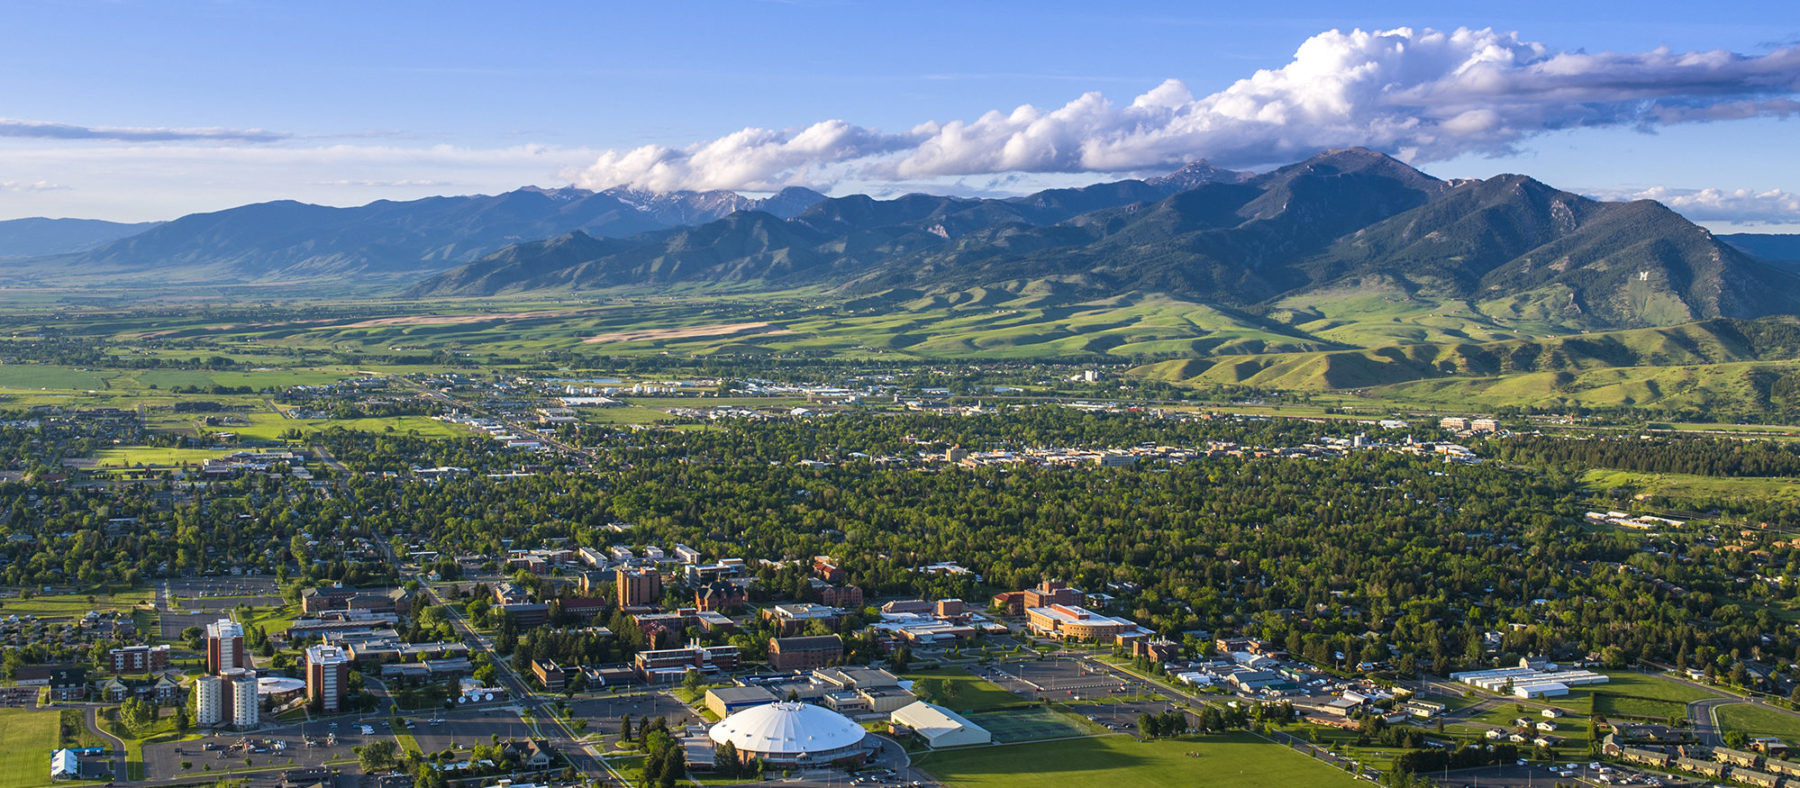
\includegraphics[width=5in,height=\textheight]{images/msu-campus.jpg}}
\usepackage{etoolbox}
\makeatletter
\providecommand{\subtitle}[1]{% add subtitle to \maketitle
  \apptocmd{\@title}{\par {\large #1 \par}}{}{}
}
\makeatother
\subtitle{Fall 2022\\
Montana State University}
\author{Melinda Yager\\
Jade Schmidt\\
Stacey Hancock}
\date{}

\begin{document}
\maketitle

\newpage
\thispagestyle{empty}

This resource was developed by Melinda Yager, Jade Schmidt, and Stacey Hancock in 2021 to accompany the online textbook: Carnegie, N., Hancock, S., Meyer, E., Schmidt, J., and Yager, M. (2021). \emph{Montana State Introductory Statistics with R}. Montana State University. \url{https://mtstateintrostats.github.io/IntroStatTextbook/}.

This resource is released under a \href{https://creativecommons.org/licenses/by-nc-sa/4.0/}{Creative Commons BY-NC-SA 4.0} license unless otherwise noted.

\setcounter{tocdepth}{1}
\addtocontents{toc}{\protect\thispagestyle{empty}}
\tableofcontents
\thispagestyle{empty}

\newpage
\setcounter{page}{1}

\hypertarget{preface}{%
\chapter*{Preface}\label{preface}}
\addcontentsline{toc}{chapter}{Preface}

This coursepack accompanies the textbook for STAT 216: Introduction to Statistics at Montana State University, which can be found at \url{https://mtstateintrostats.github.io/IntroStatTextbook/}. The syllabus for the course (including the course calendar), data sets, and links to D2L Brightspace, Gradescope, and the MSU RStudio server can be found on the course webpage: \url{https://math.montana.edu/courses/s216/}.
Videos assigned in the course calendar and other notes and review materials are linked in D2L.

Each of the activities in this workbook is designed to target specific learning outcomes of the course, giving you practice with important statistical concepts in a group setting with instructor guidance. In addition to the in-class activities for the course, the coursepack includes reading guides to aid in taking notes while you complete the required readings and videos. Bring this workbook with you to class each class period, and take notes in the workbook as you would your own notes. A well-written completed workbook will provide an optimal study guide for exams!

The activities and labs in this coursepack will be completed during class time. Parts of each lab will be turned in on Gradescope. To aid in your understanding, read through the introduction for each activity before attending class each day.

STAT 216 is a 3-credit in-person course. In our experience, it takes six to nine hours per week outside of class to achieve a good grade in this class. By ``good'' we mean at least a C because a grade of D or below does not count toward fulfilling degree requirements. Many of you set your goals higher than just getting a C, and we fully support that. You need roughly nine hours per week to review past activities, read feedback on previous assignments, complete current assignments, and prepare for the next day's class. A typical week in the life of a STAT 216 student looks like:

\begin{itemize}
\tightlist
\item
  \emph{Prior to class meeting}:

  \begin{itemize}
  \tightlist
  \item
    Read assigned sections of the textbook, using the provided reading guides to take notes on the material.
  \item
    Watch assigned videos on that week's content, pausing to take notes and answer video quiz questions.
  \item
    Read through the introduction to the day's in-class activity
  \item
    Read through the week's homework assignment and note any questions you may have on the content.
  \end{itemize}
\item
  \emph{During class meeting}:

  \begin{itemize}
  \tightlist
  \item
    Work through the in-class activity or weekly lab with your classmates and instructor, taking detailed notes on your answers to each question in the activity.
  \end{itemize}
\item
  \emph{After class meeting}:

  \begin{itemize}
  \tightlist
  \item
    Complete any parts of the activity you did not complete in class.
  \item
    Review the activity solutions in the Math and Stat Center, and take notes on key points.
  \item
    Finish watching any remaining assigned videos or readings for the week.
  \item
    Complete the week's homework assignment.
  \end{itemize}
\end{itemize}

\nocite{*}

\hypertarget{fall-2022-calendar-of-in-class-activities}{%
\chapter*{Fall 2022 Calendar of In-Class Activities}\label{fall-2022-calendar-of-in-class-activities}}
\addcontentsline{toc}{chapter}{Fall 2022 Calendar of In-Class Activities}

This calendar only lists the in-class activities, RStudio labs and exams each week. For required readings and videos as well as due dates for assignments, refer to the calendar at:\\
\url{https://mtstateintrostats.github.io/Syllabus/\#Course_calendar}

\begin{longtable}{|l|l|l|l|p{.55\textwidth}|}
\hline
\textbf{Week}& \textbf{Day}& \textbf{Date}& \textbf{Activity} \\ \hline
\endhead

1& W& 8/24& Syllabus Review \\*
1& F& 8/26& Intro to Data \\ \hline
2& M& 8/29& American Indian Address Part A \\*
2& W& 8/31& American Indian Address Part B \\* 
2& F& 9/2& Week 2 Lab \\ \hline
3& M& 9/5& (\textit{No class}) \\*
3& W& 9/7& Myopia and Nightlights \\*
3& F& 9/9& Week 3 Lab \\ \hline
4& M& 9/12& Movie Profits --- Linear Regression \\*
4& W& 9/14& Movie Profits --- Correlation \\*
4& F& 9/16& Week 4 Lab \\ \hline
5& M& 9/19& Exam 1 Review \\*
5& W& 9/21& Group Midterm Exam 1 \\*    
5& F& 9/23& Midterm Exam 1 \\ \hline
6& M& 9/26& Helper Hinderer --- Simulation HT \\*
6& W& 9/28& Helper Hinderer --- Simulation HT continued \\* 
6& F& 9/30& Week 6 Lab \\ \hline
7& M& 10/3& Handedness of Male Boxers --- Theory HT \\*
7& W& 10/5&  Handedness of Male Boxers --- Theory CI\\*
7& F& 10/7& Week 7 Lab \\ \hline
8& M& 10/10& Good Samaritan --- Simulation HT \\*
8& W& 10/12& Good Samaritan --- Simulation CI \\*   
8& F& 10/14& Week 8 Lab \\ \hline
9& M& 10/17& Helmet Use and Head Injuries --- Theory HT \\*
9& W& 10/19& Helmet Use and Head Injuries --- Theory CI \\* 
9& F& 10/21& Week 9 Lab \\ \hline
10& M& 10/24& Exam 2 Review \\*
10& W& 10/26& Group Midterm Exam 2 \\*
10& F& 10/28& Midterm Exam 2\\ \hline
11& M& 10/31& COVID and Air Pollution \\*
11& W& 11/2& Color Interference \\* 
11& F& 11/4& Week 11 Lab \\ \hline
12& M& 11/7& Does Behavior Impact Performance? \\*
12& W& 11/9& Week 12 Lab \\*
12& F& 11/11& (\textit{No class}) \\ \hline
13& M& 11/14& Diving Penguins  \\*
13& W& 11/16& Golf Driving Distances \\*
13& F& 11/18& Week 13 Lab \\ \hline
Holiday& M--F& 11/21--11/25& \textbf{No Class --- Fall Break} \\ \hline
14& M& 11/28& What's the probability? \\*
14& W& 11/30& Relative Risk \\*
14& F& 12/2& Week 14 Lab \\ \hline
15& M& 12/5& Final Exam Review \\*
15& W& 12/7& Final Group Exam Part 1 \\*
15& F& 12/9& Final Group Exam Part 2 \\ \hline
Finals& Tuesday & 12/13 6 - 7:50 pm & Common Final Exam \\
&  &  & See \url{www.montana.edu/registrar/Schedules.html} \\ \hline

\end{longtable}

\nocite{*}

\hypertarget{basics-of-data}{%
\chapter{Basics of Data}\label{basics-of-data}}

\hypertarget{week-1-reading-guide-basics-of-data}{%
\section{Week 1 Reading Guide: Basics of Data}\label{week-1-reading-guide-basics-of-data}}

\hypertarget{sections-1.1-case-study-and-1.2-data-basics}{%
\subsection*{Sections 1.1 (Case study) and 1.2 (Data basics)}\label{sections-1.1-case-study-and-1.2-data-basics}}
\addcontentsline{toc}{subsection}{Sections 1.1 (Case study) and 1.2 (Data basics)}

\textbf{Videos}

\begin{itemize}
\tightlist
\item
  Stat 216 Course\_Tour
\item
  Instructor bio
\item
  1.2.1and1.2.2
\item
  1.2.3to1.2.5
\end{itemize}

\setstretch{1.25}

\hypertarget{vocabulary}{%
\subsubsection*{Vocabulary}\label{vocabulary}}
\addcontentsline{toc}{subsubsection}{Vocabulary}

Data:
\rgs

Sample size:
\rgs

Case/Observational unit:
\rgs

Variable:
\rgs

\rgi Quantitative variable:
\rgs

\rgi Discrete variables:
\rgs

\rgi \rgi Examples of discrete variables using the \texttt{County} data:
\rgs

\rgi Continuous variables:
\rgs

\rgi \rgi Examples of continuous variables using the \texttt{County} data:
\rgs

Example of a number which is NOT a numerical (quantitative) variable:
\rgs

\newpage

Categorical variable:
\rgs

\rgi Ordinal variable:
\rgs

\rgi \rgi Example of an ordinal variable using the \texttt{County} data:
\rgs

\rgi Nominal variable:
\rgs

\rgi \rgi Examples of nominal variables using the \texttt{County} data:

\rgs

\textbf{Note: Ordinal and nominal variables will be treated the same in this course. We recommend taking more statistics courses in the future to learn better methods of analysis for ordinal variables.}

Data frame:
\rgs

Summary statistics:
\rgs

Scatterplot:
\rgs

\rgi Each point represents:

\rgi Positive association:

\rgi Negative association:

Associated or Dependent variables:
\rgs

Independent variables:
\rgs

Explanatory variable:
\rgs

Response variable:
\rgs

Observational study:
\rgs

Randomized Experiment:
\rgs

Placebo:
\rgs

\newpage

\hypertarget{notes}{%
\subsubsection*{Notes}\label{notes}}
\addcontentsline{toc}{subsubsection}{Notes}

Big Idea: Variability is inevitable! We would not expect to get \emph{exactly} 50 heads in 100 coin flips. The statistical question then is whether any differences found in data are due to random variability, or if something else is going on.

\begin{quote}
The larger the difference, the \textbf{less we believe the difference was due to chance.}
\end{quote}

In a data frame, rows correspond to \_\_\_\_\_\_\_\_\_\_\_\_\_\_\_\_\_\_\_

and columns correspond to \_\_\_\_\_\_\_\_\_\_\_\_\_\_\_\_\_\_.

How many types of variables are discussed? Explain the differences between them and give an example of each.
\rgs
\rgs

True or False: A pair of variables can be both associated AND independent.\\
True or False: Given a pair of variables, one will always be the explanatory variable and one the response variable.\\
True or False: If a study does have an explanatory and a response variable, that means changes in the explanatory variable must \textbf{cause} changes in the response variable.

True or False: Observational studies can show a naturally occurring association between variables.

\hypertarget{example-section-1.1-case-study-using-stents-to-prevent-strokes}{%
\subsubsection*{Example (Section 1.1 --- Case study: Using stents to prevent strokes)}\label{example-section-1.1-case-study-using-stents-to-prevent-strokes}}
\addcontentsline{toc}{subsubsection}{Example (Section 1.1 --- Case study: Using stents to prevent strokes)}

\begin{enumerate}
\def\labelenumi{\arabic{enumi}.}
\item
  What is the principle question the researchers hope to answer? (We call this the \textbf{research question}.)
  \rgs
  \rgs
\item
  When creating two groups to compare, do the groups have to be the same size (same number of people in each)?
  \rgs
  \rgs
\item
  What are the cases or observational units in this study?
  \rgs
  \rgs
\item
  Is there a clear explanatory and response variable? If so, name the variable in each role and determine the type of variable (categorical or quantitative).
  \rgs
  \rgs
\item
  What is the purpose of the control group?
  \rgs
  \rgs
\item
  Is this an example of an observational study or a randomized experiment? How do you know?
  \rgs
  \rgs
\end{enumerate}

\newpage

\begin{enumerate}
\def\labelenumi{\arabic{enumi}.}
\setcounter{enumi}{6}
\item
  Consider Tables 1.1 and 1.2. Which table is more helpful in answering the research question? Justify your answer.
  \rgs
  \rgs
\item
  Describe in words what is shown in Figure 1.2. Specifically, compare the proportion of patients who had a stroke between the treatment and control groups after 30 days as well as after 365 days.
  \rgs
  \rgs
\item
  Given the notion that the larger the difference between the two groups (for a given sample size), the less believable it is that the difference was due to chance, which measurement period (30 days or 365 days) provide stronger evidence that there is an association between stents and strokes, or that the differences are not due to random chance?
  \rgs
  \rgs
\item
  This study reported finding evidence that stents \emph{increase} the risk of stroke. Does this conclusion apply to all patients and all stents?
  \rgs
  \rgs
\item
  This study reported finding evidence that stents \emph{increase} the risk of stroke. This conclusion implies a causal link between stents and an increased risk of stroke. Is that conclusion valid? Justify your answer.
  \rgs
  \rgs
\end{enumerate}

\hypertarget{section-2.1-sampling-principles-and-strategies}{%
\subsection*{Section 2.1 (Sampling principles and strategies)}\label{section-2.1-sampling-principles-and-strategies}}
\addcontentsline{toc}{subsection}{Section 2.1 (Sampling principles and strategies)}

\textbf{Videos}

\begin{itemize}
\tightlist
\item
  2.1
\end{itemize}

\setstretch{1.25}

\hypertarget{vocabulary-1}{%
\subsubsection*{Vocabulary}\label{vocabulary-1}}
\addcontentsline{toc}{subsubsection}{Vocabulary}

(Target) Population:
\rgs

Sample:
\rgs

Statistic:
\rgs

Parameter:
\rgs

Anecdotal evidence:
\rgs

\newpage

Bias:
\rgs

\rgi Selection bias:
\rgs

\rgi Non-response bias:
\rgs

\rgi Response bias:
\rgs

Convenience sample:
\rgs

Simple Random Sample:
\rgs

Non-response rate:
\rgs

Representative:
\rgs

\hypertarget{notes-1}{%
\subsubsection*{Notes}\label{notes-1}}
\addcontentsline{toc}{subsubsection}{Notes}

Ideally, how should we sample cases from our target population? What sampling method should be used?
\rgs

\hypertarget{notes-on-types-of-sampling-bias}{%
\paragraph*{Notes on types of sampling bias}\label{notes-on-types-of-sampling-bias}}
\addcontentsline{toc}{paragraph}{Notes on types of sampling bias}

\begin{itemize}
\item
  Someone must first be \emph{chosen} to be in a study and refuse to participate in order to have \textbf{non-response bias}.
\item
  There must be a valid reason for someone to lie or be untruthful to justify saying \textbf{response bias} is present. Yes, anyone could lie at any time to any question. Response bias is when those lies are \emph{predictable and systematic} based on outside influences.
  \rgs
\end{itemize}

True or False: Convenience sampling tends to result in non-response bias.

True or False: Volunteer sampling tends to result in response bias.

True or False: Random sampling helps to resolve selection bias, but has no impact on non-response or response bias.

\newpage

\hypertarget{activity-1-intro-to-data}{%
\section{Activity 1: Intro to Data}\label{activity-1-intro-to-data}}

\setstretch{1}

\hypertarget{learning-outcomes}{%
\subsection{Learning outcomes}\label{learning-outcomes}}

\begin{itemize}
\item
  Identify observational units, variables, and variable types in a statistical study.
\item
  Identify biased sampling methods.
\end{itemize}

\hypertarget{terminology-review}{%
\subsection{Terminology review}\label{terminology-review}}

Statistics is the study of how best to collect, analyze, and draw conclusions from data. Today in class you will be introduced to the following terms:

\begin{itemize}
\item
  Observational units or cases
\item
  Variables: categorical or quantitative
\item
  Types of sampling bias
\end{itemize}

For more on these concepts, read Chapter 1 and Section 2.1 in the textbook.

\hypertarget{general-information-on-labs}{%
\subsection{General information on labs}\label{general-information-on-labs}}

On Friday of each week you will complete a lab. Questions are selected from each lab to be turned in on Gradescope. The questions to be submitted on Gradescope are bolded in the lab. As you work through the lab have the Gradescope lab assignment open so that you can answer those questions as you go. Today's activity is Lab 0 in Gradescope for practice submitting as a group.

\hypertarget{steps-of-the-statistical-investigation-process}{%
\subsubsection*{Steps of the statistical investigation process}\label{steps-of-the-statistical-investigation-process}}
\addcontentsline{toc}{subsubsection}{Steps of the statistical investigation process}

As we move through the semester we will work through the six steps of the statistical investigation process.

\begin{enumerate}
\def\labelenumi{\arabic{enumi}.}
\item
  Ask a research question.
\item
  Design a study and collect data.
\item
  Summarize and visualize the data. \emph{Weeks 3--4}
\item
  Use statistical analysis methods to draw inferences from the data. \emph{Weeks 6--13}
\item
  Communicate the results and answer the research question. \emph{Weeks 6--13}
\item
  Revisit and look forward.
\end{enumerate}

Today we will focus on the first two steps.

\textbf{Step 1}: The first step of any statistical investigation is to \emph{ask a research question}. As stated in the textbook, ``with the rise of data science, however, we might not start with a research question, and instead start with a data set.'' Today we will create a data set by collecting responses on students in class.

\textbf{Step 2}: To answer any research question, we must \emph{design a study and collect data}. Our study will consist of answers from each student. Your responses will become our observed data that we will explore.

\textbf{Observational units} or \textbf{cases} are the subjects data are collected on. In a spreadsheet of the data set, each row will represent a single observational unit.

\begin{enumerate}
\def\labelenumi{\arabic{enumi}.}
\tightlist
\item
  \textbf{What are the observational units or cases for today's study? }
\end{enumerate}

\vspace{0.2in}

\begin{enumerate}
\def\labelenumi{\arabic{enumi}.}
\setcounter{enumi}{1}
\tightlist
\item
  How many students are in class today? This is the \textbf{sample size}.
\end{enumerate}

\vspace{0.2in}

A \textbf{variable} is information collected or measured on each observational unit or case. Each column in a data set will represent a different variable.

One person from each group at each table, open the Google sheet linked in D2L and fill in the responses for the following questions for each group member. When creating a data set for use in R it is important to use single words or an underscore between words. Each outcome must be written the same way each time. Make sure to use all lowercase letters to create this data set to have consistency between responses. Do not give units of measure with the numerical values for the length of forearm. For \texttt{Residency} use in\_state or out\_state as the two outcomes.

\begin{itemize}
\tightlist
\item
  Major: what is your declared major?
\item
  Residency: do you have in-state or out-of-state residency?
\item
  Forearm\_Length: what is the length of your forearm in inches from the end of your elbow to the end of your index finger?
\item
  Num\_Credits: how many credits are you taking this semester?
\end{itemize}

We will look at two types of variables: \textbf{quantitative} and \textbf{categorical} (see Figure \ref{fig:types-of-variables}).

Quantitative variables are numerical measurements that can be discrete (whole, non-negative numbers) or continuous (any value within an interval). The number of pets one owns would be a discrete variable as you can not have a partial pet. GPA would be a continuous variable ranging from 0 to 4.0.

The outcome of a categorical variable is a group or category such as eye color, state of residency, or whether or not a student lives on campus. Categorical variables with a natural ordering are considered ordinal variables while those without a natural ordering are considered nominal variables. All categorical variables will be treated as nominal for analysis in this course.

\begin{figure}

{\centering 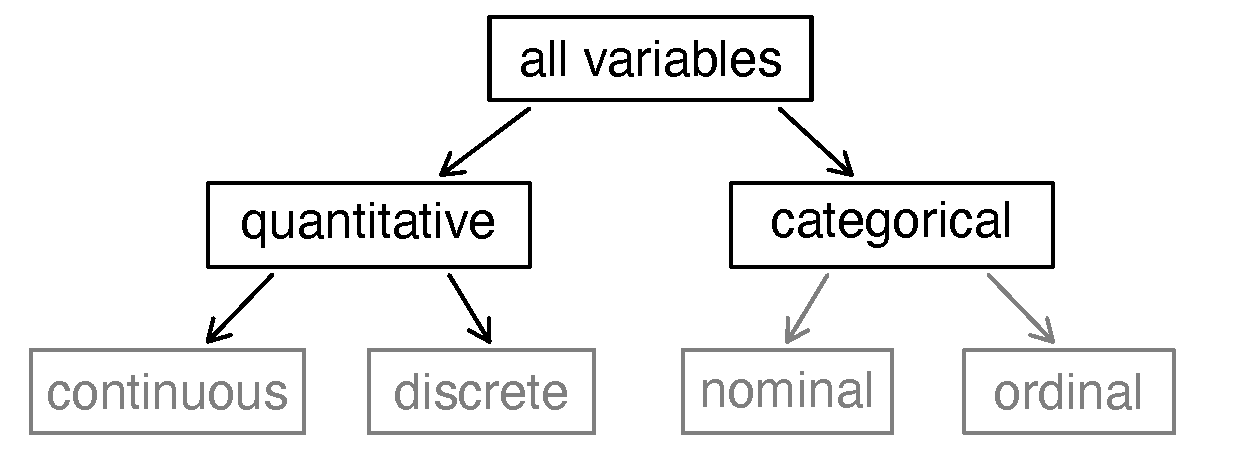
\includegraphics[width=0.5\linewidth]{images/variables} 

}

\caption{Types of variables.}\label{fig:types-of-variables}
\end{figure}

\newpage

\begin{enumerate}
\def\labelenumi{\arabic{enumi}.}
\setcounter{enumi}{2}
\tightlist
\item
  For each column of data, fill in the following table to write out the variable we are collecting on each observational unit in this study and the type of each variable.
\end{enumerate}

\begin{center}
\begin{tabular}{|l|p{2in}|p{2in}|} \hline
Column & Variable & Type of Variable  \\ \hline
Major & & \\ 
& & \\ \hline
Residency & & \\ 
& & \\ \hline
Forearm Length & & \\ 
& & \\ \hline
Num Credits & & \\ 
& & \\ \hline
\end{tabular}
\end{center}

In the next few weeks we will look at how to summarize data both numerically and graphically. For now we will focus on sampling methods and the type of sampling bias that may be present.

\begin{itemize}
\item
  Sampling bias: a part of the target population is not included or underrepresented in the sample
\item
  Non-response or non-participation bias: part of the already selected population does not respond or chooses not to participate
\item
  Response bias: survey participant gives an untruthful or misleading response
\end{itemize}

To help determine the type of bias present, it is helpful to think about the observational units, the sample and the target population represented by the problem. The \textbf{target population} is the group of cases that makes up the population the researcher is interested in. If sampling bias is present, than the sample taken will not be representative of the actual target population. In these next questions, identify the target population, the sample selected, the variable collected and its type (categorical or quantitative), and the type of bias present.

\begin{enumerate}
\def\labelenumi{\arabic{enumi}.}
\setcounter{enumi}{3}
\item
  \textbf{To determine if the proportion of out-of-state undergraduate students at Montana State University has increased in the last 10 years, a statistics instructor sent an email survey to 500 randomly selected current undergraduate students. One of the questions on the survey asked whether they had in-state or out-of-state residency. She only received 378 responses.}
  \vspace{0.25in}

  Observational units or cases:
  \vspace{0.3in}

  Target population:
  \vspace{0.3in}

  Sample size:
  \vspace{0.3in}

  Sample taken:
  \vspace{0.3in}

  Variable:
  \vspace{0.3in}

  Type of Variable: \hspace{1mm} categorical \hspace{0.2in} quantitative
  \vspace{1mm}

  Type(s) of bias:
  \vspace{0.3in}
\item
  A television station is interested in predicting whether or not a local referendum to legalize marijuana for adult use will pass. It asks its viewers to phone in and indicate whether they are in favor or opposed to the referendum. Of the 2241 viewers who phoned in, forty-five percent were opposed to legalizing marijuana.
  \vspace{0.1in}

  Observational units or cases:
  \vspace{0.3in}

  Target population:
  \vspace{0.3in}

  Sample size:
  \vspace{0.3in}

  Sample taken:
  \vspace{0.3in}

  Variable:
  \vspace{0.3in}

  Type of Variable: \hspace{1mm} categorical \hspace{0.2in} quantitative
  \vspace{1mm}

  Type(s) of bias:
  \vspace{0.3in}
\item
  To gauge the interest in a new swimming pool, a local organization stood outside of the Bogart Pool in Bozeman, MT, during open hours. One of the questions they asked was, ``Since the Bogart Pool is in such bad repair, don't you agree that the city should fund a new pool?''
  \vspace{0.1in}

  Observational units or cases:
  \vspace{0.3in}

  Target population:
  \vspace{0.3in}

  Sample size:
  \vspace{0.3in}

  Sample taken:
  \vspace{0.3in}

  Variable:
  \vspace{0.3in}

  Type of Variable: \hspace{1mm} categorical \hspace{0.2in} quantitative
  \vspace{1mm}

  Type(s) of bias:
  \vspace{0.3in}
\end{enumerate}

\newpage

\begin{enumerate}
\def\labelenumi{\arabic{enumi}.}
\setcounter{enumi}{6}
\tightlist
\item
  \textbf{The Bozeman school district was interested in surveying parents of students about their opinions on returning to in-person classes following the COVID-19 pandemic. They divided the school district into 10 divisions based on location and randomly surveyed 20 households within each division. Explain why selection bias would be present in this study design.}
  \vspace{1in}
\end{enumerate}

\hypertarget{take-home-messages}{%
\subsection{Take-home messages}\label{take-home-messages}}

\begin{enumerate}
\def\labelenumi{\arabic{enumi}.}
\item
  When creating a data set, each row will represent a single observational unit or case. Each column represents a variable collected. It is important to write each variable as a single word or use an underscore between words.
\item
  There are two types of variables: categorical (groups) and quantitative (numerical measures).
\item
  There are three types of bias to be aware of when designing a sampling method: selection bias, non-response bias, and response bias.
\end{enumerate}

\hypertarget{additional-notes}{%
\subsection{Additional notes}\label{additional-notes}}

Use this space to summarize your thoughts and take additional notes on today's activity and material covered, and to write down the names and contact information of your teammates.

\newpage

\hypertarget{study-design}{%
\chapter{Study Design}\label{study-design}}

\hypertarget{week-2-reading-guide-sampling-experimental-design-and-scope-of-inference}{%
\section{Week 2 Reading Guide: Sampling, Experimental Design, and Scope of Inference}\label{week-2-reading-guide-sampling-experimental-design-and-scope-of-inference}}

\hypertarget{sections-2.2-observational-studies-2.3-experiments-and-2.4-scope-of-inference}{%
\subsection*{Sections 2.2 (Observational studies), 2.3 (Experiments), and 2.4 (Scope of inference)}\label{sections-2.2-observational-studies-2.3-experiments-and-2.4-scope-of-inference}}
\addcontentsline{toc}{subsection}{Sections 2.2 (Observational studies), 2.3 (Experiments), and 2.4 (Scope of inference)}

\setstretch{1}

\textbf{Videos}

\begin{itemize}
\tightlist
\item
  2.2to2.4
\end{itemize}

\setstretch{1.25}

\hypertarget{reminders-from-section-1.2}{%
\subsubsection*{Reminders from Section 1.2}\label{reminders-from-section-1.2}}
\addcontentsline{toc}{subsubsection}{Reminders from Section 1.2}

\textbf{Explanatory variable}: The variable researchers think \emph{may be} affecting the other variable. What the researchers control/assign in an experiment. If comparing groups, the explanatory variable puts the observational units into groups.

\textbf{Response variable}: The variable researchers think \emph{may be} influenced by the other variable. This variable is always observed, never controlled or assigned.

\hypertarget{vocabulary-2}{%
\subsubsection*{Vocabulary}\label{vocabulary-2}}
\addcontentsline{toc}{subsubsection}{Vocabulary}

Observational study:
\rgs

\rgi Observational data:
\rgs

\rgi Prospective study:
\rgs

\rgi Retrospective study:
\rgs

Confounding variable:
\rgs

Experiment:
\rgs

\rgi Randomized experiment:
\rgs

\rgi Blocking:
\rgs

\rgi Treatment group:
\rgs

\rgi Control group:
\rgs

\rgi Blinding:
\rgs

\rgi Placebo:
\rgs

\rgi Placebo effect:
\rgs

Scope of inference:
\rgs

\rgi Generalizability:
\rgs

\rgi Causation:
\rgs

\hypertarget{notes-2}{%
\subsubsection*{Notes}\label{notes-2}}
\addcontentsline{toc}{subsubsection}{Notes}

What are the four principles of a well-designed randomized experiment?\\
\rgs
\rgs
\rgs

Fill in the appropriate scope of inference for each study design.

\begin{center}
\begin{tabular}{|p{2in}|p{2in}|p{2in}|}
\hline
 & \multicolumn{2}{|c|}{\textbf{Study Type}} \\ \hline
 \textbf{Selection of Cases} & Randomized experiment & Observational study \\ \hline
 Random sample && \\ 
 (and no other sampling bias) & & \\ 
  & & \\
   & & \\ \hline
   Non-random sample && \\ 
   (or other sampling bias) & & \\ 
  & & \\
   & & \\ \hline
\end{tabular}
\end{center}

\rgs

True or False: Observational studies can show an association between two variables, but cannot determine a causal relationship.

True or False: In order for an experiment to be valid, a placebo must be used.

True or False: If random sampling of the target population is used, and no other types of bias are suspected, results from the sample can be generalized to the entire target population.

True or False: If random sampling of the target population is used, and no other types of bias are suspected, results from the sample can be inferred as a causal relationship between the explanatory and response variables.

\newpage

\hypertarget{activity-2a-american-indian-address}{%
\section{Activity 2A: American Indian Address}\label{activity-2a-american-indian-address}}

\setstretch{1}

\hypertarget{learning-outcomes-1}{%
\subsection{Learning outcomes}\label{learning-outcomes-1}}

\begin{itemize}
\item
  Explain why a sampling method is unbiased or biased.
\item
  Identify biased sampling methods.
\item
  Explain the purpose of random selection and its effect on scope of inference.
\end{itemize}

\hypertarget{terminology-review-1}{%
\subsection{Terminology review}\label{terminology-review-1}}

In today's activity, we will examine unbiased and biased methods of sampling. Some terms covered in this activity are:

\begin{itemize}
\item
  Random sample
\item
  Unbiased vs biased methods of selection
\item
  Generalization
\end{itemize}

To review these concepts, see Section 2.1 in the textbook.

\hypertarget{american-indian-address}{%
\subsection{American Indian Address}\label{american-indian-address}}

For this activity, you will read a speech given by Jim Becenti, a member of the Navajo American Indian tribe, who spoke about the employment problems his people faced at an Office of Indian Affairs meeting in Phoenix, Arizona, on January 30, 1947 (Moquin and Van Doren 1973). His speech is below:

\textbf{It is hard for us to go outside the reservation where we meet strangers. I have been off the reservation ever since I was sixteen. Today I am sorry I quit the Santa Fe {[}Railroad{]}. I worked for them in 1912-13. You are enjoying life, liberty, and happiness on the soil the American Indian had, so it is your responsibility to give us a hand, brother. Take us out of distress. I have never been to vocational school. I have very little education. I look at the white man who is a skilled laborer. When I was a young man I worked for a man in Gallup as a carpenter's helper. He treated me as his own brother. I used his tools. Then he took his tools and gave me a list of tools I should buy and I started carpentering just from what I had seen. We have no alphabetical language.}

\textbf{We see things with our eyes and can always remember it. I urge that we help my people to progress in skilled labor as well as common labor. The hope of my people is to change our ways and means in certain directions, so they can help you someday as taxpayers. If not, as you are going now, you will be burdened the rest of your life. The hope of my people is that you will continue to help so that we will be all over the United States and have a hand with you, and give us a brotherly hand so we will be happy as you are. Our reservation is awful small. We did not know the capacity of the range until the white man come and say ``you raise too much sheep, got to go somewhere else,'' resulting in reduction to a skeleton where the Indians can't make a living on it. For eighty years we have been confused by the general public, and what is the condition of the Navajo today? Starvation! We are starving for education. Education is the main thing and the only thing that is going to make us able to compete with you great men here talking to us.}

\hypertarget{by-eye-selection}{%
\subsubsection*{By eye selection}\label{by-eye-selection}}
\addcontentsline{toc}{subsubsection}{By eye selection}

\begin{enumerate}
\def\labelenumi{\arabic{enumi}.}
\tightlist
\item
  Circle ten words in Jim Becenti's speech which are a representative sample of the length of words in the entire text. Describe your method for selecting this sample.
\end{enumerate}

\vspace{0.3in}

\begin{enumerate}
\def\labelenumi{\arabic{enumi}.}
\setcounter{enumi}{1}
\tightlist
\item
  Fill in the table below with your selected words from the previous question and the length of each word (number of letters/digits in the word):
  \vspace{1mm}
\end{enumerate}

\begin{center}
\begin{tabular}{|l|p{3in}|p{1in}|} \hline
Observation & Word & Length  \\ \hline
1 & & \\ 
& & \\ \hline
2 & & \\ 
& & \\ \hline
3 & & \\ 
& & \\ \hline
4 & & \\ 
& & \\ \hline
5 & & \\ 
& & \\ \hline
6 & & \\ 
& & \\ \hline
7 & & \\
& & \\ \hline
8 & & \\ 
& & \\ \hline
9 & & \\ 
& & \\ \hline
10 & & \\ 
& & \\ \hline
\end{tabular}
\end{center}

\begin{enumerate}
\def\labelenumi{\arabic{enumi}.}
\setcounter{enumi}{2}
\item
  Calculate the mean (average) word length in your selected sample. Is this value a parameter or a statistic?\\
  \vspace{0.3in}
\item
  Report your mean word length to your instructor. Your instructor will guide the class in creating a visualization of the distribution of results generated by your class. Draw a picture of the plot here. Include a descriptive \(x\)-axis label.
  \vspace{1.5in}
\item
  Based on the plot of sample mean word lengths in question 4, what is your best guess for the average word length of the population of all 359 words in the speech?
  \vspace{0.3in}
\item
  The true mean word length of the population of all 359 words in the speech is 3.95 letters. Is this value a parameter or a statistic?\\
  \vspace{0.2in}

  Where does the value of 3.95 fall in the plot created in question 4? Near the center of the distribution? In the tails of the distribution?
  \vspace{0.3in}
\item
  If the class samples were truly representative of the population of words, what proportion of sample means would you expect to be below 3.95?
  \vspace{0.5in}
\item
  Using the graph created in question 4, estimate the proportion of students' computed sample means that were lower than the true mean of 3.95 letters?
  \vspace{0.5in}
\item
  Based on your answers to questions 7 and 8, would you say the sampling method used by the class is biased or unbiased? Justify your answer.\\
  \vspace{0.5in}
\item
  If the sampling method is biased, what type of sampling bias (selection, response, non-response) is present? What is the direction of the bias, i.e., does the method tend to overestimate or underestimate the population mean word length?
  \vspace{0.5in}
\item
  Should we use results from our by eye samples to make a statement about the word length in the population of words in Becenti's address? Why or why not?
  \vspace{1in}
\end{enumerate}

\hypertarget{take-home-messages-1}{%
\subsection{Take-home messages}\label{take-home-messages-1}}

\begin{enumerate}
\def\labelenumi{\arabic{enumi}.}
\item
  When we use a biased method of selection, we will over or underestimate the parameter.
\item
  To see if a method is biased, we compare the distribution of the estimates to the true value. We want our estimate to be on target or unbiased. When using unbiased methods of selection, the mean of the distribution matches or is very similar to our true parameter.
\item
  If the sampling method is biased, inferences made about the population based on a sample estimate will not be valid.
\end{enumerate}

\hypertarget{additional-notes-1}{%
\subsection{Additional notes}\label{additional-notes-1}}

Use this space to summarize your thoughts and take additional notes on today's activity and material covered.

\newpage

\hypertarget{activity-2b-american-indian-address-continued}{%
\section{Activity 2B: American Indian Address (continued)}\label{activity-2b-american-indian-address-continued}}

\setstretch{1}

\hypertarget{learning-outcomes-2}{%
\subsection{Learning outcomes}\label{learning-outcomes-2}}

\begin{itemize}
\item
  Explain the purpose of random selection and its effect on scope of inference.
\item
  Select a simple random sample from a finite population using a random number generator.
\item
  Explain why a sampling method is unbiased or biased.
\item
  Explain the effect of sample size on sampling variability.
\end{itemize}

\hypertarget{terminology-review-2}{%
\subsection{Terminology review}\label{terminology-review-2}}

In today's activity, we will examine unbiased and biased methods of sampling. Some terms covered in this activity are:

\begin{itemize}
\item
  Random sample
\item
  Unbiased vs biased methods of selection
\item
  Generalization
\end{itemize}

To review these concepts, see Section 2.1 in the textbook.

\hypertarget{random-selection}{%
\subsubsection*{Random selection}\label{random-selection}}
\addcontentsline{toc}{subsubsection}{Random selection}

Today we will return to the American Indian Address introduced in Activity 2A. Suppose instead of attempting to select a representative sample by eye (which did not work), each student used a random number generator to select a simple random sample of 10 words. A \textbf{simple random sample} relies on a random mechanism to choose a sample, without replacement, from the population, such that every sample of size 10 is equally likely to be chosen.

To use a random number generator to select a simple random sample, you first need a numbered list of all the words in the population, called a \textbf{sampling frame}. You can then generate 10 random numbers from the numbers 1 to 359 (the number of words in the population), and the chosen random numbers correspond to the chosen words in your sample.

\begin{enumerate}
\def\labelenumi{\arabic{enumi}.}
\tightlist
\item
  Use the random number generator at \url{https://istats.shinyapps.io/RandomNumbers/} to select a simple random sample from the population of all 359 words in the speech.
\end{enumerate}

\begin{itemize}
\item
  Set ``Choose Minimum'' to 1 and ``Choose Maximum'' to 359 to represent the 359 words in the population (the sampling frame).
\item
  Set ``How many numbers do you want to generate?'' to 10 and ensure the ``No'' option is selected under ``Sample with Replacement?''
\item
  Click ``Generate''.
\end{itemize}

\newpage

Fill in the table below with the random numbers selected and use the Becenti.csv data file found on D2L to determine each number's corresponding word and word length (number of letters/digits in the word):

\begin{center}
\begin{tabular}{|l|l|p{3in}|p{1in}|} \hline
Observation & Number & Word & Length  \\ \hline
1 & & & \\ 
& & & \\ \hline
2 & & & \\ 
& & & \\ \hline
3 & & & \\ 
& & & \\ \hline
4 & & & \\ 
& & & \\ \hline
5 & & & \\ 
& & & \\ \hline
6 & & & \\ 
& & & \\ \hline
7 & & & \\
& & & \\ \hline
8 & & & \\ 
& & & \\ \hline
9 & & &\\ 
& & & \\ \hline
10 & & & \\ 
& & & \\ \hline
\end{tabular}
\end{center}

``

\begin{enumerate}
\def\labelenumi{\arabic{enumi}.}
\setcounter{enumi}{1}
\item
  Calculate the mean word length in your selected sample in question 1. Is this value a parameter or a statistic?
  \vspace{0.3in}
\item
  Report your mean word length to your instructor. Your instructor will guide the class in creating a visualization of the distribution of results generated by your class. Draw a picture of the plot here. Include a descriptive \(x\)-axis label.
  \vspace{1.7in}
\item
  Where does the value 3.95, the true mean word length, fall in the distribution created in question 3? Near the center of the distribution? In the tails of the distribution?
  \vspace{0.3in}
\end{enumerate}

\newpage

\begin{enumerate}
\def\labelenumi{\arabic{enumi}.}
\setcounter{enumi}{4}
\tightlist
\item
  How does the plot generated in question 3 compare to the plot generated in question 4 from Activity 2A?
\end{enumerate}

\rgi Which features are similar?\\
\vspace{0.4in}

\rgi Which features differ?

\vspace{0.4in}

\rgi Why didn't everyone get the same sample mean?
\vspace{0.4in}

One set of randomly generated sample mean word lengths from a single class may not be large enough to visualize the distribution results. Let's have a computer generate 1,000 sample mean word lengths for us.

\begin{itemize}
\item
  Navigate to the ``One Variable with Sampling'' Rossman/Chance web applet: \url{http://www.rossmanchance.com/applets/2021/sampling/OneSample.html?population=gettysburg}.
\item
  Click ``Clear'' below the text box containing data from the Gettysburg address to delete that data set.
\item
  Download the Becenti.csv file from D2L and open the spreadsheet on your computer.
\item
  Copy and paste the population of word lengths (column C) into the applet from the data set provided making sure to include the header. Click ``Use Data''. Verify that the mean for the data set is 3.953 with a sample size of 359. If these are not the values you got, check with your instructor for help with copying in the data set correctly.
\item
  Click the check-box for ``Show Sampling Options''
\item
  Select 1000 for ``Number of samples'' and select 10 for the ``Sample size''.
\item
  Click ``Draw Samples''.
\end{itemize}

\begin{enumerate}
\def\labelenumi{\arabic{enumi}.}
\setcounter{enumi}{5}
\item
  The plot labeled ``Statistics'' displays the 1,000 randomly generated sample mean word lengths. Sketch this plot below. Include a descriptive \(x\)-axis label and be sure to write down the provided mean and SD (standard deviation) of the distribution.
  \vspace{1.5in}
\item
  What is the center value of the distribution created in question 6?
  \vspace{0.3in}
\end{enumerate}

\newpage

\begin{enumerate}
\def\labelenumi{\arabic{enumi}.}
\setcounter{enumi}{7}
\item
  Explain why the sampling method of using a random number generator to generate a sample is a ``better'' method than choosing 10 words ``by eye''.
  \vspace{0.8in}
\item
  Is random selection an unbiased method of selection? Explain your answer. Be sure to reference your plot from question 6.
  \vspace{0.5in}
\end{enumerate}

\hypertarget{effect-of-sample-size}{%
\subsection*{Effect of sample size}\label{effect-of-sample-size}}
\addcontentsline{toc}{subsection}{Effect of sample size}

We will now consider the impact of sample size.

\begin{enumerate}
\def\labelenumi{\arabic{enumi}.}
\setcounter{enumi}{9}
\item
  First, consider if each student had selected 20 words, instead of 10, by eye. Do you think this would make the plot from question 4 in Activity 2A centered on 3.95 (the true mean word length)? Explain your answer.
  \vspace{0.4in}
\item
  Now we will select 20 words instead of 10 words at random.
\end{enumerate}

\begin{itemize}
\item
  In the ``One Variable with Sampling'' Rossman/Chance web applet(\url{http://www.rossmanchance.com/applets/2021/sampling/OneSample.html?population=gettysburg}.), change the Sample size to 20.
\item
  Click ``Draw Samples''.
\end{itemize}

The plot labeled ``Statistics'' displays the 1,000 randomly generated sample mean word lengths. Sketch this plot below. Include a descriptive \(x\)-axis label and be sure to write down the provided mean and SD (standard deviation) of the distribution.
\vspace{1.6in}

\begin{enumerate}
\def\labelenumi{\arabic{enumi}.}
\setcounter{enumi}{11}
\tightlist
\item
  Compare the distribution created in question 11 to the one created in question 6.
\end{enumerate}

\rgi Which features are similar?\\
\vspace{0.3in}

\rgi Which features differ?

\vspace{0.3in}

\newpage

\begin{enumerate}
\def\labelenumi{\arabic{enumi}.}
\setcounter{enumi}{12}
\item
  Compare the spreads of the plots in question 11 and in question 6. You should see that in one plot all sample means are closer to the population mean than in the other. Which plot shows this?
  \vspace{0.4in}
\item
  Using the evidence from your simulations, answer the following research questions:
\end{enumerate}

\rgi Does changing the sample size impact whether the sample estimates are unbiased? Explain your answer.
\vspace{0.5in}

\rgi Does changing the sample size impact the variability (spread) of sample estimates? Explain your answer
\vspace{0.5in}

\begin{enumerate}
\def\labelenumi{\arabic{enumi}.}
\setcounter{enumi}{14}
\tightlist
\item
  What is the purpose of random selection of a sample from the population?
\end{enumerate}

\vspace{0.8in}

\hypertarget{take-home-messages-2}{%
\subsection{Take-home messages}\label{take-home-messages-2}}

\begin{enumerate}
\def\labelenumi{\arabic{enumi}.}
\item
  Random selection is an unbiased method of selection.
\item
  To determine if a sampling method is biased or unbiased, we compare the distribution of the estimates to the true value. We want our estimate to be on target or unbiased. When using unbiased methods of selection, the mean of the distribution matches or is very similar to our true parameter.
\item
  Random selection eliminates selection bias. However, random selection will not eliminate response or non-response bias.
\item
  The larger the sample size, the more similar (less variable) the statistics will be from different samples.
\item
  Sample size has no impact on whether a \emph{sampling method} is biased or not. Taking a larger sample using a biased method will still result in a sample that is not representative of the population.
\end{enumerate}

\hypertarget{additional-notes-2}{%
\subsection{Additional notes}\label{additional-notes-2}}

Use this space to summarize your thoughts and take additional notes on today's activity and material covered.

\newpage

\hypertarget{week-2-lab-study-design}{%
\section{Week 2 Lab: Study Design}\label{week-2-lab-study-design}}

\setstretch{1}

\hypertarget{learning-outcomes-3}{%
\subsection{Learning outcomes}\label{learning-outcomes-3}}

\begin{itemize}
\item
  Explain the purpose of random assignment and its effect on scope of inference.
\item
  Identify whether a study design is observational or an experiment.
\item
  Identify confounding variables in observational studies and explain why they are confounding.
\end{itemize}

\hypertarget{terminology-review-3}{%
\subsection{Terminology review}\label{terminology-review-3}}

In this activity, we will examine different study designs, confounding variables, and how to determine the scope of inference for a study. Some terms covered in this activity are:

\begin{itemize}
\item
  Scope of inference
\item
  Explanatory variable
\item
  Response variable
\item
  Confounding variable
\item
  Experiment
\item
  Observational study
\end{itemize}

To review these concepts, see Sections 2.2 through 2.5 in the textbook.

\hypertarget{general-information-labs}{%
\subsection{General information labs}\label{general-information-labs}}

Remember that each Friday you will complete a lab. Questions are selected from each lab to be turned in on Gradescope. The questions to be submitted on Gradescope are bolded in the lab. As you work through the lab have the Gradescope lab assignment open so that you can answer those questions as you go.

\hypertarget{study-design-1}{%
\subsection*{Study design}\label{study-design-1}}
\addcontentsline{toc}{subsection}{Study design}

The two main study designs we will cover are \textbf{observational studies} and \textbf{experiments}. In observational studies, researchers have no influence over which subjects are in each group being compared (though they can control other variables in the study). An experiment is defined by assignment of the treatment groups of the \emph{explanatory variable}, typically via random assignment. In today's activity we will discover the purpose behind random assignment.

For the next exercises, identify the explanatory variable, the response variable, and the study design (observational study or experiment).

\newpage

\begin{enumerate}
\def\labelenumi{\arabic{enumi}.}
\item
  The pharmaceutical company Moderna Therapeutics, working in conjunction with the National Institutes of Health, conducted Phase 3 clinical trials of a vaccine for COVID-19 last fall. US clinical research sites enrolled 30,000 volunteers without COVID-19 to participate. Participants were randomly assigned to receive either the candidate vaccine or a saline placebo. They were then followed to assess whether or not they developed COVID-19. The trial was double-blind, so neither the investigators nor the participants knew who was assigned to which group.
  \vspace{0.1in}

  Explanatory variable:
  \vspace{0.25in}

  Response variable:
  \vspace{0.25in}

  Study design:
  \vspace{0.25in}
\item
  \textbf{In another study, a local health department randomly selected 1000 US adults without COVID-19 to participate in a health survey. Each participant was assessed at the beginning of the study and then followed for one year. They were interested to see which participants elected to receive a vaccination for COVID-19 and whether any participants developed COVID-19.}
  \vspace{0.1in}

  Explanatory variable:
  \vspace{0.25in}

  Response variable:
  \vspace{0.25in}

  Study design:
  \vspace{0.25in}
\end{enumerate}

\hypertarget{atrial-fibrillation}{%
\subsection*{Atrial fibrillation}\label{atrial-fibrillation}}
\addcontentsline{toc}{subsection}{Atrial fibrillation}

Atrial fibrillation is an irregular and often elevated heart rate. In some people, atrial fibrillation will come and go on its own, but others will experience this condition on a permanent basis. When atrial fibrillation is constant, medications are required to stabilize the patient's heart rate and to help prevent blood clots from forming. Pharmaceutical scientists at a large pharmaceutical company believe they have developed a new medication that effectively stabilizes heart rates in people with permanent atrial fibrillation. They set out to conduct a trial study to investigate the new drug. The scientists will need to compare the proportion of patients whose heart rate is stabilized between two groups of subjects, one of whom is given a placebo and the other given the new medication.

\begin{enumerate}
\def\labelenumi{\arabic{enumi}.}
\setcounter{enumi}{2}
\item
  Identify the explanatory and response variable in this trial study.

  Explanatory variable:
  \vspace{0.5in}

  Response variable:
  \vspace{0.5in}
\end{enumerate}

\newpage

Suppose 24 subjects with permanent atrial fibrillation have volunteered to participate in this study:

Self-identified males: Paul, Antonio, Davieon, Chao, Aryan, Jabari, Tong, Andres, John, Liu, Lucas, Rashidi, Shiwoo, Jihoon, Alejandro, Daniel

Self-identified females: An, Nailah, Jasmine, Ka Nong, Keyaina, Mary, Adah, Sassandra

\begin{enumerate}
\def\labelenumi{\arabic{enumi}.}
\setcounter{enumi}{3}
\item
  Is this a simple random sample or a convenience sample? How do you know?
  \vspace{0.5in}
\item
  Based on the sampling method, to what population should the results of this study be generalized?
  \vspace{0.5in}
\item
  One way to separate into two groups would be give all the males the placebo and all the females the new drug. Would this be a reasonable strategy? Explain your answer.
  \vspace{1in}
\item
  Could the scientists fix the problem with the strategy presented in question 6 by creating equal sized groups by putting 4 males and 8 females into the drug group and the remaining 12 males in the placebo group? Explain your answer.
  \vspace{0.5in}
\item
  A third strategy would be to \textbf{block} on sex. In this type of study, the scientists would assign 4 females and 8 males to each group. Using this strategy, what proportion of males is in each group?
  \vspace{0.3in}
\item
  \textbf{Assume the scientists used the strategy in question 8, but they put the four tallest females and eight tallest males into the placebo group and the remaining subjects into the control group. They found that the proportion of patients whose heart rate stabilized is higher in the drug group than the placebo group.}\\
  \vspace{0.1in}

  Could that difference be due to the sex of the subjects? Explain your answer.
  \vspace{0.5in}

  Could it be due to other variables? Explain your answer.
  \newpage
\end{enumerate}

While the strategy presented in question 9 controlled for the sex of the subject, there are more potential \textbf{confounding variables} in the study. A confounding variable is a variable that is \emph{both}

\begin{enumerate}
\def\labelenumi{\arabic{enumi}.}
\tightlist
\item
  associated with the explanatory variable, \emph{and}
\item
  associated with the response variable.
\end{enumerate}

When both these conditions are met, if we observe an association between the explanatory variable and the response variable in the data, we cannot be sure if this association is due to the explanatory variable or the confounding variable---the explanatory and confounding variables are ``confounded.''

\textbf{Random assignment} means that subjects in a study have an equally likely chance of receiving any of the available treatments.

\begin{enumerate}
\def\labelenumi{\arabic{enumi}.}
\setcounter{enumi}{9}
\tightlist
\item
  You will now investigate how randomly assigning subjects impacts a study's scope of inference.
\end{enumerate}

\begin{itemize}
\item
  Navigate to the ``Randomizing Subjects'' applet under the ``Other Applets'' heading at: \url{http://www.rossmanchance.com/ISIapplets.html}. This applet lists the sex and height of each of the 24 subjects. Click ``Show Graphs'' to see a bar chart showing the sex of each subject. Currently, the applet is showing the strategy outlined in question 7.
\item
  Click ``Randomize''.
\end{itemize}

~~~In this random assignment, what proportion of males are in group 1 (the placebo group)?

\vspace{0.1in}

~~~What proportion of males are in group 2 (the drug group)?

\vspace{0.1in}

~~~What is the difference in proportion of males between the two groups (placebo - drug)?

\vspace{0.1in}

\begin{enumerate}
\def\labelenumi{\arabic{enumi}.}
\setcounter{enumi}{10}
\item
  Notice the difference in the two proportions is shown as a dot in the plot at the bottom of the web page. Un-check the box for Animate above ``Randomize'' and click ``Randomize'' again. Did you get the same difference in proportion of males between the placebo and drug groups?
  \vspace{0.25in}
\item
  Change ``Replications'' to 998 (for 1000 total). Click ``Randomize'' again. Sketch the plot of the distribution of difference in proportions from each of the 1000 random assignments here. Be sure to include a descriptive \(x\)-axis label.
  \vspace{1.25in}
\end{enumerate}

\newpage

\begin{enumerate}
\def\labelenumi{\arabic{enumi}.}
\setcounter{enumi}{12}
\item
  \textbf{Does random assignment \emph{always} balance the placebo and drug groups based on the sex of the participants? Does random assignment \emph{tend} to make the placebo and drug groups \emph{roughly} the same with respect to the distribution of sex? Use your plot from question 12 to justify your answers.}
  \vspace{0.5in}
\item
  Change the drop-down menu below Group 2 from ``sex'' to ``height''. The applet now calculates the average height in the placebo and drug groups for each of the 1000 random assignments. The dot plot displays the distribution of the difference in mean heights (placebo - drug) for each random assignment. Based on this dot plot, is height distributed equally, on average, between the two groups? Explain how you know.
  \vspace{0.5in}
\end{enumerate}

The diagram below summarizes these ideas about confounding variables and random assignment. When a confounding variable is present (such as sex or height), and an association is found in a study, it is impossible to discern what caused the change in the response variable. Is the change the result of the explanatory variable or the confounding variable? However, if all confounding variables are \emph{balanced} across the treatment groups, then only the explanatory variable differs between the groups and thus \emph{must have caused} the change seen in the response variable.

\begin{center}\includegraphics[width=0.4\linewidth]{02-L01-random-assignment_files/figure-latex/unnamed-chunk-1-1} \end{center}

\begin{enumerate}
\def\labelenumi{\arabic{enumi}.}
\setcounter{enumi}{14}
\item
  \textbf{What is the purpose of random assignment of the subjects in a study to the explanatory variable groups?}
  \vspace{0.8in}
\item
  Suppose in this study on atrial fibrillation, the scientists did randomly assign groups and found that the drug group has a higher proportion of subjects whose heart rates stabilized than the placebo group. Can the scientists conclude the new drug \emph{caused} the increased chance of stabilization? Explain your answer.
  \vspace{0.5in}
\end{enumerate}

\newpage

\begin{enumerate}
\def\labelenumi{\arabic{enumi}.}
\setcounter{enumi}{16}
\tightlist
\item
  \textbf{Both the sampling method (which we covered earlier this week) and the study design will help to determine the \emph{scope of inference} for a study: To \emph{whom} can we generalize, and can we conclude \emph{causation or only association}? Use the table below to determine the scope of inference of this trial study described in question 16.}
  \vspace{0.3in}
\end{enumerate}

\begin{center}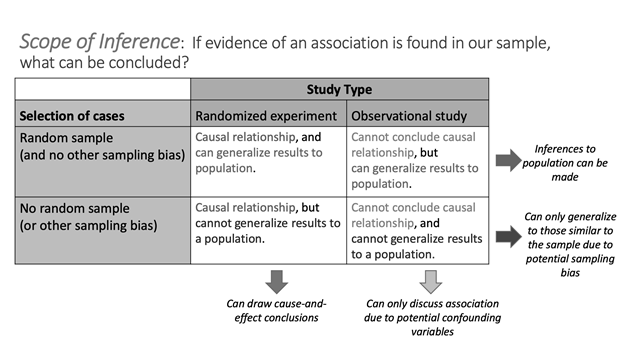
\includegraphics[width=0.75\linewidth]{images/ScopeOfInferenceGreyscale} \end{center}

\begin{enumerate}
\def\labelenumi{\arabic{enumi}.}
\setcounter{enumi}{17}
\item
  Use the table to determine the scope of inference for the study in question 1.
  \vspace{0.3in}
\item
  Use the table to determine the scope of inference for the study in question 2.
  \vspace{0.3in}
\end{enumerate}

\hypertarget{take-home-messages-3}{%
\subsection{Take-home messages}\label{take-home-messages-3}}

\begin{enumerate}
\def\labelenumi{\arabic{enumi}.}
\item
  The study design (observational study vs, experiment) determines if we can draw causal inferences or not. If an association is detected, a randomized experiment allows us to conclude that there is a causal (cause-and-effect) relationship between the explanatory and response variable. Observational studies have potential confounding variables within the study that prevent us from inferring a causal relationship between the variables studied.
\item
  Confounding variables are variables not included in the study that are related to both the explanatory and the response variables. When there are potential confounding variables in the study we cannot draw causal inferences.
\item
  Random assignment balances confounding variables across treatment groups. This eliminates any possible confounding variables by breaking the connections between the explanatory variable and the potential confounding variables.
\item
  Observational studies will always carry the possibility of confounding variables. Randomized experiments, which use random assignment, will have no confounding variables.
\end{enumerate}

\newpage

\hypertarget{additional-notes-3}{%
\subsection{Additional notes}\label{additional-notes-3}}

Use this space to summarize your thoughts and take additional notes on today's activity and material covered.

\newpage

\hypertarget{exploring-categorical-and-quantitative-data}{%
\chapter{Exploring Categorical and Quantitative Data}\label{exploring-categorical-and-quantitative-data}}

\hypertarget{week-3-reading-guide-introduction-to-r-categorical-variables-and-a-single-quantitative-variable}{%
\section{Week 3 Reading Guide: Introduction to R, Categorical Variables, and a Single Quantitative Variable}\label{week-3-reading-guide-introduction-to-r-categorical-variables-and-a-single-quantitative-variable}}

\hypertarget{chapter-3-applications-data}{%
\subsection*{Chapter 3 (Applications: Data)}\label{chapter-3-applications-data}}
\addcontentsline{toc}{subsection}{Chapter 3 (Applications: Data)}

\textbf{Videos}

\begin{itemize}
\tightlist
\item
  Starting\_with\_R
\end{itemize}

\setstretch{1.25}

\hypertarget{notes-3}{%
\subsubsection*{Notes}\label{notes-3}}
\addcontentsline{toc}{subsubsection}{Notes}

R is case sensitive, meaning it reads \texttt{data} differently from \texttt{Data}. If you get an error message, check that your capitalization is correct.

R does not like spaces or special characters. This means the column and row headers in the data set should not have spaces, periods, commas, etc. Instead of titling the variable \texttt{column\ header}, use \texttt{column\_header} or \texttt{ColumnHeader}.

\textbf{Tidy data}: Data frames should have

\rgi 1 row per \_\_\_\_\_\_\_\_\_\_\_\_\_\_\_\_,

\rgi 1 column per \_\_\_\_\_\_\_\_\_\_\_\_.

We highly recommend completing the R/RStudio tutorials in section 3 to help understand R better.

We will not expect you to be able to write full code independently for this course. For Stat 216, you will need to understand types (categorical or quantitative) and roles (explanatory or response) of variables, as well as the structure of data, in order to fill in a few blanks in provided code to graph or analyze data.

\hypertarget{functions}{%
\subsubsection*{Functions}\label{functions}}
\addcontentsline{toc}{subsubsection}{Functions}

State what these introductory functions do in R:

\texttt{glimpse(data\_set\_name)}

\texttt{head(data\_set\_name)}

\texttt{data\_set\_name\$variable\_name}

\texttt{\textless{}-}

\texttt{\%\textgreater{}\%}

\hypertarget{chapter-4-exploring-categorical-data}{%
\subsection*{Chapter 4 (Exploring categorical data)}\label{chapter-4-exploring-categorical-data}}
\addcontentsline{toc}{subsection}{Chapter 4 (Exploring categorical data)}

\setstretch{1}

\textbf{Videos}

\begin{itemize}
\tightlist
\item
  4.1
\item
  4.2
\item
  4.4
\end{itemize}

\setstretch{1.25}

\hypertarget{vocabulary-3}{%
\subsubsection*{Vocabulary}\label{vocabulary-3}}
\addcontentsline{toc}{subsubsection}{Vocabulary}

Frequency table:
\rgs

Relative frequency table:
\rgs

Contingency or two-way table:
\rgs

Association (between two variables):
\rgs

Unconditional proportion:
\rgs

Conditional proportion:
\rgs

\rgi Row proportions:
\rgs

\rgi Column proportions:
\rgs

Statistic:
\rgs

\rgi Sample proportion:
\rgs

\rgi \rgi Notation:
\rgs

Parameter:
\rgs

\rgi Population proportion:
\rgs

\rgi \rgi Notation:
\rgs

Bar plot:
\rgs

Segmented bar plot:
\rgs

Mosaic plot:
\rgs

Simpson's Paradox:
\rgs

\hypertarget{notes-4}{%
\subsubsection*{Notes}\label{notes-4}}
\addcontentsline{toc}{subsubsection}{Notes}

In a contingency table, which variable (explanatory or response) generally will make the columns of the table? Which variable will make the rows of the table?
\rgs

In a segmented bar plot, the bars represent the levels of which variable? The segments represent the levels of which variable?
\rgs

What type of plot(s) are appropriate to display a single categorical variable?
\rgs

What type of plot(s) are appropriate to display two categorical variables?
\rgs

What is the difference between a standardized segmented bar plot and a mosaic plot?
\rgs

True or false: Pie charts are generally highly recommended ways to graphically display categorical data.

True or false: Two categorical variables are associated if the conditional proportions of a particular outcome (typically of the response variable) differ across levels of the other variable (typically the explanatory variable).

True or false: When a segmented bar plot has segments that sum to 1 (or 100\%), the segment heights correspond to the proportions conditioned on the \textbf{segment}.

\hypertarget{review-of-simpsons-paradox}{%
\subsubsection*{Review of Simpson's Paradox}\label{review-of-simpsons-paradox}}
\addcontentsline{toc}{subsubsection}{Review of Simpson's Paradox}

Based on the segmented bar plot in Figure 4.6, which race of defendant was more likely to have the death penalty invoked?
\rgs

Based on the segmented bar plot in Figure 4.7 and Table 4.9, which race of defendant was more likely to have the death penalty invoked when the victim was Caucasian?
\rgs

Based on the segmented bar plot in Figure 4.7 and Table 4.9, which race of defendant was more likely to have the death penalty invoked when the victim was African American?
\rgs

The direction of the relationship between the \_\_\_\_\_\_\_\_\_\_\_\_\_\_
and \_\_\_\_\_\_\_\_\_\_\_\_\_\_ variables is \textbf{reversed} when accounting for
a \_\_\_\_\_\_\_\_\_\_\_\_\_\_ variable.
\rgs

\hypertarget{chapter-5-exploring-quantitative-data}{%
\subsection*{Chapter 5 (Exploring quantitative data)}\label{chapter-5-exploring-quantitative-data}}
\addcontentsline{toc}{subsection}{Chapter 5 (Exploring quantitative data)}

\textbf{Videos}

\begin{itemize}
\tightlist
\item
  5.2to5.4
\item
  5.5to5.6
\item
  5.7
\end{itemize}

\hypertarget{type-of-plots}{%
\subsubsection*{Type of Plots}\label{type-of-plots}}
\addcontentsline{toc}{subsubsection}{Type of Plots}

Scatterplot:
\rgs

Dot plot:
\rgs

Histogram:
\rgs

Density plot:
\rgs

Box plot:
\rgs

\hypertarget{vocabulary-4}{%
\subsubsection*{Vocabulary}\label{vocabulary-4}}
\addcontentsline{toc}{subsubsection}{Vocabulary}

Four characteristics of a scatterplot:

\rgi Form:
\rgs

\rgi Strength:
\rgs

\rgi Direction:
\rgs

\rgi Unusual observations or outliers:
\rgs

Distribution (of a variable):
\rgs

\rgi Four characteristics of the distribution of one quantitative variable:

\rgi Center:
\rgs

\rgi Variability:
\rgs

\rgi Shape:
\rgs

\rgi Outliers:
\rgs

Point estimate:
\rgs

Histogram:
\rgs

Data density:
\rgs

Tail:
\rgs

Skew:
\rgs

Symmetric:
\rgs

Modality:
\rgs

Density plot:
\rgs 

Deviation:
\rgs

Variance:
\rgs

Standard deviation:
\rgs

Boxplot:
\rgs

Five number summary:
\rgs

Median:
\rgs

\(X^{th}\) percentile:
\rgs

Interquartile range (IQR):
\rgs

Robust statistics:
\rgs

\hypertarget{notes-5}{%
\subsubsection*{Notes}\label{notes-5}}
\addcontentsline{toc}{subsubsection}{Notes}

What type of plot(s) are appropriate for displaying one quantitative variable?
\rgs

What type of plot(s) are appropriate for displaying two quantitative variables?
\rgs

What type of plot(s) are appropriate for displaying one quantitative variable and one categorical variable?
\rgs

What are the two ways to measure the `center' of a distribution? Which one is considered robust to skew/outliers?
\rgs

What are the three ways to measure the `variability' of a distribution? Which one is considered robust to skew/outliers?
\rgs

How are variance and standard deviation related?
\rgs

Fill in the following table with the appropriate notation.

\begin{center}
\begin{tabular}{|l|p{2in}|p{2in}|} \hline
Summary Measure & Parameter & Statistic \\ \hline
Mean & & \\ 
& & \\ \hline
Variance & & \\ 
& & \\ \hline
Standard deviation & & \\ 
& & \\ \hline
\end{tabular}
\end{center}

How are outliers denoted on a box plot? How can you mathematically determine if a data set has outliers?
\rgs

\hypertarget{summarizing-chapters-4-and-5}{%
\subsection{Summarizing Chapters 4 and 5}\label{summarizing-chapters-4-and-5}}

Look at the table of vocabulary terms in the final section of each chapter. If there are any you do not know, be sure to review the appropriate section of your text.

\hypertarget{notes-6}{%
\subsubsection*{Notes}\label{notes-6}}
\addcontentsline{toc}{subsubsection}{Notes}

Statistics summarize \_\_\_\_\_\_\_\_\_\_\_\_\_ .\\
Parameters summarize \_\_\_\_\_\_\_\_\_\_\_\_\_.

Fill in the following table with the appropriate notation for each summary measure.

\begin{center}
\begin{tabular}{|l|p{2in}|p{2in}|}\hline
Summary measure & Statistic & Parameter \\ \hline
Sample size & & \\ 
& & \\ 
& & \\ \hline
Proportion & & \\ 
(used to summarize & & \\ 
one categorical variable) & & \\ \hline
Mean & & \\ 
(used to summarize & & \\ 
one quantitative variable)& & \\ \hline
Correlation & & \\ 
(used to summarize & & \\ 
two quantitative variables)& & \\ \hline
Regression line slope & & \\ 
(used to summarize & & \\ 
two quantitative variables)& & \\ \hline
\end{tabular}
\end{center}

\hypertarget{data-visualization-summary}{%
\subsubsection*{Data visualization summary}\label{data-visualization-summary}}
\addcontentsline{toc}{subsubsection}{Data visualization summary}

Fill in the following table to help associate type of plot for each of several scenarios.

\begin{center}
\begin{tabular}{|l|p{3in}|} \hline
 & Appropriate plot(s) \\ \hline
One categorical variable & \\
(categorical response, no explanatory) & \\ \hline
One quantitative variable  & \\
(quantitative response, no explanatory) & \\ \hline
Two categorical variables  & \\
(categorical response, categorical explanatory) & \\ \hline
One of each  & \\
(quantitative response, categorical explanatory) & \\ \hline
Two quantitative variables  & \\
(quantitative response, quantitative explanatory) & \\ \hline
\end{tabular}
\end{center}

\rgs

\newpage

\hypertarget{activity-3-graphing-categorical-variables}{%
\section{Activity 3: Graphing Categorical Variables}\label{activity-3-graphing-categorical-variables}}

\setstretch{1}

\hypertarget{learning-outcomes-4}{%
\subsection{Learning outcomes}\label{learning-outcomes-4}}

\begin{itemize}
\item
  Identify and create appropriate summary statistics and plots given a data set or research question involving categorical variables.
\item
  Plots for a single categorical variable: bar plot.
\item
  Plots for association between two categorical variables:
  segmented bar plot, mosaic plot.
\end{itemize}

\hypertarget{terminology-review-4}{%
\subsection{Terminology review}\label{terminology-review-4}}

In today's activity, we will review summary measures and plots for categorical variables. Some terms covered in this activity are:

\begin{itemize}
\item
  Proportions
\item
  Bar plots
\item
  Segmented bar plots
\item
  Mosaic plots
\end{itemize}

To review these concepts, see Chapter 4 in the textbook.

\hypertarget{graphing-categorical-variables}{%
\subsection{Graphing categorical variables}\label{graphing-categorical-variables}}

For today's activity we will begin to use the statistical package R to analyze data through the IDE (integrated development environment) RStudio. For almost all activities and labs it will be necessary to upload the provided R script file from D2L for that day. Follow these steps to upload the necessary R script file for today's activity:

\begin{itemize}
\tightlist
\item
  Download the Myopia Activity R script file from D2L.
\item
  Click ``Upload'' in the ``Files'' tab in the bottom right window of RStudio. In the pop-up window, click ``Choose File'', and navigate to the folder where the Myopia Activity R script file is saved (most likely in your downloads folder). Click ``Open''; then click ``Ok''.
\item
  You should see the uploaded file appear in the list of files in the bottom right window.
\item
  Click on the file name to open the file in the Editor window (upper left window).
\end{itemize}

Notice that the first three lines of code contain a prompt called, \texttt{library}. Packages needed to run functions in R are stored in directories called libraries. When using the MSU RStudio server, all the packages needed for the class are already installed. We simply must tell R which packages we need for each R script file. We use the prompt \texttt{library} to load each \textbf{package} (or library) needed for each activity. Note, these \texttt{library} lines MUST be run each time you open a R script file in order for the functions in R to work. Before class today you should have worked through an R tutorial to prepare for class and to make sure you can login to the RStudio server. This tutorial will be a great resource as you begin to use R.

Highlight and run lines 1--3 to load the packages needed for today's activity. Notice the use of the \# symbol in the R script file. The \# sign is not part of the R code. It is used by these authors to add comments to the R code and explain what each call is telling the program to do.
R will ignore everything after a \# sign when executing the code. Refer to the instructions following the \# sign to understand what you need to enter in the code.

\hypertarget{nightlight-use-and-myopia}{%
\subsection*{Nightlight use and myopia}\label{nightlight-use-and-myopia}}
\addcontentsline{toc}{subsection}{Nightlight use and myopia}

In a study reported in Nature (Quinn et al. 1999), a survey of 479 children found that those who had slept with a nightlight or in a fully lit room before the age of 2 had a higher incidence of nearsightedness (myopia) later in childhood.

In this study, there are two variables studied: \texttt{Light}: level of light in room at night (no light, nightlight, full light) and \texttt{Sight}: level of myopia developed later in childhood (high myopia, myopia, no myopia).

\begin{enumerate}
\def\labelenumi{\arabic{enumi}.}
\tightlist
\item
  Which variable is the explanatory variable? Which is the response variable?
\end{enumerate}

\vspace{0.8in}

An important part of understanding data is to create visual pictures of what the data represent. In this activity, we will create graphical representations of categorical data.

\hypertarget{r-code}{%
\subsubsection*{R code}\label{r-code}}
\addcontentsline{toc}{subsubsection}{R code}

Throughout these activities, we will often include the R code you would use in order to produce output or plots. These ``code chunks'' appear in gray. In the code chunk below, we demonstrate how to read the data set into R using the \texttt{read.csv()} function. The line of code shown below (line 6 in the R script file) reads in the data set and names the data set (object) \texttt{myopia}. Highlight and run line 6 in the R script file to load the data from the Stat 216 webpage.

\begin{Shaded}
\begin{Highlighting}[]
\CommentTok{\# This will read in the data set}
\NormalTok{myopia }\OtherTok{\textless{}{-}} \FunctionTok{read.csv}\NormalTok{(}\StringTok{"https://math.montana.edu/courses/s216/data/ChildrenLightSight.csv"}\NormalTok{) }
\end{Highlighting}
\end{Shaded}

\begin{enumerate}
\def\labelenumi{\arabic{enumi}.}
\setcounter{enumi}{1}
\tightlist
\item
  Click on the data set name (\texttt{Myopia}) in the Environment tab (upper right window). This will open the data set in a 2nd tab in the Editor window (upper left window). R is case sensitive, which means that you must always type the name of a variable EXACTLY as it is written in the data set including upper and lower case letters and without misspellings! Write down the name of each variable (column names) as it is written in the data set.
\end{enumerate}

\vspace{0.3in}

\hypertarget{displaying-a-single-categorical-variable}{%
\subsubsection*{Displaying a single categorical variable}\label{displaying-a-single-categorical-variable}}
\addcontentsline{toc}{subsubsection}{Displaying a single categorical variable}

If we wanted to know how many children in our data set were in each level of myopia, we could create a frequency bar plot of the variable \texttt{Sight}. Enter the variable name, \texttt{Sight} (\emph{note the capital S}), for \texttt{variable} into the \texttt{ggplot} code at line 10 in the R script file. Highlight and run lines 9--15 to create the plot. Note: this is a \textbf{frequency} bar plot plotting counts (the number of children in each level of sight is displayed on the \(y\)-axis).

\begin{Shaded}
\begin{Highlighting}[]
\NormalTok{myopia }\SpecialCharTok{\%\textgreater{}\%} \CommentTok{\# Data set piped into...}
\FunctionTok{ggplot}\NormalTok{(}\FunctionTok{aes}\NormalTok{(}\AttributeTok{y =}\NormalTok{ variable)) }\SpecialCharTok{+}   \CommentTok{\# This specifies the variable}
  \FunctionTok{geom\_bar}\NormalTok{(}\AttributeTok{stat =} \StringTok{"count"}\NormalTok{) }\SpecialCharTok{+}  \CommentTok{\# Tell it to make a bar plot}
  \FunctionTok{labs}\NormalTok{(}\AttributeTok{title =} \StringTok{"Frequency Bar Plot of Level of Myopia"}\NormalTok{,  }\CommentTok{\# Give your plot a title}
       \AttributeTok{x =} \StringTok{"Frequency"}\NormalTok{,   }\CommentTok{\# Label the x axis}
       \AttributeTok{y =} \StringTok{"Level of Myopia"}\NormalTok{)  }\SpecialCharTok{+} \CommentTok{\# Label the y axis}
  \FunctionTok{coord\_flip}\NormalTok{()  }\CommentTok{\# Turn the bars so they are vertical}
\end{Highlighting}
\end{Shaded}

\begin{enumerate}
\def\labelenumi{\arabic{enumi}.}
\setcounter{enumi}{2}
\tightlist
\item
  Sketch the bar chart created below. Be sure to label the axes.
\end{enumerate}

\vspace{2in}

\begin{enumerate}
\def\labelenumi{\arabic{enumi}.}
\setcounter{enumi}{3}
\tightlist
\item
  Using the bar chart created, estimate how many children have some level of myopia.
\end{enumerate}

\vspace{0.2in}

We could also choose to display the data as a proportion in a \textbf{relative frequency} bar plot. To find the relative frequency, divide the count in each level of myopia by the sample size. These are sample proportions. Notice that in this code we told R to create a bar plot with proportions.

\begin{Shaded}
\begin{Highlighting}[]
\NormalTok{myopia }\SpecialCharTok{\%\textgreater{}\%} \CommentTok{\# Data set piped into...}
\FunctionTok{ggplot}\NormalTok{(}\FunctionTok{aes}\NormalTok{(}\AttributeTok{x =}\NormalTok{ Sight)) }\SpecialCharTok{+}   \CommentTok{\# This specifies the variable}
  \FunctionTok{geom\_bar}\NormalTok{(}\FunctionTok{aes}\NormalTok{(}\AttributeTok{y =}\NormalTok{ ..prop.., }\AttributeTok{group =} \DecValTok{1}\NormalTok{)) }\SpecialCharTok{+}  \CommentTok{\# Tell it to make a bar plot with proportions}
  \FunctionTok{labs}\NormalTok{(}\AttributeTok{title =} \StringTok{"Relative Frequency Bar Plot of Level of Myopia"}\NormalTok{,  }\CommentTok{\# Give your plot a title}
       \AttributeTok{x =} \StringTok{"Level of Myopia"}\NormalTok{,   }\CommentTok{\# Label the x axis}
       \AttributeTok{y =} \StringTok{"Relative Frequency"}\NormalTok{)  }\CommentTok{\# Label the y axis}
\end{Highlighting}
\end{Shaded}

\begin{center}\includegraphics[width=0.5\linewidth]{03-A04-EDA-categorical_files/figure-latex/unnamed-chunk-3-1} \end{center}

\begin{enumerate}
\def\labelenumi{\arabic{enumi}.}
\setcounter{enumi}{4}
\tightlist
\item
  Which features in the relative frequency bar plot are the same as the frequency bar plot? Which are different?
\end{enumerate}

\newpage

\hypertarget{displaying-two-categorical-variables}{%
\subsubsection*{Displaying two categorical variables}\label{displaying-two-categorical-variables}}
\addcontentsline{toc}{subsubsection}{Displaying two categorical variables}

Is there an association between the level of light in a room and the development of myopia? To examine the differences in level of myopia for the level of light, we would create a segmented bar plot of \texttt{Light} segmented by \texttt{Sight}. To create the segmented bar plot enter the variable name, \texttt{Light} for \texttt{explanatory} and the variable name, \texttt{Sight} for \texttt{response} in the R script file in line 27. Highlight and run lines 26--33.

\begin{Shaded}
\begin{Highlighting}[]
\NormalTok{myopia }\SpecialCharTok{\%\textgreater{}\%} \CommentTok{\# Data set piped into...}
\FunctionTok{ggplot}\NormalTok{(}\FunctionTok{aes}\NormalTok{(}\AttributeTok{x =}\NormalTok{ explanatory, }\AttributeTok{fill =}\NormalTok{ response)) }\SpecialCharTok{+}   \CommentTok{\# This specifies the variables}
  \FunctionTok{geom\_bar}\NormalTok{(}\AttributeTok{stat =} \StringTok{"count"}\NormalTok{, }\AttributeTok{position =} \StringTok{"fill"}\NormalTok{) }\SpecialCharTok{+}  \CommentTok{\# Tell it to make a stacked bar plot}
  \FunctionTok{labs}\NormalTok{(}\AttributeTok{title =} \StringTok{"Segmented Bar Plot of Night Light Use by Level of Myopia"}\NormalTok{,  }
       \CommentTok{\# Make sure to title your plot }
       \AttributeTok{x =} \StringTok{"Level of Light"}\NormalTok{,   }\CommentTok{\# Label the x axis}
       \AttributeTok{y =} \StringTok{""}\NormalTok{) }\SpecialCharTok{+}  \CommentTok{\# Remove y axis label}
    \FunctionTok{scale\_fill\_grey}\NormalTok{()  }\CommentTok{\# Make figure black and white}
\end{Highlighting}
\end{Shaded}

\begin{enumerate}
\def\labelenumi{\arabic{enumi}.}
\setcounter{enumi}{5}
\tightlist
\item
  Sketch the segmented bar plot created here. Be sure to label the axes.
\end{enumerate}

\vspace{2in}

\begin{enumerate}
\def\labelenumi{\arabic{enumi}.}
\setcounter{enumi}{6}
\tightlist
\item
  From the segmented bar plot, estimate the proportion of no myopia for those that used a nightlight.
\end{enumerate}

\vspace{0.5in}

\begin{enumerate}
\def\labelenumi{\arabic{enumi}.}
\setcounter{enumi}{7}
\tightlist
\item
  Which level of light has the highest proportion of \texttt{No\ Myopia}?
\end{enumerate}

\vspace{0.5in}

We could also plot the data using a mosaic plot. Fill in the variable name, \texttt{Light} for \texttt{explanatory} and the variable name, \texttt{Sight} for \texttt{response} in line 38 in the R script file. Highlight and run lines 36--43.

\begin{Shaded}
\begin{Highlighting}[]
\NormalTok{myopia }\SpecialCharTok{\%\textgreater{}\%} \CommentTok{\# Data set piped into...}
  \FunctionTok{ggplot}\NormalTok{() }\SpecialCharTok{+}   \CommentTok{\# This specifies the variables}
  \FunctionTok{geom\_mosaic}\NormalTok{(}\FunctionTok{aes}\NormalTok{(}\AttributeTok{x=}\FunctionTok{product}\NormalTok{(explanatory), }\AttributeTok{fill =}\NormalTok{ response)) }\SpecialCharTok{+}  \CommentTok{\# Tell it to make a mosaic plot}
  \FunctionTok{labs}\NormalTok{(}\AttributeTok{title =} \StringTok{"Mosaic Plot of Night Light Use by Level of Myopia"}\NormalTok{,  }
       \CommentTok{\# Make sure to title your plot }
       \AttributeTok{x =} \StringTok{"Level of Light"}\NormalTok{,   }\CommentTok{\# Label the x axis}
       \AttributeTok{y =} \StringTok{""}\NormalTok{) }\SpecialCharTok{+}  \CommentTok{\# Remove y axis label}
      \FunctionTok{scale\_fill\_grey}\NormalTok{()  }\CommentTok{\# Make figure black and white}
\end{Highlighting}
\end{Shaded}

\begin{enumerate}
\def\labelenumi{\arabic{enumi}.}
\setcounter{enumi}{8}
\tightlist
\item
  What is similar and what is different between the segmented bar chart and the mosaic bar chart?
\end{enumerate}

\vspace{1in}

\begin{enumerate}
\def\labelenumi{\arabic{enumi}.}
\setcounter{enumi}{9}
\tightlist
\item
  Explain why the bar for \texttt{Nightlight} is the widest in the mosaic plot.
\end{enumerate}

\vspace{0.8in}

Fill in the name of the explanatory variable and the response variable in line 46 in the R script file, highlight and run line 46 to get the counts for each combination of levels of variables.

\begin{Shaded}
\begin{Highlighting}[]
\NormalTok{myopia }\SpecialCharTok{\%\textgreater{}\%} \FunctionTok{group\_by}\NormalTok{(explanatory) }\SpecialCharTok{\%\textgreater{}\%} \FunctionTok{count}\NormalTok{(response)}
\end{Highlighting}
\end{Shaded}

\begin{enumerate}
\def\labelenumi{\arabic{enumi}.}
\setcounter{enumi}{10}
\tightlist
\item
  Fill in the following table with the values from the R output.
\end{enumerate}

\begin{center}
\begingroup
\setlength{\tabcolsep}{14pt} % Default value: 6pt
\renewcommand{\arraystretch}{2} % Default value: 1
\begin{tabular}{|c|c|c|c|c|}
\hline
 & \multicolumn{3}{|c|}{\textbf{Light Level}} & \\ \hline
\textbf{Myopia Level} & Full Light & Nightlight & No Light & Total \\ \hline
 High Myopia & & & & \\ \hline
 Myopia & & & & \\ \hline
 No Myopia & & & & \\ \hline
 Total & & & & \\ \hline  
\end{tabular}
\endgroup
\end{center}

\begin{enumerate}
\def\labelenumi{\arabic{enumi}.}
\setcounter{enumi}{11}
\tightlist
\item
  Calculate the proportion of children with high myopia. Use appropriate notation.
\end{enumerate}

\vspace{0.3in}

\begin{enumerate}
\def\labelenumi{\arabic{enumi}.}
\setcounter{enumi}{12}
\tightlist
\item
  Calculate the proportion of children with high myopia among those that slept with full light. Use appropriate notation.
\end{enumerate}

\vspace{0.3in}

\begin{enumerate}
\def\labelenumi{\arabic{enumi}.}
\setcounter{enumi}{13}
\tightlist
\item
  Calculate the proportion of children with high myopia among those that slept with no light. Use appropriate notation.
\end{enumerate}

\vspace{0.3in}

\begin{enumerate}
\def\labelenumi{\arabic{enumi}.}
\setcounter{enumi}{14}
\tightlist
\item
  Calculate the difference in proportion of children with high myopia for those that slept with full light minus those who slept with no light. Give the appropriate notation. Use full light minus no light as the order of subtraction.
\end{enumerate}

\vspace{0.3in}

\hypertarget{take-home-messages-4}{%
\subsection{Take-home messages}\label{take-home-messages-4}}

\begin{enumerate}
\def\labelenumi{\arabic{enumi}.}
\item
  Bar charts can be used to graphically display a single categorical variable either as counts or proportions. Segmented bar charts and mosaic plots are used to display two categorical variables.
\item
  Segmented bar charts always have a scale from 0 - 100\%. The bars represent the outcomes of the explanatory variable. Each bar is segmented by the response variable. If the heights of each segment are the same for each bar there is no association between variables.
\item
  Mosaic plots are similar to segmented bar charts but the widths of the bars also show the number of observations within each outcome.
\end{enumerate}

\hypertarget{additional-notes-4}{%
\subsection{Additional notes}\label{additional-notes-4}}

Use this space to summarize your thoughts and take additional notes on today's activity and material covered.

\newpage

\hypertarget{week-3-lab-ipeds}{%
\section{Week 3 Lab: IPEDs}\label{week-3-lab-ipeds}}

\setstretch{1}

\hypertarget{learning-outcomes-5}{%
\subsection{Learning outcomes}\label{learning-outcomes-5}}

\begin{itemize}
\item
  Identify and create appropriate summary statistics and plots
  given a data set or research question for quantitative data.
\item
  Interpret the following summary statistics in context:
  median, lower quartile, upper quartile,
  standard deviation, interquartile range.
\end{itemize}

\hypertarget{terminology-review-5}{%
\subsection{Terminology review}\label{terminology-review-5}}

In today's lab, we will review summary measures and plots for quantitative variables. Some terms covered in this activity are:

\begin{itemize}
\item
  Two measures of center: mean, median
\item
  Two measures of spread (variability): standard deviation, interquartile range (IQR)
\item
  Types of graphs: box plots, dot plots, histograms
\item
  Identify and create appropriate summary statistics and plots given a data set or research question for a single categorical and a single quantitative variable.
\item
  Interpret the following summary statistics in context:
  median, lower quartile, upper quartile,
  standard deviation, interquartile range.
\item
  Given a plot or set of plots, describe and compare the distribution(s)
  of a single quantitative variable
  (center, variability, shape, outliers).
\end{itemize}

To review these concepts, see Chapter 5 in the textbook.

\hypertarget{the-integrated-postsecondary-education-data-system-ipeds}{%
\subsection{The Integrated Postsecondary Education Data System (IPEDS)}\label{the-integrated-postsecondary-education-data-system-ipeds}}

Upload and open the provided R script file for the week 3 lab to answer the following questions. \textbf{Remember bolded questions will be answered on Gradescope for your group.}

These data are on a subset of institutions that met the following selection criteria (Education Statistics 2018):

\begin{itemize}
\item
  Degree granting
\item
  United States only
\item
  Title IV participating
\item
  Not for profit
\item
  2-year or 4-year or above
\item
  Has full-time first-time undergraduates
\item
  Note that several variables have missing values for some institutions (denoted by ``NA'').
\end{itemize}

\begin{center}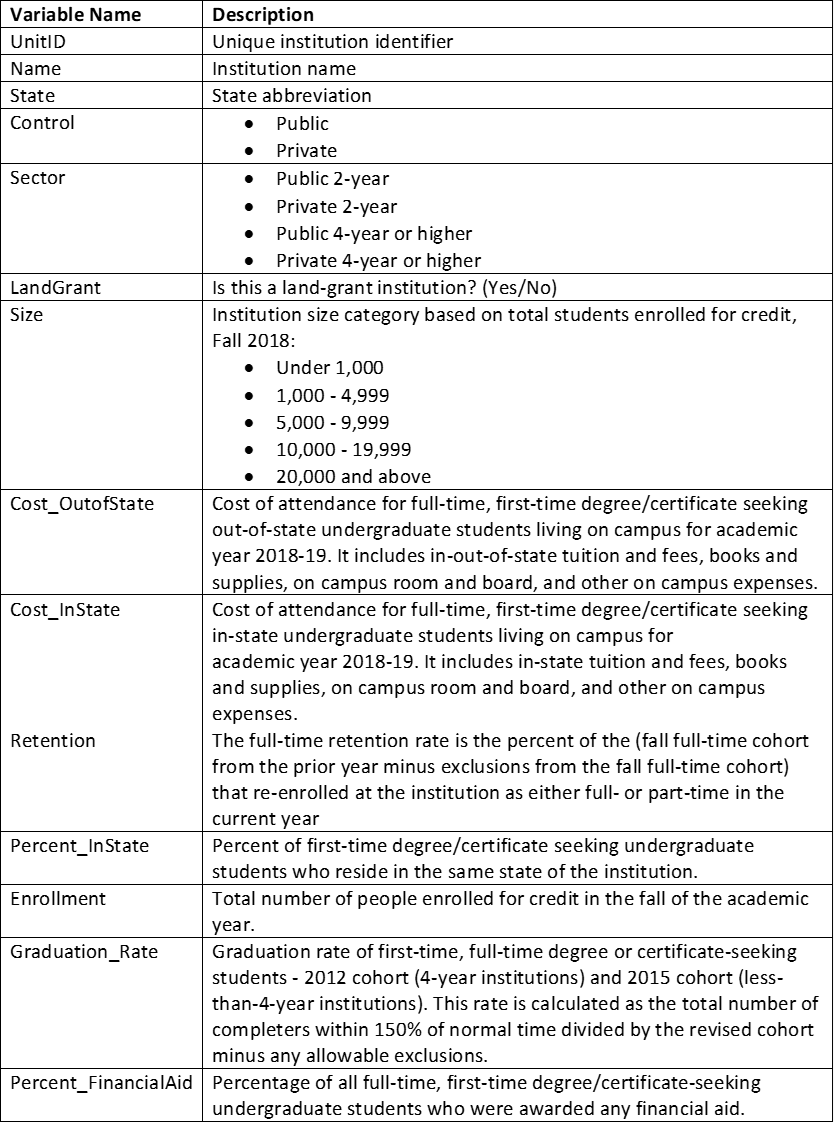
\includegraphics[width=0.75\linewidth]{images/IPEDS_Description} \end{center}

\hypertarget{summary-statistics-for-a-single-quantitative-variable}{%
\subsubsection*{Summary statistics for a single quantitative variable}\label{summary-statistics-for-a-single-quantitative-variable}}
\addcontentsline{toc}{subsubsection}{Summary statistics for a single quantitative variable}

Look through the provided chart above showing the description of variables measured. The UnitID and Name are identifiers for each observational unit, \emph{US degree granting institutions in 2018}.

\begin{enumerate}
\def\labelenumi{\arabic{enumi}.}
\tightlist
\item
  Identify in the chart above which variables collected on the US institutions are categorical (C) and which variables are quantitative (Q).
\end{enumerate}

\newpage

In Wednesday's activity, the code was provided to import the data set needed directly from the Stat 216 website. Follow these steps to upload and import the data set for today's lab.

\begin{itemize}
\item
  Download the provided data set \texttt{IPED\_Data\_2018} from D2L
\item
  Upload the data set \texttt{IPEDS\_Data\_2018} to the RStudio server using the same steps to upload the R script file.
\item
  Click on ``Import Dataset'' in the Environment tab in the upper right hand corner.
\item
  Choose ``From Text(base)'' in the drop-down menu and select the correct csv file.
\item
  Be sure that ``Yes'' is selected next to ``Heading'' in the pop-up screen. Click ``Import''.
\item
  To view the data set, click on the data set name (\texttt{IPEDS\_Data\_2018}). Verify that that column names match the first column in the chart on the previous page. If the columns are named V1, V2, V3\ldots etc, you did not select ``Yes'' for ``Heading''.
\end{itemize}

Enter the name of the data set (see the environment tab) for \texttt{datasetname} in the R script file in line 6. We will look at the retention rates for the 4-year institutions only. Enter the variable name \texttt{Retention} for \texttt{variable} in line 12. Highlight and run lines 1 -- 12. \textbf{Note that the two lines of code (lines 8 and 10) are filtering to remove the 2-year institutions so we are only assessing Public 4-year and Private 4-year institutions.} The \texttt{favstats()} function from the \texttt{mosaic} package gives the summary statistics for a quantitative variable. The summary statistics give the two measures of center and two measures of spread for retention rate.

\begin{Shaded}
\begin{Highlighting}[]
\NormalTok{IPEDS }\OtherTok{\textless{}{-}}\NormalTok{ datasetname }\CommentTok{\#Creates the object IPEDS }
\NormalTok{IPEDS }\OtherTok{\textless{}{-}}\NormalTok{ IPEDS }\SpecialCharTok{\%\textgreater{}\%}
  \FunctionTok{filter}\NormalTok{(Sector }\SpecialCharTok{!=} \StringTok{"Public 2{-}year"}\NormalTok{) }\CommentTok{\#Filters the data set to remove Public 2{-}year}
\NormalTok{IPEDS }\OtherTok{\textless{}{-}}\NormalTok{ IPEDS }\SpecialCharTok{\%\textgreater{}\%}
  \FunctionTok{filter}\NormalTok{(Sector }\SpecialCharTok{!=} \StringTok{"Private 2{-}year"}\NormalTok{) }\CommentTok{\#Filters the data set to remove Private 2{-}year}
\NormalTok{IPEDS }\SpecialCharTok{\%\textgreater{}\%}
  \FunctionTok{summarise}\NormalTok{(}\FunctionTok{favstats}\NormalTok{(variable)) }\CommentTok{\#Gives the summary statistics}
\end{Highlighting}
\end{Shaded}

\begin{enumerate}
\def\labelenumi{\arabic{enumi}.}
\setcounter{enumi}{1}
\tightlist
\item
  \textbf{Report the value for quartile 3 and interpret this value in context of the study.}
\end{enumerate}

\vspace{1in}

\begin{enumerate}
\def\labelenumi{\arabic{enumi}.}
\setcounter{enumi}{2}
\tightlist
\item
  Calculate the interquartile range (IQR = Q3 - Q1) for this study.
\end{enumerate}

\vspace{0.5in}

\begin{enumerate}
\def\labelenumi{\arabic{enumi}.}
\setcounter{enumi}{3}
\tightlist
\item
  Report and interpret the value of the standard deviation.
\end{enumerate}

\vspace{1in}

\begin{enumerate}
\def\labelenumi{\arabic{enumi}.}
\setcounter{enumi}{4}
\tightlist
\item
  How many missing values are there? What does this indicate?
\end{enumerate}

\vspace{0.8in}

\hypertarget{displaying-a-single-quantitative-variable}{%
\subsubsection*{Displaying a single quantitative variable}\label{displaying-a-single-quantitative-variable}}
\addcontentsline{toc}{subsubsection}{Displaying a single quantitative variable}

There are three type of plots used to plot a single quantitative variable: a dotplot, a histogram or a boxplot. A dotplot of retention rates would plot a dot for the retention rate for each 4-year institution.

We will create both a histogram and a boxplot of the variable \texttt{Retention}. Enter the name of the variable in both line 16 and line 23 for \texttt{variable} in the R script file. \textbf{Give each plot a descriptive title.} Highlight and run lines 15 -- 27 to give the histogram and boxplot. Notice that the \textbf{bin width} for the histogram is 10. For example, the first bin consists of the number of 4-year institutions in the data set with a retention rate of 0 to 10\%. It is important to note that a 4-year institution with a retention rate on the boundary of a bin will fall into the bin above it; for example, 10 would be counted in the bin 10--20.

\textbf{Export and upload both plots to Gradescope for your group.}

\begin{itemize}
\item
  To export the graphs: in the bottom right corner in the Plots tab, click on \texttt{Export}.
\item
  Then choose \texttt{Save\ as\ Image}. Save the image as a png. This will save your graph to the server.
\item
  In the Files tab, click on the box next to your saved image file, click \texttt{More} and choose \texttt{Export}. This will save your file to your downloads folder on your computer.
\end{itemize}

\begin{Shaded}
\begin{Highlighting}[]
\NormalTok{IPEDS }\SpecialCharTok{\%\textgreater{}\%} \CommentTok{\# Data set piped into...}
\FunctionTok{ggplot}\NormalTok{(}\FunctionTok{aes}\NormalTok{(}\AttributeTok{x =}\NormalTok{ variable)) }\SpecialCharTok{+}   \CommentTok{\# Name variable to plot}
  \FunctionTok{geom\_histogram}\NormalTok{(}\AttributeTok{binwidth =} \DecValTok{10}\NormalTok{) }\SpecialCharTok{+}  \CommentTok{\# Create histogram with specified binwidth }
  \FunctionTok{labs}\NormalTok{(}\AttributeTok{title =} \StringTok{"Title"}\NormalTok{, }\CommentTok{\# Title for plot}
       \AttributeTok{x =} \StringTok{"Rentention Rate"}\NormalTok{, }\CommentTok{\# Label for x axis}
       \AttributeTok{y =} \StringTok{"Frequency"}\NormalTok{) }\CommentTok{\# Label for y axis}
\end{Highlighting}
\end{Shaded}

\begin{Shaded}
\begin{Highlighting}[]
\NormalTok{IPEDS }\SpecialCharTok{\%\textgreater{}\%} \CommentTok{\# Data set piped into...}
\FunctionTok{ggplot}\NormalTok{(}\FunctionTok{aes}\NormalTok{(}\AttributeTok{x =}\NormalTok{ variable)) }\SpecialCharTok{+}   \CommentTok{\# Name variable to plot}
  \FunctionTok{geom\_boxplot}\NormalTok{() }\SpecialCharTok{+}  \CommentTok{\# Create boxplot }
  \FunctionTok{labs}\NormalTok{(}\AttributeTok{title =} \StringTok{"Title"}\NormalTok{, }\CommentTok{\# Title for plot}
       \AttributeTok{x =} \StringTok{"Retention Rates"}\NormalTok{, }\CommentTok{\# Label for x axis}
       \AttributeTok{y =} \StringTok{"Frequency"}\NormalTok{) }\CommentTok{\# Label for y axis}
\end{Highlighting}
\end{Shaded}

\begin{enumerate}
\def\labelenumi{\arabic{enumi}.}
\setcounter{enumi}{5}
\tightlist
\item
  What is the shape of the distribution of retention rates?
\end{enumerate}

\newpage

\begin{enumerate}
\def\labelenumi{\arabic{enumi}.}
\setcounter{enumi}{6}
\tightlist
\item
  Sketch the boxplot created and identify the values of the 5-number summary (minimum value, Q1, median, Q3, maximum value) on the plot. Use the following formulas to find the invisible fence on both ends of the distribution. Draw a dotted line at the invisible fence to show how the outliers were found.
\end{enumerate}

\[\text{Lower Fence: values} \le \text{Q}1 - 1.5\text{x}\text{IQR}\]

\[\text{Upper Fence: values} \ge \text{Q}3 + 1.5\text{x}\text{IQR}\]
\vspace{1.5in}

\hypertarget{robust-statistics}{%
\subsubsection*{Robust Statistics}\label{robust-statistics}}
\addcontentsline{toc}{subsubsection}{Robust Statistics}

Let's examine how the presence of outliers affect the values of center and spread.

\begin{enumerate}
\def\labelenumi{\arabic{enumi}.}
\setcounter{enumi}{7}
\tightlist
\item
  Report the two measures of center (mean and median) for retention given in the R output.
\end{enumerate}

\vspace{0.8in}

\begin{enumerate}
\def\labelenumi{\arabic{enumi}.}
\setcounter{enumi}{8}
\tightlist
\item
  Report the two measures of spread (standard deviation and IQR) for retention given in the R output.
\end{enumerate}

\vspace{0.8in}

\newpage

To show the effect of outliers on the measures of center and spread, the smallest values of retention rate in the data set were increased by 30\%. Highlight and run lines 30--38.

\begin{Shaded}
\begin{Highlighting}[]
\NormalTok{IPEDS }\SpecialCharTok{\%\textgreater{}\%} \CommentTok{\# Data set piped into...}
  \FunctionTok{summarise}\NormalTok{(}\FunctionTok{favstats}\NormalTok{(Retention\_Inc))}
\end{Highlighting}
\end{Shaded}

\begin{Shaded}
\begin{Highlighting}[]
\NormalTok{IPEDS }\SpecialCharTok{\%\textgreater{}\%} \CommentTok{\# Data set piped into...}
  \FunctionTok{ggplot}\NormalTok{(}\FunctionTok{aes}\NormalTok{(}\AttributeTok{x =}\NormalTok{ Retention\_Inc)) }\SpecialCharTok{+}   \CommentTok{\# Name variable to plot}
  \FunctionTok{geom\_boxplot}\NormalTok{() }\SpecialCharTok{+}  \CommentTok{\# Create boxplot}
  \FunctionTok{labs}\NormalTok{(}\AttributeTok{title =} \StringTok{"Boxplot of Adjusted Revenue of Movies in 2016"}\NormalTok{, }\CommentTok{\# Title for plot}
       \AttributeTok{x =} \StringTok{"Revenue (in Millions)"}\NormalTok{, }\CommentTok{\# Label for x axis}
       \AttributeTok{y =} \StringTok{"Frequency"}\NormalTok{) }\CommentTok{\# Label for y axis}
\end{Highlighting}
\end{Shaded}

\begin{enumerate}
\def\labelenumi{\arabic{enumi}.}
\setcounter{enumi}{9}
\tightlist
\item
  Report the two measures of center for this new data set.
\end{enumerate}

\vspace{0.8in}

\begin{enumerate}
\def\labelenumi{\arabic{enumi}.}
\setcounter{enumi}{10}
\tightlist
\item
  Report the two measures of spread for this new data set.
\end{enumerate}

\vspace{0.8in}

\begin{enumerate}
\def\labelenumi{\arabic{enumi}.}
\setcounter{enumi}{11}
\tightlist
\item
  \textbf{Which measure of center is robust to (not affected by) outliers? Explain your answer.}
\end{enumerate}

\vspace{0.5in}

\begin{enumerate}
\def\labelenumi{\arabic{enumi}.}
\setcounter{enumi}{12}
\tightlist
\item
  Which measure of spread is robust to outliers? Explain your answer.
\end{enumerate}

\vspace{0.5in}

\hypertarget{summarizing-a-single-categorical-and-single-quantitative-variable}{%
\subsubsection*{Summarizing a single categorical and single quantitative variable}\label{summarizing-a-single-categorical-and-single-quantitative-variable}}
\addcontentsline{toc}{subsubsection}{Summarizing a single categorical and single quantitative variable}

Is there a difference in retention rates for public and private 4-year institutions? In the next part of the activity we will compare retention rates for public and private 4-year institutions. Note that this variable (public or private) is labelled \texttt{Control} in the data set.

\begin{enumerate}
\def\labelenumi{\arabic{enumi}.}
\setcounter{enumi}{13}
\tightlist
\item
  \textbf{Based on the research question, which variable will we treat as the explanatory variable? Response variable?}
\end{enumerate}

\vspace{0.8in}

Enter the name of the explanatory variable and the name of the response variable in lines 42 and 45 of the R script file. Remember that the variable name must be typed in EXACTLY as it is written in the data set. Highlight and run lines 41 -- 49 to find the summary statistics and create side by side boxplots of the data.

\begin{Shaded}
\begin{Highlighting}[]
\NormalTok{IPEDS }\SpecialCharTok{\%\textgreater{}\%}  \CommentTok{\# Data set piped into...}
  \FunctionTok{summarise}\NormalTok{(}\FunctionTok{favstats}\NormalTok{(response}\SpecialCharTok{\textasciitilde{}}\NormalTok{explanatory)) }\CommentTok{\# Summary statistics for retention rates by sector}
\end{Highlighting}
\end{Shaded}

\begin{Shaded}
\begin{Highlighting}[]
\NormalTok{IPEDS }\SpecialCharTok{\%\textgreater{}\%}  \CommentTok{\# Data set piped into...}
  \FunctionTok{ggplot}\NormalTok{(}\FunctionTok{aes}\NormalTok{(}\AttributeTok{y =}\NormalTok{ response, }\AttributeTok{x =}\NormalTok{ explanatory))}\SpecialCharTok{+}  \CommentTok{\# Identify variables}
  \FunctionTok{geom\_boxplot}\NormalTok{()}\SpecialCharTok{+}  \CommentTok{\# Create box plot}
  \FunctionTok{labs}\NormalTok{(}\AttributeTok{title =} \StringTok{"Side by side box plot of retention rates by control"}\NormalTok{,  }\CommentTok{\# Title}
       \AttributeTok{x =} \StringTok{"Control"}\NormalTok{,    }\CommentTok{\# x{-}axis label}
       \AttributeTok{y =} \StringTok{"Retention Rates"}\NormalTok{)  }\CommentTok{\# y{-}axis label}
\end{Highlighting}
\end{Shaded}

\begin{enumerate}
\def\labelenumi{\arabic{enumi}.}
\setcounter{enumi}{14}
\item
  \textbf{Compare the two boxplots.}

  Which type of university has the highest center?
  \vspace{0.3in}

  Largest spread?
  \vspace{0.3in}

  What is the shape of each distribution?
  \vspace{0.3in}

  Does either distribution have outliers?
  \vspace{0.3in}
\item
  Report the difference in mean retention rates for private and public universities. Use private minus public as the order of subtraction. Use the appropriate notation.
\end{enumerate}

\vspace{0.8in}

\begin{enumerate}
\def\labelenumi{\arabic{enumi}.}
\setcounter{enumi}{16}
\tightlist
\item
  Does there appear to be an association between retention rates and type of university? Explain your answer.
\end{enumerate}

\newpage

\hypertarget{take-home-messages-5}{%
\subsection{Take-home messages}\label{take-home-messages-5}}

\begin{enumerate}
\def\labelenumi{\arabic{enumi}.}
\item
  Histograms, box plots, and dot plots can all be used to graphically display a single quantitative variable.
\item
  The box plot is created using the five number summary: minimum value, quartile 1, median, quartile 3, and maximum value. Values in the data set that are less than \(\text{Q}_1 - 1.5\text{xIQR}\) and greater than \(\text{Q}_3 + 1.5\text{xIQR}\) are considered outliers and are graphically represented by a dot outside of the whiskers on the box plot.
\item
  Data should be summarized numerically and displayed graphically to give us information about the study.
\item
  When comparing distributions of quantitative variables we look at the shape, center, spread, and for outliers. There are two measures of center: mean and the median and two measures of spread: standard deviation and the interquartile range, IQR = Q3 - Q1.
\item
  The median and the interquartile range are robust statistics, meaning that they are not affected by very large or very small values. When we have a skewed distribution the best measure of center is the median and the best measure of spread is the IQR.
\end{enumerate}

\newpage

\hypertarget{exploring-multivariable-data}{%
\chapter{Exploring Multivariable Data}\label{exploring-multivariable-data}}

\hypertarget{week-4-reading-guide-two-quantitative-variables-and-multivariable-concepts}{%
\section{Week 4 Reading Guide: Two Quantitative Variables and Multivariable Concepts}\label{week-4-reading-guide-two-quantitative-variables-and-multivariable-concepts}}

\hypertarget{section-6.1-fitting-a-line-residuals-and-correlation}{%
\subsection*{Section 6.1 (Fitting a line, residuals, and correlation)}\label{section-6.1-fitting-a-line-residuals-and-correlation}}
\addcontentsline{toc}{subsection}{Section 6.1 (Fitting a line, residuals, and correlation)}

\setstretch{1}

\textbf{Videos}

\begin{itemize}
\tightlist
\item
  6.1
\end{itemize}

\setstretch{1.25}

\hypertarget{reminders-from-section-5.1}{%
\subsubsection*{Reminders from Section 5.1}\label{reminders-from-section-5.1}}
\addcontentsline{toc}{subsubsection}{Reminders from Section 5.1}

Scatterplot: displays two quantitative variables; one dot = two measurements (\(x\), \(y\)) on one observational unit.

Four characteristics of a scatterplot:
\setstretch{1}

\begin{itemize}
\tightlist
\item
  \emph{Form}: pattern of the dots plotted. Is the trend generally linear (you can fit a straight line to the data) or non-linear?\\
\item
  \emph{Strength}: how closely do the points follow a trend? Very closely (strong)? No pattern (weak)?\\
\item
  \emph{Direction}: as the \(x\) values increase, do the \(y\)-values tend to increase (positive) or decrease (negative)?\\
\item
  Unusual observations or \emph{outliers}: points that do not fit the overall pattern of the data.
\end{itemize}

\setstretch{1.25}

\hypertarget{vocabulary-5}{%
\subsubsection*{Vocabulary}\label{vocabulary-5}}
\addcontentsline{toc}{subsubsection}{Vocabulary}

Predictor:
\rgs

Residual:
\rgs

\rgi Formula:
\rgs

Residual plot:
\rgs

Correlation:
\rgs

\hypertarget{notes-7}{%
\subsubsection*{Notes}\label{notes-7}}
\addcontentsline{toc}{subsubsection}{Notes}

General equation of a linear model for a \emph{population}: \(y= \beta_0+ \beta_1 x+\epsilon\), where

\rgi \(x\) represents
\rgs

\rgi \(y\) represents
\rgs

\rgi \(\beta_0\) represents
\rgs

\rgi \(\beta_1\) represents
\rgs

\rgi \(\epsilon\) represents
\rgs

General equation of a linear regression model from \emph{sample} data: \(\hat{y}= b_0+ b_1 x\), where

\rgi \(x\) represents
\rgs

\rgi \(\hat{y}\) represents
\rgs

\rgi \(b_0\) represents
\rgs

\rgi \(b_1\) represents
\rgs

Fill in the following table with the appropriate notation for each summary measure.

\begin{center}
\begin{tabular}{|l|p{2in}|p{2in}|} \hline
Summary Measure & Parameter & Statistic \\ \hline
Correlation & & \\ 
& & \\ \hline
Slope & & \\ 
& & \\ \hline
$y$-intercept & & \\ 
& & \\ \hline
\end{tabular}
\end{center}

Fill in the blanks below to define some of the properties of correlation:

\rgi The value of correlation must be between \_\_\_\_\_\_\_\_\_\_\_. (Includes the endpoints of the interval)

\rgi The sign of correlation gives the \_\_\_\_\_\_\_\_\_\_\_\_\_\_ of the linear relationship.

\rgi The magnitude of correlation gives the \_\_\_\_\_\_\_\_\_\_\_\_ of the linear relationship.

True or false: A scatterplot that shows random scatter would be considered non-linear.

True or false: If the correlation between two quantitative variables is equal to zero, then the two variables are not associated.

True or false: To calculate a predicted \(y\)-value from a given \(x\)-value, just look at the scatterplot and estimate the \(y\)-value.

True or false: A positive residual indicates the data point is above the regression line.

\hypertarget{example-brushtail-possums}{%
\subsubsection*{Example: Brushtail possums}\label{example-brushtail-possums}}
\addcontentsline{toc}{subsubsection}{Example: Brushtail possums}

\begin{enumerate}
\def\labelenumi{\arabic{enumi}.}
\item
  What are the observational units?\\
  \rgs
\item
  Look at the scatterplot in Figure 6.5.
\end{enumerate}

\rgi a) What is the explanatory variable? The response variable? What type is each?
\rgs

\rgi b) What is the form of the scatterplot?
\rgs

\rgi c) What is the direction of the scatterplot?
\rgs

\rgi d) What is the strength of the scatterplot?
\rgs

\rgi e) Are there any outliers on the scatterplot?
\rgs

\begin{enumerate}
\def\labelenumi{\arabic{enumi}.}
\setcounter{enumi}{2}
\item
  Write the equation of the regression line, in context (do not use \(x\) and \(y\), use variable names instead).
  \rgs
\item
  Calculate the predicted head length for a possum with a 76.0 cm total length.
  \rgs
\item
  One of the possums in the data set has a total length of 76.0 cm and a head length of 85.1 mm. Calculate the residual for this possum. Does this possum lie above or below the regression line?
  \rgs
\end{enumerate}

\hypertarget{section-6.2-least-squares-regression}{%
\subsection*{Section 6.2 (Least squares regression)}\label{section-6.2-least-squares-regression}}
\addcontentsline{toc}{subsection}{Section 6.2 (Least squares regression)}

\setstretch{1}

You may skip the special topic sections (6.2.7)

\textbf{Videos}

\begin{itemize}
\tightlist
\item
  6.2
\end{itemize}

\setstretch{1.25}

\hypertarget{vocabulary-6}{%
\subsubsection*{Vocabulary}\label{vocabulary-6}}
\addcontentsline{toc}{subsubsection}{Vocabulary}

Least squares criterion:
\rgs

Least squares line:
\rgs

\texttt{lm()} R function:
\rgi \texttt{name\_of\_model\ \textless{}-\ lm(response\ \textasciitilde{}\ explanatory,\ data\ =\ data\_set\_name)}

\rgs

slope:
\rgs

\(y\)-intercept:\\
\rgs

Extrapolation:
\rgs 

Coefficient of determination:

\rgi \(s_y^2\) (or SST) represents
\rgs

\rgi \(s_{RES}^2\) (or SSE) represents
\rgs

\hypertarget{notes-8}{%
\subsubsection*{Notes}\label{notes-8}}
\addcontentsline{toc}{subsubsection}{Notes}

Two methods for determining the best line:

\rgi 1.
\rgs

\rgi 2.
\rgs

Notation for the coefficient of determination:
\rgs

Formulas for calculating the coefficient of determination:
\rgs

True or false: A correlation between two quantitative variables implies a causal relationship exists between the variables.

True or false: The slope of the line tells us how much to expect the \(y\) variable to increase or decrease when the \(x\) variable increases by 1 unit.

True or false: The coefficient of determination is just the square of the correlation.

\hypertarget{example-elmhurst-college}{%
\subsubsection*{Example: Elmhurst College}\label{example-elmhurst-college}}
\addcontentsline{toc}{subsubsection}{Example: Elmhurst College}

\begin{enumerate}
\def\labelenumi{\arabic{enumi}.}
\item
  What are the observational units?\\
  \rgs
\item
  Look at the scatterplot in Figure 6.13.
\end{enumerate}

\rgi a) What is the explanatory variable? The response variable?\\
\rgs

\rgi b) What is the form of the scatterplot?\\
\rgs

\rgi c) What is the direction of the scatterplot?
\rgs

\rgi d) What is the strength of the scatterplot?
\rgs

\rgi e) Are there any outliers on the scatterplot?\\
\rgs

\begin{enumerate}
\def\labelenumi{\arabic{enumi}.}
\setcounter{enumi}{2}
\item
  Write the equation of the regression line, in context (do not use \(x\) and \(y\), use variable names instead).
  \rgs
\item
  Interpret the slope of the line, in the context of the problem. Remember that both family income and gift aid from the university are measured in \$1000s.
  \rgs
  \rgs
\item
  Interpret the \(y\)-intercept of the line, in the context of the problem. Remember that both family income and gift aid from the university are measured in \$1000s.
  \rgs
  \rgs
\item
  Is your interpretation in question 5 an example of extrapolation? Justify your answer.
  \rgs
\item
  Give and interpret, in context, the value of the coefficient of determination.
  \rgs
  \rgs
\end{enumerate}

\hypertarget{section-6.3-outliers-in-linear-regression}{%
\subsection*{Section 6.3 (Outliers in linear regression)}\label{section-6.3-outliers-in-linear-regression}}
\addcontentsline{toc}{subsection}{Section 6.3 (Outliers in linear regression)}

\setstretch{1}

\textbf{Videos}

\begin{itemize}
\tightlist
\item
  6.3
\end{itemize}

\setstretch{1.25}

\hypertarget{vocabulary-7}{%
\subsubsection*{Vocabulary}\label{vocabulary-7}}
\addcontentsline{toc}{subsubsection}{Vocabulary}

Outlier:
\rgs

Leverage:
\rgs

Influential point:
\rgs

\hypertarget{notes-9}{%
\subsubsection*{Notes}\label{notes-9}}
\addcontentsline{toc}{subsubsection}{Notes}

Investigate, but do not remove, outliers. Unless you find there was an actual error in the data collection, ignoring outliers can make models poor predictors!

True or false: All high leverage outliers are influential.

True or false: An outlier is considered high leverage if it is extreme in its \(x\)-value.

\hypertarget{section-6.4-chapter-6-review}{%
\subsection*{Section 6.4 (Chapter 6 review)}\label{section-6.4-chapter-6-review}}
\addcontentsline{toc}{subsection}{Section 6.4 (Chapter 6 review)}

\setstretch{1}

Look at the table of vocabulary terms in the final section of each chapter. If there are any you do not know, be sure to review the appropriate section of your text.

\hypertarget{notes-10}{%
\subsubsection*{Notes}\label{notes-10}}
\addcontentsline{toc}{subsubsection}{Notes}

Statistics summarize:
\rgs

Parameters summarize:
\rgs

Determine whether each of the following statements about the correlation coefficient are true or false:

\begin{enumerate}
\def\labelenumi{\arabic{enumi}.}
\item
  The correlation coefficient must be a positive number.
\item
  Stronger linear relationships are indicated by correlation coefficients far from 0.
\item
  The correlation coefficient is a robust statistic.
\item
  When two variables are highly correlated, that indicates a causal relationship exists between the variables.
\item
  The sign of the correlation coefficient will be the same as the sign of the regression line slope, though the values are typically different.
\end{enumerate}

Fill in the blanks to correctly interpret:

\begin{itemize}
\item
  Slope:

  For every \_\_\_\_\_\_\_\_\_\_\_\_\_\_\_\_\_\_\_\_\_\_\_\_\_\_\_\_, we expect \_\_\_\_\_\_\_\_\_\_\_\_\_\_\_\_\_ to increase (if slope is \_\_\_\_\_\_\_\_\_\_\_\_\_) or decrease (if slope is \_\_\_\_\_\_\_\_\_\_\_\_) by the absolute value of the \_\_\_\_\_\_\_\_\_.
\item
  \(y\)-intercept:

  If \_\_\_\_\_\_\_\_\_\_\_\_\_\_\_, we predict the \_\_\_\_\_\_\_\_\_\_\_\_\_\_\_\_\_\_\_\_\_\_\_\_\_\_ to equal \_\_\_\_\_\_\_\_\_\_.
\end{itemize}

Decision tree for determining an appropriate plot given a number of variables and their types from Chapter review:

\begin{center}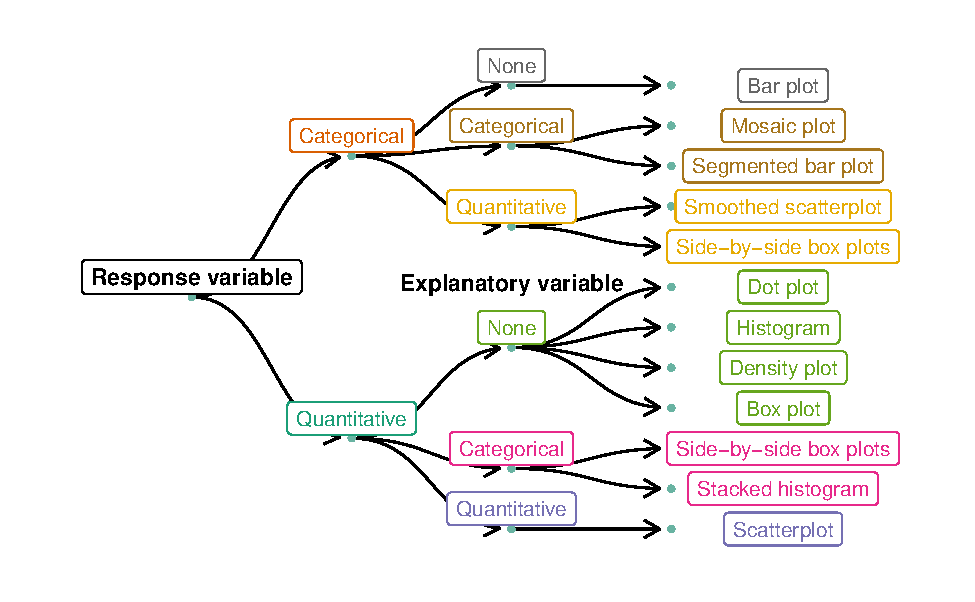
\includegraphics[width=0.7\linewidth]{04-RG-multivariate_files/figure-latex/decision-tree-plots-1} \end{center}

\hypertarget{section-7.1-gapminder-world}{%
\subsection*{Section 7.1 (Gapminder world)}\label{section-7.1-gapminder-world}}
\addcontentsline{toc}{subsection}{Section 7.1 (Gapminder world)}

\setstretch{1}

\textbf{Videos}

\begin{itemize}
\tightlist
\item
  Chapter7
\end{itemize}

\setstretch{1.25}

\hypertarget{vocabulary-8}{%
\subsubsection*{Vocabulary}\label{vocabulary-8}}
\addcontentsline{toc}{subsubsection}{Vocabulary}

Interaction:
\rgs

Aesthetic:
\rgs

\hypertarget{notes-11}{%
\subsubsection*{Notes}\label{notes-11}}
\addcontentsline{toc}{subsubsection}{Notes}

Use color and a legend to add a third variable to a scatterplot. E.g., Color the dots to represent different levels of a categorical variable or use shading of the dots to represent different values of a quantitative variable.

If the response and one predictor are quantitative and the other predictor is categorical, we fit a regression line for each level of the categorical predictor.

\begin{itemize}
\item
  Parallel slopes would indicate that that the two predictors \_\_\_\_\_\_\_\_\_\_\_\_\_\_\_\_\_\_\_ in explaining the response.
\item
  Non-parallel slopes would indicate that the two predictors \_\_\_\_\_\_\_\_\_\_\_\_\_\_\_\_\_\_\_ in explaining the response.
\end{itemize}

True or false: Scatterplots can only display two variables at a time.

\hypertarget{section-7.2-simpsons-paradox-revisited}{%
\subsection*{Section 7.2 (Simpson's Paradox, revisited)}\label{section-7.2-simpsons-paradox-revisited}}
\addcontentsline{toc}{subsection}{Section 7.2 (Simpson's Paradox, revisited)}

\setstretch{1}

\textbf{Videos}

\begin{itemize}
\tightlist
\item
  Chapter7
\end{itemize}

\setstretch{1.25}

\hypertarget{reminder-from-section-4.4}{%
\subsubsection*{Reminder from Section 4.4}\label{reminder-from-section-4.4}}
\addcontentsline{toc}{subsubsection}{Reminder from Section 4.4}

Simpson's Paradox: when the relationship between the explanatory and response variable is reversed when looking at the relationship within different levels of a confounding variable.

\hypertarget{notes-12}{%
\subsubsection*{Notes}\label{notes-12}}
\addcontentsline{toc}{subsubsection}{Notes}

True or false: Simpson's Paradox can only occur when the explanatory, response, and confounding variables are all categorical.

\hypertarget{example-sat-scores}{%
\subsubsection*{Example: SAT scores}\label{example-sat-scores}}
\addcontentsline{toc}{subsubsection}{Example: SAT scores}

\begin{enumerate}
\def\labelenumi{\arabic{enumi}.}
\item
  What are the observational units?\\
  \rgs
\item
  Look at the scatterplot in Figure 7.5.
\end{enumerate}

\rgi a) What is the explanatory variable? The response variable?
\rgs

\rgi b) What is the form of the scatterplot?
\rgs

\rgi c) What is the direction of the scatterplot?
\rgs

\rgi d) What is the strength of the scatterplot?
\rgs

\rgi e) Are there any outliers on the scatterplot?
\rgs

\begin{enumerate}
\def\labelenumi{\arabic{enumi}.}
\setcounter{enumi}{2}
\item
  What would need to be done to the study design in order to eliminate the confounding variable: percent of eligible students taking the SAT?
  \rgs
\item
  What features of the scatterplots in Figure 7.6 demonstrate that the percent of eligible students taking the SAT is a confounding variable?
  \rgs
\item
  How does Figure 7.7 demonstrate Simpson's Paradox?
  \rgs
\end{enumerate}

\newpage

\hypertarget{activity-4a-movie-profits-linear-regression}{%
\section{Activity 4A: Movie Profits --- Linear Regression}\label{activity-4a-movie-profits-linear-regression}}

\setstretch{1}

\hypertarget{learning-outcomes-6}{%
\subsection{Learning outcomes}\label{learning-outcomes-6}}

\begin{itemize}
\item
  Identify and create appropriate summary statistics and plots
  given a data set with two quantitative variables.
\item
  Use scatterplots to assess the relationship between two quantitative variables.
\item
  Find the estimated line of regression using summary statistics and R linear model (\texttt{lm()}) output.
\item
  Interpret the slope coefficient in context of the problem.
\end{itemize}

\hypertarget{terminology-review-6}{%
\subsection{Terminology review}\label{terminology-review-6}}

In today's activity, we will review summary measures and plots for two quantitative variables. Some terms covered in this activity are:

\begin{itemize}
\item
  Scatterplot
\item
  Least-squares line of regression
\item
  Slope and \(y\)-intercept
\item
  Residuals
\item
  Multivariable plots
\end{itemize}

To review these concepts, see Chapter 6 \& 7 in the textbook.

\hypertarget{movies-released-in-2016}{%
\subsection{Movies released in 2016}\label{movies-released-in-2016}}

A data set was collected on movies released in 2016 ({``{IMDb} Movies Extensive Dataset''} 2016). Here is a list of some of the variables collected on the observational units, movies released in 2016.

\begin{longtable}[]{@{}
  >{\raggedright\arraybackslash}p{(\columnwidth - 2\tabcolsep) * \real{0.2353}}
  >{\raggedright\arraybackslash}p{(\columnwidth - 2\tabcolsep) * \real{0.7647}}@{}}
\toprule()
\begin{minipage}[b]{\linewidth}\raggedright
\textbf{Variable}
\end{minipage} & \begin{minipage}[b]{\linewidth}\raggedright
\textbf{Description}
\end{minipage} \\
\midrule()
\endhead
\texttt{budget\_mil} & Amount of money (in US \$ millions) budgeted for the production of the movie \\
\texttt{revenue\_mil} & Amount of money (in US \$ millions) the movie made after release \\
\texttt{duration} & Length of the movie (in minutes) \\
\texttt{content\_rating} & Rating of the movie (\texttt{G}, \texttt{PG}, \texttt{PG-13}, R, \texttt{Not\ Rated}) \\
\texttt{imdb\_score} & IMDb user rating score from 1 to 10 \\
\texttt{genres} & Categories the movie falls into (e.g., Action, Drama, etc.) \\
\texttt{facebook\_likes} & Number of likes a movie receives on Facebook \\
\bottomrule()
\end{longtable}

\begin{Shaded}
\begin{Highlighting}[]
\NormalTok{movies }\OtherTok{\textless{}{-}} \FunctionTok{read.csv}\NormalTok{(}\StringTok{"https://math.montana.edu/courses/s216/data/Movies2016.csv"}\NormalTok{) }\CommentTok{\# Reads in data set }
\end{Highlighting}
\end{Shaded}

\hypertarget{vocabulary-review}{%
\subsubsection*{Vocabulary review}\label{vocabulary-review}}
\addcontentsline{toc}{subsubsection}{Vocabulary review}

To look at the relationship between two quantitative variables we will create a scatterplot with the explanatory variable on the x-axis and the response variable on the y-axis. We can also find three summary measures for the linear relationship between the two variables: regression slope, correlation and the coefficient of determination.

We will look at the relationship between budget and revenue for movies released in 2016. Upload and open the Movie Profits Activity 4A F22 Code R script file. Enter the explanatory variable name, \texttt{budget\_mil}, for \texttt{explanatory} and the response variable name, \texttt{revenue\_mil}, for \texttt{response} at line 7 in the R script file to create the scatterplot. (Note: both variables are measured in ``millions of dollars'' (\$MM).) Highlight and run lines 1--12.

\begin{Shaded}
\begin{Highlighting}[]
\NormalTok{movies }\SpecialCharTok{\%\textgreater{}\%} \CommentTok{\# Data set pipes into...}
\FunctionTok{ggplot}\NormalTok{(}\FunctionTok{aes}\NormalTok{(}\AttributeTok{x =}\NormalTok{ explanatory, }\AttributeTok{y =}\NormalTok{ response))}\SpecialCharTok{+}  \CommentTok{\# Specify variables}
  \FunctionTok{geom\_point}\NormalTok{() }\SpecialCharTok{+}  \CommentTok{\# Add scatterplot of points}
  \FunctionTok{labs}\NormalTok{(}\AttributeTok{x =} \StringTok{"Budget in Millions ($)"}\NormalTok{,  }\CommentTok{\# Label x{-}axis}
       \AttributeTok{y =} \StringTok{"Revenue in Millions ($)"}\NormalTok{,  }\CommentTok{\# Label y{-}axis}
       \AttributeTok{title =} \StringTok{"Revenue vs. Budget"}\NormalTok{) }\SpecialCharTok{+} \CommentTok{\# Be sure to title your plots}
  \FunctionTok{geom\_smooth}\NormalTok{(}\AttributeTok{method =} \StringTok{"lm"}\NormalTok{, }\AttributeTok{se =} \ConstantTok{FALSE}\NormalTok{)  }\CommentTok{\# Add regression line}
\end{Highlighting}
\end{Shaded}

\begin{enumerate}
\def\labelenumi{\arabic{enumi}.}
\tightlist
\item
  Sketch the scatterplot created from the code.
\end{enumerate}

\vspace{2in}

\begin{enumerate}
\def\labelenumi{\arabic{enumi}.}
\setcounter{enumi}{1}
\tightlist
\item
  Assess the four features of the scatterplot that describe this relationship. Describe each feature using a complete sentence!
\end{enumerate}

\begin{itemize}
\tightlist
\item
  Form (linear, non-linear)
\end{itemize}

\vspace{.2in}

\begin{itemize}
\tightlist
\item
  Direction (positive, negative)
\end{itemize}

\vspace{.2in}

\begin{itemize}
\tightlist
\item
  Strength
\end{itemize}

\vspace{.2in}

\begin{itemize}
\tightlist
\item
  Unusual observations or outliers
\end{itemize}

\vspace{.2in}

\begin{enumerate}
\def\labelenumi{\arabic{enumi}.}
\setcounter{enumi}{2}
\tightlist
\item
  Based on the plot, does there appear to be an association between budget and revenue? Explain.
\end{enumerate}

\vspace{1in}

\hypertarget{slope}{%
\subsubsection*{Slope}\label{slope}}
\addcontentsline{toc}{subsubsection}{Slope}

The linear model function in R (\texttt{lm()}) gives us the summary for the least squares regression line. The estimate for \texttt{(Intercept)} is the \(y\)-intercept for the line of least squares, and the estimate for \texttt{budget\_mil} (the \(x\)-variable name) is the value of \(b_1\), the slope. Run lines 16 -- 17 in the R script file to reproduce the linear model output found in the coursepack.

\begin{Shaded}
\begin{Highlighting}[]
\CommentTok{\# Fit linear model: y \textasciitilde{} x}
\NormalTok{revenueLM }\OtherTok{\textless{}{-}} \FunctionTok{lm}\NormalTok{(revenue\_mil }\SpecialCharTok{\textasciitilde{}}\NormalTok{ budget\_mil, }\AttributeTok{data=}\NormalTok{movies)}
\FunctionTok{summary}\NormalTok{(revenueLM)}\SpecialCharTok{$}\NormalTok{coefficients }\CommentTok{\# Display coefficient summary}
\end{Highlighting}
\end{Shaded}

\begin{verbatim}
#>              Estimate Std. Error  t value     Pr(>|t|)
#> (Intercept) 9.1693054  9.0175499 1.016829 3.119606e-01
#> budget_mil  0.9460001  0.1056786 8.951670 4.339561e-14
\end{verbatim}

\begin{enumerate}
\def\labelenumi{\arabic{enumi}.}
\setcounter{enumi}{3}
\tightlist
\item
  Write out the least squares regression line using the summary statistics provided above in context of the problem.
  \vspace{0.8in}
\end{enumerate}

You may remember from middle and high school that slope \(=\frac{\mbox{rise}}{\mbox{run}}\).

Using \(b_1\) to represent slope, we can write that as the fraction \(\frac{b_1}{1}\).

Therefore, the slope predicts how much the line will \emph{rise} for each \emph{run} of +1. In other words, as the \(x\) variable increases by 1 unit, the \(y\) variable is predicted to change (increase/decrease) by the value of slope.

\begin{enumerate}
\def\labelenumi{\arabic{enumi}.}
\setcounter{enumi}{4}
\tightlist
\item
  Interpret the value of slope in context of the problem.
\end{enumerate}

\vspace{.8in}

\begin{enumerate}
\def\labelenumi{\arabic{enumi}.}
\setcounter{enumi}{5}
\tightlist
\item
  Using the least squares line from question 4, predict the revenue for a movie with a budget of 165 \$MM.
\end{enumerate}

\vspace{.6in}

\begin{enumerate}
\def\labelenumi{\arabic{enumi}.}
\setcounter{enumi}{6}
\tightlist
\item
  Predict the revenue for a movie with a budget of 500 \$MM.
\end{enumerate}

\vspace{0.8in}

\begin{enumerate}
\def\labelenumi{\arabic{enumi}.}
\setcounter{enumi}{7}
\tightlist
\item
  The prediction in question 7 is an example of what?
\end{enumerate}

\vspace{0.3in}

\hypertarget{residuals}{%
\subsubsection*{Residuals}\label{residuals}}
\addcontentsline{toc}{subsubsection}{Residuals}

The model we are using assumes the relationship between the two variables follows a straight line. The residuals are the errors, or the variability in the response that hasn't been modeled by the line (model).

\begin{center}
Data = Model + Residual

$\implies$ Residual = Data $-$ Model

$e_i=y_i-\hat{y}_i$
\end{center}

\begin{enumerate}
\def\labelenumi{\arabic{enumi}.}
\setcounter{enumi}{8}
\tightlist
\item
  The movie \emph{Independence Day: Resurgence} had a budget of 165 \$MM and revenue of 102.315 \$MM. Find the residual for this movie.
\end{enumerate}

\vspace{.8in}

\begin{enumerate}
\def\labelenumi{\arabic{enumi}.}
\setcounter{enumi}{9}
\tightlist
\item
  Did the line of regression overestimate or underestimate the revenue for this movie?
\end{enumerate}

\vspace{.2in}

\hypertarget{multivariable-plots}{%
\subsubsection*{Multivariable plots}\label{multivariable-plots}}
\addcontentsline{toc}{subsubsection}{Multivariable plots}

What if we wanted to see if the relationship between movie budget and revenue differs if we add another variable into the picture? The following plot visualizes three variables, creating a \textbf{multivariable} plot.

\begin{Shaded}
\begin{Highlighting}[]
\NormalTok{movies }\SpecialCharTok{\%\textgreater{}\%} \CommentTok{\# Data set pipes into...}
  \FunctionTok{filter}\NormalTok{(content\_rating }\SpecialCharTok{!=} \StringTok{"Not Rated"}\NormalTok{) }\SpecialCharTok{\%\textgreater{}\%} \CommentTok{\# Remove Not Rated movies}
  \FunctionTok{ggplot}\NormalTok{(}\FunctionTok{aes}\NormalTok{(}\AttributeTok{x =}\NormalTok{ budget\_mil, }\AttributeTok{y =}\NormalTok{ revenue\_mil, }\AttributeTok{color =}\NormalTok{ content\_rating)) }\SpecialCharTok{+}  \CommentTok{\# Specify variables}
  \FunctionTok{geom\_point}\NormalTok{(}\FunctionTok{aes}\NormalTok{(}\AttributeTok{shape =}\NormalTok{ content\_rating), }\AttributeTok{size =} \DecValTok{3}\NormalTok{) }\SpecialCharTok{+}  \CommentTok{\# Add scatterplot of points}
  \FunctionTok{labs}\NormalTok{(}\AttributeTok{x =} \StringTok{"Budget in Millions ($)"}\NormalTok{,  }\CommentTok{\# Label x{-}axis}
       \AttributeTok{y =} \StringTok{"Revenue in Millions ($)"}\NormalTok{,  }\CommentTok{\# Label y{-}axis}
       \AttributeTok{color =} \StringTok{"content\_rating"}\NormalTok{,  }\CommentTok{\# Label legend}
       \AttributeTok{title =} \StringTok{"Revenue vs. Budget"}\NormalTok{) }\SpecialCharTok{+} \CommentTok{\# Be sure to tile your plots}
  \FunctionTok{geom\_smooth}\NormalTok{(}\AttributeTok{method =} \StringTok{"lm"}\NormalTok{, }\AttributeTok{se =} \ConstantTok{FALSE}\NormalTok{, }\AttributeTok{lwd =} \DecValTok{2}\NormalTok{) }\SpecialCharTok{+} \CommentTok{\# Add regression lines}
  \FunctionTok{scale\_color\_grey}\NormalTok{() }\CommentTok{\# Make black and white}
\end{Highlighting}
\end{Shaded}

\begin{center}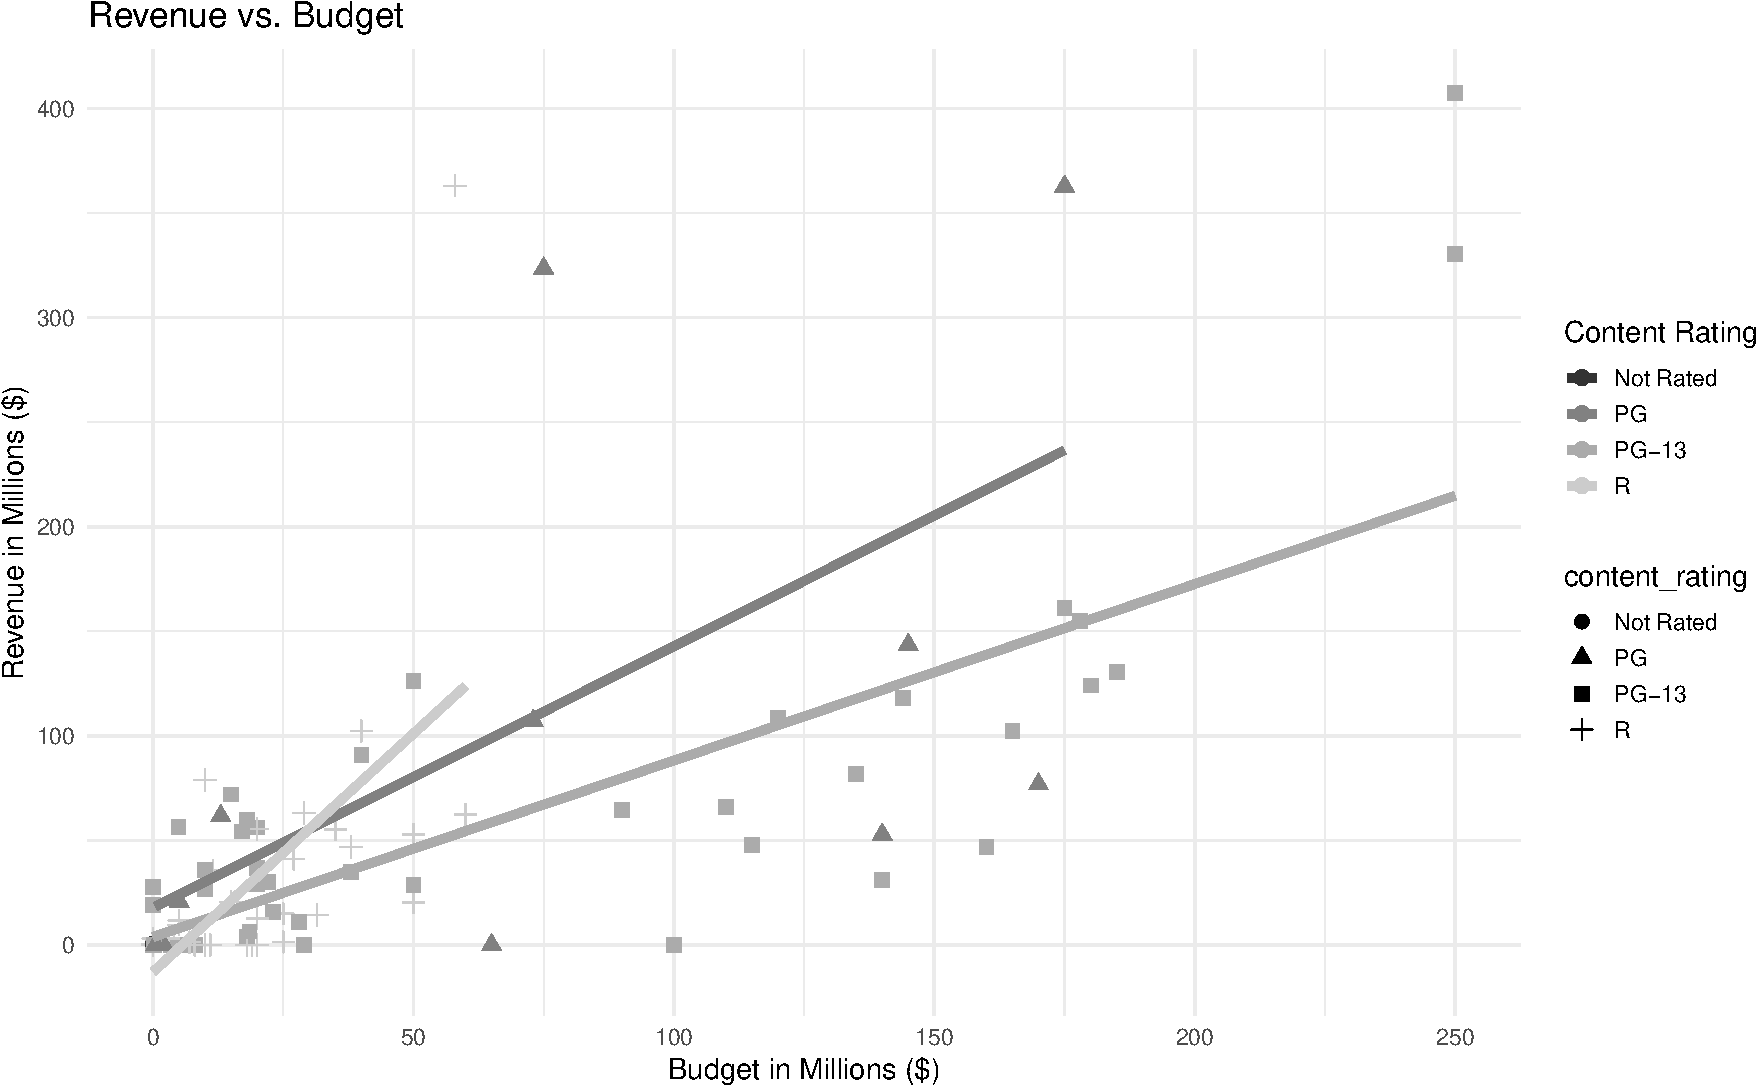
\includegraphics[width=0.7\linewidth]{04-A05-EDA-two-quantitative-PartA_files/figure-latex/unnamed-chunk-4-1} \end{center}

\begin{enumerate}
\def\labelenumi{\arabic{enumi}.}
\setcounter{enumi}{10}
\tightlist
\item
  Identify the three variables plotted in this graph.
\end{enumerate}

\vspace{0.5in}

\begin{enumerate}
\def\labelenumi{\arabic{enumi}.}
\setcounter{enumi}{11}
\tightlist
\item
  Does the \emph{relationship} between movie budget and revenue differ among the different content ratings? Explain.
\end{enumerate}

\vspace{0.8in}
\newpage

\hypertarget{take-home-messages-6}{%
\subsection{Take-home messages}\label{take-home-messages-6}}

\begin{enumerate}
\def\labelenumi{\arabic{enumi}.}
\item
  Two quantitative variables are graphically displayed in a scatterplot. The explanatory variable is on the \(x\)-axis and the response variable is on the \(y\)-axis. When describing the relationship between two quantitative variables we look at the form (linear or non-linear), direction (positive or negative), strength, and for the presence of outliers.
\item
  There are three summary statistics used to summarize the relationship between two quantitative variables: correlation (\(R\)), slope of the regression line (\(b_1\)), and the coefficient of determination (\(R^2\)).
\item
  We can use the line of regression to predict values of the response variable for values of the explanatory variable. Do not use values of the explanatory variable that are outside of the range of values in the data set to predict values of the response variable (reflect on why this is true.). This is called \textbf{extrapolation}.
\end{enumerate}

\hypertarget{additional-notes-5}{%
\subsection{Additional notes}\label{additional-notes-5}}

Use this space to summarize your thoughts and take additional notes on today's activity and material covered.

\newpage

\hypertarget{activity-4b-movie-profits-correlation-and-coefficient-of-determination}{%
\section{Activity 4B: Movie Profits --- Correlation and Coefficient of Determination}\label{activity-4b-movie-profits-correlation-and-coefficient-of-determination}}

\setstretch{1}

\hypertarget{learning-outcomes-7}{%
\subsection{Learning outcomes}\label{learning-outcomes-7}}

\begin{itemize}
\item
  Identify and create appropriate summary statistics and plots
  given a data set with two quantitative variables.
\item
  Calculate and interpret \(R^2\), the coefficient of determination, in context of the problem.
\item
  Find the correlation coefficient from R output or from \(R^2\) and the sign of the slope.
\end{itemize}

\hypertarget{terminology-review-7}{%
\subsection{Terminology review}\label{terminology-review-7}}

In today's activity, we will review summary measures and plots for two quantitative variables. Some terms covered in this activity are:

\begin{itemize}
\item
  Correlation (\(r\) or \(R\))
\item
  Coefficient of determination (\(r\)-squared or \(R^2\))
\end{itemize}

To review these concepts, see Chapter 6 in the textbook.

\hypertarget{movies-released-in-2016-1}{%
\subsection{Movies released in 2016}\label{movies-released-in-2016-1}}

We will revisit the movie data set collected on Movies released in 2016 ({``{IMDb} Movies Extensive Dataset''} 2016) to further explore the relationship between budget and revenue. Here is a reminder of the variables collected on these movies.

\begin{longtable}[]{@{}
  >{\raggedright\arraybackslash}p{(\columnwidth - 2\tabcolsep) * \real{0.2353}}
  >{\raggedright\arraybackslash}p{(\columnwidth - 2\tabcolsep) * \real{0.7647}}@{}}
\toprule()
\begin{minipage}[b]{\linewidth}\raggedright
\textbf{Variable}
\end{minipage} & \begin{minipage}[b]{\linewidth}\raggedright
\textbf{Description}
\end{minipage} \\
\midrule()
\endhead
\texttt{budget\_mil} & Amount of money (in US \$ millions) budgeted for the production of the movie \\
\texttt{revenue\_mil} & Amount of money (in US \$ millions) the movie made after release \\
\texttt{duration} & Length of the movie (in minutes) \\
\texttt{content\_rating} & Rating of the movie (\texttt{G}, \texttt{PG}, \texttt{PG-13}, R, \texttt{Not\ Rated}) \\
\texttt{imdb\_score} & IMDb user rating score from 1 to 10 \\
\texttt{genres} & Categories the movie falls into (e.g., Action, Drama, etc.) \\
\texttt{facebook\_likes} & Number of likes a movie receives on Facebook \\
\bottomrule()
\end{longtable}

\newpage

\hypertarget{correlation}{%
\subsubsection*{Correlation}\label{correlation}}
\addcontentsline{toc}{subsubsection}{Correlation}

Correlation measures the strength and the direction of the linear relationship between two quantitative variables. The closer the value of correlation to \(+1\) or \(-1\), the stronger the linear relationship. Values close to zero indicate a very weak linear relationship between the two variables. The following output shows a correlation matrix between several pairs of quantitative variables. Upload and open the Movie Profits Activity 4B F22 Code R script file. Highlight and run lines 1--12 to produce the same table as below.

\begin{Shaded}
\begin{Highlighting}[]
\NormalTok{movies }\OtherTok{\textless{}{-}} \FunctionTok{read.csv}\NormalTok{(}\StringTok{"https://math.montana.edu/courses/s216/data/Movies2016.csv"}\NormalTok{) }\CommentTok{\# Reads in data set}
\NormalTok{movies }\SpecialCharTok{\%\textgreater{}\%}  \CommentTok{\# Data set pipes into}
  \FunctionTok{select}\NormalTok{(}\FunctionTok{c}\NormalTok{(}\StringTok{"budget\_mil"}\NormalTok{, }\StringTok{"revenue\_mil"}\NormalTok{, }
           \StringTok{"duration"}\NormalTok{, }\StringTok{"imdb\_score"}\NormalTok{, }
           \StringTok{"facebook\_likes"}\NormalTok{)) }\SpecialCharTok{\%\textgreater{}\%}
  \FunctionTok{cor}\NormalTok{(}\AttributeTok{use=}\StringTok{"pairwise.complete.obs"}\NormalTok{) }\SpecialCharTok{\%\textgreater{}\%}
  \FunctionTok{round}\NormalTok{(}\DecValTok{3}\NormalTok{)}
\end{Highlighting}
\end{Shaded}

\begin{verbatim}
#>                budget_mil revenue_mil duration imdb_score facebook_likes
#> budget_mil          1.000       0.686    0.463      0.292          0.678
#> revenue_mil         0.686       1.000    0.227      0.398          0.723
#> duration            0.463       0.227    1.000      0.261          0.438
#> imdb_score          0.292       0.398    0.261      1.000          0.309
#> facebook_likes      0.678       0.723    0.438      0.309          1.000
\end{verbatim}

\begin{enumerate}
\def\labelenumi{\arabic{enumi}.}
\tightlist
\item
  Using the output above, which two variables have the \emph{strongest} correlation? What is the value of this correlation?
\end{enumerate}

\vspace{0.5in}

\begin{enumerate}
\def\labelenumi{\arabic{enumi}.}
\setcounter{enumi}{1}
\tightlist
\item
  What is the value of correlation between budget and revenue?
\end{enumerate}

\vspace{0.3in}

\begin{enumerate}
\def\labelenumi{\arabic{enumi}.}
\setcounter{enumi}{2}
\tightlist
\item
  Based on the value of correlation found in question 2, what would the sign of the slope be? Positive or negative? Explain.
\end{enumerate}

\vspace{0.5in}

\begin{enumerate}
\def\labelenumi{\arabic{enumi}.}
\setcounter{enumi}{3}
\tightlist
\item
  Does your answer to question 3 match the direction you choose in question 2 in Activity 4A?
\end{enumerate}

\vspace{0.3in}

\begin{enumerate}
\def\labelenumi{\arabic{enumi}.}
\setcounter{enumi}{4}
\tightlist
\item
  Explain why the correlation values on the diagonal are equal to 1.
\end{enumerate}

\vspace{0.8in}
\newpage

\hypertarget{coefficient-of-determination-squared-correlation}{%
\subsubsection*{Coefficient of determination (squared correlation)}\label{coefficient-of-determination-squared-correlation}}
\addcontentsline{toc}{subsubsection}{Coefficient of determination (squared correlation)}

Another summary measure used to explain the linear relationship between two quantitative variables is the coefficient of determination (\(r^2\)). The coefficient of determination, \(r^2\), can also be used to describe the strength of the linear relationship between two quantitative variables. The value of \(r^2\) (a value between 0 and 1) represents the \textbf{proportion of variation in the response that is explained by the least squares line with the explanatory variable}. There are two ways to calculate the coefficient of determination:

~~~Square the correlation coefficient: \(R^2 = (R)^2\)

~~~Use the variances of the response and the residuals: \(R^2 = \dfrac{s_y^2 - s_{RES}^2}{s_y^2} = \dfrac{SST - SSE}{SST}\)

\begin{enumerate}
\def\labelenumi{\arabic{enumi}.}
\setcounter{enumi}{5}
\tightlist
\item
  Use the correlation, \(R\), found in question 2 of the activity, to calculate the coefficient of determination between budget and revenue, \(R^2\).
\end{enumerate}

\vspace{.4in}

\begin{enumerate}
\def\labelenumi{\arabic{enumi}.}
\setcounter{enumi}{6}
\tightlist
\item
  The variance of the response variable, revenue in \$MM, is about \(s_{revenue}^2 = 8024.261\) \$MM\(^2\) and the variability in the residuals is about \(s_{RES}^2 = 4244.832\) \$MM\(^2\). Use these values to calculate the coefficient of determination. Verify that your answers to 6 and 7 are the same.
\end{enumerate}

\vspace{1in}

In the next part of the activity we will explore what the coefficient of determination measures.

\begin{itemize}
\item
  Go to the website www.rossmanchance.com/ISIapplets.html and click on Corr/Regresssion under Quantitative Response.
\item
  Click \texttt{Clear} below the box containing the sample data.
\item
  Download and open the csv file ``Movie2016'' from D2L. Copy the two columns containing \texttt{budget\_mil} and \texttt{revenue\_mil} including the headers and paste into the sample data box.
\item
  Click 'Use Data`.
\end{itemize}

\begin{enumerate}
\def\labelenumi{\arabic{enumi}.}
\setcounter{enumi}{7}
\tightlist
\item
  Click on \texttt{Show\ Moveable\ Line}. Write down the equation of the line given. Why is the slope zero for this line?
\end{enumerate}

\vspace{0.8in}

\begin{enumerate}
\def\labelenumi{\arabic{enumi}.}
\setcounter{enumi}{8}
\tightlist
\item
  Click on \texttt{Show\ Squared\ Residuals}. Write down the value for SSE. Since this is the sum of squared errors (SSE) for the horizontal line we call this the total sum of squares (SST).
\end{enumerate}

\newpage

\begin{enumerate}
\def\labelenumi{\arabic{enumi}.}
\setcounter{enumi}{9}
\tightlist
\item
  Click on \texttt{Show\ Regression\ Line}. Write down the equation of the line given. Does this match the least squares line found in Activity 4A question 4?
\end{enumerate}

\vspace{1in}

\begin{enumerate}
\def\labelenumi{\arabic{enumi}.}
\setcounter{enumi}{10}
\tightlist
\item
  Click on \texttt{Show\ Squared\ Residuals}. Write down the value for SSE.
\end{enumerate}

\vspace{0.5in}

\begin{enumerate}
\def\labelenumi{\arabic{enumi}.}
\setcounter{enumi}{11}
\tightlist
\item
  Calculate the value for \(R^2\) using the values found for SST and SSE.
\end{enumerate}

\vspace{1in}

\begin{enumerate}
\def\labelenumi{\arabic{enumi}.}
\setcounter{enumi}{12}
\tightlist
\item
  Write a sentence interpreting the coefficient of determination in context of the problem.
\end{enumerate}

\newpage

\hypertarget{take-home-messages-7}{%
\subsection{Take-home messages}\label{take-home-messages-7}}

\begin{enumerate}
\def\labelenumi{\arabic{enumi}.}
\item
  The sign of correlation and the sign of the slope will always be the same. The closer the value of correlation is to \(-1\) or \(+1\), the stronger the relationship between the explanatory and the response variable.
\item
  The coefficient of determination multiplied by 100 (\(R^2 \times 100\)) measures the percent of variation in the response variable that is explained by the relationship with the explanatory variable. The closer the value of the coefficient of determination is to 100\%, the stronger the relationship.
\end{enumerate}

\hypertarget{additional-notes-6}{%
\subsection{Additional notes}\label{additional-notes-6}}

Use this space to summarize your thoughts and take additional notes on today's activity and material covered.

\newpage

\hypertarget{week-4-lab-penguins}{%
\section{Week 4 Lab: Penguins}\label{week-4-lab-penguins}}

\setstretch{1}

\hypertarget{learning-outcomes-8}{%
\subsection{Learning outcomes}\label{learning-outcomes-8}}

\begin{itemize}
\item
  Identify and create appropriate summary statistics and plots
  given a data set with two quantitative variables.
\item
  Use scatterplots to assess the relationship between two quantitative variables.
\item
  Find the estimated line of regression using summary statistics and R linear model (\texttt{lm()}) output.
\item
  Interpret the slope coefficient in context of the problem.
\item
  Calculate and interpret \(R^2\), the coefficient of determination, in context of the problem.
\item
  Find the correlation coefficient from R output or from \(R^2\) and the sign of the slope.
\end{itemize}

\hypertarget{penguins}{%
\subsection{Penguins}\label{penguins}}

The Palmer Station Long Term Ecological Research Program sampled three penguin species on islands in the Palmer Archipelago in Antarctica. Researchers took various body measurements on the penguins, including flipper length and body mass. The researchers were interested in the relationship between flipper length and body mass and wondered if flipper length could be used to accurately predict the body mass of these three penguin species.

Upload and import the \texttt{Antarctica\_Penguins} csv file and the provided R script file for week 4 lab. Enter the name of the data set (see the environment tab) for \texttt{datasetname} in the R script file in line 4.

First we will create a scatterplot of the flipper length and body mass. Notice that we are using flipper length to predict body mass. This makes flipper length the explanatory variable. \textbf{Make sure to give your plot a descriptive title.} Highlight and run lines 1--13 in the R script file. \textbf{Upload a copy of your scatterplot to Gradescope.}

\begin{Shaded}
\begin{Highlighting}[]
\NormalTok{penguins }\OtherTok{\textless{}{-}}\NormalTok{ datasetname }\CommentTok{\#Creates the object penguins}
\NormalTok{penguins }\SpecialCharTok{\%\textgreater{}\%}
  \FunctionTok{ggplot}\NormalTok{(}\FunctionTok{aes}\NormalTok{(}\AttributeTok{x =}\NormalTok{ flipper\_length\_mm, }\AttributeTok{y =}\NormalTok{ body\_mass\_g))}\SpecialCharTok{+}  \CommentTok{\# Specify variables}
  \FunctionTok{geom\_point}\NormalTok{() }\SpecialCharTok{+}  \CommentTok{\# Add scatterplot of points}
  \FunctionTok{labs}\NormalTok{(}\AttributeTok{x =} \StringTok{"flipper length (mm)"}\NormalTok{,  }\CommentTok{\# Label x{-}axis}
       \AttributeTok{y =} \StringTok{"body mass (g)"}\NormalTok{,  }\CommentTok{\# Label y{-}axis}
       \AttributeTok{title =} \StringTok{"Title"}\NormalTok{) }\SpecialCharTok{+} \CommentTok{\# Be sure to title your plots}
  \FunctionTok{geom\_smooth}\NormalTok{(}\AttributeTok{method =} \StringTok{"lm"}\NormalTok{, }\AttributeTok{se =} \ConstantTok{FALSE}\NormalTok{)  }\CommentTok{\# Add regression line}
\end{Highlighting}
\end{Shaded}

\begin{enumerate}
\def\labelenumi{\arabic{enumi}.}
\tightlist
\item
  Assess the four features of the scatterplot that describe this relationship.
  \vspace{1mm}
\end{enumerate}

\begin{itemize}
\tightlist
\item
  Form (linear, non-linear)
\end{itemize}

\vspace{.1in}

\begin{itemize}
\tightlist
\item
  Direction (positive, negative)
\end{itemize}

\vspace{.1in}

\begin{itemize}
\tightlist
\item
  Strength
\end{itemize}

\vspace{.1in}

\begin{itemize}
\tightlist
\item
  Unusual observations or outliers
\end{itemize}

\vspace{.1in}

Highlight and run lines 16--20 to get the correlation matrix in the R script file.

\begin{Shaded}
\begin{Highlighting}[]
\NormalTok{penguins }\SpecialCharTok{\%\textgreater{}\%}  \CommentTok{\# Data set pipes into}
  \FunctionTok{select}\NormalTok{(}\FunctionTok{c}\NormalTok{(}\StringTok{"bill\_length\_mm"}\NormalTok{, }\StringTok{"bill\_depth\_mm"}\NormalTok{, }
           \StringTok{"flipper\_length\_mm"}\NormalTok{, }\StringTok{"body\_mass\_g"}\NormalTok{)) }\SpecialCharTok{\%\textgreater{}\%}
  \FunctionTok{cor}\NormalTok{(}\AttributeTok{use=}\StringTok{"pairwise.complete.obs"}\NormalTok{) }\SpecialCharTok{\%\textgreater{}\%}
  \FunctionTok{round}\NormalTok{(}\DecValTok{3}\NormalTok{)}
\end{Highlighting}
\end{Shaded}

\begin{enumerate}
\def\labelenumi{\arabic{enumi}.}
\setcounter{enumi}{1}
\tightlist
\item
  Using the R output, which two variables have the \emph{strongest} correlation? What is the value of this correlation?
\end{enumerate}

\vspace{0.5in}

\begin{enumerate}
\def\labelenumi{\arabic{enumi}.}
\setcounter{enumi}{2}
\tightlist
\item
  Using the value of correlation found in question 2, calculate the value of the coefficient of determination.
\end{enumerate}

\vspace{0.5in}

\begin{enumerate}
\def\labelenumi{\arabic{enumi}.}
\setcounter{enumi}{3}
\tightlist
\item
  \textbf{Interpret the coefficient of determination in context of the problem.}
\end{enumerate}

\vspace{1in}

Enter the variable \texttt{body\_mass\_g} for \texttt{response} and the variable name \texttt{flipper\_length\_mm} for \texttt{explanatory} in line 23 in the R script file. Highlight and run lines 23--24 to get the linear model output.

\begin{Shaded}
\begin{Highlighting}[]
\CommentTok{\# Fit linear model: y \textasciitilde{} x}
\NormalTok{penguinsLM }\OtherTok{\textless{}{-}} \FunctionTok{lm}\NormalTok{(response}\SpecialCharTok{\textasciitilde{}}\NormalTok{explanatory, }\AttributeTok{data=}\NormalTok{penguins)}
\FunctionTok{summary}\NormalTok{(penguinsLM)}\SpecialCharTok{$}\NormalTok{coefficients }\CommentTok{\# Display coefficient summary}
\end{Highlighting}
\end{Shaded}

\begin{enumerate}
\def\labelenumi{\arabic{enumi}.}
\setcounter{enumi}{4}
\tightlist
\item
  Write out the least squares regression line using the summary statistics from the R output in context of the problem.
\end{enumerate}

\vspace{.5in}

\begin{enumerate}
\def\labelenumi{\arabic{enumi}.}
\setcounter{enumi}{5}
\tightlist
\item
  \textbf{Interpret the value of slope in context of the problem.}
\end{enumerate}

\vspace{.8in}

\begin{enumerate}
\def\labelenumi{\arabic{enumi}.}
\setcounter{enumi}{6}
\tightlist
\item
  \textbf{Using the least squares regression line from question 5, predict the body mass for a penguin with a flipper length of 181 mm.}
\end{enumerate}

\vspace{.6in}

\begin{enumerate}
\def\labelenumi{\arabic{enumi}.}
\setcounter{enumi}{7}
\tightlist
\item
  One penguin had a flipper length of 181 mm and a body mass of 3750 g. Find the residual for this penguin.
\end{enumerate}

\vspace{.8in}

\begin{enumerate}
\def\labelenumi{\arabic{enumi}.}
\setcounter{enumi}{8}
\tightlist
\item
  Did the line of regression overestimate or underestimate the body mass for this penguin?
\end{enumerate}

\vspace{0.5in}

Highlight and run lines 27--34 to get the multivariate plot.

\begin{Shaded}
\begin{Highlighting}[]
\NormalTok{penguins }\SpecialCharTok{\%\textgreater{}\%}
  \FunctionTok{ggplot}\NormalTok{(}\FunctionTok{aes}\NormalTok{(}\AttributeTok{x =}\NormalTok{ flipper\_length\_mm, }\AttributeTok{y =}\NormalTok{ body\_mass\_g, }\AttributeTok{color=}\NormalTok{species))}\SpecialCharTok{+}  \CommentTok{\# Specify variables}
  \FunctionTok{geom\_point}\NormalTok{(}\FunctionTok{aes}\NormalTok{(}\AttributeTok{shape =}\NormalTok{ species), }\AttributeTok{size =} \DecValTok{3}\NormalTok{) }\SpecialCharTok{+}  \CommentTok{\# Add scatterplot of points}
  \FunctionTok{labs}\NormalTok{(}\AttributeTok{x =} \StringTok{"flipper length (mm)"}\NormalTok{,  }\CommentTok{\# Label x{-}axis}
       \AttributeTok{y =} \StringTok{"body mass (g)"}\NormalTok{,  }\CommentTok{\# Label y{-}axis}
       \AttributeTok{color =} \StringTok{"species"}\NormalTok{,}
       \AttributeTok{title =} \StringTok{"TITLE"}\NormalTok{) }\SpecialCharTok{+} \CommentTok{\# Be sure to tile your plots}
  \FunctionTok{geom\_smooth}\NormalTok{(}\AttributeTok{method =} \StringTok{"lm"}\NormalTok{, }\AttributeTok{se =} \ConstantTok{FALSE}\NormalTok{)  }\CommentTok{\# Add regression line}
\end{Highlighting}
\end{Shaded}

\begin{enumerate}
\def\labelenumi{\arabic{enumi}.}
\setcounter{enumi}{9}
\tightlist
\item
  What three variables are plotted on this plot?
\end{enumerate}

\vspace{0.3in}

\begin{enumerate}
\def\labelenumi{\arabic{enumi}.}
\setcounter{enumi}{10}
\tightlist
\item
  \textbf{Does adding the variable species affect the relationship between body mass and flipper length? Explain your answer.}
\end{enumerate}

\newpage

\hypertarget{exam-1-review}{%
\chapter{Exam 1 Review}\label{exam-1-review}}

Use the provided data set from the Islands (ExamReviewData.csv) and the appropriate Exam 1 Review R script file to answer the following questions. Each adult (\textgreater21) islander was selected at random from all adult islanders. Variables and their descriptions are listed below. Music type (classical or heavy metal) was randomly assigned to the Islanders. Time to complete the puzzle cube was measured after listening to music for each Islander. Heart rate and blood glucose levels were both measured before and then after drinking a caffeinated beverage.

\begin{longtable}[]{@{}
  >{\raggedright\arraybackslash}p{(\columnwidth - 2\tabcolsep) * \real{0.2353}}
  >{\raggedright\arraybackslash}p{(\columnwidth - 2\tabcolsep) * \real{0.7647}}@{}}
\toprule()
\begin{minipage}[b]{\linewidth}\raggedright
\textbf{Variable}
\end{minipage} & \begin{minipage}[b]{\linewidth}\raggedright
\textbf{Description}
\end{minipage} \\
\midrule()
\endhead
\texttt{Island} & Name of Island that the Islander resides on \\
\texttt{City} & Name of City in which the Islander resides \\
\texttt{Population} & Population of the City \\
\texttt{Name} & Name of Islander \\
\texttt{Consent} & Whether the Islander consented to be in the study \\
\texttt{Gender} & Gender of Islander (M = male, F = Female) \\
\texttt{Age} & Age of Islander \\
\texttt{Married} & Marital status of Islander \\
\texttt{Smoking\_Status} & Whether the Islander is a current smoker \\
\texttt{Children} & Whether the Islander has children \\
\texttt{weight\_kg} & Weight measured in kg \\
\texttt{height\_cm} & Height measured in cm \\
\texttt{respiratory\_rate} & Breaths per minute \\
\texttt{Type\_of\_Music} & Music type (Classical or Heavy Medal) Islander was randomly assigned to listen to \\
\texttt{After\_PuzzleCube} & Time to complete puzzle cube (minutes) after listening to assigned music \\
\texttt{Education\_Level} & Highest level of education completed \\
\texttt{Balance\_Test} & Time balanced measured in seconds with eyes closed \\
\texttt{Blood\_Glucose\_before} & Level of blood glucose (mg/dL) before consuming assigned drink \\
\texttt{Heart\_Rate\_before} & Heart rate (bpm) before consuming assigned drink \\
\texttt{Blood\_Glucose\_after} & Level of blood glucose (mg/dL) after consuming assigned drink \\
\texttt{Heart\_Rate\_after} & Heart rate (bpm) after consuming assigned drink \\
\texttt{Diff\_Heart\_Rate} & Difference in heart rate (bpm) for Before - After consuming assigned drink \\
\texttt{Diff\_Blood\_Glucose} & Difference in blood glucose (mg/dL) for Before - After consuming assigned drink \\
\bottomrule()
\end{longtable}

\begin{enumerate}
\def\labelenumi{\arabic{enumi}.}
\tightlist
\item
  What are the observational units?
\end{enumerate}

\vspace{0.1in}

\begin{enumerate}
\def\labelenumi{\arabic{enumi}.}
\setcounter{enumi}{1}
\tightlist
\item
  In the table above, indicate which variables are categorical (C) and which variables are quantitative (Q).
\end{enumerate}

\vspace{0.1in}

\begin{enumerate}
\def\labelenumi{\arabic{enumi}.}
\setcounter{enumi}{2}
\tightlist
\item
  What type of bias may be present in this study? Explain.
\end{enumerate}

\vspace{0.5in}

\begin{enumerate}
\def\labelenumi{\arabic{enumi}.}
\setcounter{enumi}{3}
\tightlist
\item
  Use the appropriate Exam 1 Review R script file to find the appropriate summary statistic and graphical display of the data to assess the following research question, ``Is the proportion of married Islanders greater than 50\%?''
\end{enumerate}

\begin{enumerate}
\def\labelenumi{\alph{enumi}.}
\tightlist
\item
  What is the name of the variable to be assessed in this research question?
\end{enumerate}

\vspace{0.1in}

\begin{enumerate}
\def\labelenumi{\alph{enumi}.}
\setcounter{enumi}{1}
\tightlist
\item
  What type of variable (categorical or quantitative) is the variable you identified?
\end{enumerate}

\vspace{0.1in}

\begin{enumerate}
\def\labelenumi{\alph{enumi}.}
\setcounter{enumi}{2}
\tightlist
\item
  Use the R script file to get the counts for each level of the variable. Fill in the following table with the success, failure, variable name, and counts using the values from the R output.
\end{enumerate}

\begingroup
\begin{center}
\setlength{\tabcolsep}{14pt} 
\renewcommand{\arraystretch}{2} 
\begin{tabular}{|p{2in}|p{2in}|}
\hline
 {\textbf{Variable}} & {\textbf{Counts}} \\ 
 & \\ \hline
 Success & \\ 
 &  \\ \hline
 Failure & \\ 
 &  \\ \hline
 Total &  \\ 
 & \\ \hline  
\end{tabular}
\end{center}
\endgroup

\begin{enumerate}
\def\labelenumi{\alph{enumi}.}
\setcounter{enumi}{3}
\tightlist
\item
  Calculate the value of summary statistic to answer the research question. Give appropriate notation.
\end{enumerate}

\vspace{0.3in}

\begin{enumerate}
\def\labelenumi{\alph{enumi}.}
\setcounter{enumi}{4}
\tightlist
\item
  Interpret the value of the summary statistic in context of the problem:
\end{enumerate}

\vspace{0.3in}

\begin{enumerate}
\def\labelenumi{\alph{enumi}.}
\setcounter{enumi}{5}
\tightlist
\item
  What type of graph(s) would be appropriate for this research question?
\end{enumerate}

\vspace{0.1in}

\begin{enumerate}
\def\labelenumi{\alph{enumi}.}
\setcounter{enumi}{6}
\tightlist
\item
  Using the provided R file create a graph of the data. Sketch the graph below:
\end{enumerate}

\vspace{1.8in}

\begin{enumerate}
\def\labelenumi{\alph{enumi}.}
\setcounter{enumi}{7}
\tightlist
\item
  To what group could the results of this study be applied to?
\end{enumerate}

\vspace{0.2in}

\begin{enumerate}
\def\labelenumi{\arabic{enumi}.}
\setcounter{enumi}{4}
\tightlist
\item
  Use the appropriate Exam 1 Review R script file to find the appropriate summary statistic and graphical display of the data to assess the following research question, ``Is there a difference in proportion of Islanders who have children for those who completed high school and those that completed university?'' Use high school - university as the order of subtraction.
\end{enumerate}

\begin{enumerate}
\def\labelenumi{\alph{enumi}.}
\item
  What is the name of the explanatory variable to be assessed in this research question?
  \vspace{0.3in}

  What type of variable (categorical or quantitative) is the variable you identified?
  \vspace{0.3in}
\item
  What is the name of the response variable to be assessed in this research question?
  \vspace{0.3in}

  What type of variable (categorical or quantitative) is the variable you identified?
  \vspace{0.3in}
\item
  Use the R script file to get the counts for each level and combination of variables. Fill in the following table with the variable names, levels of each variable, and counts using the values from the R output.
\end{enumerate}

\begingroup
\setlength{\tabcolsep}{14pt}
\renewcommand{\arraystretch}{2}
\begin{center}
\begin{tabular}{|c|p{1in}|p{1in}|p{1in}|}
\hline
 & \multicolumn{2}{|c|}{\textbf{Explanatory Variable}} & \\ 
 & \multicolumn{2}{|c|}{ } & \\ \hline
\textbf{Response variable} & Group 1 & Group 2 & Total \\
 & & & \\ \hline
 Success & & & \\
 & & & \\ \hline
 Failure & & & \\
 & & & \\ \hline
 Total & & & \\
 & & & \\ \hline
\end{tabular}
\end{center}
\endgroup

\begin{enumerate}
\def\labelenumi{\alph{enumi}.}
\setcounter{enumi}{3}
\tightlist
\item
  Calculate the value of summary statistic to answer the research question. Give appropriate notation.
\end{enumerate}

\newpage

\begin{enumerate}
\def\labelenumi{\alph{enumi}.}
\setcounter{enumi}{4}
\item
  Interpret the value of the summary statistic in context of the problem:
  \vspace{0.5in}
\item
  What type of graph(s) would be appropriate for this research question?
\end{enumerate}

\vspace{0.2in}

\begin{enumerate}
\def\labelenumi{\alph{enumi}.}
\setcounter{enumi}{6}
\tightlist
\item
  Using the provided R file create a graph of the data. Sketch the graph below:
\end{enumerate}

\vspace{2in}

\begin{enumerate}
\def\labelenumi{\alph{enumi}.}
\setcounter{enumi}{7}
\tightlist
\item
  Based on the graph, does there appear to be an association between the two variables? Explain your answer.
\end{enumerate}

\vspace{0.5in}

\begin{enumerate}
\def\labelenumi{\roman{enumi}.}
\tightlist
\item
  Is this an observational study or a randomized experiment? Explain your answer.
\end{enumerate}

\vspace{0.5in}

\begin{enumerate}
\def\labelenumi{\alph{enumi}.}
\setcounter{enumi}{9}
\tightlist
\item
  What is the scope of inference for this study?
\end{enumerate}

\newpage

\begin{enumerate}
\def\labelenumi{\arabic{enumi}.}
\setcounter{enumi}{5}
\tightlist
\item
  Use the appropriate Exam 1 Review R script file to find the appropriate summary statistic and graphical display of the data to assess the following research question: ``Do Islanders who listen to classical music take less time to complete the puzzle cube after listening to the music than for Islanders that listen to heavy metal music?'' Use classical - heavy metal as the order of subtraction.
\end{enumerate}

\begin{enumerate}
\def\labelenumi{\alph{enumi}.}
\item
  What is the name of the explanatory variable to be assessed in this research question?
  \vspace{0.3in}

  What type of variable (categorical or quantitative) is the variable you identified?
  \vspace{0.3in}
\item
  What is the name of the response variable to be assessed in this research question?
  \vspace{0.3in}

  What type of variable (categorical or quantitative) is the variable you identified?
  \vspace{0.3in}
\item
  Use the R script file to get the summary statistics for each level of the explanatory variable. Fill in the following table with the variable name, levels of the variable, and the summary statistics from the R output.
\end{enumerate}

\begingroup
\setlength{\tabcolsep}{14pt}
\renewcommand{\arraystretch}{2}
\begin{center}
\begin{tabular}{|c|p{1in}|p{1in}|}
\hline
 & \multicolumn{2}{|c|}{\textbf{Explanatory Variable}} \\
 & \multicolumn{2}{|c|}{ } \\ \hline
\textbf{Summary value} & Group 1 & Group 2 \\
 & & \\ \hline
 Mean & & \\ \hline
 Standard deviation & & \\ \hline
 Sample size & & \\ \hline
\end{tabular}
\end{center}
\endgroup

\begin{enumerate}
\def\labelenumi{\alph{enumi}.}
\setcounter{enumi}{3}
\tightlist
\item
  Calculate the value of the summary statistic to answer the research question. Give appropriate notation.
\end{enumerate}

\newpage

\begin{enumerate}
\def\labelenumi{\alph{enumi}.}
\setcounter{enumi}{4}
\tightlist
\item
  Interpret the value of the summary statistic in context of the problem:
\end{enumerate}

\vspace{0.4in}

\begin{enumerate}
\def\labelenumi{\alph{enumi}.}
\setcounter{enumi}{5}
\tightlist
\item
  What type of graph(s) would be appropriate for this research question?
\end{enumerate}

\vspace{0.2in}

\begin{enumerate}
\def\labelenumi{\alph{enumi}.}
\setcounter{enumi}{6}
\tightlist
\item
  Using the provided R file create a graph of the data. Sketch the graph below:
\end{enumerate}

\vspace{2in}

\begin{enumerate}
\def\labelenumi{\alph{enumi}.}
\setcounter{enumi}{7}
\tightlist
\item
  Based on the graph, does there appear to be an association between the two variables? Explain your answer.
\end{enumerate}

\vspace{0.8in}

\begin{enumerate}
\def\labelenumi{\roman{enumi}.}
\item
  Compare the two plots using the four characteristics to describe plots of quantitative variables.
  \vspace{0.1in}

  Shape:
  \vspace{0.2in}

  Center:
  \vspace{0.2in}

  Spread:
  \vspace{0.2in}

  Outliers:
  \vspace{0.2in}
\end{enumerate}

\begin{enumerate}
\def\labelenumi{\alph{enumi}.}
\setcounter{enumi}{9}
\tightlist
\item
  Is this an observational study or a randomized experiment? Explain your answer.
\end{enumerate}

\vspace{0.5in}

\begin{enumerate}
\def\labelenumi{\alph{enumi}.}
\setcounter{enumi}{10}
\tightlist
\item
  What is the scope of inference for this study?
\end{enumerate}

\newpage

\begin{enumerate}
\def\labelenumi{\arabic{enumi}.}
\setcounter{enumi}{6}
\tightlist
\item
  Use the appropriate Exam 1 Review R script file to find the appropriate summary statistic and graphical display of the data to assess the following research question: ``Do Islanders who are heavier tend to take more breaths per minute?''
\end{enumerate}

\begin{enumerate}
\def\labelenumi{\alph{enumi}.}
\item
  What is the name of the explanatory variable to be assessed in this research question?
  \vspace{0.3in}

  What type of variable (categorical or quantitative) is the variable you identified?
  \vspace{0.3in}
\item
  What is the name of the response variable to be assessed in this research question?
  \vspace{0.3in}

  What type of variable (categorical or quantitative) is the variable you identified?
  \vspace{0.3in}
\item
  Use the R script file to get the summary statistics for this data. Fill in the following table using the values from the R output:
\end{enumerate}

\begingroup
\setlength{\tabcolsep}{14pt}
\renewcommand{\arraystretch}{2}
\begin{center}
\begin{tabular}{|c|p{1in}|p{1in}|p{1in}|}
\hline
 & y-intercept & slope & correlation \\ \hline
 \textbf{Summary value} & & & \\ \hline
\end{tabular}
\end{center}
\endgroup

\begin{enumerate}
\def\labelenumi{\alph{enumi}.}
\setcounter{enumi}{3}
\tightlist
\item
  Interpret the value of slope in context of the problem.
\end{enumerate}

\vspace{0.3in}

\begin{enumerate}
\def\labelenumi{\alph{enumi}.}
\setcounter{enumi}{4}
\tightlist
\item
  Interpret the value of correlation in context of the problem.
\end{enumerate}

\vspace{0.2in}

\begin{enumerate}
\def\labelenumi{\alph{enumi}.}
\setcounter{enumi}{5}
\tightlist
\item
  Calculate the value of the coefficient of determination.
\end{enumerate}

\vspace{0.2in}

\begin{enumerate}
\def\labelenumi{\alph{enumi}.}
\setcounter{enumi}{6}
\tightlist
\item
  Interpret the coefficient of determination in context of the problem.
\end{enumerate}

\vspace{0.3in}

\begin{enumerate}
\def\labelenumi{\alph{enumi}.}
\setcounter{enumi}{7}
\tightlist
\item
  What type of graph(s) would be appropriate for this research question?
\end{enumerate}

\newpage

\begin{enumerate}
\def\labelenumi{\roman{enumi}.}
\tightlist
\item
  Using the provided R file create a graph of the data. Sketch the graph below:
\end{enumerate}

\vspace{2in}

\begin{enumerate}
\def\labelenumi{\alph{enumi}.}
\setcounter{enumi}{9}
\tightlist
\item
  Based on the graph, does there appear to be an association between the two variables? Explain your answer.
\end{enumerate}

\vspace{0.8in}

\begin{enumerate}
\def\labelenumi{\alph{enumi}.}
\setcounter{enumi}{10}
\item
  Describe the plot using the four characteristics to describe scatterplots.
  \vspace{0.1in}

  Form:
  \vspace{0.2in}

  Direction:
  \vspace{0.2in}

  Strength:
  \vspace{0.2in}

  Outliers:
  \vspace{0.2in}
\item
  Is this an observational study or a randomized experiment? Explain your answer.
\end{enumerate}

\vspace{0.5in}

\begin{enumerate}
\def\labelenumi{\alph{enumi}.}
\setcounter{enumi}{12}
\tightlist
\item
  What is the scope of inference for this study?
\end{enumerate}

\newpage

\hypertarget{inference-for-a-single-categorical-variable-simulation-based-methods}{%
\chapter{Inference for a Single Categorical Variable: Simulation-based Methods}\label{inference-for-a-single-categorical-variable-simulation-based-methods}}

\hypertarget{week-6-reading-guide-categorical-inference}{%
\section{Week 6 Reading Guide: Categorical Inference}\label{week-6-reading-guide-categorical-inference}}

\hypertarget{chapter-9-hypothesis-testing-with-randomization}{%
\subsection*{Chapter 9 (Hypothesis testing with randomization)}\label{chapter-9-hypothesis-testing-with-randomization}}
\addcontentsline{toc}{subsection}{Chapter 9 (Hypothesis testing with randomization)}

\textbf{Videos}

\begin{itemize}
\tightlist
\item
  Chapter9
\end{itemize}

\setstretch{1.25}

\hypertarget{reminders-from-previous-sections}{%
\subsubsection*{Reminders from previous sections}\label{reminders-from-previous-sections}}
\addcontentsline{toc}{subsubsection}{Reminders from previous sections}

\(n\) = sample size

\(\hat{p}\) = sample proportion

\(\pi\) = population proportion

\hypertarget{vocabulary-9}{%
\subsubsection*{Vocabulary}\label{vocabulary-9}}
\addcontentsline{toc}{subsubsection}{Vocabulary}

Statistical inference:
\rgs

Hypothesis test:

\rgi Also called a `significance test'.
\rgs

Simulation-based method:
\rgs

Theory-based method:

\rgi This will be discussed in detail next week.
\rgs

Observed statistic:
\rgs

Null statistics:
\rgs

Point estimate:
\rgs

Null hypothesis (\(H_0\)):
\rgs

Alternative hypothesis (\(H_A\)):
\rgs

Test statistic:
\rgs

P-value:
\rgs

Statistically significant:
\rgs

Significance level (\(\alpha\)):
\rgs 

Sampling variability (found in the chapter 9 review):
\rgs

\hypertarget{notes-13}{%
\subsubsection*{Notes}\label{notes-13}}
\addcontentsline{toc}{subsubsection}{Notes}

Consider the US judicial system:

\rgi What is the null hypothesis?
\rgs

\rgi What is the alternative hypothesis?
\rgs

\rgi The jury is presented with evidence.

~~~~~~~~~- If the evidence is strong (beyond a reasonable doubt), the jury will find the defendant:

\rgs

~~~~~~~~~- If the evidence is not strong (not beyond a reasonable doubt), the jury will find the defendant:

\rgs

To create a simulation, which hypothesis (null or alternative) do we assume is true?
\rgs

Lower p-values indicate (stronger or weaker?) evidence (for or against?) the null hypothesis.
\rgs

General steps of a hypothesis test:
\rgs

\hypertarget{example-from-section-9.1-martian-alphabet}{%
\subsubsection*{Example from section 9.1: Martian alphabet}\label{example-from-section-9.1-martian-alphabet}}
\addcontentsline{toc}{subsubsection}{Example from section 9.1: Martian alphabet}

\begin{enumerate}
\def\labelenumi{\arabic{enumi}.}
\item
  What is the sample statistic presented in this example? What notation would be used to represent this value?
  \rgs
\item
  What are the two possible explanations for how these data could have occurred?
  \rgs
  \rgs
\item
  Of the two explanations, which is the null and which is the alternative hypothesis?
  \rgs
\item
  How could coins be used to create a simulation of what should happen if everyone in the class was just guessing?
  \rgs
  \rgs
  \rgs
\item
  How can we use the simulation to determine which of the two possibilities is more believable?
  \rgs
  \rgs
\end{enumerate}

\hypertarget{example-from-section-9.2-sex-discrimination}{%
\subsubsection*{Example from section 9.2: Sex discrimination}\label{example-from-section-9.2-sex-discrimination}}
\addcontentsline{toc}{subsubsection}{Example from section 9.2: Sex discrimination}

\begin{enumerate}
\def\labelenumi{\arabic{enumi}.}
\item
  Identify the explanatory and response variables in this study.
  \rgs
\item
  Is this a randomized experiment or an observation study? Justify your answer.
  \rgs
\item
  What is the sample statistic presented in this example?\\
  \rgs
\item
  What are the null and alternative hypotheses?
  \rgs
  \rgs
\item
  Based on the simulation pictured in Figure 9.6, which hypothesis seems more believable? Justify your answer, being sure to reference (and explain the meaning of) the p-value.
  \rgs
  \rgs
\end{enumerate}

\hypertarget{chapter-10-confidence-intervals-with-bootstrapping}{%
\subsection*{Chapter 10 (Confidence intervals with bootstrapping)}\label{chapter-10-confidence-intervals-with-bootstrapping}}
\addcontentsline{toc}{subsection}{Chapter 10 (Confidence intervals with bootstrapping)}

\setstretch{1}

\textbf{Videos}

\begin{itemize}
\tightlist
\item
  Bootstrapping
\item
  Chapter10
\end{itemize}

\hypertarget{reminders-from-previous-sections-1}{%
\subsubsection*{Reminders from previous sections}\label{reminders-from-previous-sections-1}}
\addcontentsline{toc}{subsubsection}{Reminders from previous sections}

Parameter: a value summarizing a variable(s) for a population.

Statistic: a value summarizing a variable(s) for a sample. Also called a \textbf{point estimate}.

\hypertarget{vocabulary-10}{%
\subsubsection*{Vocabulary}\label{vocabulary-10}}
\addcontentsline{toc}{subsubsection}{Vocabulary}

Confidence interval:
\rgs

Bootstrapping:
\rgs

Bootstrapped resample:
\rgs

Bootstrapped statistic:
\rgs

Bootstrap percentile confidence interval:
\rgs

\hypertarget{notes-14}{%
\subsubsection*{Notes}\label{notes-14}}
\addcontentsline{toc}{subsubsection}{Notes}

What is the purpose of bootstrapping:
\rgs

How is bootstrapping used?\\
\rgs

If we want to find a 90\% confidence interval, what percentiles of the bootstrap distribution would we need?\\
\rgs

\hypertarget{example-medical-consultant}{%
\subsubsection*{Example: Medical consultant}\label{example-medical-consultant}}
\addcontentsline{toc}{subsubsection}{Example: Medical consultant}

\begin{enumerate}
\def\labelenumi{\arabic{enumi}.}
\item
  What is the sample statistic presented in this example? What notation would be used to represent this value?
  \rgs
\item
  What is the parameter representing in the context of this problem? What notation would be used to represent this parameter?
  \rgs
  \rgs
\item
  How could we use cards to simulate \textbf{one} bootstrapped resample? How many blue cards --- to represent what? How many red cards --- to represent what? How many times would we draw a card and replace it back in the deck? What would you record once you completed the draw-with-replacement process?
  \rgs
  \rgs
  \rgs
\item
  Provide and interpret the 95\% confidence interval provided in the textbook.
  \rgs
  \rgs
\end{enumerate}

\hypertarget{section-14.1-simulation-based-test-for-h_0pi-pi_0}{%
\subsection*{\texorpdfstring{Section 14.1 (Simulation-based test for \(H_0:\pi = \pi_0\))}{Section 14.1 (Simulation-based test for H\_0:\textbackslash pi = \textbackslash pi\_0)}}\label{section-14.1-simulation-based-test-for-h_0pi-pi_0}}
\addcontentsline{toc}{subsection}{Section 14.1 (Simulation-based test for \(H_0:\pi = \pi_0\))}

\setstretch{1}

\textbf{Videos}

\begin{itemize}
\tightlist
\item
  14.1
\end{itemize}

\hypertarget{reminders-from-previous-sections-2}{%
\subsubsection*{Reminders from previous sections}\label{reminders-from-previous-sections-2}}
\addcontentsline{toc}{subsubsection}{Reminders from previous sections}

\(n\) = sample size

\(\hat{p}\) = sample proportion

\(\pi\) = population proportion

General steps of a hypothesis test:

\begin{enumerate}
\def\labelenumi{\arabic{enumi}.}
\item
  Frame the research question in terms of hypotheses.
\item
  Collect and summarize data using a test statistic.
\item
  Assume the null hypothesis is true, and simulate or mathematically model a null distribution for the test statistic.
\item
  Compare the observed test (standardized) statistic to the null distribution to calculate a p-value.
\item
  Make a conclusion based on the p-value and write the conclusion in context.
\end{enumerate}

Parameter: a value summarizing a variable(s) for a population.

Statistic: a value summarizing a variable(s) for a sample.

Sampling distribution: plot of statistics from 1000s of samples of the same size taken from the same population.

Hypothesis test: a process to determine how strong the evidence of an effect is.

\rgi Also called a `significance test'.

Simulation-based method: Simulate lots of samples of size \(n\) under assumption of the null hypothesis, then find the proportion of the simulations that are at least as extreme as the observed sample statistic.

Null hypothesis (\(H_0\)): the skeptical perspective; no difference; no change; no effect; random chance; what the researcher hopes to prove is \textbf{wrong}.

Alternative hypothesis (\(H_A\)): the new perspective; a difference/increase/decrease; an effect; not random chance; what the researcher hopes to prove is \textbf{correct}.

P-value: probability of seeing the observed sample data, or something more extreme, assuming the null hypothesis is true.

\(\implies\) Lower the p-value the stronger the evidence AGAINST the null hypothesis and FOR the alternative hypothesis.

Significance level (\(\alpha\)): a threshold used to determine if a p-value provides enough evidence to reject the null hypothesis or not.

\rgi Common levels of \(\alpha\) include 0.01, 0.05, and 0.10.

Statistically significant: results are considered statistically significant if the p-value is below the significance level.

\hypertarget{vocabulary-11}{%
\subsubsection*{Vocabulary}\label{vocabulary-11}}
\addcontentsline{toc}{subsubsection}{Vocabulary}

Null value:
\rgs

Null distribution:
\rgs

\hypertarget{notes-15}{%
\subsubsection*{Notes}\label{notes-15}}
\addcontentsline{toc}{subsubsection}{Notes}

Which hypothesis must we assume is true in order to simulate a null distribution?
\rgs

How is a p-value calculated in a simulation-based hypothesis test?
\rgs
\rgs

How is a null distribution created in a simulation-based hypothesis test for a single proportion?
\rgs
\rgs

True or false: The sign in the alternative hypothesis is based off of the researcher's question.

\hypertarget{example-medical-consultant-1}{%
\subsubsection*{Example: Medical consultant}\label{example-medical-consultant-1}}
\addcontentsline{toc}{subsubsection}{Example: Medical consultant}

As a reminder from section 10.1, \(\hat{p} = 0.048\).

\begin{enumerate}
\def\labelenumi{\arabic{enumi}.}
\item
  Write the null and alternative hypotheses in words.
  \rgs
  \rgs
\item
  Write the null and alternative hypotheses in notation.
  \rgs
\item
  To simulate the null distribution, we would not be able to use coins. Why not?
  \rgs
  \rgs
\item
  How could we use cards to simulate 1 sample which assumes the null hypothesis is true? How many blue cards --- to represent what? How many red cards --- to represent what? How many times would we draw a card and replace it back in the deck? What would you record once you completed the draw-with-replacement process?
  \rgs
  \rgs
  \rgs
\item
  How can we calculate a p-value from the simulated null distribution for this example in figure 14.1?
  \rgs
  \rgs
\item
  What was the p-value of the test?
  \rgs
\item
  What conclusion should the researcher make?
  \rgs
  \rgs
\item
  Are the results in this example statistically significant? Justify your answer.
  \rgs
  \rgs
\item
  To what population can we generalize the results of this study? Justify your answer.
  \rgs
\end{enumerate}

\hypertarget{section-14.2-bootstrap-confidence-interval-for-pi}{%
\subsection*{\texorpdfstring{Section 14.2 (Bootstrap confidence interval for \(\pi\))}{Section 14.2 (Bootstrap confidence interval for \textbackslash pi)}}\label{section-14.2-bootstrap-confidence-interval-for-pi}}
\addcontentsline{toc}{subsection}{Section 14.2 (Bootstrap confidence interval for \(\pi\))}

\setstretch{1}

\textbf{Videos}

\begin{itemize}
\tightlist
\item
  14.2
\end{itemize}

\hypertarget{reminders-from-previous-sections-3}{%
\subsubsection*{Reminders from previous sections}\label{reminders-from-previous-sections-3}}
\addcontentsline{toc}{subsubsection}{Reminders from previous sections}

Confidence interval: a process to determine how large an effect is; a range of plausible values for the parameter. Also called `estimation'.

Bootstrapping: the process of drawing with replacement \(n\) times from the original sample.

Bootstrapped resample: a random sample of size \(n\) from the original sample, selected with replacement.

Bootstrapped statistic: the statistic recorded from the bootstrapped resample.

Bootstrap percentile confidence interval: An X\% confidence interval made by finding the bounds of the middle X\% of bootstrap statistics.

\hypertarget{notes-16}{%
\subsubsection*{Notes}\label{notes-16}}
\addcontentsline{toc}{subsubsection}{Notes}

Explain how to use a confidence interval to test a null hypothesis.
\rgs
\rgs

\hypertarget{example-medical-consultant-2}{%
\subsubsection*{Example: Medical consultant}\label{example-medical-consultant-2}}
\addcontentsline{toc}{subsubsection}{Example: Medical consultant}

\begin{enumerate}
\def\labelenumi{\arabic{enumi}.}
\item
  What is the 95\% confidence interval for the parameter of interest, based on the bootstrap distribution shown in figure 10.6?
  \rgs
\item
  What the 95\% confidence interval indicate the consults has a lower rate of complications than the national average (10\%)? Justify your answer.
  \rgs
\end{enumerate}

\newpage

\hypertarget{activity-6a-helperer-hinderer-simulation-based-hypothesis-test}{%
\section{Activity 6A: Helperer-Hinderer --- Simulation-based Hypothesis Test}\label{activity-6a-helperer-hinderer-simulation-based-hypothesis-test}}

\setstretch{1}

\hypertarget{learning-outcomes-9}{%
\subsection{Learning outcomes}\label{learning-outcomes-9}}

\begin{itemize}
\item
  Identify the two possible explanations (one assuming the null hypothesis and one assuming the alternative hypothesis) for a relationship seen in sample data.
\item
  Given a research question involving a single categorical variable, construct the null and alternative hypotheses
  in words and using appropriate statistical symbols.
\item
  Describe and perform a simulation-based hypothesis test for a single proportion.
\end{itemize}

\hypertarget{terminology-review-8}{%
\subsection{Terminology review}\label{terminology-review-8}}

In today's activity, we will introduce simulation-based hypothesis testing for a single categorical variable. Some terms covered in this activity are:

\begin{itemize}
\item
  Parameter of interest
\item
  Null hypothesis
\item
  Alternative hypothesis
\item
  Simulation
\end{itemize}

To review these concepts, see Chapter 9 and 14 in your textbook.

\hypertarget{steps-of-the-statistical-investigation-process-1}{%
\subsection{Steps of the statistical investigation process}\label{steps-of-the-statistical-investigation-process-1}}

We will work through a five-step process to complete a hypothesis test for a single proportion, first introduced in the activity in week 1.

\begin{itemize}
\item
  \textbf{Ask a research question} that can be addressed by collecting data. What are the researchers trying to show?
\item
  \textbf{Design a study and collect data}. This step involves selecting the people or objects to be studied and how to gather relevant data on them.
\item
  \textbf{Summarize and visualize the data}. Calculate summary statistics and create graphical plots that best represent the research question.
\item
  \textbf{Use statistical analysis methods to draw inferences from the data}. Choose a statistical inference method appropriate for the data and identify the p-value and/or confidence interval after checking assumptions. In this study, we will focus on using randomization to generate a simulated p-value.
\item
  \textbf{Communicate the results and answer the research question}. Using the p-value and confidence interval from the analysis, determine whether the data provide statistical evidence against the null hypothesis. Write a conclusion that addresses the research question.
\end{itemize}

\newpage

\hypertarget{helper-hinderer}{%
\subsection{Helper-Hinderer}\label{helper-hinderer}}

Do young children know the difference between helpful and unhelpful behavior? A study by Hamblin, Wynn, and Bloom reported in Nature (Hamblin, Wynn, and Bloom 2007) was intended to check young kids' feelings about helpful and non-helpful behavior. Non-verbal infants ages 6 to 10 months were shown short videos with different shapes either helping or hindering the climber. As a class we will watch this short video to see how the experiment was run: \url{https://youtu.be/anCaGBsBOxM}. Researchers were hoping to assess: Are infants more likely to preferentially choose the helper toy over the hinderer toy? In the study, of the 16 infants age 6 to 10 months, 14 chose the \emph{helper} toy and 2 chose the \emph{hinderer} toy.

In this study, the observational units are the infants ages 6 to 10 months. The variable measured on each observational unit (infant) is whether they chose the helper or the hinderer toy. This is a categorical variable so we will be assessing the proportion of infants ages 6 to 10 months that choose the helper toy. Choosing the helper toy in this study will be considered a success.

\hypertarget{ask-a-research-question}{%
\subsubsection*{Ask a research question}\label{ask-a-research-question}}
\addcontentsline{toc}{subsubsection}{Ask a research question}

\begin{enumerate}
\def\labelenumi{\arabic{enumi}.}
\tightlist
\item
  Identify the research question for this study. What are the researchers hoping to show?
\end{enumerate}

\vspace{0.6in}

\hypertarget{design-a-study-and-collect-data}{%
\subsubsection*{Design a study and collect data}\label{design-a-study-and-collect-data}}
\addcontentsline{toc}{subsubsection}{Design a study and collect data}

Before using statistical inference methods, we must check that the cases are independent. The sample observations are independent if the outcome of one observation does not influence the outcome of another. One way this condition is met is if data come from a simple random sample of the target population.

\begin{enumerate}
\def\labelenumi{\arabic{enumi}.}
\setcounter{enumi}{1}
\tightlist
\item
  Are the cases independent? Justify your answer.
\end{enumerate}

\vspace{0.8in}

\hypertarget{summarize-and-visualize-the-data}{%
\subsubsection*{Summarize and visualize the data}\label{summarize-and-visualize-the-data}}
\addcontentsline{toc}{subsubsection}{Summarize and visualize the data}

The following code reads in the data set and gives the number of infants in each level of the variable, whether the infant chose the helper or the hinderer. Remember to visually display this data we can use either a frequency bar plot or a relative frequency bar plot.

\begin{Shaded}
\begin{Highlighting}[]
 \CommentTok{\# Read in data set}
\NormalTok{infants }\OtherTok{\textless{}{-}} \FunctionTok{read.csv}\NormalTok{(}\StringTok{"https://math.montana.edu/courses/s216/data/infantchoice.csv"}\NormalTok{)}
\NormalTok{infants }\SpecialCharTok{\%\textgreater{}\%} \FunctionTok{count}\NormalTok{(choice)  }\CommentTok{\# Count number in each choice category}
\end{Highlighting}
\end{Shaded}

\begin{verbatim}
#>     choice  n
#> 1   helper 14
#> 2 hinderer  2
\end{verbatim}

\[\hat{p} = \frac{\mbox{number of successes}}{\mbox{total number of observational units}}\]
\newpage

\begin{enumerate}
\def\labelenumi{\arabic{enumi}.}
\setcounter{enumi}{2}
\tightlist
\item
  Using the R output and the formula given, calculate the summary statistic (sample proportion) to represent the research question. Recall that \emph{choosing the helper toy} is considered a success. Use appropriate notation.
\end{enumerate}

\vspace{0.5in}

\begin{enumerate}
\def\labelenumi{\arabic{enumi}.}
\setcounter{enumi}{3}
\tightlist
\item
  Sketch a relative frequency bar plot of these data.
\end{enumerate}

\vspace{1.5in}

We cannot assess whether infants are more likely to choose the helper toy based on the statistic and plot alone. The next step is to analyze the data by using a hypothesis test to discover if there is evidence against the null hypothesis.

\hypertarget{use-statistical-analysis-methods-to-draw-inferences-from-the-data}{%
\subsubsection*{Use statistical analysis methods to draw inferences from the data}\label{use-statistical-analysis-methods-to-draw-inferences-from-the-data}}
\addcontentsline{toc}{subsubsection}{Use statistical analysis methods to draw inferences from the data}

When performing a hypothesis test, we must first identify the null hypothesis. The null hypothesis is written about the parameter of interest, or the value that summarizes the variable in the population.

For this study, the parameter of interest is the \textbf{true or population proportion of infants ages 6--10 months who will choose the helper toy}.

\begin{enumerate}
\def\labelenumi{\arabic{enumi}.}
\setcounter{enumi}{4}
\tightlist
\item
  If the children are just randomly choosing the toy, what proportion of infants would choose the helper toy? This is the null value for our study.
\end{enumerate}

\vspace{0.3in}

\begin{enumerate}
\def\labelenumi{\arabic{enumi}.}
\setcounter{enumi}{5}
\tightlist
\item
  Using the parameter of interest given above, write out the null hypothesis in words. That is, what do we assume to be true about the parameter of interest when we perform our simulation?
  \vspace{0.8in}
\end{enumerate}

The notation used for a population proportion (or probability, or true proportion) is \(\pi\). Since this summarizes a population, it is a parameter. When writing the \textbf{null hypothesis} in notation, we set the parameter equal to the null value, \(H_0: \pi = \pi_0\).

\newpage

\begin{enumerate}
\def\labelenumi{\arabic{enumi}.}
\setcounter{enumi}{6}
\tightlist
\item
  Write the null hypothesis in notation using the null value of 0.5 in place of \(\pi_0\) in the equation given on the previous page.
\end{enumerate}

\vspace{0.5in}

The \textbf{alternative hypothesis} is the claim to be tested and the direction of the claim (less than, greater than, or not equal to) is based on the research question.

\begin{enumerate}
\def\labelenumi{\arabic{enumi}.}
\setcounter{enumi}{7}
\tightlist
\item
  Based on the research question from question 1, are we testing that the parameter is greater than 0.5, less than 0.5 or different than 0.5?
\end{enumerate}

\vspace{0.4in}

\begin{enumerate}
\def\labelenumi{\arabic{enumi}.}
\setcounter{enumi}{8}
\tightlist
\item
  Write out the alternative hypothesis in words.
\end{enumerate}

\vspace{1in}

\begin{enumerate}
\def\labelenumi{\arabic{enumi}.}
\setcounter{enumi}{9}
\tightlist
\item
  Write out the alternative hypothesis in notation.
\end{enumerate}

\vspace{0.5in}

Remember that when utilizing a hypothesis test, we are evaluating two competing possibilities. For this study the \textbf{two possibilities} are either\ldots{}

\begin{itemize}
\item
  The true proportion of infants who choose the helper is 0.5 and our results just occurred by random chance; or,
\item
  The true proportion of infants who choose the helper is greater than 0.5 and our results reflect this.
\end{itemize}

Notice that these two competing possibilities represent the null and alternative hypotheses.

We will now simulate a \textbf{null distribution} of sample proportions. The null distribution is created under the assumption the null hypothesis is true. In this case, we assume the true proportion of infants who choose the helper is 0.5, so we will create 1000 (or more) different simulations of 16 infants under this assumption.

Let's think about how to use a coin to create one simulation of 16 infants under the assumption the null hypothesis is true. Let heads equal infant chose the helper toy and tails equal infant chose the hinderer toy.

\begin{enumerate}
\def\labelenumi{\arabic{enumi}.}
\setcounter{enumi}{10}
\tightlist
\item
  How many times would you flip a coin to simulate the sample of infants?
\end{enumerate}

\vspace{0.2in}

\begin{enumerate}
\def\labelenumi{\arabic{enumi}.}
\setcounter{enumi}{11}
\tightlist
\item
  Flip a coin 16 times recording the number of times the coin lands on heads. This represents one simulated sample of 16 infants randomly choosing the toy.
\end{enumerate}

\vspace{0.3in}

\begin{enumerate}
\def\labelenumi{\arabic{enumi}.}
\setcounter{enumi}{12}
\tightlist
\item
  Once we have one simulated sample, what would we calculate and plot on the null distribution? \emph{Hint}: What statistic are we calculating from the data?
\end{enumerate}

\vspace{0.5in}

\begin{enumerate}
\def\labelenumi{\arabic{enumi}.}
\setcounter{enumi}{13}
\tightlist
\item
  Each group create one simulation using the coin provided. Write down your simulated sample proportion. This is one simulation created under the assumption the null hypothesis is true. Is this value closer to 0.5, the null value, or closer to the sample proportion, 0.875? Compare your simulated value to the other groups at your table.
\end{enumerate}

\vspace{0.8in}

\begin{enumerate}
\def\labelenumi{\arabic{enumi}.}
\setcounter{enumi}{14}
\tightlist
\item
  Report your simulated sample proportion to your instructor. Sketch the distribution created by your class below.
\end{enumerate}

\vspace{1.5in}

\begin{enumerate}
\def\labelenumi{\arabic{enumi}.}
\setcounter{enumi}{15}
\tightlist
\item
  Circle the observed statistic (value from question 3) on the distribution you drew in question 15. Where does this statistic fall in this distribution: Is it near the center of the distribution (near 0.5) or in one of the tails of the distribution?
\end{enumerate}

\vspace{1in}

\begin{enumerate}
\def\labelenumi{\arabic{enumi}.}
\setcounter{enumi}{16}
\tightlist
\item
  Is the observed statistic likely to happen or unlikely to happen if the true proportion of infants who choose the helper is 0.5? Explain your answer using the plot.
\end{enumerate}

\vspace{0.8in}

In the next class, we will continue to assess the strength of evidence against the null hypothesis by using a computer to simulate 1000 samples when we assume the null hypothesis is true.

\hypertarget{take-home-messages-8}{%
\subsection{Take-home messages}\label{take-home-messages-8}}

\begin{enumerate}
\def\labelenumi{\arabic{enumi}.}
\item
  In a hypothesis test we have two competing hypotheses, the null hypothesis and the alternative hypothesis. The null hypothesis represents either a skeptical perspective or a perspective of no difference or no effect. The alternative hypothesis represents a new perspective such as the possibility that there has been a change or that there is a treatment effect in an experiment.
\item
  In a simulation-based test, we create a distribution of possible simulated statistics for our sample if the null hypothesis is true. Then we see if the calculated observed statistic from the data is likely or unlikely to occur when compared to the null distribution.
\item
  To create one simulated sample on the null distribution for a sample proportion, spin a spinner with probability equal to \(\pi_0\) (the null value), \(n\) times or draw with replacement \(n\) times from a deck of cards created to reflect \(\pi_0\) as the probability of success. Calculate and plot the proportion of successes from the simulated sample.
\end{enumerate}

\hypertarget{additional-notes-7}{%
\subsection{Additional notes}\label{additional-notes-7}}

Use this space to summarize your thoughts and take additional notes on today's activity and material covered.

\newpage

\hypertarget{activity-6b-helper-hinderer-continued}{%
\section{Activity 6B: Helper-Hinderer (continued)}\label{activity-6b-helper-hinderer-continued}}

\setstretch{1}

\hypertarget{learning-outcomes-10}{%
\subsection{Learning outcomes}\label{learning-outcomes-10}}

\begin{itemize}
\item
  Describe and perform a simulation-based hypothesis test for a single proportion.
\item
  Interpret and evaluate a p-value for a simulation-based hypothesis test for a single proportion.
\item
  Explore what a p-value represents
\end{itemize}

\hypertarget{steps-of-the-statistical-investigation-process-2}{%
\subsection{Steps of the statistical investigation process}\label{steps-of-the-statistical-investigation-process-2}}

In today's activity we will continue with steps 4 and 5 in the statistical investigation process. We will continue to assess the Helper-Hinderer study from last class.

\begin{itemize}
\item
  \textbf{Ask a research question} that can be addressed by collecting data. What are the researchers trying to show?
\item
  \textbf{Design a study and collect data}. This step involves selecting the people or objects to be studied and how to gather relevant data on them.
\item
  \textbf{Summarize and visualize the data}. Calculate summary statistics and create graphical plots that best represent the research question.
\item
  \textbf{Use statistical analysis methods to draw inferences from the data}. Choose a statistical inference method appropriate for the data and identify the p-value and/or confidence interval after checking assumptions. In this study, we will focus on using randomization to generate a simulated p-value.
\item
  \textbf{Communicate the results and answer the research question}. Using the p-value and confidence interval from the analysis, determine whether the data provide statistical evidence against the null hypothesis. Write a conclusion that addresses the research question.
\end{itemize}

\hypertarget{helper-hinderer-1}{%
\subsection{Helper-Hinderer}\label{helper-hinderer-1}}

Do young children know the difference between helpful and unhelpful behavior? A study by Hamblin, Wynn, and Bloom reported in Nature (Hamblin, Wynn, and Bloom 2007) was intended to check young kids' feelings about helpful and non-helpful behavior. Non-verbal infants ages 6 to 10 months were shown short videos with different shapes either helping or hindering the climber. Researchers were hoping to assess: Are infants more likely to preferentially choose the helper toy over the hinderer toy? In the study, of the 16 infants age 6 to 10 months, 14 chose the \emph{helper} toy and 2 chose the \emph{hinderer} toy.

\begin{enumerate}
\def\labelenumi{\arabic{enumi}.}
\tightlist
\item
  Report the sample proportion calculated in activity 6A.
\end{enumerate}

\newpage

\begin{enumerate}
\def\labelenumi{\arabic{enumi}.}
\setcounter{enumi}{1}
\tightlist
\item
  Write the alternative hypothesis in words in context of the problem. Remember the direction we are testing is dependent on the research question.
\end{enumerate}

\vspace{0.8in}

In the last class each group created a single simulation assuming the null hypothesis is true. We plotted these simulations and compared our sample proportion calculated from the data to this simulated distribution.

Today, we will use the computer to simulate a null distribution of 1000 different samples of 16 infants, plotting the proportion who chose the helper in each sample, based on the assumption that the true proportion of infants who choose the helper is 0.5 (or that the null hypothesis is true).

To use the computer simulation, we will need to enter the

\begin{itemize}
\tightlist
\item
  assumed ``probability of success'' (\(\pi_0\)),
\item
  ``sample size'' (the number of observational units or cases in the sample),
\item
  ``number of repetitions'' (the number of samples to be generated),
\item
  ``as extreme as'' (the observed statistic), and
\item
  the ``direction'' (matches the direction of the alternative hypothesis).
\end{itemize}

\begin{enumerate}
\def\labelenumi{\arabic{enumi}.}
\setcounter{enumi}{2}
\tightlist
\item
  What values should be entered for each of the following into the one proportion test to create 1000 simulations?
\end{enumerate}

\vspace{1mm}

\begin{itemize}
\tightlist
\item
  Probability of success:
\end{itemize}

\vspace{.2in}

\begin{itemize}
\tightlist
\item
  Sample size:
\end{itemize}

\vspace{.2in}

\begin{itemize}
\tightlist
\item
  Number of repetitions:
\end{itemize}

\vspace{.2in}

\begin{itemize}
\tightlist
\item
  As extreme as:
\end{itemize}

\vspace{.2in}

\begin{itemize}
\tightlist
\item
  Direction (\texttt{"greater"}, \texttt{"less"}, or \texttt{"two-sided"}):
\end{itemize}

\newpage

We will use the \texttt{one\_proportion\_test()} function in R (in the \texttt{catstats} package) to simulate the null distribution of sample proportions and compute a p-value. Using the provided R script file, fill in the values/words for each \texttt{xx} with your answers from question 3 in the one proportion test to create a null distribution with 1000 simulations. Then highlight and run lines 1--15.

\begin{Shaded}
\begin{Highlighting}[]
\FunctionTok{one\_proportion\_test}\NormalTok{(}\AttributeTok{probability\_success =}\NormalTok{ xx, }\CommentTok{\# Null hypothesis value}
          \AttributeTok{sample\_size =}\NormalTok{ xx, }\CommentTok{\# Enter sample size}
          \AttributeTok{number\_repetitions =} \DecValTok{1000}\NormalTok{, }\CommentTok{\# Enter number of simulations}
          \AttributeTok{as\_extreme\_as =}\NormalTok{ xx, }\CommentTok{\# Observed statistic}
          \AttributeTok{direction =} \StringTok{"xx"}\NormalTok{, }\CommentTok{\# Specify direction of alternative hypothesis}
          \AttributeTok{summary\_measure =} \StringTok{"proportion"}\NormalTok{) }\CommentTok{\# Reporting proportion or number of successes?}
\end{Highlighting}
\end{Shaded}

\begin{enumerate}
\def\labelenumi{\arabic{enumi}.}
\setcounter{enumi}{3}
\tightlist
\item
  Sketch the null distribution created from the R code here.
\end{enumerate}

\vspace{1.8in}

\begin{enumerate}
\def\labelenumi{\arabic{enumi}.}
\setcounter{enumi}{4}
\tightlist
\item
  Around what value is the null distribution centered? Why does that make sense?
\end{enumerate}

\vspace{1in}

\begin{enumerate}
\def\labelenumi{\arabic{enumi}.}
\setcounter{enumi}{5}
\tightlist
\item
  Circle the observed statistic (value from question 1) on the distribution you drew in question 4. Where does this statistic fall in the null distribution: Is it near the center of the distribution (near 0.5) or in one of the tails of the distribution?
\end{enumerate}

\vspace{1in}

\begin{enumerate}
\def\labelenumi{\arabic{enumi}.}
\setcounter{enumi}{6}
\tightlist
\item
  Is the observed statistic likely to happen or unlikely to happen if the true proportion of infants who choose the helper is 0.5? Explain your answer using the plot.
\end{enumerate}

\newpage

\begin{enumerate}
\def\labelenumi{\arabic{enumi}.}
\setcounter{enumi}{7}
\tightlist
\item
  Using the simulation, what is the proportion of simulated samples that generated a sample proportion at the observed statistic or greater, if the true proportion of infants who choose the helper is 0.5? \emph{Hint}: Look under the simulation.
\end{enumerate}

\vspace{1in}

The value in question 8 is the \textbf{p-value}. The smaller the p-value, the more evidence we have against the null hypothesis.

\begin{enumerate}
\def\labelenumi{\arabic{enumi}.}
\setcounter{enumi}{8}
\tightlist
\item
  \textbf{Using the following guidelines for the strength of evidence, how much evidence do the data provide against the null hypothesis? (Circle one of the five descriptions.)}
\end{enumerate}

\begin{center}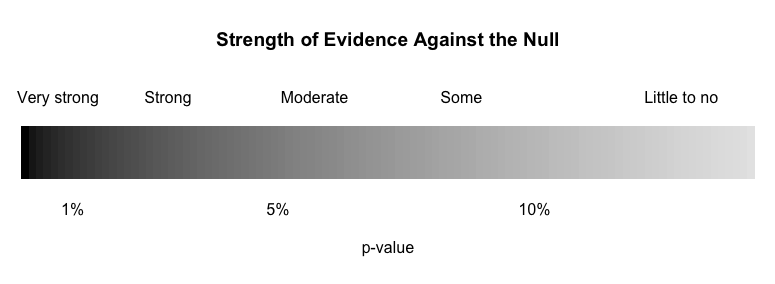
\includegraphics[width=0.9\linewidth]{images/soe_gradient_grayscale} \end{center}

\hypertarget{interpret-the-p-value}{%
\subsubsection*{Interpret the p-value}\label{interpret-the-p-value}}
\addcontentsline{toc}{subsubsection}{Interpret the p-value}

The p-value measures the probability that we observe a sample proportion as extreme as what was seen in the data or more extreme (matching the direction of the Ha) IF the null hypothesis is true.

\begin{enumerate}
\def\labelenumi{\arabic{enumi}.}
\setcounter{enumi}{9}
\tightlist
\item
  What did we assume to create the null distribution?
\end{enumerate}

\vspace{1in}

\begin{enumerate}
\def\labelenumi{\arabic{enumi}.}
\setcounter{enumi}{10}
\tightlist
\item
  What value did we compare to the null distribution to find the p-value?
\end{enumerate}

\vspace{0.3in}

\begin{enumerate}
\def\labelenumi{\arabic{enumi}.}
\setcounter{enumi}{11}
\item
  What direction did we count simulations from the statistic?
  \vspace{0.3in}
\item
  Fill in the blanks below to interpret the p-value.
\end{enumerate}

\setstretch{1.5}

We would observe a sample proportion of (value of the sample proportion )\hrulefill  

or (greater, less, more extreme) \hrulefill   

with a probability of (value of p-value) \hrulefill  

IF we assume (\(H_0\) in context) \hrulefill.

\setstretch{1}
\vspace{12pt}

\hypertarget{communicate-the-results-and-answer-the-research-question}{%
\subsubsection*{Communicate the results and answer the research question}\label{communicate-the-results-and-answer-the-research-question}}
\addcontentsline{toc}{subsubsection}{Communicate the results and answer the research question}

When we write a conclusion we answer the research question by stating how much evidence there is for the alternative hypothesis.

\begin{enumerate}
\def\labelenumi{\arabic{enumi}.}
\setcounter{enumi}{13}
\tightlist
\item
  Write a conclusion in context of the study. How much evidence does the data provide in support of the alternative hypothesis?
\end{enumerate}

\vspace{1in}

\hypertarget{take-home-messages-9}{%
\subsection{Take-home messages}\label{take-home-messages-9}}

\begin{enumerate}
\def\labelenumi{\arabic{enumi}.}
\item
  The null distribution is created based on the assumption the null hypothesis is true. We compare the sample statistic to the distribution to find the likelihood of observing this statistic.
\item
  The p-value measures the probability of observing the sample statistic or more extreme (in direction of the alternative hypothesis) is the null hypothesis is true.
\end{enumerate}

\hypertarget{additional-notes-8}{%
\subsection{Additional notes}\label{additional-notes-8}}

Use this space to summarize your thoughts and take additional notes on today's activity and material covered.

\newpage

\hypertarget{week-6-lab-helper-hinderer-simulation-based-confidence-interval}{%
\section{Week 6 Lab: Helper-Hinderer --- Simulation-based Confidence Interval}\label{week-6-lab-helper-hinderer-simulation-based-confidence-interval}}

\setstretch{1}

\hypertarget{learning-outcomes-11}{%
\subsection{Learning outcomes}\label{learning-outcomes-11}}

\begin{itemize}
\item
  Use bootstrapping to find a confidence interval for a single proportion.
\item
  Interpret a confidence interval for a single proportion.
\end{itemize}

\hypertarget{terminology-review-9}{%
\subsection{Terminology review}\label{terminology-review-9}}

In today's activity, we will introduce simulation-based confidence intervals for a single proportion. Some terms covered in this activity are:

\begin{itemize}
\item
  Parameter of interest
\item
  Bootstrapping
\item
  Confidence interval
\end{itemize}

To review these concepts, see Chapters 10 \& 14 in your textbook.

\hypertarget{helper-hinderer-2}{%
\subsection{Helper-Hinderer}\label{helper-hinderer-2}}

In the last class, we found very strong evidence that the true proportion of infants who will choose the helper character is greater than 0.5. But what \emph{is} the true proportion of infants who will choose the helper character? We will use this same study to estimate this parameter of interest by creating a confidence interval.

As a reminder: Do young children know the difference between helpful and unhelpful behavior? A study by Hamblin, Wynn, and Bloom reported in Nature (Hamblin, Wynn, and Bloom 2007) was intended to check young kids' feelings about helpful and non-helpful behavior. Non-verbal infants ages 6 to 10 months were shown short videos with different shapes either helping or hindering the climber. Researchers were hoping to assess: Are infants more likely to preferentially choose the helper toy over the hinderer toy? In the study, of the 16 infants age 6 to 10 months, 14 chose the \emph{helper} toy and 2 chose the \emph{hinderer} toy.

A \textbf{point estimate} (our observed statistic) provides a single plausible value for a parameter. However, a point estimate is rarely perfect; usually there is some error in the estimate. In addition to supplying a point estimate of a parameter, a next logical step would be to provide a plausible \emph{range} of values for the parameter. This plausible range of values for the population parameter is called an \textbf{interval estimate} or \textbf{confidence interval}.

\hypertarget{activity-intro}{%
\subsubsection*{Activity intro}\label{activity-intro}}
\addcontentsline{toc}{subsubsection}{Activity intro}

\begin{enumerate}
\def\labelenumi{\arabic{enumi}.}
\tightlist
\item
  What is the value of the point estimate?
\end{enumerate}

\vspace{0.3in}

\begin{enumerate}
\def\labelenumi{\arabic{enumi}.}
\setcounter{enumi}{1}
\tightlist
\item
  If we took another random sample of 16 infants, would we get the exact same point estimate? Explain why or why not.
\end{enumerate}

\vspace{0.5in}

In today's activity, we will use bootstrapping to find a 95\% confidence interval for \(\pi\), the parameter of interest.

\begin{enumerate}
\def\labelenumi{\arabic{enumi}.}
\setcounter{enumi}{2}
\tightlist
\item
  In your own words, explain the bootstrapping process.
  \vspace{0.5in}
\end{enumerate}

\hypertarget{use-statistical-analysis-methods-to-draw-inferences-from-the-data-1}{%
\subsubsection*{Use statistical analysis methods to draw inferences from the data}\label{use-statistical-analysis-methods-to-draw-inferences-from-the-data-1}}
\addcontentsline{toc}{subsubsection}{Use statistical analysis methods to draw inferences from the data}

\begin{enumerate}
\def\labelenumi{\arabic{enumi}.}
\setcounter{enumi}{3}
\tightlist
\item
  Write out the parameter of interest for this study in words. \emph{Hint: this is the same as in Activity 6A.}
\end{enumerate}

\vspace{0.5in}

To use the computer simulation to create a bootstrap distribution, we will need to enter the

\begin{itemize}
\tightlist
\item
  ``sample size'' (the number of observational units or cases in the sample),
\item
  ``number of successes'' (the number of cases that choose the helper character),
\item
  ``number of repetitions'' (the number of samples to be generated), and
\item
  the ``confidence level'' (which level of confidence are we using to create the confidence interval).
\end{itemize}

\begin{enumerate}
\def\labelenumi{\arabic{enumi}.}
\setcounter{enumi}{4}
\tightlist
\item
  What values should be entered for each of the following into the simulation to create the bootstrap distribution of sample proportions to find a 95\% confidence interval?
  \vspace{1mm}
\end{enumerate}

\begin{itemize}
\tightlist
\item
  Sample size:
\end{itemize}

\vspace{.1in}

\begin{itemize}
\tightlist
\item
  Number of successes:
\end{itemize}

\vspace{.1in}

\begin{itemize}
\tightlist
\item
  Number of repetitions:
\end{itemize}

\vspace{.1in}

\begin{itemize}
\tightlist
\item
  Confidence level (as a decimal):
\end{itemize}

\vspace{.1in}

We will use the \texttt{one\_proportion\_bootstrap\_CI()} function in R (in the \texttt{catstats} package) to simulate the bootstrap distribution of sample proportions and calculate a confidence interval. Using the provided R script file, fill in the values/words for each \texttt{xx} with your answers from question 5 in the one proportion bootstrap confidence interval (CI) code to create a bootstrap distribution with 1000 simulations. Then highlight and run lines 1--7.

\begin{Shaded}
\begin{Highlighting}[]
\FunctionTok{one\_proportion\_bootstrap\_CI}\NormalTok{(}\AttributeTok{sample\_size =}\NormalTok{ xx, }\CommentTok{\# Sample size}
                    \AttributeTok{number\_successes =}\NormalTok{ xx, }\CommentTok{\# Observed number of successes}
                    \AttributeTok{number\_repetitions =} \DecValTok{1000}\NormalTok{, }\CommentTok{\# Number of bootstrap samples to use}
                    \AttributeTok{confidence\_level =} \FloatTok{0.95}\NormalTok{) }\CommentTok{\# Confidence level as a decimal}
\end{Highlighting}
\end{Shaded}

\newpage

\begin{enumerate}
\def\labelenumi{\arabic{enumi}.}
\setcounter{enumi}{5}
\tightlist
\item
  Sketch the bootstrap distribution created below.
\end{enumerate}

\vspace{1.8in}

\begin{enumerate}
\def\labelenumi{\arabic{enumi}.}
\setcounter{enumi}{6}
\item
  What is the value at the center of this bootstrap distribution? Why does this make sense?
  \vspace{.8in}
\item
  \textbf{Explain why the two vertical lines are at the 2.5th percentile and the 97.5th percentile.}
\end{enumerate}

\vspace{.7in}

\begin{enumerate}
\def\labelenumi{\arabic{enumi}.}
\setcounter{enumi}{8}
\tightlist
\item
  Report the 95\% bootstrapped confidence interval for \(\pi\). Use interval notation: (lower value, upper value).
\end{enumerate}

\vspace{0.2in}

\begin{enumerate}
\def\labelenumi{\arabic{enumi}.}
\setcounter{enumi}{9}
\tightlist
\item
  \textbf{Interpret the 95\% confidence interval in context.}
\end{enumerate}

\vspace{.7in}

\hypertarget{communicate-the-results-and-answer-the-research-question-1}{%
\subsubsection*{Communicate the results and answer the research question}\label{communicate-the-results-and-answer-the-research-question-1}}
\addcontentsline{toc}{subsubsection}{Communicate the results and answer the research question}

\begin{enumerate}
\def\labelenumi{\arabic{enumi}.}
\setcounter{enumi}{10}
\tightlist
\item
  \textbf{Is the value 0.5 (the null value) in the 95\% confidence interval?}
\end{enumerate}

\vspace{.2in}

~~~\textbf{Explain how this indicates that the p-value provides strong evidence against the null.}

\newpage

\hypertarget{effect-of-confidence-level}{%
\subsubsection*{Effect of confidence level}\label{effect-of-confidence-level}}
\addcontentsline{toc}{subsubsection}{Effect of confidence level}

\begin{enumerate}
\def\labelenumi{\arabic{enumi}.}
\setcounter{enumi}{11}
\tightlist
\item
  Suppose instead of finding a 95\% confidence interval, we found a 90\% confidence interval. Would you expect the 90\% confidence interval to be narrower or wider? Explain your answer.
\end{enumerate}

\vspace{0.4in}

\begin{enumerate}
\def\labelenumi{\arabic{enumi}.}
\setcounter{enumi}{12}
\tightlist
\item
  The following R code produced the bootstrap distribution with 1000 simulations that follows. Circle the value that changed in the code.
\end{enumerate}

\begin{Shaded}
\begin{Highlighting}[]
\FunctionTok{one\_proportion\_bootstrap\_CI}\NormalTok{(}\AttributeTok{sample\_size =} \DecValTok{16}\NormalTok{, }\CommentTok{\# Sample size}
                    \AttributeTok{number\_successes =} \DecValTok{14}\NormalTok{, }\CommentTok{\# Observed number of successes}
                    \AttributeTok{number\_repetitions =} \DecValTok{1000}\NormalTok{, }\CommentTok{\# Number of bootstrap samples to use}
                    \AttributeTok{confidence\_level =} \FloatTok{0.90}\NormalTok{) }\CommentTok{\# Confidence level as a decimal}
\end{Highlighting}
\end{Shaded}

\begin{center}\includegraphics[width=0.7\linewidth]{06-L04-inference-1cat_CI-simulation_files/figure-latex/unnamed-chunk-2-1} \end{center}

\begin{enumerate}
\def\labelenumi{\arabic{enumi}.}
\setcounter{enumi}{13}
\tightlist
\item
  Report both the 95\% confidence interval (question 9) and the 90\% confidence interval (question 13). Is the 90\% confidence interval narrower or wider than the 95\% confidence interval?
\end{enumerate}

\vspace{0.5in}

\begin{enumerate}
\def\labelenumi{\arabic{enumi}.}
\setcounter{enumi}{14}
\tightlist
\item
  Explain why the upper value of the confidence interval is truncated at 1.
\end{enumerate}

\vspace{0.5in}

\newpage

\setstretch{1.5}

\begin{enumerate}
\def\labelenumi{\arabic{enumi}.}
\setcounter{enumi}{15}
\tightlist
\item
  Fill in the blanks below to write a paragraph summarizing the results of the study as if writing a press release. \textbf{Complete your group's paragraph on Gradescope.}\\
  Researchers were interested if infants observe social cues and would be more likely to choose the helper toy over the hinderer toy. In a sample of (sample size) \_\_\_\_\_\_\_\_\_\_\_\_\_infants, (number of successes) \_\_\_\_\_\_\_\_\_\_\_\_\_\_\_chose the helper toy. A simulation null distribution with 1000 simulations was created in RStudio. The p-value was found by calculating the proportion of simulations in the null distribution at the sample statistic of 0.875 and greater. This resulted in a p-value of (value of p-value)\_\_\_\_\_\_\_\_\_\_\_\_\_\_\_. We would observe a sample proportion of (value of the sample proportion) \_\_\_\_\_\_\_\_\_\_\_\_\_\_\_\_\_\_\_\_\_\_ or (greater, less, more extreme) \_\_\_\_\_\_\_\_\_\_\_\_\_\_\_\_\_\_\_\_\_ with a probability of (value of p-value)\_\_\_\_\_\_\_\_\_\_\_\_\_\_\_\_\_\_\_\\
  IF we assume (\(H_0\) in context) \_\_\_\_\_\_\_\_\_\_\_\_\_\_\_\_\_\_\_\_\_\_\_\_\_\_\_\_\_\_\_\_\_\_\_\_\_\_\_\_\_\_\_\_.
  Based on this p-value, there is (very strong/little to no) \_\_\_\_\_\_\_\_\_\_\_\_\_\_\_\_\_\_\_\_\_\_ evidence that the (sample/true)\_\_\_\_\_\_\_\_\_\_\_\_\_\_\_\_\_\_\_\_\_ proportion of infants age 6 to 10 months who will choose the helper toy is (greater than, less than, not equal to) \_\_\_\_\_\_\_\_\_\_\_\_\_\_\_\_\_\_\_\_\_ 0.5. In addition, a 95\% confidence interval was found for the parameter of interest. We are 95\% confident that the (true/sample)\_\_\_\_\_\_\_\_\_\_\_\_\_\_\_\_\_\_\_\_\_\_\_\_\_ proportion of infants age 6 to 10 months who will choose the helper toy is between (lower value)\_\_\_\_\_\_\_\_\_\_\_\_\_\_\_\_ and (upper value)\_\_\_\_\_\_\_\_\_\_\_\_\_\_\_\_\_\_\_\_. The results of this study can be generalized to (all infants age 6 to 10 months/infants similar to those in this study)\_\_\_\_\_\_\_\_\_\_\_\_\_\_\_\_\_\_\_\_\_\_\_\_\_\_\_ as the researchers (did/did not)\_\_\_\_\_\_\_\_\_\_\_\_\_\_\_\_\_\_\_\_\_ select a random sample.
\end{enumerate}

\setstretch{1}

\hypertarget{take-home-messages-10}{%
\subsection{Take-home messages}\label{take-home-messages-10}}

\begin{enumerate}
\def\labelenumi{\arabic{enumi}.}
\item
  The goal in a hypothesis test is to assess the strength of evidence for an effect, while the goal in creating a confidence interval is to determine how large the effect is. A \textbf{confidence interval} is a range of \emph{plausible} values for the parameter of interest.
\item
  A confidence interval is built around the point estimate or observed calculated statistic from the sample. This means that the sample statistic is always the center of the confidence interval. A confidence interval includes a measure of sample to sample variability represented by the \textbf{margin of error}.
\item
  In simulation-based methods (bootstrapping), a simulated distribution of possible sample statistics is created showing the possible sample-to-sample variability. Then we find the middle \(X\) percent of the distribution around the sample statistic using the percentile method to give the range of values for the confidence interval. This shows us that we are \(X\)\% confident that the parameter is within this range, where \(X\) represents the level of confidence.
\item
  When the null value is within the confidence interval, it is a plausible value for the parameter of interest; thus, we would find a larger p-value for a hypothesis test of that null value. Conversely, if the null value is NOT within the confidence interval, we would find a small p-value for the hypothesis test and strong evidence against this null hypothesis.
\item
  To create one simulated sample on the bootstrap distribution for a sample proportion, label \(n\) cards with the original responses. Draw with replacement \(n\) times. Calculate and plot the resampled proportion of successes.
\end{enumerate}

\hypertarget{additional-notes-9}{%
\subsection{Additional notes}\label{additional-notes-9}}

Use this space to summarize your thoughts and take additional notes on today's activity and material covered.

\newpage

\hypertarget{inference-for-a-single-categorical-variable-theory-based-methods-errors-and-power}{%
\chapter{Inference for a Single Categorical Variable: Theory-based Methods + Errors and Power}\label{inference-for-a-single-categorical-variable-theory-based-methods-errors-and-power}}

\hypertarget{week-7-reading-guide-categorical-inference}{%
\section{Week 7 Reading Guide: Categorical Inference}\label{week-7-reading-guide-categorical-inference}}

\hypertarget{chapter-11-inference-with-mathematical-models}{%
\subsection*{Chapter 11 (Inference with mathematical models)}\label{chapter-11-inference-with-mathematical-models}}
\addcontentsline{toc}{subsection}{Chapter 11 (Inference with mathematical models)}

\setstretch{1}

\textbf{Videos}

\begin{itemize}
\tightlist
\item
  Chapter11
\end{itemize}

\setstretch{1.25}

\hypertarget{reminders-from-previous-sections-4}{%
\subsubsection*{Reminders from previous sections}\label{reminders-from-previous-sections-4}}
\addcontentsline{toc}{subsubsection}{Reminders from previous sections}

\(n_1\)= sample size of group 1

\(n_2\) = sample size of group 2

\(\overline{x}\) = sample mean

\(s\) = sample standard deviation

\(\mu\) = population mean

\(\sigma\) = population standard deviation

General steps of a hypothesis test:

\begin{enumerate}
\def\labelenumi{\arabic{enumi}.}
\item
  Frame the research question in terms of hypotheses.
\item
  Collect and summarize data using a test statistic.
\item
  Assume the null hypothesis is true, and simulate or mathematically model a null distribution for the test statistic.
\item
  Compare the observed test statistic to the null distribution to calculate a p-value.
\item
  Make a conclusion based on the p-value and write the conclusion in context.
\end{enumerate}

Parameter: a value summarizing a variable(s) for a population.

Statistic: a value summarizing a variable(s) for a sample.

Hypothesis test: a process to determine how strong the evidence of an effect is. Also called a `significance test'.

Simulation-based method: Simulate lots of samples of size \(n\) under assumption of the null hypothesis, then find the proportion of the simulations that are at least as extreme as the observed sample statistic.

Theory-based method: Develop a mathematical model for the sampling distribution of the statistic under the null hypothesis and use the model to calculate the probability of the observed sample statistic (or one more extreme) occurring.

Null hypothesis (\(H_0\)): the skeptical perspective; no difference; no change; no effect; random chance; what the researcher hopes to prove is \textbf{wrong}.

Alternative hypothesis (\(H_A\)): the new perspective; a difference/increase/decrease; an effect; not random chance; what the researcher hopes to prove is \textbf{correct}.

Null value: the value of the parameter when we assume the null hypothesis is true (labeled as \(parameter_0\)).

P-value: probability of seeing the observed sample data, or something more extreme, assuming the null hypothesis is true.

\(\implies\) Lower the p-value the stronger the evidence AGAINST the null hypothesis and FOR the alternative hypothesis.

Significance level (\(\alpha\)): a threshold used to determine if a p-value provides enough evidence to reject the null hypothesis or not.

\rgi Common levels of \(\alpha\) include 0.01, 0.05, and 0.10.

Statistically significant: results are considered statistically significant if the p-value is below the significance level.

Confidence interval: a process to determine how large an effect is; a range of plausible values for the parameter. Also called `estimation'.

\hypertarget{vocabulary-12}{%
\subsubsection*{Vocabulary}\label{vocabulary-12}}
\addcontentsline{toc}{subsubsection}{Vocabulary}

Central Limit Theorem:
\rgs

Sampling distribution:
\rgs

Normal distribution (Also known as: normal curve, normal model, Gaussian distribution):
\rgs

\rgi Notation:
\rgs

Standard normal distribution:
\rgs

\rgi Notation:
\rgs

Z-score:
\rgs

\(X\)th percentile:
\rgs

68-95-99.7 rule:
\rgs

Standard error of a statistic:
\rgs

Standard deviation of a statistic:
\rgs

Margin of error:
\rgs

\hypertarget{notes-17}{%
\subsubsection*{Notes}\label{notes-17}}
\addcontentsline{toc}{subsubsection}{Notes}

The two general conditions for the sampling distribution for a sample proportion (or difference in sample proportions) to be approximately normally distributed are:

\rgi 1)
\rgs

\rgi 2)
\rgs

Interpretation of a Z-score:
\rgs

True or False: The more unusual observation will be the observation with the largest Z-score.

Approximately what percent of a normal distribution is in the interval

\rgi (mean -- standard deviation, mean + standard deviation):
\rgs

\rgi (mean -- 2\(\times\)(standard deviation), mean + 2\(\times\)(standard deviation)):
\rgs

\rgi (mean -- 3\(\times\)(standard deviation), mean + 3\(\times\)(standard deviation)):
\rgs

Given a mean and standard deviation, what function in R would help us find the percent of the normal distribution above (or below) a specific value?
\rgs

Given a mean and standard deviation, what function in R would help us find the value at a given percentile?
\rgs

How is the standard deviation of a statistic (\(SD(statistic)\)) different from the standard error of a statistic (\(SE(statistic)\))?
\rgs

How is the standard deviation of a statistic (\(SD(statistic)\)) different from the standard deviation of a sample (\(s\))?
\rgs

\hypertarget{formulas}{%
\subsubsection*{Formulas}\label{formulas}}
\addcontentsline{toc}{subsubsection}{Formulas}

Z =
\rgs

\(SD(\hat{p})\) =
\rgs

General form of a theory-based confidence interval =
\rgs

General form for margin of error =
\rgs

\hypertarget{r-coding}{%
\subsection*{R coding}\label{r-coding}}
\addcontentsline{toc}{subsection}{R coding}

\hypertarget{calculating-normal-probabilities}{%
\paragraph*{Calculating normal probabilities}\label{calculating-normal-probabilities}}
\addcontentsline{toc}{paragraph}{Calculating normal probabilities}

When using the \texttt{pnorm()} R function, you will need to enter values for the arguments \texttt{mean}, \texttt{sd}, and \texttt{q} to match the question.

\begin{Shaded}
\begin{Highlighting}[]
\FunctionTok{pnorm}\NormalTok{(}\AttributeTok{mean =}\NormalTok{ mu, }\AttributeTok{sd =}\NormalTok{ sigma, }\AttributeTok{q =}\NormalTok{ x, }\AttributeTok{lower.tail =} \ConstantTok{TRUE}\NormalTok{)}
\end{Highlighting}
\end{Shaded}

This function will return the proportion of the N(\texttt{mu},\texttt{sigma}) distribution which is \emph{below} the value \texttt{x}.

Example: \texttt{pnorm(mean\ =\ 5,\ sd\ =\ 2,\ q\ =\ 3,\ lower.tail\ =\ TRUE)} will give us the proportion of a N(5,2) distribution which is below 3, which equals 0.159:

\begin{Shaded}
\begin{Highlighting}[]
\FunctionTok{pnorm}\NormalTok{(}\AttributeTok{mean =} \DecValTok{5}\NormalTok{, }\AttributeTok{sd =} \DecValTok{2}\NormalTok{, }\AttributeTok{q =} \DecValTok{3}\NormalTok{, }\AttributeTok{lower.tail =} \ConstantTok{TRUE}\NormalTok{)}
\CommentTok{\#\textgreater{} [1] 0.1586553}
\end{Highlighting}
\end{Shaded}

Changing to \texttt{lower.tail\ =\ FALSE} will give the proportion of the distribution which is \emph{above} the value \texttt{x}.

\begin{Shaded}
\begin{Highlighting}[]
\FunctionTok{pnorm}\NormalTok{(}\AttributeTok{mean =} \DecValTok{5}\NormalTok{, }\AttributeTok{sd =} \DecValTok{2}\NormalTok{, }\AttributeTok{q =} \DecValTok{3}\NormalTok{, }\AttributeTok{lower.tail =} \ConstantTok{FALSE}\NormalTok{)}
\CommentTok{\#\textgreater{} [1] 0.8413447}
\end{Highlighting}
\end{Shaded}

\hypertarget{displaying-normal-probabilities}{%
\paragraph*{Displaying normal probabilities}\label{displaying-normal-probabilities}}
\addcontentsline{toc}{paragraph}{Displaying normal probabilities}

When using the \texttt{normTail()} R function, you will need to enter values for the arguments \texttt{m}, \texttt{s}, and \texttt{L} (or \texttt{U}) to match the question.

\begin{Shaded}
\begin{Highlighting}[]
\FunctionTok{normTail}\NormalTok{(}\AttributeTok{m =}\NormalTok{ mu, }\AttributeTok{s =}\NormalTok{ sigma, }\AttributeTok{L =}\NormalTok{ x)}
\end{Highlighting}
\end{Shaded}

This function (in the \texttt{openintro} package) will plot a N(\texttt{mu}, \texttt{sigma}) distribution and shade the area that is below the value \texttt{x}.

Example: \texttt{normTail(m\ =\ 5,\ s\ =\ 2,\ L\ =\ 3)} creates the plot pictured below.

\begin{figure}

{\centering 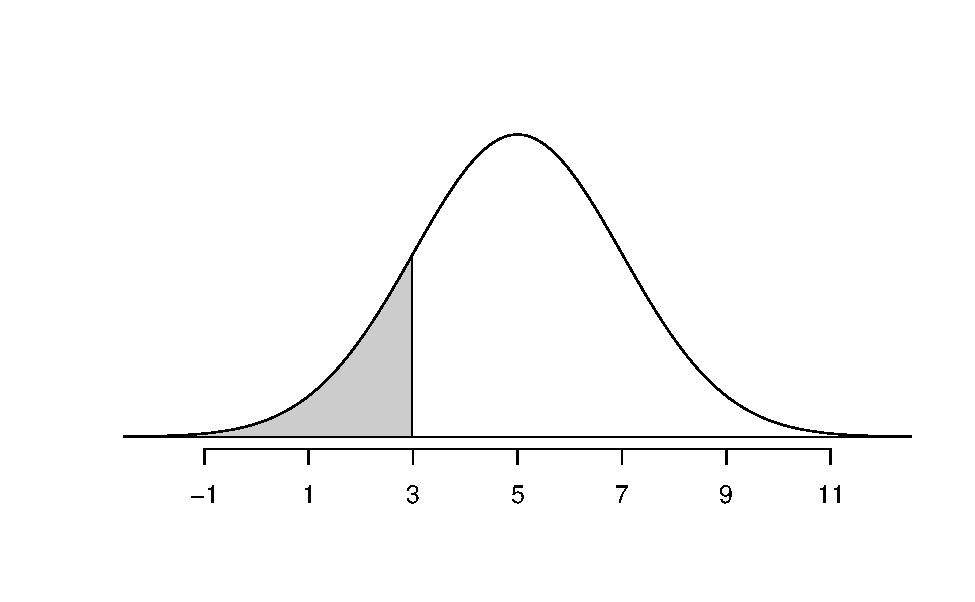
\includegraphics[width=0.6\linewidth]{07-RG-1cat_theory_files/figure-latex/normgt3-1} 

}

\end{figure}

Changing \texttt{L} to \texttt{U} will shade the area \emph{above} \texttt{x}.

Example: \texttt{normTail(m\ =\ 5,\ s\ =\ 2,\ U\ =\ 3)} plots a N(5,2) distribution with the area above 3 shaded.

\hypertarget{calculating-normal-percentiles}{%
\paragraph*{Calculating normal percentiles}\label{calculating-normal-percentiles}}
\addcontentsline{toc}{paragraph}{Calculating normal percentiles}

When using the \texttt{qnorm()} R function, you will need to enter values for the arguments \texttt{mean}, \texttt{sd}, and \texttt{p} to match the question.

\begin{Shaded}
\begin{Highlighting}[]
\FunctionTok{qnorm}\NormalTok{(}\AttributeTok{mean =}\NormalTok{ mu, }\AttributeTok{sd =}\NormalTok{ sigma, }\AttributeTok{p =}\NormalTok{ x, }\AttributeTok{lower.tail =} \ConstantTok{TRUE}\NormalTok{)}
\end{Highlighting}
\end{Shaded}

This function will return the value on the N(\texttt{mu}, \texttt{sigma}) distribution which has \texttt{x} area of the distribution \emph{below} it.

Example: \texttt{qnorm(mean\ =\ 5,\ sd\ =\ 2,\ p\ =\ 0.159,\ lower.tail\ =\ TRUE)} will give us the value on a N(5,2) distribution which has 0.159 (15.9\%) of the distribution below it, which equals 3 (from the R output above).

Changing to \texttt{lower.tail\ =\ FALSE} will give the value which has \texttt{x} area of the distribution \emph{above} it.

We would recommend you work through each of the examples in Section 5.2.4 using R.

\hypertarget{section-14.3-theory-based-inferential-methods-for-pi}{%
\subsection*{\texorpdfstring{Section 14.3 (Theory-based inferential methods for \(\pi\))}{Section 14.3 (Theory-based inferential methods for \textbackslash pi)}}\label{section-14.3-theory-based-inferential-methods-for-pi}}
\addcontentsline{toc}{subsection}{Section 14.3 (Theory-based inferential methods for \(\pi\))}

\setstretch{1}

\textbf{Videos}

\begin{itemize}
\tightlist
\item
  14.3TheoryTests
\item
  14.3TheoryIntervals
\end{itemize}

\setstretch{1.25}

\hypertarget{vocabulary-13}{%
\subsubsection*{Vocabulary}\label{vocabulary-13}}
\addcontentsline{toc}{subsubsection}{Vocabulary}

\hypertarget{reminders-from-previous-sections-5}{%
\subsubsection*{Reminders from previous sections}\label{reminders-from-previous-sections-5}}
\addcontentsline{toc}{subsubsection}{Reminders from previous sections}

\(n\) = sample size

\(\hat{p}\) = sample proportion

\(\pi\) = population proportion

General steps of a hypothesis test:

\begin{enumerate}
\def\labelenumi{\arabic{enumi}.}
\item
  Frame the research question in terms of hypotheses.
\item
  Collect and summarize data using a test statistic.
\item
  Assume the null hypothesis is true, and simulate or mathematically model a null distribution for the test statistic.
\item
  Compare the observed test statistic to the null distribution to calculate a p-value.
\item
  Make a conclusion based on the p-value and write the conclusion in context.
\end{enumerate}

Parameter: a value summarizing a variable(s) for a population.

Statistic: a value summarizing a variable(s) for a sample.

Sampling distribution: plot of statistics from 1000s of samples of the same size taken from the same population.

Standard deviation of a statistic: the variability of statistics from 1000s of samples; how far, on average, each statistic is from the true value of the parameter.

Standard error of a statistic: estimated standard deviation of a statistic.

Hypothesis test: a process to determine how strong the evidence of an effect is.

\rgi Also called a `significance test'.

Theory-based method: Develop a mathematical model for the sampling distribution of the statistic under the null hypothesis and use the model to calculate the probability of the observed sample statistic (or one more extreme) occurring.

Null hypothesis (\(H_0\)): the skeptical perspective; no difference; no change; no effect; random chance; what the researcher hopes to prove is \textbf{wrong}.

Alternative hypothesis (\(H_A\)): the new perspective; a difference/increase/decrease; an effect; not random chance; what the researcher hopes to prove is \textbf{correct}.

P-value: probability of seeing the observed sample data, or something more extreme, assuming the null hypothesis is true.

\(\implies\) Lower the p-value the stronger the evidence AGAINST the null hypothesis and FOR the alternative hypothesis.

Decision: a determination of whether to `reject' or `fail to reject' a null hypothesis based on a p-value and a pre-set level of significance.

Significance level (\(\alpha\)): a threshold used to determine if a p-value provides enough evidence to reject the null hypothesis or not.

\rgi Common levels of \(\alpha\) include 0.01, 0.05, and 0.10.

Statistically significant: results are considered statistically significant if the p-value is below the significance level.

Central Limit Theorem: For large sample sizes, the sampling distribution of a sample proportion (or mean) will be approximately normal (bell-shaped and symmetric).

Confidence interval: a process to determine how large an effect is; a range of plausible values for the parameter; also called `estimation'.

Margin of error: the value that is added to and subtracted from the sample statistic to create a confidence interval; half the width of a confidence interval.

\hypertarget{vocabulary-14}{%
\subsubsection*{Vocabulary}\label{vocabulary-14}}
\addcontentsline{toc}{subsubsection}{Vocabulary}

Null standard error:
\rgs

Standardized statistic:
\rgs

Confidence level:
\rgs

\hypertarget{notes-18}{%
\subsubsection*{Notes}\label{notes-18}}
\addcontentsline{toc}{subsubsection}{Notes}

Conditions for the Central Limit Theorem to apply (for the sampling distribution of \(\hat{p}\) to be approximately normal)

\rgi Independence:
\rgs

\rgi \rgi Checked by:
\rgs

\rgi Success-failure condition:
\rgs

\rgi \rgi Checked by:
\rgs

How can we determine the value of \(z^⋆\) to use as the multiplier in a confidence interval?
\rgs

\rgi In R, use \texttt{qnorm(mean\ =\ \_\_,\ sd\ =\ \_\_,\ p\ =\ \_\_)}.

Select one answer in each set of parentheses: The higher the confidence level, the (larger/smaller) the multiplier, meaning the confidence interval will be (wider/narrower).

If the success-failure condition for the Central Limit Theorem is not met, what is the appropriate method of analysis? Select one:
\rgi A. Theory-based approach
\rgi B. Simulation based approach.

\hypertarget{formulas-1}{%
\subsubsection*{Formulas}\label{formulas-1}}
\addcontentsline{toc}{subsubsection}{Formulas}

\(SD(\hat{p})\) =
\rgs

Null standard error of the sample proportion:

\(SE_0(\hat{p})\) =
\rgs

Standardized statistic (in this case, standardized sample proportion):

\(Z\) =
\rgs

Standard error of the sample proportion when we do not assume the null hypothesis is true:

\(SE(\hat{p})\) =
\rgs

Theory-based confidence interval for a sample proportion:
\rgs

Margin of error of a confidence interval for a sample proportion:
\rgs

\hypertarget{example-payday-loans}{%
\subsubsection*{Example: Payday loans}\label{example-payday-loans}}
\addcontentsline{toc}{subsubsection}{Example: Payday loans}

\begin{enumerate}
\def\labelenumi{\arabic{enumi}.}
\item
  What is the parameter representing in the context of this problem? What notation would be used to represent this parameter?
  \rgs
  \rgs
\item
  Write the null and alternative hypotheses in words.
  \rgs
  \rgs
\item
  Write the null and alternative hypotheses in notation.
  \rgs
\item
  Are the conditions met to use theoretical methods to analyze these data? Show your calculations to justify your answer.
  \rgs
  \rgs
\item
  Calculate the null standard error of the sample proportion.
  \rgs
  \rgs
\item
  What is the sample statistic presented in this example? What notation would be used to represent this value?
  \rgs
\item
  Calculate the standardized sample proportion (standardized statistic).
  \rgs
  \rgs
\item
  How can we calculate a p-value from the normal distribution for this example?
  \rgs
  \rgs
\item
  What was the p-value of the test?
  \rgs
\item
  What conclusion should the researcher make?
  \rgs
  \rgs
\item
  Are the results in this example statistically significant? Justify your answer.
  \rgs
\item
  Calculate the standard error of the sample proportion when we do not assume the null hypothesis is true.
  \rgs
  \rgs
\item
  Calculate the margin of error for a 95\% confidence interval for \(\pi\) using 1.96 as the multiplier.
  \rgs
  \rgs
\item
  Calculate a 95\% confidence interval for \(\pi\) using your margin of error calculated above.
  \rgs
  \rgs
\item
  Interpret the 95\% confidence interval provided in the textbook.
  \rgs
  \rgs
\item
  Does the 95\% confidence interval support the same conclusion as the p-value from the hypothesis test? Justify your answer.
  \rgs
\end{enumerate}

\hypertarget{chapter-12-errors-power-and-practical-importance}{%
\subsection*{Chapter 12 (Errors, power, and practical importance)}\label{chapter-12-errors-power-and-practical-importance}}
\addcontentsline{toc}{subsection}{Chapter 12 (Errors, power, and practical importance)}

\setstretch{1}

\textbf{Videos}

\begin{itemize}
\tightlist
\item
  Chapter12
\end{itemize}

\setstretch{1.25}

\hypertarget{reminders-from-previous-sections-6}{%
\subsubsection*{Reminders from previous sections}\label{reminders-from-previous-sections-6}}
\addcontentsline{toc}{subsubsection}{Reminders from previous sections}

Significance level (\(\alpha\)): a threshold used to determine if a p-value provides enough evidence to reject the null hypothesis or not.

\rgi Common levels of \(\alpha\) include 0.01, 0.05, and 0.10.

Statistically significant: results are considered statistically significant if the p-value is below the significance level.

\hypertarget{vocabulary-15}{%
\subsubsection*{Vocabulary}\label{vocabulary-15}}
\addcontentsline{toc}{subsubsection}{Vocabulary}

Decision:

\rgs

\begin{itemize}
\item
  If the p-value is small (less than or equal to the significance level), the decision will be to \_\_\_\_\_\_\_\_\_\_ the null hypothesis.
\item
  If the p-value is large (greater than the significance level), the decision will be to \_\_\_\_\_\_\_\_\_\_ the null hypothesis.
\end{itemize}

Type 1 error:
\rgs

Type 2 error:
\rgs

Confirmation bias:
\rgs

One-sided hypothesis tests:
\rgs

Two-sided hypothesis tests:
\rgs

Power:
\rgs

Practical importance:
\rgs

\hypertarget{notes-19}{%
\subsubsection*{Notes}\label{notes-19}}
\addcontentsline{toc}{subsubsection}{Notes}

Fill in the following table with whether the decision was correct or not, and if not, what type of error was made.

\begin{center}
\begin{tabular}{|p{2in}|p{2in}|p{2in}|}
\hline
 & \multicolumn{2}{|c|}{\textbf{Test conclusion (based on data)}} \\ \hline
 \textbf{Truth (unknown)} & Reject null hyp. & Fail to reject null hyp. \\ \hline
 $H_0$ is true && \\ 
   & & \\ 
   & & \\ \hline
 $H_A$ is true ($H_0$ is false)  && \\ 
   & & \\ 
   & & \\ \hline
\end{tabular}
\end{center}

\rgs

How are the significance level and type I error rate related?
\rgs

How are the significance level and type II error rate related?
\rgs

Explain the differences between a one-sided and two-sided hypothesis test.
\vspace{1mm}

\rgi How will the research questions differ?
\rgs

\rgi How will the notation in the alternative hypothesis differ?
\rgs

\rgi How does the p-value calculation differ?
\rgs

How does the p-value in a two-sided test compare to the p-value in a one-sided test?
\rgs

Should the default in research be a one-sided or two-sided hypothesis test? Explain why.
\rgs
\rgs

After collecting data, a researcher decides to change from a two-sided test to a one-sided test. Why is this a bad idea?

\begin{enumerate}
\def\labelenumi{\arabic{enumi}.}
\item
  It \_\_\_\_\_\_\_\_\_\_\_\_ (increases/decreases) the chance of a type I error.
\item
  This can result in \_\_\_\_\_\_\_\_\_\_\_\_\_\_\_\_\_\_\_\_\_\_\_\_.
  \rgs
\end{enumerate}

How are power and type I error rate related?
\rgs

How are power and type II error rate related?
\rgs

How can we increase the power of a test?

\begin{enumerate}
\def\labelenumi{\arabic{enumi}.}
\item
  \_\_\_\_\_\_\_\_ (Increase/Decrease) the significance level
  \rgs
\item
  \_\_\_\_\_\_\_\_ (Increase/Decrease) the sample size
  \rgs
\item
  Change from a \_\_\_ (one/two)-sided to a \_\_\_ (one/two)-sided test
  \rgs
\item
  Have a \_\_\_\_\_\_\_\_ (larger/smaller) standard deviation of the statistic
  \rgs
\item
  Have the alternative parameter value \_\_\_\_\_\_\_ (closer/farther) from the null value
  \rgs
\end{enumerate}

Results are likely to be statistically significant (but may not be practically important) if the sample size is \_\_\_\_\_\_\_\_\_\_(large/small).
\rgs

Results are unlikely to be statistically significant (but may be practically important) if the sample size is \_\_\_\_\_\_\_\_\_\_(large/small).
\rgs

\hypertarget{examples}{%
\subsubsection*{Examples:}\label{examples}}
\addcontentsline{toc}{subsubsection}{Examples:}

\begin{enumerate}
\def\labelenumi{\arabic{enumi}.}
\tightlist
\item
  In the Martian Alphabet study section 9.1 of the textbook,
\end{enumerate}

\rgi a. What was the p-value of the test?
\rgs

\rgi b. At the 5\% significance level, what decision would you make?
\rgs

\rgi c.~What type of error might have occurred in these data?
\rgs

\rgi d.~Interpret that error in the context of the problem.
\rgs
\rgs

\begin{enumerate}
\def\labelenumi{\arabic{enumi}.}
\setcounter{enumi}{1}
\tightlist
\item
  In the Medical Consultant study in section 10.1 of the textbook,
\end{enumerate}

\rgi a. What was the p-value of the test?
\rgs

\rgi b. At the 5\% significance level, what decision would you make?
\rgs

\rgi c.~What type of error might have occurred in these data?
\rgs

\rgi d.~Interpret that error in the context of the problem.
\rgs
\rgs

\begin{enumerate}
\def\labelenumi{\arabic{enumi}.}
\setcounter{enumi}{2}
\tightlist
\item
  In the Payday Loans study section 14.3 of the textbook,
\end{enumerate}

\rgi a. What was the p-value of the test?
\rgs

\rgi b. At the 5\% significance level, what decision would you make?
\rgs

\rgi c.~What type of error might have occurred in these data?
\rgs

\rgi d.~Interpret that error in the context of the problem.
\rgs

\newpage

\hypertarget{activity-7a-handedness-of-male-boxers-theory-based-methods}{%
\section{Activity 7A: Handedness of Male Boxers --- Theory-based Methods}\label{activity-7a-handedness-of-male-boxers-theory-based-methods}}

\setstretch{1}

\hypertarget{learning-outcomes-12}{%
\subsection{Learning outcomes}\label{learning-outcomes-12}}

\begin{itemize}
\item
  Describe and perform a theory-based hypothesis test for a single proportion.
\item
  Check the appropriate conditions to use a theory-based hypothesis test.
\item
  Calculate and interpret the standardized sample proportion.
\item
  Interpret and evaluate a p-value for a theory-based hypothesis test for a single proportion.
\item
  Use the normal distribution to find the p-value.
\end{itemize}

\hypertarget{terminology-review-10}{%
\subsection{Terminology review}\label{terminology-review-10}}

In today's activity, we will introduce theory-based hypothesis tests for a single categorical variable. Some terms covered in this activity are:

\begin{itemize}
\item
  Parameter of interest
\item
  Standardized Statistic
\item
  Normal distribution
\item
  p-value
\end{itemize}

To review these concepts, see Chapters 11 \& 14 in your textbook.

Activities 6A, 6B, and the Week 6 Lab covered simulation-based methods for hypothesis tests involving a single categorical variable. This activity covers theory-based methods for testing a single categorical variable.

\hypertarget{handedness-of-male-boxers}{%
\subsection{Handedness of male boxers}\label{handedness-of-male-boxers}}

Left-handedness is a trait that is found in about 10\% of the general population. Past studies have shown that left-handed men are over-represented among professional boxers (Richardson and Gilman 2019). The fighting claim states that left-handed men have an advantage in competition. In this random sample of 500 male professional boxers, we want to see if there is an over-prevalence of left-handed fighters. In the sample of 500 male boxers, 81 were left-handed.

\begin{Shaded}
\begin{Highlighting}[]
 \CommentTok{\# Read in data set}
\NormalTok{boxers }\OtherTok{\textless{}{-}} \FunctionTok{read.csv}\NormalTok{(}\StringTok{"https://math.montana.edu/courses/s216/data/Male\_boxers\_sample.csv"}\NormalTok{)}
\NormalTok{boxers }\SpecialCharTok{\%\textgreater{}\%} \FunctionTok{count}\NormalTok{(Stance)  }\CommentTok{\# Count number in each Stance category}
\end{Highlighting}
\end{Shaded}

\begin{verbatim}
#>         Stance   n
#> 1  left-handed  81
#> 2 right-handed 419
\end{verbatim}

\hypertarget{review-of-summary-statistics}{%
\subsection*{Review of summary statistics}\label{review-of-summary-statistics}}
\addcontentsline{toc}{subsection}{Review of summary statistics}

\begin{enumerate}
\def\labelenumi{\arabic{enumi}.}
\tightlist
\item
  Write out the parameter of interest for this study.
\end{enumerate}

\vspace{0.8in}

\begin{enumerate}
\def\labelenumi{\arabic{enumi}.}
\setcounter{enumi}{1}
\item
  Write out the null hypothesis in words.
  \vspace{0.8in}
\item
  Write out the alternative hypothesis in notation.
  \vspace{0.3in}
\item
  Give the value of the summary statistic (sample proportion) for this study. Use proper notation.
\end{enumerate}

\vspace{0.3in}

\hypertarget{theory-based-methods}{%
\subsection*{Theory-based methods}\label{theory-based-methods}}
\addcontentsline{toc}{subsection}{Theory-based methods}

The sampling distribution of a single proportion --- how that proportion varies from sample to sample --- can be mathematically modeled using the normal distribution if certain conditions are met.

Conditions for the sampling distribution of \(\hat{p}\) to follow an approximate normal distribution:

\begin{itemize}
\item
  \textbf{Independence}: The sample's observations are independent, e.g., are from a simple random sample. (\emph{Remember}: This also must be true to use simulation methods!)
\item
  \textbf{Success-failure condition}: We \emph{expect} to see at least 10 successes and 10 failures in the sample, \(n\hat{p}≥10\) and \(n(1-\hat{p})≥10\).
\end{itemize}

\begin{enumerate}
\def\labelenumi{\arabic{enumi}.}
\setcounter{enumi}{4}
\tightlist
\item
  Verify that the independence condition is satisfied.
\end{enumerate}

\vspace{0.5in}

\begin{enumerate}
\def\labelenumi{\arabic{enumi}.}
\setcounter{enumi}{5}
\tightlist
\item
  Is the success-failure condition met to model the data with the normal distribution? Show your work to support your answer.
\end{enumerate}

\vspace{1in}
\newpage

To calculate the standardized statistic we use the general formula

\[
Z = \frac{\text{point estimate} - \text{null value}}{SE_0(\text{point estimate})}.
\]
For a single categorical variable the standardized sample proportion is calculated using

\[
Z = \frac{\hat{p} - \pi_0}{SE_0(\hat{p})},
\]
where the standard error is calculated using the null value:

\[SE_0(\hat{p})=\sqrt{\frac{\pi_0(1-\pi_0)}{n}}\].

The standard error of the sample proportion measures the variability of possible sample proportions from the actual proportion. In other words, how far each possible sample proportion is from the actual proportion on average. For this study, the null standard error of the sample proportion is calculated using the null value, 0.1.

\[SE_0(\hat{p})=\sqrt{\frac{0.1(1-0.1)}{500}} = 0.013\].

\begin{enumerate}
\def\labelenumi{\arabic{enumi}.}
\setcounter{enumi}{6}
\tightlist
\item
  Interpret the null standard error of the sample proportion in context of the problem.
\end{enumerate}

\vspace{0.6in}

\begin{enumerate}
\def\labelenumi{\arabic{enumi}.}
\setcounter{enumi}{7}
\tightlist
\item
  Using the null standard error of the sample proportion, calculate the standardized sample proportion.
\end{enumerate}

\vspace{0.6in}

The standardized statistic is used as a ruler to measure how far the sample statistic is from the null value. Essentially, we are converting the sample proportion into a measure of standard errors to compare to the standard normal distribution.

\begin{enumerate}
\def\labelenumi{\arabic{enumi}.}
\setcounter{enumi}{8}
\tightlist
\item
  Using the 68-95-99.7 rule in Section 5.2.5 to guide you, fill in the percentages on the standard normal distribution displayed in Figure \ref{fig:simpleNormalcurve}, and also mark the value of the standardized statistic calculated in question 8.
\end{enumerate}

\begin{figure}

{\centering 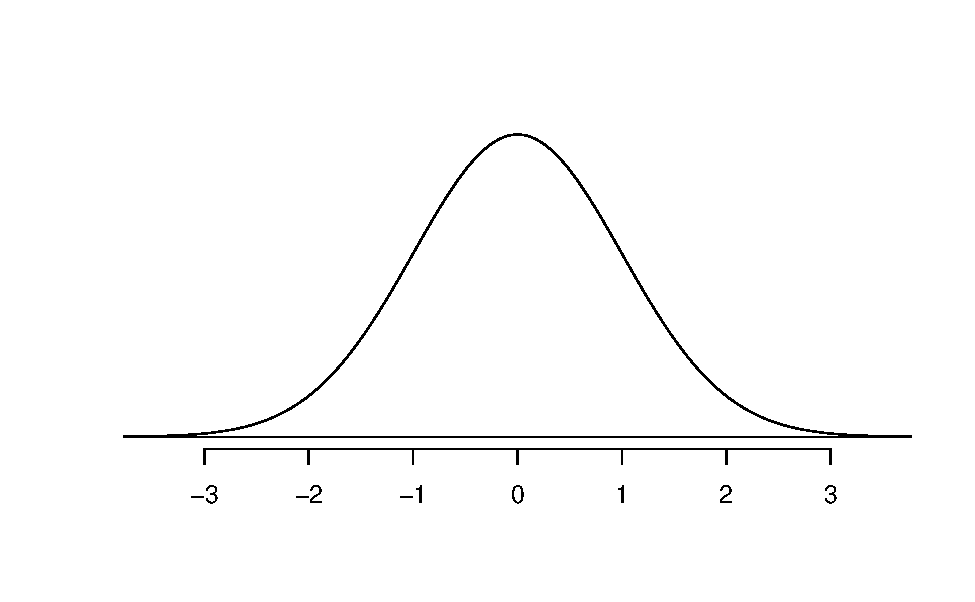
\includegraphics[width=0.5\linewidth]{07-A09-inference-1cat_test-theory_files/figure-latex/simpleNormalcurve-1} 

}

\caption{A standard normal curve.}\label{fig:simpleNormalcurve}
\end{figure}

\newpage

The standardized statistic measures the \emph{number of standard errors the sample statistic is from the null value}.

\begin{enumerate}
\def\labelenumi{\arabic{enumi}.}
\setcounter{enumi}{9}
\tightlist
\item
  Interpret the standardized sample proportion from question 8 in context of the problem.
\end{enumerate}

\vspace{.8in}

We will use the \texttt{pnorm()} function in R to find the p-value. Use the provided R script file and enter the value of the standardized statistic calculated in question 8 at \texttt{xx} in line 7; highlight and run lines 7--9. Notice that in line 9 it says \texttt{lower.tail\ =\ FALSE}. R will calculate the p-value \emph{greater} than the value of the standardized statistic.

Notes:

\begin{itemize}
\tightlist
\item
  Use \texttt{lower.tail\ =\ TRUE} when doing a left-sided test.
\item
  Use \texttt{lower.tail\ =\ FALSE} when doing a right-sided test.
\item
  To find a two-sided p-value, use a left-sided test for negative Z or a right-sided test for positive Z, then multiply the value found by 2 to get the p-value.
\end{itemize}

\begin{Shaded}
\begin{Highlighting}[]
\FunctionTok{pnorm}\NormalTok{(xx, }\CommentTok{\# Enter value of standardized statistic}
      \AttributeTok{m=}\DecValTok{0}\NormalTok{, }\AttributeTok{s=}\DecValTok{1}\NormalTok{, }\CommentTok{\# Using the standard normal mean = 0, sd = 1}
      \AttributeTok{lower.tail=}\ConstantTok{FALSE}\NormalTok{) }\CommentTok{\# Gives a p{-}value greater than the standardized statistic}
\end{Highlighting}
\end{Shaded}

\begin{enumerate}
\def\labelenumi{\arabic{enumi}.}
\setcounter{enumi}{10}
\item
  Report the p-value obtained from the R output.
  \vspace{0.3in}
\item
  Write a conclusion based on the value of the p-value.
  \newpage
\end{enumerate}

\hypertarget{impacts-on-the-p-value}{%
\subsection*{Impacts on the P-value}\label{impacts-on-the-p-value}}
\addcontentsline{toc}{subsection}{Impacts on the P-value}

Suppose that we want to show that the true proportion of male boxers \textbf{differs} from that in the general population.

\begin{enumerate}
\def\labelenumi{\arabic{enumi}.}
\setcounter{enumi}{12}
\tightlist
\item
  Write out the alternative hypothesis in notation for this new research question.
\end{enumerate}

\vspace{0.5in}

\begin{enumerate}
\def\labelenumi{\arabic{enumi}.}
\setcounter{enumi}{13}
\tightlist
\item
  How would this impact the p-value?
\end{enumerate}

\vspace{0.2in}

\begin{enumerate}
\def\labelenumi{\arabic{enumi}.}
\setcounter{enumi}{14}
\tightlist
\item
  How much evidence would this p-value provide against the null hypothesis?
\end{enumerate}

\vspace{0.3in}

\begin{enumerate}
\def\labelenumi{\arabic{enumi}.}
\setcounter{enumi}{15}
\tightlist
\item
  Suppose instead of 500 male boxers the researchers only took a sample of 300 male boxers and found the same proportion (\(\hat{p}=0.182\)) of male boxers that are left-handed. Since we are still assuming the same null value, 0.1, the standard error would be calculated as below:
\end{enumerate}

\[SE_0(\hat{p})=\sqrt{\frac{0.1(1-0.1)}{300}} = 0.017\].

Calculate the standardized statistic for this new sample.

\vspace{0.8in}

Use Rstudio to find the p-value for this new sample. Enter the value of the standardized statistic found in question 14 for xx in line 12. Highlight and run lines 12--14.

\begin{Shaded}
\begin{Highlighting}[]
\FunctionTok{pnorm}\NormalTok{(xx, }\CommentTok{\# Enter value of standardized statistic}
      \AttributeTok{m=}\DecValTok{0}\NormalTok{, }\AttributeTok{s=}\DecValTok{1}\NormalTok{, }\CommentTok{\# Using the standard normal mean = 0, sd = 1}
      \AttributeTok{lower.tail=}\ConstantTok{FALSE}\NormalTok{) }\CommentTok{\# Gives a p{-}value greater than the standardized statistic}
\end{Highlighting}
\end{Shaded}

\begin{enumerate}
\def\labelenumi{\arabic{enumi}.}
\setcounter{enumi}{16}
\tightlist
\item
  How does the decrease in sample size affect the p-value?
\end{enumerate}

\vspace{0.3in}

\begin{enumerate}
\def\labelenumi{\arabic{enumi}.}
\setcounter{enumi}{17}
\tightlist
\item
  Suppose another sample of 500 male boxers was taken and 68 were found to be left-handed. Since we are still assuming the same null value, 0.1, the standard error would be calculated as before:
\end{enumerate}

\[SE_0(\hat{p})=\sqrt{\frac{0.1(1-0.1)}{500}} = 0.013\].Calculate the standardized statistic for this new sample.

\vspace{0.8in}

Use Rstudio to find the p-value for this new sample.

\begin{Shaded}
\begin{Highlighting}[]
\FunctionTok{pnorm}\NormalTok{(xx, }\CommentTok{\# Enter value of standardized statistic}
      \AttributeTok{m=}\DecValTok{0}\NormalTok{, }\AttributeTok{s=}\DecValTok{1} \CommentTok{\# Using the standard normal mean = 0, sd = 1}
      \AttributeTok{lower.tail=}\ConstantTok{FALSE}\NormalTok{) }\CommentTok{\# Gives a p{-}value greater than the standardized statistic}
\end{Highlighting}
\end{Shaded}

\begin{enumerate}
\def\labelenumi{\arabic{enumi}.}
\setcounter{enumi}{18}
\tightlist
\item
  How does a statistic closer to the null value affect the p-value?
\end{enumerate}

\vspace{0.3in}

\begin{enumerate}
\def\labelenumi{\arabic{enumi}.}
\setcounter{enumi}{19}
\tightlist
\item
  Summarize how each of the following affected the p-value:
\end{enumerate}

\begin{enumerate}
\def\labelenumi{\alph{enumi})}
\tightlist
\item
  Switching to a two-sided test.
\end{enumerate}

\vspace{0.4in}

\begin{enumerate}
\def\labelenumi{\alph{enumi})}
\setcounter{enumi}{1}
\tightlist
\item
  Using a smaller sample size.
\end{enumerate}

\vspace{0.4in}

\begin{enumerate}
\def\labelenumi{\alph{enumi})}
\setcounter{enumi}{2}
\tightlist
\item
  Using a sample statistic closer to the null value.
\end{enumerate}

\vspace{0.4in}

\hypertarget{take-home-messages-11}{%
\subsection{Take-home messages}\label{take-home-messages-11}}

\begin{enumerate}
\def\labelenumi{\arabic{enumi}.}
\item
  Both simulation and theory-based methods can be used to find a p-value for a hypothesis test. In order to use theory-based methods we need to check that both the independence and the success-failure conditions are met.
\item
  The standardized statistic measures how many standard errors the statistic is from the null value. The larger the standardized statistic the more evidence there is against the null hypothesis.
\item
  The p-value for a two-sided test is approximately two times the value for a one-sided test. A two-sided test provides less evidence against the null hypothesis.
\item
  The larger the sample size, the smaller the sample to sample variability. This will result in a larger standardized statistic and more evidence against the null hypothesis.
\item
  The farther the statistic is from the null value, the larger the standardized statistic. This will result in a smaller p-value and more evidence against the null hypothesis.
\end{enumerate}

\newpage

\hypertarget{additional-notes-10}{%
\subsection{Additional notes}\label{additional-notes-10}}

Use this space to summarize your thoughts and take additional notes on today's activity and material covered.

\newpage

\hypertarget{activity-7b-handedness-of-male-boxers-theory-ci}{%
\section{Activity 7B: Handedness of Male Boxers --- Theory CI}\label{activity-7b-handedness-of-male-boxers-theory-ci}}

\setstretch{1}

\hypertarget{learning-objectives}{%
\subsection{Learning objectives}\label{learning-objectives}}

\begin{itemize}
\item
  Calculate a theory-based confidence interval for a single proportion.
\item
  Check the appropriate conditions to find a theory-based confidence interval.
\item
  Interpret a confidence interval for a single proportion.
\item
  Use the normal distribution to find the multiplier needed for a confidence interval
\end{itemize}

\hypertarget{terminology-review-11}{%
\subsection{Terminology review}\label{terminology-review-11}}

In this activity, we will introduce theory-based confidence intervals for a single proportion. Some terms covered in this activity are:

\begin{itemize}
\item
  Parameter of interest
\item
  Multiplier
\item
  Normal distribution
\end{itemize}

To review these concepts, see Chapters 11 \& 14 in your textbook.

\hypertarget{handedness-of-male-boxers-1}{%
\subsection{Handedness of Male Boxers}\label{handedness-of-male-boxers-1}}

Last class we found very strong evidence that the true proportion of male boxers that are left-handed is greater than 0.1. In this activity we will use the same data set to find the theory-based 95\% confidence interval.

Remember from the last activity: Left-handedness is a trait that is found in about 10\% of the general population. Past studies have shown that left-handed men are over-represented among professional boxers. The fighting claim states that left-handed men have an advantage in competition. In this random sample of 500 male professional boxers, we want to see if there is an over-prevalence of left-handed fighters. In the sample of 500 male boxers, 81 were left-handed.

Recall that to use theory-based methods we must check the conditions to approximate the sampling distribution with the normal distribution. From the previous activity, we saw that independence was satisfied as the researchers took a random sample and that the sample had more than 10 successes and 10 failures.

\newpage

\hypertarget{theory-based-confidence-interval}{%
\subsubsection*{Theory-based confidence interval}\label{theory-based-confidence-interval}}
\addcontentsline{toc}{subsubsection}{Theory-based confidence interval}

To calculate a theory-based 95\% confidence interval for \(\pi\), we will first find the \textbf{standard error} of \(\hat{p}\) by plugging in the value of \(\hat{p}\) for \(\pi\) in \(SD(\hat{p})\):

\[SE(\hat{p}) = \sqrt{\frac{\hat{p}(1-\hat{p})}{n}}.\]
Note that we do not include a ``0'' subscript, since we are not assuming a null hypothesis.

\begin{enumerate}
\def\labelenumi{\arabic{enumi}.}
\tightlist
\item
  Calculate the standard error of the sample proportion to find a 95\% confidence interval.
\end{enumerate}

\vspace{0.5in}

To find the confidence interval, we will add and subtract the \textbf{margin of error} to the point estimate:

\[\text{point estimate}\pm\text{margin of error}\]
\[\hat{p}\pm z^* SE(\hat{p})\]
\[ME = z^* SE(\hat{p})\]

The \(z^*\) multiplier is the percentile of a standard normal distribution that corresponds to our confidence level. If our confidence level is 95\%, we find the Z values that encompass the middle 95\% of the standard normal distribution. If 95\% of the standard normal distribution should be in the middle, that leaves 5\% in the tails, or 2.5\% in each tail.

\begin{enumerate}
\def\labelenumi{\arabic{enumi}.}
\setcounter{enumi}{1}
\tightlist
\item
  Fill in the normal distribution shown in figure 7.2 to show how R found the \(z^*\) multiplier.
\end{enumerate}

\begin{figure}

{\centering 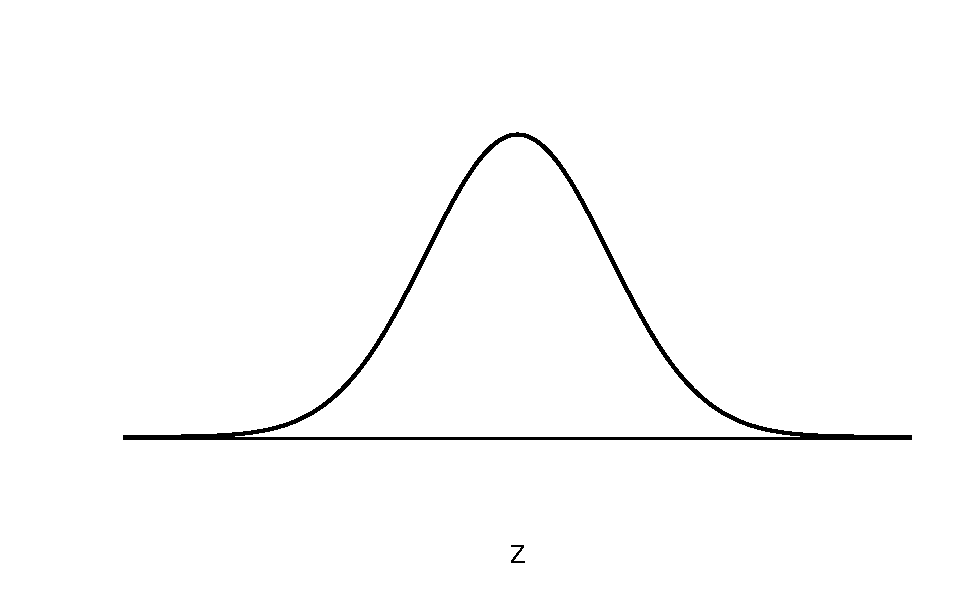
\includegraphics[width=0.5\linewidth]{07-A10-inference-1cat_CI-theory_files/figure-latex/simpleNormaldist-1} 

}

\caption{A standard normal curve.}\label{fig:simpleNormaldist}
\end{figure}

The \texttt{qnorm()} function in R will tell us the \(z^*\) value for the desired percentile (in this case, 95\% + 2.5\% = 97.5\% percentile). Enter the value of 0.975 for xx in the provided R script file. This will give the value of the multiplier for a 95\% confidence interval.

\begin{Shaded}
\begin{Highlighting}[]
\FunctionTok{qnorm}\NormalTok{(xx) }\CommentTok{\# Multiplier for 95\% confidence interval}
\end{Highlighting}
\end{Shaded}

\begin{enumerate}
\def\labelenumi{\arabic{enumi}.}
\setcounter{enumi}{2}
\item
  Report the value of the multiplier needed to calculate the 95\% confidence interval for the true proportion of male boxers that are left-handed?
  \vspace{0.3in}
\item
  Calculate the margin of error for the 95\% confidence interval.
  \vspace{1in}
\item
  Calculate the 95\% confidence interval for the parameter of interest.
  \vspace{0.5in}
\item
  Interpret the 95\% confidence interval in the context of the problem.
  \vspace{1in}
\item
  Is the null value, 0.1, contained in the 95\% confidence interval? Explain, based on the p-value from the last activity, why you expected this to be true.
  \vspace{0.5in}
\end{enumerate}

\hypertarget{simulation-methods}{%
\subsubsection*{Simulation Methods}\label{simulation-methods}}
\addcontentsline{toc}{subsubsection}{Simulation Methods}

In activity 7A, we found that the success-failure condition was met to use theory-based methods. Here we will use simulation methods to find a 95\% confidence interval for the parameter of interest.

Use the \texttt{one\_proportion\_bootstrap\_CI()} function in R to simulate the bootstrap distribution of sample proportions and calculate a confidence interval. Using the provided R script file, fill in the values/words for each \texttt{xx} in the one proportion bootstrap confidence interval (CI) code to create a bootstrap distribution with 1000 simulations. Make sure to run the library(catstats) function before running the one\_proportion\_bootstrap\_CI function.

\begin{Shaded}
\begin{Highlighting}[]
\FunctionTok{one\_proportion\_bootstrap\_CI}\NormalTok{(}\AttributeTok{sample\_size =}\NormalTok{ xx, }\CommentTok{\# Sample size}
                    \AttributeTok{number\_successes =}\NormalTok{ xx, }\CommentTok{\# Observed number of successes}
                    \AttributeTok{number\_repetitions =} \DecValTok{1000}\NormalTok{, }\CommentTok{\# Number of bootstrap samples to use}
                    \AttributeTok{confidence\_level =} \FloatTok{0.95}\NormalTok{) }\CommentTok{\# Confidence level as a decimal}
\end{Highlighting}
\end{Shaded}

\begin{enumerate}
\def\labelenumi{\arabic{enumi}.}
\setcounter{enumi}{7}
\tightlist
\item
  Report the simulation 95\% confidence interval. Is this confidence interval similar to the confidence interval calculated in question 5? Explain why this makes sense.
\end{enumerate}

\vspace{0.8in}

\hypertarget{what-does-confidence-mean}{%
\subsection*{\texorpdfstring{What does \emph{confidence} mean?}{What does confidence mean?}}\label{what-does-confidence-mean}}
\addcontentsline{toc}{subsection}{What does \emph{confidence} mean?}

In the interpretation of a 95\% confidence interval, we say that we are 95\% confident that the parameter is within the confidence interval. Why are we able to make that claim? What does it mean to say ``we are 95\% confident''?

For this part of the activity we will assume that the the true proportion of male boxers that are left-handed is 0.1. \emph{Note: we are making assumptions about the population here. This is not based on our calculated data, but we will use this applet to better understand what happens when we take many, many samples from this believed population.}

\begin{enumerate}
\def\labelenumi{\arabic{enumi}.}
\setcounter{enumi}{8}
\item
  Go to this website, \url{http://www.rossmanchance.com/ISIapplets.html} and choose `Simulating Confidence Intervals'. In the input on the left-hand side of the screen enter 0.1 for \(\pi\) (the true value), 500 for \(n\), and 100 for `Number of intervals'. Click `sample'.
  \vspace{1mm}

  \begin{enumerate}
  \def\labelenumii{\alph{enumii}.}
  \item
    In the graph on the bottom right, click on a green dot. Write down the confidence interval for this sample given on the graph on the left. Does this confidence interval contain the true value of 0.1?
    \vspace{0.5in}
  \item
    Now click on a red dot. Write down the confidence interval for this sample. Does this confidence interval contain the true value of 0.1?
    \vspace{0.5in}
  \item
    How many intervals out of 100 contain \(\pi\), the true value of 0.1? \emph{Hint}: This is given to the left of the graph of green and red intervals.
    \vspace{0.5in}
  \end{enumerate}
\item
  Click on `sample' nine more times. Write down the `Running Total' for the proportion of intervals that contain \(\pi\).
\end{enumerate}

\vspace{0.5in}

\begin{enumerate}
\def\labelenumi{\arabic{enumi}.}
\setcounter{enumi}{10}
\tightlist
\item
  \textbf{Interpret the level of confidence. \emph{Hint}: What proportion of samples would we expect to give a confidence interval that contains the parameter of interest?}
\end{enumerate}

\vspace{0.8in}

\hypertarget{take-home-messages-12}{%
\subsection{Take-home messages}\label{take-home-messages-12}}

\begin{enumerate}
\def\labelenumi{\arabic{enumi}.}
\item
  In theory-based methods, we add and subtract a margin of error to the sample statistic. The margin of error is calculated using a multiplier that corresponds to the level of confidence times the variability (standard error) of the statistic.
\item
  The confidence interval calculated using theory-based methods should be similar to the confidence interval found using simulation methods provided the success-failure condition is met.
\end{enumerate}

\begin{enumerate}
\def\labelenumi{\arabic{enumi}.}
\setcounter{enumi}{2}
\tightlist
\item
  If repeat samples of the same size are selected from the population, approximately 95\% of samples will create a 95\% confidence interval that contains the parameter of interest.
\end{enumerate}

\hypertarget{additional-notes-11}{%
\subsection{Additional notes}\label{additional-notes-11}}

Use this space to summarize your thoughts and take additional notes on today's activity and material covered.

\newpage

\hypertarget{week-7-lab-errors-and-power}{%
\section{Week 7 Lab: Errors and Power}\label{week-7-lab-errors-and-power}}

\setstretch{1}

\hypertarget{learning-outcomes-13}{%
\subsection{Learning outcomes}\label{learning-outcomes-13}}

\begin{itemize}
\item
  Explain type 1 and type 2 errors in the context of a study.
\item
  Explain the power of a test in the context of a study.
\item
  Understand how changes in sample size, significance level, and the difference between the null value and the parameter value impact the power of a test.
\item
  Understand how significance level impacts the probability of a type 1 error.
\item
  Understand the relationship between the probability of a type 2 error and power.
\item
  Be able to distinguish between practical importance and statistical significance.
\end{itemize}

\hypertarget{terminology-review-12}{%
\subsection{Terminology review}\label{terminology-review-12}}

In this activity, we will examine the possible errors that can be made based on the decision in a hypothesis test as well as factors influencing the power of the test. Some terms covered in this activity are:

\begin{itemize}
\item
  Significance level
\item
  Type 1 error
\item
  Type 2 error
\item
  Power
\end{itemize}

To review these concepts, see Chapter 12 in the textbook.

\hypertarget{acl-recovery}{%
\subsection{ACL recovery}\label{acl-recovery}}

It is widely reported that the median recovery time for athletes who undergo surgery to repair a torn anterior cruciate ligament (ACL) is 8 months, indicating that 50\% of athletes return to their sport within 8 months after an ACL surgery. Suppose a local physical therapy company hopes to advertise that their rehabilitation program can increase this percentage.

\begin{enumerate}
\def\labelenumi{\arabic{enumi}.}
\item
  Write the parameter of interest (\(\pi\)) in words, in the context of this problem.
  \vspace{0.5in}
\item
  \textbf{Use proper notation to write the null and alternative hypothesis the company would need to test in order to check their advertisement claim.}
  \vspace{0.5in}
\end{enumerate}

After determining hypotheses and prior to collecting data, researchers should set a \textbf{significance level} for a hypothesis test. The significance level, represented by \(\alpha\) and most commonly 0.01, 0.05, or 0.10, is a cut-off for determining whether a p-value is small or not. The \emph{smaller} the p-value, the \emph{stronger} the evidence against the null hypothesis, so a p-value that is smaller than or equal to the significance level is strong enough evidence to \emph{reject the null hypothesis}. Similarly, the \emph{larger} the p-value, the \emph{weaker} the evidence against the null hypothesis, so a p-value that is larger than the significance level does not provide enough evidence against the null hypothesis and the researcher would \emph{fail to reject the null hypothesis}. Rejecting the null hypothesis or failing to reject the null hypothesis are the two \textbf{decisions} that can be made based on the data collected.

As you have already learned in this course, sample size of a study is extremely important. Often times, researchers will conduct what is called a power analysis to determine the appropriate sample size based on the goals of their research, including a desired \textbf{power} of their test. Power is the probability of correctly rejecting the null hypothesis, or the probability of the data providing strong evidence against the null hypothesis \emph{when the null hypothesis is false}.

The remainder of this lab will be spent investigating how different factors influence the power of a test, after which you will complete a power analysis for this physical therapy company.

\begin{itemize}
\item
  Navigate to \url{https://istats.shinyapps.io/power/}. \emph{Please note that this applet uses \(p_0\) to represent the null value rather than \(\pi_0\).}
\item
  Use the scale under ``Null Hypothesis value \(p_0\)'' to change the value to your null value from question 2.
\item
  Change the ``Alternative Hypothesis'' to the direction you wrote in question 2.
\item
  Leave all boxes un-checked. Do not change the scales under ``True value of \(p_0\)'', ``Sample size n'', or ``Type I Error \(\alpha\)''
\end{itemize}

The red distribution you see is the scaled-Normal distribution representing the null distribution for this hypothesis test, if the sample size was 50 and the significance level was 0.05. This means the red distribution is showing the probability of each possible sample proportion of athletes who returned to their sport within 8 months (\(\hat{p}\)) if we assume the null hypothesis is true.

\begin{enumerate}
\def\labelenumi{\arabic{enumi}.}
\setcounter{enumi}{2}
\item
  Based off this distribution and your alternative hypothesis, give one possible sample proportion which you think would lead to rejecting the null hypothesis. Explain how you decided on your value.
  \vspace{0.25in}
\item
  Check the box for ``Show Critical Value(s) and Rejection Region(s)''. You will now see a vertical line on the plot indicating the \emph{minimum} sample proportion which would lead to reject the null hypothesis. What is this value?\\
  \vspace{0.25in}
\item
  Notice that there are some sample proportions under the red line (when the null hypothesis is true) which would lead us to reject the null hypothesis. Give the range of sample proportions which would lead to rejecting the null hypothesis when the null hypothesis is true? What is the statistical name for this mistake?
  \vspace{0.4in}
\end{enumerate}

Check the ``Type I Error'' box under \textbf{Display}. This should verify (or correct) your answer to question 5! The area shaded in red represents the probability of making a \textbf{type 1 error} in our hypothesis test. Recall that a type 1 error is when we reject the null hypothesis even though the null hypothesis is true. To reject the null hypothesis, the p-value, which was found assuming the null hypothesis is true, must be less than or equal to the significance level. Therefore the significance level is the maximum probability of rejecting the null hypothesis when the null hypothesis is true, so the significance level IS the probability of making a type 1 error in a hypothesis test!

\begin{enumerate}
\def\labelenumi{\arabic{enumi}.}
\setcounter{enumi}{5}
\tightlist
\item
  \textbf{Based on the current applet settings, What percent of the null distribution is shaded red (what is the probability of making a type 1 error)?}
  \vspace{0.25in}
\end{enumerate}

Let's say this physical therapist company believes their program can get 70\% of athletes back to their sport within 8 months of an ACL surgery. In the applet, set the scale under ``True value of \(p\)'' to 0.7.

\begin{enumerate}
\def\labelenumi{\arabic{enumi}.}
\setcounter{enumi}{6}
\tightlist
\item
  Where is the blue distribution centered?
  \vspace{0.25in}
\end{enumerate}

The blue distribution that appears represents what the company believes, that 0.7 (not 0.5) is the true proportion of its clients who return to their sport within 8 months of ACL surgery. This blue distribution represents the idea that the \textbf{null hypothesis is false}.

\begin{enumerate}
\def\labelenumi{\arabic{enumi}.}
\setcounter{enumi}{7}
\tightlist
\item
  Consider the definition of power provided earlier in this lab. Do you believe the power of the test will be an area within the blue distribution or red distribution? How do you know? What about the probability of making a type 2 error?
  \vspace{1in}
\end{enumerate}

\begin{itemize}
\tightlist
\item
  Check the ``Type II Error'' and ``Power'' boxes under \textbf{Display}. This should verify (or correct) your answers to question 8! The area shaded in blue represents the probability of making a \textbf{type 2 error} in our hypothesis test (failing to reject the null hypothesis even though the null hypothesis is false). The area shaded in green represents the power of the test. Notice that the type 1 and type 2 errors rates and the power of the test are provided above the distribution.
\end{itemize}

\begin{enumerate}
\def\labelenumi{\arabic{enumi}.}
\setcounter{enumi}{8}
\tightlist
\item
  \textbf{Complete the following equation: Power + Type 2 Error Rate = . Explain why that equation makes sense.} \emph{Hint: Consider what power and type 2 error are conditional on.}
  \vspace{0.8in}
\end{enumerate}

Now let's investigate how changes in different factors influence the power of a test.

\begin{enumerate}
\def\labelenumi{\arabic{enumi}.}
\setcounter{enumi}{9}
\item
  Using the same sample size and significance level, change the ``True value of \(p\)'' to see the effect on Power.
  \setlength\tabcolsep{0.5cm}

  \begin{longtable}{|l|c|c|c|c|c|}
  \hline
  \textbf{True value of $p$}& 0.60 & 0.65 & 0.70 & 0.75 & 0.80 \\ \hline
  \textbf{Power} & & & & &  \\ \hline
  \end{longtable}
\item
  What is changing about the simulated distributions pictured as you change the ``True value of \(p\)''?
  \vspace{0.5in}
\item
  \textbf{How does increasing the distance between the null and believed true probability of success affect the power of the test?}
  \vspace{0.5in}
\item
  Using the same significance level, set the ``True value of \(p\)'' to 0.7 and change the sample size to see the effect on Power.
\end{enumerate}

\setlength\tabcolsep{0.6cm}
\begin{longtable}{|l|c|c|c|c|c|}
\hline
\textbf{Sample Size}& 20 & 40 & 50 & 60 & 80 \\ \hline
\textbf{Power} & & & & &  \\ \hline
\end{longtable}

\begin{enumerate}
\def\labelenumi{\arabic{enumi}.}
\setcounter{enumi}{13}
\item
  What is changing about the simulated distributions pictured as you change the sample size?
  \vspace{0.5in}
\item
  \textbf{How does increasing the sample size affect the power of the test?}
  \vspace{0.5in}
\item
  Using the same ``True value of \(p\)'', set the sample size to 50 and change the ``Type I Error \(\alpha\)'' to see the effect on Power.
\end{enumerate}

\setlength\tabcolsep{0.5cm}
\begin{longtable}{|l|c|c|c|c|c|}
\hline
\textbf{Type I Error $\alpha$}& 0.01 & 0.03 & 0.05 & 0.10 & 0.15 \\ \hline
\textbf{Power} & & & & &  \\ \hline
\end{longtable}

\begin{enumerate}
\def\labelenumi{\arabic{enumi}.}
\setcounter{enumi}{16}
\item
  What is changing about the simulated distributions pictured as you change the significance level?
  \vspace{0.5in}
\item
  \textbf{How does increasing the significance level affect the power of the test?}
  \vspace{0.5in}
\item
  \textbf{Complete the power analysis for this physical therapy company. The company believes 70\% of their patients will return to their sport within 8 months of ACL surgery. They want to limit the probability of a type 1 error to 10\% and the probability of a type 2 error to 15\%. What is the minimum number of athletes the company will need to collect data from in order to meet these goals? Use the applet to answer this question, then download your image created and upload the file to Gradescope.}
  \vspace{0.25in}
\end{enumerate}

\newpage

\begin{enumerate}
\def\labelenumi{\arabic{enumi}.}
\setcounter{enumi}{19}
\tightlist
\item
  Based on the goals outlined in question 19, which mistake below is the company more concerned about? In other words, which error were the researchers trying to minimize. Explain your answer.
\end{enumerate}

\begin{itemize}
\item
  Not being able to advertise their ACL recovery program is better than average when their program really is better.
\item
  Advertising their ACL recovery program is better even though it is not.
\end{itemize}

\vspace{0.8in}

\newpage

\hypertarget{inference-for-two-categorical-variables-simulation-based-methods}{%
\chapter{Inference for Two Categorical Variables: Simulation-based Methods}\label{inference-for-two-categorical-variables-simulation-based-methods}}

\hypertarget{week-8-reading-guide-hypothesis-testing-for-a-difference-in-proportions}{%
\section{Week 8 Reading Guide: Hypothesis Testing for a Difference in Proportions}\label{week-8-reading-guide-hypothesis-testing-for-a-difference-in-proportions}}

\hypertarget{section-15.1-randomization-test-for-h_0-pi_1---pi_2-0-and-section-15.2-bootstrap-confidence-interval-for-pi_1---pi_2}{%
\subsection*{\texorpdfstring{Section 15.1 (Randomization test for \(H_0: \pi_1 - \pi_2 = 0\)) and Section 15.2 (Bootstrap confidence interval for \(\pi_1 - \pi_2\))}{Section 15.1 (Randomization test for H\_0: \textbackslash pi\_1 - \textbackslash pi\_2 = 0) and Section 15.2 (Bootstrap confidence interval for \textbackslash pi\_1 - \textbackslash pi\_2)}}\label{section-15.1-randomization-test-for-h_0-pi_1---pi_2-0-and-section-15.2-bootstrap-confidence-interval-for-pi_1---pi_2}}
\addcontentsline{toc}{subsection}{Section 15.1 (Randomization test for \(H_0: \pi_1 - \pi_2 = 0\)) and Section 15.2 (Bootstrap confidence interval for \(\pi_1 - \pi_2\))}

You may skip example 15.1.4, which discussed hypothesis testing for \textbf{relative risk}. We will discuss relative risk in Week 14.

\textbf{Videos}

\begin{itemize}
\tightlist
\item
  15.1
\item
  15.2
\end{itemize}

\setstretch{1.25}

\hypertarget{reminders-from-previous-sections-7}{%
\subsubsection*{Reminders from previous sections}\label{reminders-from-previous-sections-7}}
\addcontentsline{toc}{subsubsection}{Reminders from previous sections}

\(n\) = sample size

\(\hat{p}\) = sample proportion

\(\pi\) = population proportion

General steps of a hypothesis test:

\begin{enumerate}
\def\labelenumi{\arabic{enumi}.}
\item
  Frame the research question in terms of hypotheses.
\item
  Collect and summarize data using a test statistic.
\item
  Assume the null hypothesis is true, and simulate or mathematically model a null distribution for the test statistic.
\item
  Compare the observed test (standardized) statistic to the null distribution to calculate a p-value.
\item
  Make a conclusion based on the p-value and write the conclusion in context.
\end{enumerate}

Parameter: a value summarizing a variable(s) for a population.

Statistic: a value summarizing a variable(s) for a sample.

Sampling distribution: plot of statistics from 1000s of samples of the same size taken from the same population.

Standard deviation of a statistic: the variability of statistics from 1000s of samples; how far, on average, each statistic is from the true value of the parameter.

Standard error of a statistic: estimated standard deviation of a statistic.

Hypothesis test: a process to determine how strong the evidence of an effect is.

\rgi Also called a `significance test'.

Simulation-based method: Simulate lots of samples of size \(n\) under assumption of the null hypothesis, then find the proportion of the simulations that are at least as extreme as the observed sample statistic.

Null hypothesis (\(H_0\)): the skeptical perspective; no difference; no change; no effect; random chance; what the researcher hopes to prove is \textbf{wrong}.

Alternative hypothesis (\(H_A\)): the new perspective; a difference/increase/decrease; an effect; not random chance; what the researcher hopes to prove is \textbf{correct}.

Null value: the value of the parameter when we assume the null hypothesis is true (labeled as \(parameter_0\)).

Null distribution: the simulated or modeled distribution of statistics (sampling distribution) we would expect to occur if the null hypothesis is true.

P-value: probability of seeing the observed sample data, or something more extreme, assuming the null hypothesis is true.

\(\implies\) Lower the p-value the stronger the evidence AGAINST the null hypothesis and FOR the alternative hypothesis.

Decision: a determination of whether to `reject' or `fail to reject' a null hypothesis based on a p-value and a pre-set level of significance.

Significance level (\(\alpha\)): a threshold used to determine if a p-value provides enough evidence to reject the null hypothesis or not.

\rgi Common levels of \(\alpha\) include 0.01, 0.05, and 0.10.

Statistically significant: results are considered statistically significant if the p-value is below the significance level.

Confidence interval: a process to determine how large an effect is; a range of plausible values for the parameter. Also called `estimation'.

Margin of error: the value that is added to and subtracted from the sample statistic to create a confidence interval; half the width of a confidence interval.

Bootstrapping: the process of drawing with replacement \(n\) times from the original sample.

Bootstrapped resample: a random sample of size \(n\) from the original sample, selected with replacement.

Bootstrapped statistic: the statistic recorded from the bootstrapped resample.

Confidence level: how confident we are that the confidence interval will capture the parameter.

\hypertarget{vocabulary-16}{%
\subsubsection*{Vocabulary}\label{vocabulary-16}}
\addcontentsline{toc}{subsubsection}{Vocabulary}

Randomization test:
\rgs

\hypertarget{notes-20}{%
\subsubsection*{Notes}\label{notes-20}}
\addcontentsline{toc}{subsubsection}{Notes}

In a randomization test involving two categorical variables,

\rgi how many cards will you need and how will the cards be labeled?
\rgs

\rgi Why, in the randomization test, are the cards all shuffled together and randomly dealt into two new groups?
\rgs

\rgi After shuffling, how many cards are dealt into each pile?
\rgs

To create a single bootstrap resample for two categorical variables,

\rgi how many cards will you need and how will the cards be labeled?
\rgs

\rgi What is done with the cards once they are labeled?
\rgs

Interpretations of confidence level must include:
\rgs
\rgs

How do you determine if the results of a hypothesis test agree with a confidence interval?
\rgs
\rgs

How are the confidence level and the significance level related (for a two-sided test)?
\rgs

\hypertarget{notation}{%
\subsubsection*{Notation}\label{notation}}
\addcontentsline{toc}{subsubsection}{Notation}

Sample size of group 1:
\rgs

Sample size of group 2:
\rgs

Sample proportion of group 1:
\rgs

Sample proportion of group 2:
\rgs

Population proportion of group 1:
\rgs

Population proportion of group 2:
\rgs

\hypertarget{example-gender-discrimination}{%
\subsubsection*{Example: Gender discrimination}\label{example-gender-discrimination}}
\addcontentsline{toc}{subsubsection}{Example: Gender discrimination}

\begin{enumerate}
\def\labelenumi{\arabic{enumi}.}
\item
  What is the research question?
  \rgs
\item
  What are the observational units?
  \rgs
\item
  What type of study design was used? Justify your answer.
  \rgs
\item
  What is the appropriate scope of inference for these data?
  \rgs
\item
  What is the sample statistic presented in this example? What notation would be used to represent this value?
  \rgs
\item
  What is the parameter representing in the context of this problem? What notation would be used to represent this parameter?
  \rgs
  \rgs
\item
  Write the null and the alternative hypotheses in words.
  \rgs
  \rgs
\item
  Write the null and the alternative hypotheses in notation.
  \rgs
\item
  How could we use cards to simulate \textbf{one} sample \emph{which assumes the null hypothesis is true}? How many blue cards --- to represent what? How many red cards --- to represent what? What would we do with the cards? What would you record once you have a simulated sample?
  \rgs
  \rgs
  \rgs
\item
  How can we calculate a p-value from the simulated null distribution for this example?
  \rgs
  \rgs
\item
  What was the p-value of the test?
  \rgs
\item
  At the 5\% significance level, what decision would you make?
  \rgs
\item
  What conclusion should the researcher make?
  \rgs
  \rgs
\item
  Are the results in this example statistically significant? Justify your answer.
  \rgs
\end{enumerate}

\hypertarget{example-opportunity-cost}{%
\subsubsection*{Example: Opportunity cost}\label{example-opportunity-cost}}
\addcontentsline{toc}{subsubsection}{Example: Opportunity cost}

\begin{enumerate}
\def\labelenumi{\arabic{enumi}.}
\item
  What is the research question?
  \rgs
\item
  What are the observational units?
  \rgs
\item
  What type of study design was used? Justify your answer.
  \rgs
\item
  What is the appropriate scope of inference for these data?
  \rgs
\item
  What is the sample statistic presented in this example? What notation would be used to represent this value?
  \rgs
\item
  What is the parameter representing in the context of this problem? What notation would be used to represent this parameter?
  \rgs
  \rgs
\item
  Write the null and the alternative hypotheses in words.
  \rgs
  \rgs
\item
  Write the null and the alternative hypotheses in notation.
  \rgs
\item
  How could we use cards to simulate \textbf{one} sample \emph{which assumes the null hypothesis is true}? How many blue cards --- to represent what? How many red cards --- to represent what? What would we do with the cards? What would you record once you have a simulated sample?
  \rgs
  \rgs
  \rgs
\item
  How can we calculate a p-value from the simulated null distribution for this example?
  \rgs
  \rgs
\item
  What was the p-value of the test?
  \rgs
\item
  Interpret the p-value in the context of the problem.
  \rgs
  \rgs
\item
  At the 5\% significance level, what decision would you make?
  \rgs
\item
  What conclusion should the researcher make?
  \rgs
\item
  Are the results in this example statistically significant? Justify your answer.
  \rgs
\end{enumerate}

\hypertarget{example-cpr-and-blood-thinners}{%
\subsubsection*{Example: CPR and blood thinners}\label{example-cpr-and-blood-thinners}}
\addcontentsline{toc}{subsubsection}{Example: CPR and blood thinners}

\begin{enumerate}
\def\labelenumi{\arabic{enumi}.}
\item
  What is the research question?
  \rgs
\item
  What are the observational units?
  \rgs
\item
  What type of study design was used? Justify your answer.
  \rgs
\item
  What is the appropriate scope of inference for these data?
  \rgs
\item
  What is the sample difference in proportions presented in this example? What notation would be used to represent this value?
  \rgs
\item
  What is the parameter (using a difference in proportions) representing in the context of this problem? What notation would be used to represent this parameter?
  \rgs
  \rgs
\item
  Write the null and the alternative hypotheses in words.
  \rgs
  \rgs
\item
  Write the null and the alternative hypotheses in notation.
  \rgs
\item
  How could we use cards to simulate \textbf{one} sample \emph{which assumes the null hypothesis is true}? How many blue cards --- to represent what? How many red cards --- to represent what? What would we do with the cards? What would you record once you have a simulated sample?
  \rgs
  \rgs
  \rgs
\item
  How can we calculate a p-value from the simulated null distribution for this example?
  \rgs
  \rgs
\item
  What was the p-value of the test?
  \rgs
\item
  Interpret the p-value in the context of the problem.
  \rgs
  \rgs
\item
  At the 5\% significance level, what decision would you make?
  \rgs
\item
  What conclusion should the researcher make?
  \rgs
  \rgs
\item
  Are the results in this example statistically significant? Justify your answer.
  \rgs
\item
  How could we use cards to simulate \textbf{one} bootstrap resample? How many blue cards --- to represent what? How many red cards --- to represent what? What would we do with the cards? What would you record once you have a simulated sample?
  \rgs
  \rgs
  \rgs
\item
  How can we calculate a 90\% confidence interval from the bootstrap distribution for this example?
  \rgs
\item
  What was the 90\% confidence interval?
  \rgs
\item
  Interpret the confidence \emph{interval} ((-0.03, 0.28)) in the context of the problem.
  \rgs
  \rgs
\item
  Interpret the confidence \emph{level} (90\%) in the context of the problem.
  \rgs
  \rgs
\item
  Does the conclusion of the hypothesis test match the confidence interval?
  \rgs
\end{enumerate}

\newpage

\hypertarget{activity-8a-the-good-samaritan-simulation-based-hypothesis-test}{%
\section{Activity 8A: The Good Samaritan --- Simulation-based Hypothesis Test}\label{activity-8a-the-good-samaritan-simulation-based-hypothesis-test}}

\setstretch{1}

\hypertarget{learning-outcomes-14}{%
\subsection{Learning outcomes}\label{learning-outcomes-14}}

\begin{itemize}
\item
  Given a research question involving two categorical variables, construct the null and alternative hypotheses
  in words and using appropriate statistical symbols.
\item
  Describe and perform a simulation-based hypothesis test for a difference in proportions.
\item
  Interpret and evaluate a p-value for a simulation-based hypothesis test for a difference in proportions.
\end{itemize}

\hypertarget{terminology-review-13}{%
\subsection{Terminology review}\label{terminology-review-13}}

In today's activity, we will use simulation-based methods to analyze two categorical variables. Some terms covered in this activity are:

\begin{itemize}
\item
  Conditional proportion
\item
  Null hypothesis
\item
  Alternative hypothesis
\end{itemize}

To review these concepts, see Chapter 15 in your textbook.

\hypertarget{the-good-samaritan}{%
\subsection{The Good Samaritan}\label{the-good-samaritan}}

Researchers at the Princeton University wanted to investigate influences on behavior (Darley and Batson 1973). The researchers randomly selected 67 students from the Princeton Theological Seminary to participate in a study. Only 47 students chose to participate in the study, and the data below includes 40 of those students (7 students were removed from the study for various reasons). As all participants were theology majors planning a career as a preacher, the expectation was that all would have a similar disposition when it comes to helping behavior. Each student was then shown a 5-minute presentation on the Good Samaritan, a parable in the Bible which emphasizes the importance of helping others. After the presentation, the students were told they needed to give a talk on the Good Samaritan parable at a building across campus. Half the students were told they were late for the presentation; the other half told they could take their time getting across campus (the condition was randomly assigned). On the way between buildings, an actor pretending to be a homeless person in distress asked the student for help. The researchers recorded whether the student helped the actor or not. The results of the study are shown in the table below. Do these data provide evidence that those in a hurry will be less likely to help people in need in this situation? Use the order of subtraction hurry -- no hurry.

\begin{longtable}[]{@{}llll@{}}
\toprule()
& Hurry Condition & No Hurry Condition & Total \\
\midrule()
\endhead
Helped Actor & 2 & 11 & 13 \\
Did Not Help Actor & 18 & 9 & 27 \\
Total & 20 & 20 & 40 \\
\bottomrule()
\end{longtable}

\newpage

These counts can be found in R by using the \texttt{count()} function:

\begin{Shaded}
\begin{Highlighting}[]
\CommentTok{\# Read data set in}
\NormalTok{good }\OtherTok{\textless{}{-}} \FunctionTok{read.csv}\NormalTok{(}\StringTok{"https://math.montana.edu/courses/s216/data/goodsam.csv"}\NormalTok{) }
\NormalTok{good }\SpecialCharTok{\%\textgreater{}\%} \FunctionTok{group\_by}\NormalTok{(Condition) }\SpecialCharTok{\%\textgreater{}\%} \FunctionTok{count}\NormalTok{(Behavior)}
\end{Highlighting}
\end{Shaded}

\begin{verbatim}
#> # A tibble: 4 x 3
#> # Groups:   Condition [2]
#>   Condition Behavior     n
#>   <chr>     <chr>    <int>
#> 1 Hurry     Help         2
#> 2 Hurry     No help     18
#> 3 No hurry  Help        11
#> 4 No hurry  No help      9
\end{verbatim}

\hypertarget{vocabulary-review-1}{%
\subsubsection*{Vocabulary review}\label{vocabulary-review-1}}
\addcontentsline{toc}{subsubsection}{Vocabulary review}

\begin{enumerate}
\def\labelenumi{\arabic{enumi}.}
\tightlist
\item
  What is the name of the explanatory variable as it is written in the R output? What are its categories?
\end{enumerate}

\vspace{0.2in}

\begin{enumerate}
\def\labelenumi{\arabic{enumi}.}
\setcounter{enumi}{1}
\tightlist
\item
  What is the response variable in the R output? What are its categories?
\end{enumerate}

\vspace{0.2in}

\setstretch{1.5}

\begin{enumerate}
\def\labelenumi{\arabic{enumi}.}
\setcounter{enumi}{2}
\tightlist
\item
  Fill in the blanks with one answer from each set of parentheses: This is an\\
  \_\_\_\_\_\_\_\_\_\_\_\_\_\_\_\_ (experiment/observational study) because\\
  \_\_\_\_\_\_\_\_\_\_\_\_\_\_ (hurry or no hurry/help or no help) \_\_\_\_\_\_\_ (was/was not)\\
  randomly \_\_\_\_\_\_\_\_\_\_\_\_ (assigned/selected).
\end{enumerate}

\vspace{0.1in}

\begin{enumerate}
\def\labelenumi{\arabic{enumi}.}
\setcounter{enumi}{3}
\tightlist
\item
  Put an X in the box that represents the appropriate scope of inference for this study.
\end{enumerate}

\begin{center}
\begin{tabular}{|c|c|c|c|}\hline
& & Study Type & \\ \hline
& & Randomized Experiment & Observational Study \\ \hline
Selection of Cases & Random Sample &  &  \\ \hline
& No Random Sample & & \\ \hline
\end{tabular}
\end{center}

\setstretch{1}

\hypertarget{ask-a-research-question-1}{%
\subsubsection*{Ask a research question}\label{ask-a-research-question-1}}
\addcontentsline{toc}{subsubsection}{Ask a research question}

The research question as stated above is: Do these data provide evidence that those in a hurry will be less likely to help people in need in this situation? In order to set up our hypotheses, we need to express this research question in terms of parameters.

Remember, we define the parameter for a single categorical variable as the true proportion of observational units that are labeled as a ``success'' in the response variable.

\newpage

\begin{enumerate}
\def\labelenumi{\arabic{enumi}.}
\setcounter{enumi}{4}
\item
  Write the two parameters of interest for this study. Let 1 = hurry condition, 2 = no hurry condition.
  \vspace{1mm}

  \(\pi_1\) ---
  \vspace{0.5in}

  \(\pi_2\) ---
  \vspace{0.5in}
\end{enumerate}

When comparing two groups, we assume the two parameters are equal in the null hypothesis---there is no association between the variables.

\begin{enumerate}
\def\labelenumi{\arabic{enumi}.}
\setcounter{enumi}{5}
\tightlist
\item
  Write the null hypothesis out in words using your answers to question 5.
\end{enumerate}

\vspace{0.8in}

\begin{enumerate}
\def\labelenumi{\arabic{enumi}.}
\setcounter{enumi}{6}
\tightlist
\item
  Based on the research question, fill in the appropriate sign for the alternative hypothesis (\(<\), \(>\), or \(\neq\)):
  \vspace{0.1in}
\end{enumerate}

~~~~~~~~~~\(H_A: \pi_1 -\pi_2\) \_\_\_\_\_\_\_\_\_\_ 0

\hypertarget{summarize-and-visualize-the-data-1}{%
\subsubsection*{Summarize and visualize the data}\label{summarize-and-visualize-the-data-1}}
\addcontentsline{toc}{subsubsection}{Summarize and visualize the data}

\begin{enumerate}
\def\labelenumi{\arabic{enumi}.}
\setcounter{enumi}{7}
\tightlist
\item
  Using the two-way table given in the introduction, calculate the conditional proportion of students in the hurry condition who helped the actor.
\end{enumerate}

\vspace{.3in}

\begin{enumerate}
\def\labelenumi{\arabic{enumi}.}
\setcounter{enumi}{8}
\tightlist
\item
  Using the two-way table given in the introduction, calculate the conditional proportion of students in the no hurry condition who helped the actor.
\end{enumerate}

\vspace{.3in}

\begin{enumerate}
\def\labelenumi{\arabic{enumi}.}
\setcounter{enumi}{9}
\tightlist
\item
  Calculate the summary statistic (difference in sample proportion) for this study. Use Hurry - No hurry as the order of subtraction.
\end{enumerate}

\vspace{0.4in}

\begin{enumerate}
\def\labelenumi{\arabic{enumi}.}
\setcounter{enumi}{10}
\tightlist
\item
  What is the notation used for the value calculated in question 10?
\end{enumerate}

\newpage

We will now simulate a \textbf{null distribution} of sample differences in proportions. The null distribution is created under the assumption the null hypothesis is true.

\begin{enumerate}
\def\labelenumi{\arabic{enumi}.}
\setcounter{enumi}{11}
\tightlist
\item
  First, let's think about how one simulation would be created on the null distribution using cards.
\end{enumerate}

\rgi How many cards would you need?
\vspace{0.1in}

\rgi What would be written on each card?

\vspace{0.5in}

\begin{enumerate}
\def\labelenumi{\arabic{enumi}.}
\setcounter{enumi}{12}
\tightlist
\item
  Next, we would mix the cards together and shuffle into two piles.
\end{enumerate}

\rgi How many cards would be in each pile?\\
\vspace{0.1in}

\rgi What would each pile represent?
\vspace{0.5in}

\begin{enumerate}
\def\labelenumi{\arabic{enumi}.}
\setcounter{enumi}{13}
\tightlist
\item
  Once we have one simulated sample, what would we calculate and plot on the null distribution? \emph{Hint}: What statistic are we calculating from the data?
\end{enumerate}

\vspace{0.8in}

\begin{enumerate}
\def\labelenumi{\arabic{enumi}.}
\setcounter{enumi}{14}
\tightlist
\item
  Simulate one sample using the cards provided by your instructor. Write down the value of the simulated statistic. How does the value of your group's simulated statistic compare to the other groups at your table? Are the simulated values closer to the null value of zero than the actual calculated difference in proportions?
\end{enumerate}

\vspace{1in}

To create the null distribution of differences in sample proportions, we will use the \texttt{two\_proportion\_test()} function in R (in the \texttt{catstats} package). We will need to enter the response variable name and the explanatory variable name for the formula, the data set name (identified above as \texttt{good}), the outcome for the explanatory variable that is first in subtraction, number of repetitions, the outcome for the response variable that is a success (what the numerator counts when calculating a sample proportion), and the direction of the alternative hypothesis.

The response variable name is \texttt{Behavior} and the explanatory variable name is \texttt{Condition}.

\newpage

\begin{enumerate}
\def\labelenumi{\arabic{enumi}.}
\setcounter{enumi}{15}
\tightlist
\item
  What inputs should be entered for each of the following to create the simulation?
  \vspace{1mm}
\end{enumerate}

\begin{itemize}
\tightlist
\item
  First in subtraction (What is the outcome for the explanatory variable that is used as first in the order of subtraction? \texttt{"Hurry"} or \texttt{"No\ hurry"}):
\end{itemize}

\vspace{.15in}

\begin{itemize}
\tightlist
\item
  Number of repetitions:
\end{itemize}

\vspace{.15in}

\begin{itemize}
\tightlist
\item
  Response value numerator (What is the outcome for the response variable that is considered a success? \texttt{"Help"} or \texttt{"No\ help"}):
\end{itemize}

\vspace{.15in}

\begin{itemize}
\tightlist
\item
  As extreme as (enter the value for the sample difference in proportions):
\end{itemize}

\vspace{.15in}

\begin{itemize}
\tightlist
\item
  Direction (\texttt{"greater"}, \texttt{"less"}, or \texttt{"two-sided"}):
\end{itemize}

\vspace{.15in}

Using the R script file for this activity, enter your answers for question 16 in place of the \texttt{xx}'s to produce the null distribution with 1000 simulations; highlight and run lines 1--16.

\begin{Shaded}
\begin{Highlighting}[]
\FunctionTok{two\_proportion\_test}\NormalTok{(}\AttributeTok{formula =}\NormalTok{ Behavior}\SpecialCharTok{\textasciitilde{}}\NormalTok{Condition, }\CommentTok{\# response \textasciitilde{} explanatory}
    \AttributeTok{data =}\NormalTok{ good, }\CommentTok{\# Name of data set}
    \AttributeTok{first\_in\_subtraction =} \StringTok{"xx"}\NormalTok{, }\CommentTok{\# Order of subtraction: enter the name of Group 1}
    \AttributeTok{number\_repetitions =} \DecValTok{1000}\NormalTok{, }\CommentTok{\# Always use a minimum of 1000 repetitions}
    \AttributeTok{response\_value\_numerator =} \StringTok{"xx"}\NormalTok{, }\CommentTok{\# Define which outcome is a success }
    \AttributeTok{as\_extreme\_as =}\NormalTok{ xx, }\CommentTok{\# Calculated observed statistic (difference in sample proportions)}
    \AttributeTok{direction=}\StringTok{"xx"}\NormalTok{) }\CommentTok{\# Alternative hypothesis direction ("greater","less","two{-}sided")}
\end{Highlighting}
\end{Shaded}

\begin{enumerate}
\def\labelenumi{\arabic{enumi}.}
\setcounter{enumi}{16}
\tightlist
\item
  Sketch the null distribution created here.
\end{enumerate}

\vspace{1.5in}

\begin{enumerate}
\def\labelenumi{\arabic{enumi}.}
\setcounter{enumi}{17}
\tightlist
\item
  What value is the null distribution centered around? Explain why this makes sense.
\end{enumerate}

\vspace{.8in}

\begin{enumerate}
\def\labelenumi{\arabic{enumi}.}
\setcounter{enumi}{18}
\tightlist
\item
  What is the value of the p-value? \emph{Remember}: This is the value given at the bottom of the null distribution.
\end{enumerate}

\vspace{0.2in}
\newpage

\begin{enumerate}
\def\labelenumi{\arabic{enumi}.}
\setcounter{enumi}{19}
\tightlist
\item
  Interpret the p-value in context of the study.
\end{enumerate}

\vspace{1in}

\begin{enumerate}
\def\labelenumi{\arabic{enumi}.}
\setcounter{enumi}{20}
\tightlist
\item
  How much evidence does the p-value provide against the null hypothesis? \emph{Hint}: Refer to the guidelines given in Activity 6A.
\end{enumerate}

\vspace{0.4in}

\begin{enumerate}
\def\labelenumi{\arabic{enumi}.}
\setcounter{enumi}{21}
\tightlist
\item
  Write a conclusion to the test.
\end{enumerate}

\vspace{1in}

\hypertarget{take-home-messages-13}{%
\subsection{Take-home messages}\label{take-home-messages-13}}

\begin{enumerate}
\def\labelenumi{\arabic{enumi}.}
\item
  When comparing two groups, we are looking at the difference between two parameters. In the null hypothesis, we assume the two parameters are equal, or that there is no difference between the two proportions.
\item
  We use the same guidelines for the strength of evidence as we did in Activity 6A.
\item
  To create one simulated sample on the null distribution for a difference in sample proportions, label \(n_1 + n_2\) cards with the response variable outcomes from the original data. Mix cards together and shuffle into two new groups of sizes \(n_1\) and \(n_2\), representing the explanatory variable groups. Calculate and plot the difference in proportion of successes.
\end{enumerate}

\hypertarget{additional-notes-12}{%
\subsection{Additional notes}\label{additional-notes-12}}

Use this space to summarize your thoughts and take additional notes on today's activity and material covered.

\newpage

\hypertarget{activity-8b-the-good-samaritan-continued-simulation-based-confidence-interval}{%
\section{Activity 8B: The Good Samaritan (continued) --- Simulation-based Confidence Interval}\label{activity-8b-the-good-samaritan-continued-simulation-based-confidence-interval}}

\setstretch{1}

\hypertarget{learning-outcomes-15}{%
\subsection{Learning outcomes}\label{learning-outcomes-15}}

\begin{itemize}
\item
  Identify the parameter of interest for a difference in proportions.
\item
  Create and interpret a simulation-based confidence interval for a difference in proportions.
\end{itemize}

\hypertarget{terminology-review-14}{%
\subsection{Terminology review}\label{terminology-review-14}}

In today's activity, we will use simulation methods to estimate the difference in two proportions. Some terms covered in this activity are:

\begin{itemize}
\item
  Parameter of interest
\item
  Bootstrapping
\item
  Confidence interval
\item
  Types of errors
\end{itemize}

To review these concepts, see Chapter 15 in your textbook.

\hypertarget{the-good-samaritan-1}{%
\subsection{The Good Samaritan}\label{the-good-samaritan-1}}

In the last activity, we found a small p-value for the hypothesis test for a difference in proportions. There was very strong evidence that those in a hurry will be less likely to help people in need. In today's activity, we will estimate the difference in true proportion of people who will help others for those in the hurry condition and those not in the hurry condition by finding a confidence interval.

Researchers at the Princeton University wanted to investigate influences on behavior (Darley and Batson 1973). The researchers randomly selected 67 students from the Princeton Theological Seminary to participate in a study. Only 47 students chose to participate in the study, and the data below includes 40 of those students (7 students were removed from the study for various reasons). As all participants were theology majors planning a career as a preacher, the expectation was that all would have a similar disposition when it comes to helping behavior. Each student was then shown a 5-minute presentation on the Good Samaritan, a parable in the Bible which emphasizes the importance of helping others. After the presentation, the students were told they needed to give a talk on the Good Samaritan parable at a building across campus. Half the students were told they were late for the presentation; the other half told they could take their time getting across campus (the condition was randomly assigned). On the way between buildings, an actor pretending to be a homeless person in distress asked the student for help. The researchers recorded whether the student helped the actor or not. The results of the study are shown in the table below. Do these data provide evidence that those in a hurry will be less likely to help people in need in this situation? Use the order of subtraction hurry -- no hurry.

\begin{longtable}[]{@{}llll@{}}
\toprule()
& Hurry Condition & No Hurry Condition & Total \\
\midrule()
\endhead
Helped Actor & 2 & 11 & 13 \\
Did Not Help Actor & 18 & 9 & 27 \\
Total & 20 & 20 & 40 \\
\bottomrule()
\end{longtable}

\hypertarget{vocabulary-review-2}{%
\subsubsection*{Vocabulary review}\label{vocabulary-review-2}}
\addcontentsline{toc}{subsubsection}{Vocabulary review}

\begin{enumerate}
\def\labelenumi{\arabic{enumi}.}
\tightlist
\item
  Report the point estimate for this study.
\end{enumerate}

\vspace{0.4in}

Use the provided R script file to create a segmented bar plot of those who helped others for those in the hurry condition and those in the no hurry condition. Enter the name of the explanatory variable for \texttt{explanatory} and the name of the response variable for \texttt{response}. \textbf{Make sure to title your plot}. Highlight and run lines 1--13.

\begin{Shaded}
\begin{Highlighting}[]
\NormalTok{good }\OtherTok{\textless{}{-}} \FunctionTok{read.csv}\NormalTok{(}\StringTok{"https://math.montana.edu/courses/s216/data/goodsam.csv"}\NormalTok{)}
\NormalTok{good }\SpecialCharTok{\%\textgreater{}\%}
  \FunctionTok{ggplot}\NormalTok{(}\FunctionTok{aes}\NormalTok{(}\AttributeTok{x =}\NormalTok{ explanatory, }\AttributeTok{fill =}\NormalTok{ response)) }\SpecialCharTok{+}   \CommentTok{\# This specifies the variables}
  \FunctionTok{geom\_bar}\NormalTok{(}\AttributeTok{stat =} \StringTok{"count"}\NormalTok{, }\AttributeTok{position =} \StringTok{"fill"}\NormalTok{) }\SpecialCharTok{+}  \CommentTok{\# Tell it to make a stacked bar plot}
  \FunctionTok{labs}\NormalTok{(}\AttributeTok{title =} \StringTok{"Title"}\NormalTok{,  }\CommentTok{\# Make sure to title your plot }
       \AttributeTok{x =} \StringTok{"Condition"}\NormalTok{,   }\CommentTok{\# Label the x axis}
       \AttributeTok{y =} \StringTok{""}\NormalTok{) }\SpecialCharTok{+}  \CommentTok{\# Remove y axis label}
  \FunctionTok{scale\_fill\_grey}\NormalTok{()  }\CommentTok{\# Make figure black and white}
\end{Highlighting}
\end{Shaded}

\begin{enumerate}
\def\labelenumi{\arabic{enumi}.}
\setcounter{enumi}{1}
\tightlist
\item
  Sketch the segmented bar plot created here.
\end{enumerate}

\vspace{1.5in}

\begin{enumerate}
\def\labelenumi{\arabic{enumi}.}
\setcounter{enumi}{2}
\tightlist
\item
  Based on the segmented bar plot, does there appear to be an association between the condition assigned and the behavior? Explain.
\end{enumerate}

\vspace{1in}

\begin{enumerate}
\def\labelenumi{\arabic{enumi}.}
\setcounter{enumi}{3}
\tightlist
\item
  Write out the conclusion you made in Activity 8A.
\end{enumerate}

\vspace{0.8in}

\begin{enumerate}
\def\labelenumi{\arabic{enumi}.}
\setcounter{enumi}{4}
\tightlist
\item
  Do you expect the null value to be in a 99\% confidence interval? Explain your answer.
\end{enumerate}

\vspace{0.8in}

\hypertarget{use-statistical-analysis-methods-to-draw-inferences-from-the-data-2}{%
\subsubsection*{Use statistical analysis methods to draw inferences from the data}\label{use-statistical-analysis-methods-to-draw-inferences-from-the-data-2}}
\addcontentsline{toc}{subsubsection}{Use statistical analysis methods to draw inferences from the data}

\begin{enumerate}
\def\labelenumi{\arabic{enumi}.}
\setcounter{enumi}{5}
\tightlist
\item
  Write the parameter of interest in context of the study. Use proper notation.
\end{enumerate}

\vspace{1in}

We will use the \texttt{two\_proportion\_bootstrap\_CI()} function in R (in the \texttt{catstats} package) to simulate the bootstrap distribution of differences in sample proportions and calculate a confidence interval. We will need to enter the response variable name and the explanatory variable name for the formula, the data set name (identified above as \texttt{good}), the outcome for the explanatory variable that is first in subtraction, number of repetitions, the outcome for the response variable that is a success (what the numerator counts when calculating a sample proportion), and the confidence level as a decimal.

The response variable name is \texttt{Behavior} and the explanatory variable name is \texttt{Condition}.

\begin{enumerate}
\def\labelenumi{\arabic{enumi}.}
\setcounter{enumi}{6}
\tightlist
\item
  What values should be entered for each of the following into the simulation to create a 99\% confidence interval?
  \vspace{.5mm}
\end{enumerate}

\begin{itemize}
\tightlist
\item
  First in subtraction (What is the outcome for the explanatory variable that is used as first in the order of subtraction? \texttt{"Hurry"} or \texttt{"No\ hurry"}):
\end{itemize}

\vspace{.15in}

\begin{itemize}
\tightlist
\item
  Response value numerator (What is the outcome for the response variable that is considered a success? \texttt{"Help"} or \texttt{"No\ help"}):
\end{itemize}

\vspace{.15in}

\begin{itemize}
\tightlist
\item
  Number of repetitions:
\end{itemize}

\vspace{.15in}

\begin{itemize}
\tightlist
\item
  Confidence level (entered as a decimal):
\end{itemize}

\vspace{.15in}

Using the R script file for this activity, enter your answers for question 7 in place of the \texttt{xx}'s to produce the bootstrap distribution with 1000 simulations; highlight and run lines 16--21.

\begin{Shaded}
\begin{Highlighting}[]
\FunctionTok{two\_proportion\_bootstrap\_CI}\NormalTok{(}\AttributeTok{formula =}\NormalTok{ Behavior }\SpecialCharTok{\textasciitilde{}}\NormalTok{ Condition, }
        \AttributeTok{data=}\NormalTok{good, }\CommentTok{\# Name of data set}
        \AttributeTok{first\_in\_subtraction =} \StringTok{"xx"}\NormalTok{, }\CommentTok{\# Order of subtraction: enter the name of Group 1}
        \AttributeTok{response\_value\_numerator =} \StringTok{"xx"}\NormalTok{, }\CommentTok{\# Define which outcome is a success }
        \AttributeTok{number\_repetitions =} \DecValTok{1000}\NormalTok{, }\CommentTok{\# Always use a minimum of 1000 repetitions}
        \AttributeTok{confidence\_level =}\NormalTok{ xx) }\CommentTok{\# Enter the level of confidence as a decimal}
\end{Highlighting}
\end{Shaded}

\newpage

\begin{enumerate}
\def\labelenumi{\arabic{enumi}.}
\setcounter{enumi}{7}
\tightlist
\item
  Where is the bootstrap distribution centered? Explain why.
\end{enumerate}

\vspace{0.8in}

\begin{enumerate}
\def\labelenumi{\arabic{enumi}.}
\setcounter{enumi}{8}
\tightlist
\item
  Report the bootstrap 99\% confidence interval.
\end{enumerate}

\vspace{0.4in}

\begin{enumerate}
\def\labelenumi{\arabic{enumi}.}
\setcounter{enumi}{9}
\tightlist
\item
  What percentile of the bootstrap distribution does the upper value of the confidence interval represent?
\end{enumerate}

\vspace{0.3in}

\begin{enumerate}
\def\labelenumi{\arabic{enumi}.}
\setcounter{enumi}{10}
\tightlist
\item
  Interpret the 99\% confidence interval in context of the problem.
\end{enumerate}

\vspace{1in}

\begin{enumerate}
\def\labelenumi{\arabic{enumi}.}
\setcounter{enumi}{11}
\tightlist
\item
  What conclusion to the research question can be made based on the 99\% confidence interval?
\end{enumerate}

\vspace{0.8in}

\begin{enumerate}
\def\labelenumi{\arabic{enumi}.}
\setcounter{enumi}{12}
\tightlist
\item
  Is the null value in the 99\% confidence interval?
\end{enumerate}

\vspace{0.8in}

\newpage

\hypertarget{types-of-errors}{%
\subsubsection*{Types of errors}\label{types-of-errors}}
\addcontentsline{toc}{subsubsection}{Types of errors}

Recall from a previous activity, hypothesis tests are not flawless. In a hypothesis test, there are two competing hypotheses: the null and alternative. We make a decision about which might be true, but we may choose incorrectly.

\begin{table}
\caption{Four different possible scenarios for hypothesis test decisions.}
\centering
\begin{tabular}[h]{ll|cc}
\hline
 & &  \multicolumn{2}{c}{\textbf{Test conclusion}} \\
 &  & \multicolumn{1}{c}{Fail to reject $H_0$} & \multicolumn{1}{c}{Reject $H_0$}\\
\hline
 & $H_0$ true & Good decision & Type 1 Error\\
\hline
\textbf{Truth} & $H_A$ true & Type 2 Error & Good decision\\
\hline
\end{tabular}
\label{tab:errors}
\end{table}

Shown in Table \ref{tab:errors}, a \textbf{Type 1 Error} happens when we reject the null hypothesis when \(H_0\) is actually true. A \textbf{Type 2 Error} happens when we fail to reject the null hypothesis when the alternative is actually true.

\begin{enumerate}
\def\labelenumi{\arabic{enumi}.}
\setcounter{enumi}{13}
\tightlist
\item
  Using a significance level of 0.01 and your answer to question 13, what decision do you make in regards to the null hypothesis?
\end{enumerate}

\vspace{0.3in}

\begin{enumerate}
\def\labelenumi{\arabic{enumi}.}
\setcounter{enumi}{14}
\tightlist
\item
  What type of error could we have made?
\end{enumerate}

\vspace{0.3in}

\begin{enumerate}
\def\labelenumi{\arabic{enumi}.}
\setcounter{enumi}{15}
\tightlist
\item
  Write this error in context of the problem.
\end{enumerate}

\vspace{0.5in}

\newpage

\hypertarget{take-home-messages-14}{%
\subsection{Take-home messages}\label{take-home-messages-14}}

\begin{enumerate}
\def\labelenumi{\arabic{enumi}.}
\item
  To create one simulated sample on the bootstrap distribution for a difference in sample proportions, label \(n_1 + n_2\) cards with the outcomes for the original responses. Keep groups separate and randomly draw with replacement \(n_1\) times from group 1 and \(n_2\) times from group 2. Calculate and plot the resampled difference in the proportion of successes.
\item
  If the null value is not contained in a 99\% confidence interval, then there is evidence against the null hypothesis and the p-value is less than the significance level of 0.01.
\end{enumerate}

\hypertarget{additional-notes-13}{%
\subsection{Additional notes}\label{additional-notes-13}}

Use this space to summarize your thoughts and take additional notes on today's activity and material covered.

\newpage

\hypertarget{week-8-lab-poisonous-mushrooms}{%
\section{Week 8 Lab: Poisonous Mushrooms}\label{week-8-lab-poisonous-mushrooms}}

\setstretch{1}

\hypertarget{learning-outcomes-16}{%
\subsection{Learning outcomes}\label{learning-outcomes-16}}

\begin{itemize}
\item
  Given a research question involving two categorical variables, construct the null and alternative hypotheses
  in words and using appropriate statistical symbols.
\item
  Describe and perform a simulation-based hypothesis test for a difference in proportions.
\item
  Interpret and evaluate a p-value for a simulation-based hypothesis test for a difference in proportions.
\item
  Interpret and evaluate a confidence interval for a simulation-based confidence interval for a difference in proportions.
\end{itemize}

\hypertarget{poisonous-mushrooms}{%
\subsection{Poisonous Mushrooms}\label{poisonous-mushrooms}}

Wild mushrooms, such as chanterelles or morels, are delicious, but eating wild mushrooms carries the risk of accidental poisoning. Even a single bite of the wrong mushroom can be enough to cause fatal poisoning. An amateur mushroom hunter is interested in finding an easy rule to differentiate poisonous and edible mushrooms. They think that the mushroom's gills (the part which holds and releases spores) might be related to a mushroom's edibility. They used a data set of 8124 mushrooms and their descriptions. For each mushroom, the data set includes whether it is edible (e) or poisonous (p) and the spacing of the gills (Broad (b) or Narrow (n)). Is there evidence gill size is associated with whether a mushroom is poisonous? PLEASE NOTE: According to The Audubon Society Field Guide to North American Mushrooms, there is no simple rule for determining the edibility of a mushroom; no rule like ``leaflets three, let it be'\,' for Poisonous Oak and Ivy.

Upload and open the R script file for Week 8 lab. Upload and import the csv file, \texttt{mushrooms}. Enter the name of the data set (see the environment tab) for datasetname in the R script file in line 6. Highlight and run lines 1--7 to get the counts for each combination of categories.

\begin{Shaded}
\begin{Highlighting}[]
\NormalTok{poisonous }\OtherTok{\textless{}{-}}\NormalTok{ datasetname }\CommentTok{\# Read data set in}
\NormalTok{poisonous }\SpecialCharTok{\%\textgreater{}\%} \FunctionTok{group\_by}\NormalTok{(gill.size) }\SpecialCharTok{\%\textgreater{}\%} \FunctionTok{count}\NormalTok{(class) }\CommentTok{\#finds the counts in each group}
\end{Highlighting}
\end{Shaded}

\begin{enumerate}
\def\labelenumi{\arabic{enumi}.}
\tightlist
\item
  What is the explanatory variable? How are the two levels of the explanatory variable written in the data set?
\end{enumerate}

\vspace{0.5in}

\begin{enumerate}
\def\labelenumi{\arabic{enumi}.}
\setcounter{enumi}{1}
\tightlist
\item
  What is the response variable? How are the two levels of the response variable written in the data set?
\end{enumerate}

\vspace{0.5in}

\newpage

\begin{enumerate}
\def\labelenumi{\arabic{enumi}.}
\setcounter{enumi}{2}
\tightlist
\item
  Fill in the following two-way table using the R output.
\end{enumerate}

\begin{center}
\begin{tabular}{|c|c|c|c|}\hline
& \multicolumn{2}{|c|}{\textbf{Gill Size}} & \\ \hline
\textbf{Edible} & Broad & Narrow & Total \\ \hline
 Poisonous & & & \\ 
 & & & \\ \hline
Edible & & & \\ 
 & & & \\ \hline
 Total & & & \\ 
 & & & \\ \hline
\end{tabular}
\end{center}

\begin{enumerate}
\def\labelenumi{\arabic{enumi}.}
\setcounter{enumi}{3}
\tightlist
\item
  Write the parameter of interest for this study.
\end{enumerate}

\vspace{1in}

\begin{enumerate}
\def\labelenumi{\arabic{enumi}.}
\setcounter{enumi}{4}
\tightlist
\item
  \textbf{Calculate the difference in proportion of mushrooms that are poisonous for broad gill mushrooms and narrow gill mushrooms. Use broad - narrow for the order of subtraction. Use appropriate notation.}
\end{enumerate}

\vspace{0.8in}

\vspace{1in}

\begin{enumerate}
\def\labelenumi{\arabic{enumi}.}
\setcounter{enumi}{5}
\tightlist
\item
  Write the null hypothesis for this study in notation.
\end{enumerate}

\vspace{0.25in}

\begin{enumerate}
\def\labelenumi{\arabic{enumi}.}
\setcounter{enumi}{6}
\tightlist
\item
  \textbf{Using the research question, write the alternative hypothesis in words.}
\end{enumerate}

\vspace{1in}
\newpage

Fill in the missing values/names in the R script file for the \texttt{two-proportion\_test} function to create the null distribution and find the p-value for the test.

\begin{Shaded}
\begin{Highlighting}[]
\FunctionTok{two\_proportion\_test}\NormalTok{(}\AttributeTok{formula =}\NormalTok{ response}\SpecialCharTok{\textasciitilde{}}\NormalTok{explanatory, }\CommentTok{\# response \textasciitilde{} explanatory}
    \AttributeTok{data=}\NormalTok{ poisonous, }\CommentTok{\# Name of data set}
    \AttributeTok{first\_in\_subtraction =} \StringTok{"xx"}\NormalTok{, }\CommentTok{\# Order of subtraction: enter the name of Group 1}
    \AttributeTok{number\_repetitions =} \DecValTok{1000}\NormalTok{, }\CommentTok{\# Always use a minimum of 1000 repetitions}
    \AttributeTok{response\_value\_numerator =} \StringTok{"xx"}\NormalTok{, }\CommentTok{\# Define which outcome is a success }
    \AttributeTok{as\_extreme\_as =}\NormalTok{ xx, }\CommentTok{\# Calculated observed statistic (difference in sample proportions)}
    \AttributeTok{direction=}\StringTok{"xx"}\NormalTok{) }\CommentTok{\# Alternative hypothesis direction ("greater","less","two{-}sided")}
\end{Highlighting}
\end{Shaded}

\begin{enumerate}
\def\labelenumi{\arabic{enumi}.}
\setcounter{enumi}{7}
\tightlist
\item
  \textbf{Report and interpret the p-value in context of the problem.}
\end{enumerate}

\vspace{0.8in}

\begin{enumerate}
\def\labelenumi{\arabic{enumi}.}
\setcounter{enumi}{8}
\tightlist
\item
  Do you expect that a 90\% confidence interval would contain the null value of zero? Explain your answer.
\end{enumerate}

\vspace{0.8in}

Fill in the missing values/names in the R script file in the two\_proportion\_bootstrap\_CI function to create a simulation 90\% confidence interval. \textbf{Upload a copy of the bootstrap distribution to Gradescope.}

\begin{Shaded}
\begin{Highlighting}[]
\FunctionTok{two\_proportion\_bootstrap\_CI}\NormalTok{(}\AttributeTok{formula =}\NormalTok{ response}\SpecialCharTok{\textasciitilde{}}\NormalTok{explanatory, }
         \AttributeTok{data=}\NormalTok{poisonous, }\CommentTok{\# Name of data set}
         \AttributeTok{first\_in\_subtraction =} \StringTok{"xx"}\NormalTok{, }\CommentTok{\# Order of subtraction: enter the name of Group 1}
         \AttributeTok{response\_value\_numerator =} \StringTok{"xx"}\NormalTok{, }\CommentTok{\# Define which outcome is a success }
         \AttributeTok{number\_repetitions =} \DecValTok{1000}\NormalTok{, }\CommentTok{\# Always use a minimum of 1000 repetitions}
         \AttributeTok{confidence\_level =}\NormalTok{ xx) }\CommentTok{\# Enter the level of confidence as a decimal}
\end{Highlighting}
\end{Shaded}

\begin{enumerate}
\def\labelenumi{\arabic{enumi}.}
\setcounter{enumi}{9}
\tightlist
\item
  Report and interpret the 90\% confidence interval.
\end{enumerate}

\vspace{0.8in}

\begin{enumerate}
\def\labelenumi{\arabic{enumi}.}
\setcounter{enumi}{10}
\tightlist
\item
  Write a conclusion to the research question in context of the study.
\end{enumerate}

\vspace{0.8in}

\begin{enumerate}
\def\labelenumi{\arabic{enumi}.}
\setcounter{enumi}{11}
\tightlist
\item
  Write a paragraph summarizing the results of the study as if writing a press release. Be sure to describe:
\end{enumerate}

\begin{itemize}
\item
  Summary statistic and interpretation
\item
  P-value and interpretation
\item
  Confidence interval and interpretation
\item
  Conclusion (written to answer the research question)
\item
  Scope of inference
\end{itemize}

\textbf{Upload your group's confidence interval interpretation and conclusion to Gradescope.}

\newpage

\hypertarget{inference-for-two-categorical-variables-theory-based-methods}{%
\chapter{Inference for Two Categorical Variables: Theory-based Methods}\label{inference-for-two-categorical-variables-theory-based-methods}}

\hypertarget{week-9-reading-guide-theory-based-inference-for-a-difference-in-proportions}{%
\section{Week 9 Reading Guide: Theory-based Inference for a Difference in Proportions}\label{week-9-reading-guide-theory-based-inference-for-a-difference-in-proportions}}

\hypertarget{section-15.3-theory-based-inferential-methods-for-pi_1---pi_2}{%
\subsection{\texorpdfstring{Section 15.3 (Theory-based inferential methods for \(\pi_1 - \pi_2\))}{Section 15.3 (Theory-based inferential methods for \textbackslash pi\_1 - \textbackslash pi\_2)}}\label{section-15.3-theory-based-inferential-methods-for-pi_1---pi_2}}

\setstretch{1}

\textbf{Videos}

\begin{itemize}
\tightlist
\item
  15.3Tests
\item
  15.3Intervals
\end{itemize}

\setstretch{1.25}

\hypertarget{reminders-from-previous-sections-8}{%
\subsubsection*{Reminders from previous sections}\label{reminders-from-previous-sections-8}}
\addcontentsline{toc}{subsubsection}{Reminders from previous sections}

\(n\) = sample size

\(\hat{p}\) = sample proportion

\(\pi\) = population proportion

General steps of a hypothesis test:

\begin{enumerate}
\def\labelenumi{\arabic{enumi}.}
\item
  Frame the research question in terms of hypotheses.
\item
  Collect and summarize data using a test statistic.
\item
  Assume the null hypothesis is true, and simulate or mathematically model a null distribution for the test statistic.
\item
  Compare the observed test (standardized) statistic to the null distribution to calculate a p-value.
\item
  Make a conclusion based on the p-value and write the conclusion in context.
\end{enumerate}

Parameter: a value summarizing a variable(s) for a population.

Statistic: a value summarizing a variable(s) for a sample.

Sampling distribution: plot of statistics from 1000s of samples of the same size taken from the same population.

Standard deviation of a statistic: the variability of statistics from 1000s of samples; how far, on average, each statistic is from the true value of the parameter.

Standard error of a statistic: estimated standard deviation of a statistic.

Hypothesis test: a process to determine how strong the evidence of an effect is.

\rgi Also called a `significance test'.

Theory-based method: Develop a mathematical model for the sampling distribution of the statistic under the null hypothesis and use the model to calculate the probability of the observed sample statistic (or one more extreme) occurring.

Null hypothesis (\(H_0\)): the skeptical perspective; no difference; no change; no effect; random chance; what the researcher hopes to prove is \textbf{wrong}.

Alternative hypothesis (\(H_A\)): the new perspective; a difference/increase/decrease; an effect; not random chance; what the researcher hopes to prove is \textbf{correct}.

Null value: the value of the parameter when we assume the null hypothesis is true (labeled as \(parameter_0\)).

Null distribution: the simulated or modeled distribution of statistics (sampling distribution) we would expect to occur if the null hypothesis is true.

P-value: probability of seeing the observed sample data, or something more extreme, assuming the null hypothesis is true.

\(\implies\) Lower the p-value the stronger the evidence AGAINST the null hypothesis and FOR the alternative hypothesis.

Decision: a determination of whether to `reject' or `fail to reject' a null hypothesis based on a p-value and a pre-set level of significance.

Significance level (\(\alpha\)): a threshold used to determine if a p-value provides enough evidence to reject the null hypothesis or not.

\rgi Common levels of \(\alpha\) include 0.01, 0.05, and 0.10.

Statistically significant: results are considered statistically significant if the p-value is below the significance level.

Confidence interval: a process to determine how large an effect is; a range of plausible values for the parameter. Also called `estimation'.

Margin of error: the value that is added to and subtracted from the sample statistic to create a confidence interval; half the width of a confidence interval.

Confidence level: how confident we are that the confidence interval will capture the parameter.

\hypertarget{notes-21}{%
\subsubsection*{Notes}\label{notes-21}}
\addcontentsline{toc}{subsubsection}{Notes}

Conditions for the Central Limit Theorem to apply for a difference in proportions

\rgi Independence:
\rgs

\rgi \rgi Checked by:
\rgs

\rgi Success-failure condition:
\rgs

\rgi \rgi Checked by:
\rgs

\hypertarget{formulas-2}{%
\subsubsection*{Formulas}\label{formulas-2}}
\addcontentsline{toc}{subsubsection}{Formulas}

\(SD(\hat{p_1} - \hat{p_2})=\)
\rgs

Null standard error of the difference in sample proportions:
\(SE_0(\hat{p_1} - \hat{p_2})=\)
\rgs

Standardized statistic (or standardized difference in sample proportions):
\(Z=\)
\rgs

Standard error of the difference in sample proportions when we do not assume the null hypothesis is true:
\(SE(\hat{p_1} - \hat{p_2})=\)
\rgs

Theory-based confidence interval for a difference in proportions:
\rgs

Margin of error of a confidence interval for a difference in proportions:
\rgs

\hypertarget{notation-1}{%
\subsubsection*{Notation}\label{notation-1}}
\addcontentsline{toc}{subsubsection}{Notation}

Overall (pooled) proportion of successes:
\rgs

\hypertarget{example-cpr-and-blood-thinners-1}{%
\subsubsection*{Example: CPR and blood thinners}\label{example-cpr-and-blood-thinners-1}}
\addcontentsline{toc}{subsubsection}{Example: CPR and blood thinners}

\begin{enumerate}
\def\labelenumi{\arabic{enumi}.}
\item
  What are the observational units?
  \rgs
\item
  What type of study design was used? Justify your answer.
  \rgs
\item
  What is the appropriate scope of inference for these data?
  \rgs
\item
  What is the sample difference in proportions presented in this example? What notation would be used to represent this value?
  \rgs
\item
  What is the parameter (using a difference in proportions) representing in the context of this problem? What notation would be used to represent this parameter?
  \rgs
\item
  Is it valid to use theory-based methods to analyze these data?
  \rgs
  \rgs
\item
  Calculate the standard error of the difference in sample proportions without assuming a null hypothesis.
  \rgs
  \rgs
\item
  Calculate the 90\% confidence interval using \(z^*=1.65\) as the multiplier.
  \rgs
  \rgs
\end{enumerate}

\emph{Note: A confidence interval interpretation and confidence level interpretation for this example can be found in the Reading Guide solutions for Sections 15.1 and 15.2.}

\hypertarget{example-mammograms}{%
\subsubsection*{Example: Mammograms}\label{example-mammograms}}
\addcontentsline{toc}{subsubsection}{Example: Mammograms}

\begin{enumerate}
\def\labelenumi{\arabic{enumi}.}
\item
  What are the observational units?
  \rgs
\item
  What type of study design was used? Justify your answer.
  \rgs
\item
  What is the appropriate scope of inference for these data?
  \rgs
\item
  What is the sample difference in proportions presented in this example? What notation would be used to represent this value?
  \rgs
\item
  What is the parameter (using a difference in proportions) representing in the context of this problem? What notation would be used to represent this parameter?
  \rgs
\item
  Write the null and the alternative hypotheses in words.
  \rgs
  \rgs
\item
  Write the null and the alternative hypotheses in notation.
  \rgs
\item
  Is it valid to use theory-based methods to analyze these data?
  \rgs
  \rgs
\item
  Calculate the pooled or overall proportion of successes. What notation would be used to represent this value?
  \rgs
  \rgs
\item
  Calculate the null standard error of the difference in sample proportions.
  \rgs
  \rgs
\item
  Calculate the standardized statistic.
  \rgs
  \rgs
\item
  Interpret the standardized statistic in the context of the problem.
  \rgs
  \rgs
\item
  Explain how the p-value for this test was calculated.
  \rgs
\item
  Interpret the p-value in the context of the study.
  \rgs
  \rgs
\item
  At the 10\% significance level, what decision should be made?
  \rgs
\item
  Write a conclusion for the research question.
  \rgs
  \rgs
\end{enumerate}

\newpage

\hypertarget{activity-9a-winter-sports-helmet-use-and-head-injuries-theory-based-hypothesis-test}{%
\section{Activity 9A: Winter Sports Helmet Use and Head Injuries --- Theory-based Hypothesis Test}\label{activity-9a-winter-sports-helmet-use-and-head-injuries-theory-based-hypothesis-test}}

\setstretch{1}

\hypertarget{learning-outcomes-17}{%
\subsection{Learning outcomes}\label{learning-outcomes-17}}

\begin{itemize}
\item
  Given a research question involving two categorical variables, construct the null and alternative hypotheses
  in words and using appropriate statistical symbols.
\item
  Assess the conditions to use the normal distribution model for a difference in proportions.
\item
  Calculate the Z test statistic for a difference in proportions.
\item
  Find, interpret, and evaluate the p-value for a theory-based hypothesis test for a difference in proportions.
\end{itemize}

\hypertarget{terminology-review-15}{%
\subsection{Terminology review}\label{terminology-review-15}}

In today's activity, we will use theory-based methods to analyze two categorical variables. Some terms covered in this activity are:

\begin{itemize}
\item
  Conditional proportion
\item
  Z test
\item
  \(z^*\) multiplier
\item
  Null hypothesis
\item
  Alternative hypothesis
\item
  Test statistic
\item
  Standard normal distribution
\item
  Independence and success-failure conditions
\item
  Relative risk
\end{itemize}

To review these concepts, see Chapter 15 in your textbook.

\hypertarget{helmet-use-and-head-injuries}{%
\subsection{Helmet use and head injuries}\label{helmet-use-and-head-injuries}}

In ``Helmet Use and Risk of Head Injuries in Alpine Skiers and Snowboarders'' by Sullheim et. al., (Sulheim et al. 2017), we can see the summary results from a random sample of 3562 skiers and snowboarders involved in accidents in the two-way table below. Is there evidence that safety helmet use is associated with a reduced risk of head injury for skiers and snowboarders?

For this study the observational units are skiers and snowboarders involved in accidents. A success will be considered a head injury in this context and we are comparing the groups helmet use (group 1) and no helmet use (group 2). Use helmet use - no helmet use as the order of subtraction.

\begin{Shaded}
\begin{Highlighting}[]
\NormalTok{injury }\OtherTok{\textless{}{-}} \FunctionTok{read.csv}\NormalTok{(}\StringTok{"https://math.montana.edu/courses/s216/data/HeadInjuries.csv"}\NormalTok{) }
\NormalTok{injury }\SpecialCharTok{\%\textgreater{}\%} \FunctionTok{group\_by}\NormalTok{(Helmet) }\SpecialCharTok{\%\textgreater{}\%} \FunctionTok{count}\NormalTok{(Outcome)}
\CommentTok{\#\textgreater{} \# A tibble: 4 x 3}
\CommentTok{\#\textgreater{} \# Groups:   Helmet [2]}
\CommentTok{\#\textgreater{}   Helmet Outcome            n}
\CommentTok{\#\textgreater{}   \textless{}chr\textgreater{}  \textless{}chr\textgreater{}          \textless{}int\textgreater{}}
\CommentTok{\#\textgreater{} 1 No     Head Injury      480}
\CommentTok{\#\textgreater{} 2 No     No Head Injury  2330}
\CommentTok{\#\textgreater{} 3 Yes    Head Injury       96}
\CommentTok{\#\textgreater{} 4 Yes    No Head Injury   656}
\end{Highlighting}
\end{Shaded}

\begin{enumerate}
\def\labelenumi{\arabic{enumi}.}
\tightlist
\item
  Fill in the following two-way table using the R output.
\end{enumerate}

\begin{center}
\begin{tabular}{|c|c|c|c|}\hline
& \multicolumn{2}{|c|}{\textbf{Helmet Use}} & \\ \hline
\textbf{Head Injury} & Yes & No & Total \\ \hline
Head Injury & & & \\ 
 & & & \\ \hline
No Head Injury & & & \\ 
 & & & \\ \hline
 Total & & & \\ 
 & & & \\ \hline
\end{tabular}
\end{center}

\begin{enumerate}
\def\labelenumi{\arabic{enumi}.}
\setcounter{enumi}{1}
\tightlist
\item
  Write the null and alternative hypotheses in notation.
\end{enumerate}

~~~Ho:

\vspace{0.2in}

~~~Ha:

\vspace{0.2in}

\begin{enumerate}
\def\labelenumi{\arabic{enumi}.}
\setcounter{enumi}{2}
\tightlist
\item
  Calculate the summary statistic (difference in proportions) for this study. Use appropriate notation with clear subscripts.
\end{enumerate}

\vspace{0.5in}

\begin{enumerate}
\def\labelenumi{\arabic{enumi}.}
\setcounter{enumi}{3}
\tightlist
\item
  Interpret the difference in sample proportions in context of the study.
  \vspace{0.8in}
\end{enumerate}

\hypertarget{use-statistical-analysis-methods-to-draw-inferences-from-the-data-3}{%
\subsubsection*{Use statistical analysis methods to draw inferences from the data}\label{use-statistical-analysis-methods-to-draw-inferences-from-the-data-3}}
\addcontentsline{toc}{subsubsection}{Use statistical analysis methods to draw inferences from the data}

To test the null hypothesis, we could use simulation-based methods as we did in Activity 8A. In this activity, we will focus on theory-based methods. Like with a single proportion, the sampling distribution of a difference in sample proportions can be mathematically modeled using the normal distribution if certain conditions are met.

Conditions for the sampling distribution of \(\hat{p}_1-\hat{p}_2\) to follow an approximate normal distribution:

\begin{itemize}
\item
  \textbf{Independence}: The data are independent within and between the two groups. (\emph{Remember}: This also must be true to use simulation methods!)
\item
  \textbf{Success-failure condition}: This condition is met if we have at least 10 successes and 10 failures in each sample. Equivalently, we check that all cells in the table have at least 10 observations.
\end{itemize}

\begin{enumerate}
\def\labelenumi{\arabic{enumi}.}
\setcounter{enumi}{4}
\tightlist
\item
  Is the independence condition met? Explain your answer.
\end{enumerate}

\vspace{0.4in}

\begin{enumerate}
\def\labelenumi{\arabic{enumi}.}
\setcounter{enumi}{5}
\tightlist
\item
  Is the success-failure condition met for each group? Show your work to verify your answer.
\end{enumerate}

\vspace{0.8in}

To calculate the standardized statistic we use:

\[
Z = \frac{\text{point estimate} - \text{null value}}{SE},
\]

where the null standard error is calculated using the pooled proportion of successes:

\[
SE_0(\hat{p}_1-\hat{p}_2)=\sqrt{\hat{p}_{pool}(1-\hat{p}_{pool})\left(\frac{1}{n_1}+\frac{1}{n_2}\right)}.
\]

For this study we would first calculate the pooled proportion of successes.

\[\hat{p}_{pool} = \frac{\text{number of "successes"}}{\text{number of cases}} = \frac{576}{3562} = 0.162\]
We use the value for the pooled proportion of successes to calculate the \(SE_0(\hat{p}_1 - \hat{p}_2)\).

\[
SE_0(\hat{p}_1-\hat{p}_2)=\sqrt{0.162(1-0.162)\left(\frac{1}{752}+\frac{1}{2810}\right)} = 0.015
\]

\begin{enumerate}
\def\labelenumi{\arabic{enumi}.}
\setcounter{enumi}{6}
\tightlist
\item
  Use the value of the null standard error to calculate the standardized statistic (standardized difference in proportion).
\end{enumerate}

\vspace{1in}

\begin{figure}

{\centering 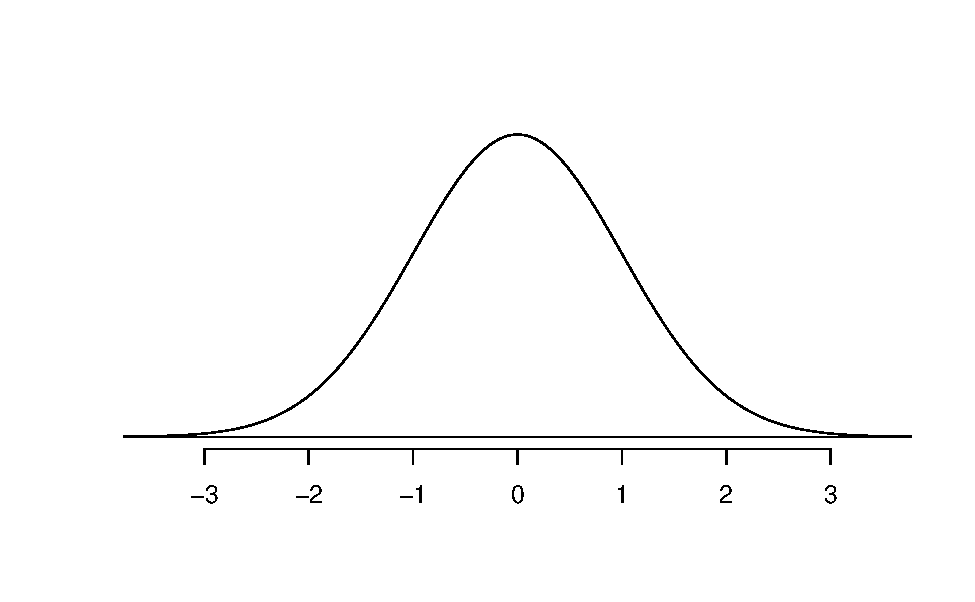
\includegraphics[width=0.6\linewidth]{09-A13-inference-2cat_test-theory_files/figure-latex/simpleNormal-1} 

}

\caption{A standard normal curve.}\label{fig:simpleNormal}
\end{figure}

\begin{enumerate}
\def\labelenumi{\arabic{enumi}.}
\setcounter{enumi}{7}
\tightlist
\item
  Mark the value of the standardized statistic on the standard normal distribution above and shade the area to find the p-value.
\end{enumerate}

\vspace{0.1in}
\newpage

We will use the \texttt{pnorm()} function in R to find the p-value. Use the provided R script file and enter the value of the standardized statistic found in question 7 at \texttt{xx} in line 9; highlight and run lines 9--11.

\begin{Shaded}
\begin{Highlighting}[]
\FunctionTok{pnorm}\NormalTok{(xx, }\CommentTok{\# Enter value of standardized statistic}
      \AttributeTok{m=}\DecValTok{0}\NormalTok{, }\AttributeTok{s=}\DecValTok{1}\NormalTok{, }\CommentTok{\# Using the standard normal mean = 0, sd = 1}
      \AttributeTok{lower.tail=}\ConstantTok{TRUE}\NormalTok{) }\CommentTok{\# Gives a p{-}value less than the standardized statistic}
\end{Highlighting}
\end{Shaded}

\begin{enumerate}
\def\labelenumi{\arabic{enumi}.}
\setcounter{enumi}{8}
\item
  Report the p-value from the R output.
  \vspace{0.2in}
\item
  Interpret the p-value in context of the study.
\end{enumerate}

\vspace{1in}

\begin{enumerate}
\def\labelenumi{\arabic{enumi}.}
\setcounter{enumi}{10}
\tightlist
\item
  Write a conclusion to the research question based on the p-value found.
\end{enumerate}

\vspace{0.8in}

\begin{enumerate}
\def\labelenumi{\arabic{enumi}.}
\setcounter{enumi}{11}
\tightlist
\item
  Would a 90\% confidence interval contain the null value of zero? Explain your answer.
\end{enumerate}

\vspace{0.8in}

\begin{enumerate}
\def\labelenumi{\arabic{enumi}.}
\setcounter{enumi}{12}
\tightlist
\item
  What is the scope of inference for this study?
\end{enumerate}

\newpage

\newpage

\hypertarget{take-home-messages-15}{%
\subsection{Take-home messages}\label{take-home-messages-15}}

\begin{enumerate}
\def\labelenumi{\arabic{enumi}.}
\item
  When comparing two groups, we are looking at the difference between two parameters. In the null hypothesis, we assume the two parameters are equal, or that there is no difference between the two proportions.
\item
  The standardized statistic when the response variable is categorical is a Z-score and is compared to the standard normal distribution to find the p-value. To find the standardized statistic, we take the value of the statistic minus the null value, divided by the null standard error of the statistic. The standardized statistic measures the number of standard errors the statistic is from the null value.
\end{enumerate}

\hypertarget{additional-notes-14}{%
\subsection{Additional notes}\label{additional-notes-14}}

Use this space to summarize your thoughts and take additional notes on today's activity and material covered.

\newpage

\hypertarget{activity-9b-winter-sports-helmet-use-and-head-injuries-theory-based-confidence-interval}{%
\section{Activity 9B: Winter Sports Helmet Use and Head Injuries --- Theory-based Confidence Interval}\label{activity-9b-winter-sports-helmet-use-and-head-injuries-theory-based-confidence-interval}}

\setstretch{1}

\hypertarget{learning-outcomes-18}{%
\subsection{Learning outcomes}\label{learning-outcomes-18}}

\begin{itemize}
\item
  Assess the conditions to use the normal distribution model for a difference in proportions.
\item
  Create and interpret a theory-based confidence interval for a difference in proportions.
\end{itemize}

\hypertarget{terminology-review-16}{%
\subsection{Terminology review}\label{terminology-review-16}}

In today's activity, we will use theory-based methods to estimate the difference in two proportions. Some terms covered in this activity are:

\begin{itemize}
\item
  Standard normal distribution
\item
  Independence and success-failure conditions
\end{itemize}

To review these concepts, see Chapter 15 in your textbook.

\hypertarget{winter-sports-helmet-use-and-head-injury}{%
\subsection{Winter sports helmet use and head injury}\label{winter-sports-helmet-use-and-head-injury}}

In this activity we will focus on theory-based methods to calculate a confidence interval. Recall from Activity 9A, the sampling distribution of a difference in proportions can be mathematically modeled using the normal distribution if certain conditions are met.

Conditions for the sampling distribution of \(\hat{p}_1-\hat{p}_2\) to follow an approximate normal distribution:

\begin{itemize}
\item
  \textbf{Independence}: The data are independent within and between the two groups. (\emph{Remember}: This also must be true to use simulation methods!)
\item
  \textbf{Success-failure condition}: This condition is met if we have at least 10 successes and 10 failures in each sample. Equivalently, we check that all cells in the table have at least 10 observations.
\end{itemize}

\begin{enumerate}
\def\labelenumi{\arabic{enumi}.}
\tightlist
\item
  Explain why a theory-based confidence interval for the data set in Activities 8A and 8B would NOT be similar to the bootstrap interval created.
\end{enumerate}

\vspace{1in}

For this activity we will again use the Helmet Use and Head Injury data set. In Activity 9A we saw that there was evidence that helmet use is assoicated with a reduced risk of head injury. Today we will estimate the difference in proportion of head injuries for those who wore helmets and those who did not.

In ``Helmet Use and Risk of Head Injuries in Alpine Skiers and Snowboarders'' by Sullheim et. al., (Sulheim et al. 2017), we can see the summary results from a random sample of 3562 skiers and snowboarders involved in accidents in the two-way table below.

\begin{longtable}[]{@{}cccc@{}}
\toprule()
& Helmet Use & No Helmet Use & Total \\
\midrule()
\endhead
Head Injury & 96 & 480 & 576 \\
No Head Injury & 656 & 2330 & 2986 \\
Total & 752 & 2810 & 3562 \\
\bottomrule()
\end{longtable}

\begin{enumerate}
\def\labelenumi{\arabic{enumi}.}
\setcounter{enumi}{1}
\tightlist
\item
  Write the parameter of interest for this study in context of the problem.
\end{enumerate}

\vspace{0.8in}

To find a confidence interval for the difference in proportions we will add and subtract the margin of error from the point estimate to find the two endpoints.

\[\hat{p}_1-\hat{p}_2\pm z^*SE(\hat{p}_1-\hat{p}_2), \hspace{.2cm} \text{where}\]
\[SE(\hat{p}_1-\hat{p}_2) = \sqrt{\frac{\hat{p}_1 (1-\hat{p}_1)}{n_1}+\frac{\hat{p}_2 (1-\hat{p}_2)}{n_2}}\]

Note that the formula changes when calculating the variability around the statistic in order to calculate a confidence interval from the formula used in Activity 9A! Here, we use the sample proportions for each group to calculate the standard error for the difference in proportions since we are not assuming that the true difference is zero.

to calculate the standard error for a difference in proportions to create a 90\% confidence interval we substitute in the two sample proportions and the sample size for each group into the equation above.

\[n_1 = 752, n_2 = 2810, \hat{p}_1 = \frac{96}{752} = 0.128, \hat{p}_2 = \frac{480}{2810} = 0.171\]

\[SE(\hat{p}_1-\hat{p}_2) = \sqrt{\frac{0.128 (1-0.128)}{752}+\frac{0.171 (1-0.171)}{2810}} = 0.014\]

Recall that the \(z^*\) multiplier is the percentile of a standard normal distribution that corresponds to our confidence level. If our confidence level is 90\%, we find the Z values that encompass the middle 90\% of the standard normal distribution. If 90\% of the standard normal distribution should be in the middle, that leaves 10\% in the tails, or 5\% in each tail. The \texttt{qnorm()} function in R will tell us the \(z^*\) value for the desired percentile (in this case, 90\% + 5\% = 95\% percentile).

\begin{Shaded}
\begin{Highlighting}[]
\FunctionTok{qnorm}\NormalTok{(}\FloatTok{0.95}\NormalTok{) }\CommentTok{\# Multiplier for 90\% confidence interval}
\end{Highlighting}
\end{Shaded}

\begin{verbatim}
#> [1] 1.644854
\end{verbatim}

\newpage

\begin{enumerate}
\def\labelenumi{\arabic{enumi}.}
\setcounter{enumi}{2}
\tightlist
\item
  Sketch a graph of the standard normal distribution and use the graph to explain how the R code above is used to find the \(z^*\) multiplier.
\end{enumerate}

\vspace{1.5in}

Remember that the margin of error is the value added and subtracted to the sample difference in proportions to find the endpoints for the confidence interval.

\[ME = z^*SE(\hat{p}_1 - \hat{p}_2)\]

\begin{enumerate}
\def\labelenumi{\arabic{enumi}.}
\setcounter{enumi}{3}
\tightlist
\item
  Using the multiplier of \(z^*\) = 1.645 and the standard error calculated above, calculate the margin of error for a 90\% confidence interval.
\end{enumerate}

\vspace{0.5in}

\begin{enumerate}
\def\labelenumi{\arabic{enumi}.}
\setcounter{enumi}{4}
\tightlist
\item
  Calculate the 90\% confidence interval for the parameter of interest.
\end{enumerate}

\vspace{0.8in}

\begin{enumerate}
\def\labelenumi{\arabic{enumi}.}
\setcounter{enumi}{5}
\tightlist
\item
  Interpret the confidence interval found in question 5 in context of the problem.
\end{enumerate}

\vspace{0.8in}

\begin{enumerate}
\def\labelenumi{\arabic{enumi}.}
\setcounter{enumi}{6}
\tightlist
\item
  Interpret the level of confidence in context of the problem. What does it mean to be 90\% confident in the confidence interval?
\end{enumerate}

\vspace{0.8in}

\begin{enumerate}
\def\labelenumi{\arabic{enumi}.}
\setcounter{enumi}{7}
\tightlist
\item
  What decision would you make based on your confidence interval? Explain your answer.
  \vspace{0.5in}
  \newpage
\end{enumerate}

\hypertarget{effect-of-sample-size-1}{%
\subsection{Effect of sample size}\label{effect-of-sample-size-1}}

Suppose in another sample of skiers and snowboards involved in accidents we saw these results:

\begin{longtable}[]{@{}cccc@{}}
\toprule()
& Helmet Use & No Helmet Use & Total \\
\midrule()
\endhead
Head Injury & 135 & 674 & 809 \\
No Head Injury & 921 & 3270 & 4191 \\
Total & 1056 & 3944 & 5000 \\
\bottomrule()
\end{longtable}

Notice that the sample proprotions for each group are the same as the smaller sample size.

\[\hat{p}_1 = \frac{135}{1056}=0.127, \hat{p}_2 = \frac{674}{3944}=0.171\]

\begin{enumerate}
\def\labelenumi{\arabic{enumi}.}
\setcounter{enumi}{8}
\item
  Calculate the standard error for the difference in sample proportions for this new sample.
  \vspace{0.8in}
\item
  Calculate the margin of error for a 90\% confidence interval using a multiplier of \(z^*\) = 1.645 for this new sample. Is the margin of error larger or smaller than the margin of error for the original study?
  \vspace{.8in}
\item
  Calculate the 90\% confidence interval for this new study using the margin of error from question 10.\\
  \vspace{.8in}
\item
  Is the confidence interval calculated in question 11 with the smaller sample size wider or narrower than the confidence interval in question 7? Why?
  \vspace{.8in}
\end{enumerate}

\newpage

\hypertarget{take-home-messages-16}{%
\subsection{Take-home messages}\label{take-home-messages-16}}

\begin{enumerate}
\def\labelenumi{\arabic{enumi}.}
\item
  Simulation-based methods and theory-based methods should give the same results for a study \emph{if the validity conditions are met}. For both methods, observational units need to be independent. To use theory-based methods, additionally, the success-failure condition must be met. Check the validity conditions for each type of test to determine if theory-based methods can be used.
\item
  When calculating the standard error for the difference in sample proportions when doing a hypothesis test, we use the pooled proportion of successes, the best estimate for calculating the variability \emph{under the assumption the null hypothesis is true}. For a confidence interval, we are not assuming a null hypothesis, so we use the values of the two conditional proportions to calculate the standard error. Make note of the difference in these two formulas.
\item
  Increasing sample size will result in less sample-to-sample variability in statistics, which will result in a smaller standard error, and thus a narrower confidence interval.
\end{enumerate}

\hypertarget{additional-notes-15}{%
\subsection{Additional notes}\label{additional-notes-15}}

Use this space to summarize your thoughts and take additional notes on today's activity and material covered.

\newpage

\hypertarget{week-9-lab-diabetes}{%
\section{Week 9 Lab: Diabetes}\label{week-9-lab-diabetes}}

\setstretch{1}

\hypertarget{learning-outcomes-19}{%
\subsection{Learning outcomes}\label{learning-outcomes-19}}

\begin{itemize}
\item
  Given a research question involving two categorical variables, construct the null and alternative hypotheses
  in words and using appropriate statistical symbols.
\item
  Assess the conditions to use the normal distribution model for a difference in proportions.
\item
  Describe and perform a simulation-based hypothesis test for a difference in proportions.
\item
  Calculate the Z test statistic for a difference in proportions.
\item
  Find, interpret, and evaluate the p-value for a hypothesis test for a difference in proportions.
\item
  Create and interpret a theory-based confidence interval for a difference in proportions.
\end{itemize}

\hypertarget{glycemic-control-in-diabetic-adolescents}{%
\subsection{Glycemic control in diabetic adolescents}\label{glycemic-control-in-diabetic-adolescents}}

Researchers compared the efficacy of two treatment regimens to achieve durable glycemic control in children and adolescents with recent-onset type 2 diabetes (Group 2012). A convenience sample of patients 10 to 17 years of age with recent-onset type 2 diabetes were randomly assigned to either a medication (rosiglitazone) or a lifestyle-intervention program focusing on weight loss through eating and activity. Researchers measured whether the patient still needs insulin (failure) or had glycemic control (success). Of the 233 children who received the Rosiglitazone treatment, 143 had glycemic control, while of the 234 who went through the lifestyle-intervention program, 125 had glycemic control. Is there evidence that there is difference in proportion of patients that achieve durable glycemic control between the two treatments? Use Rosiglitazone -- Lifestyle as the order of subtraction.

Upload and open the R script file for Week 9 lab. Upload and import the csv file, \texttt{diabetes}. Enter the name of the data set (see the environment tab) for \texttt{datasetname} in the R script file in line 5. Highlight and run lines 1--6 to get the counts for each combination of categories.

\begin{Shaded}
\begin{Highlighting}[]
\NormalTok{rosi }\OtherTok{\textless{}{-}}\NormalTok{ datasetname}
\NormalTok{rosi }\SpecialCharTok{\%\textgreater{}\%} \FunctionTok{group\_by}\NormalTok{(treatment) }\SpecialCharTok{\%\textgreater{}\%} \FunctionTok{count}\NormalTok{(outcome)}
\end{Highlighting}
\end{Shaded}

\begin{enumerate}
\def\labelenumi{\arabic{enumi}.}
\item
  Is this an experiment or an observational study?
  \vspace{0.2in}
\item
  Complete the following two-way table using the R output.
\end{enumerate}

\begin{center}
\begin{tabular}{|c|c|c|c|}\hline
 & \multicolumn{2}{|c|}{\textbf{Treatment}} & \\ \hline
\textbf{Outcome} & Rosiglitazone & Lifestyle & Total \\ \hline
 Glycemic Control & & & \\ 
 & & & \\ \hline
 Insulin Required & & & \\ 
 & & & \\ \hline
 Total & & &  \\ 
 & & & \\ \hline  
\end{tabular}
\end{center}

\begin{enumerate}
\def\labelenumi{\arabic{enumi}.}
\setcounter{enumi}{2}
\item
  Is the independence condition met for this study? Explain your answer.
  \vspace{0.6in}
\item
  Write the parameter of interest for the research question.
  \vspace{0.6in}
\item
  Using the research question, write the alternative hypothesis in notation.
  \vspace{0.3in}
\item
  \textbf{Calculate the summary statistic (difference in proportions). Use appropriate notation.}
  \vspace{0.3in}
\end{enumerate}

Fill in the missing values/names in the R script file in the two-proportion\_test function to create the null distribution and find the simulation p-value for the test.

\begin{Shaded}
\begin{Highlighting}[]
\FunctionTok{two\_proportion\_test}\NormalTok{(}\AttributeTok{formula =}\NormalTok{ outcome}\SpecialCharTok{\textasciitilde{}}\NormalTok{treatment, }\CommentTok{\# response \textasciitilde{} explanatory}
         \AttributeTok{data=}\NormalTok{ rosi, }\CommentTok{\# Name of data set}
         \AttributeTok{first\_in\_subtraction =} \StringTok{"xx"}\NormalTok{, }\CommentTok{\# Order of subtraction: enter the name of Group 1}
         \AttributeTok{number\_repetitions =} \DecValTok{1000}\NormalTok{, }\CommentTok{\# Always use a minimum of 1000 repetitions}
         \AttributeTok{response\_value\_numerator =} \StringTok{"xx"}\NormalTok{, }\CommentTok{\# Define which outcome is a success }
         \AttributeTok{as\_extreme\_as =}\NormalTok{ xx, }\CommentTok{\# Calculated observed statistic (difference in sample proportions)}
         \AttributeTok{direction=}\StringTok{"xx"}\NormalTok{) }\CommentTok{\# Alternative hypothesis direction ("greater","less","two{-}sided")}
\end{Highlighting}
\end{Shaded}

\begin{enumerate}
\def\labelenumi{\arabic{enumi}.}
\setcounter{enumi}{6}
\item
  Report the p-value. How much evidence does the p-value provide against the null hypothesis?
  \vspace{0.3in}
\item
  \textbf{Will the theory-based p-value be similar to the simulation p-value? Explain your answer.}
  \vspace{0.8in}
\item
  \textbf{Calculate the number of standard errors that sample difference in proportion is from the null value of zero.}
  \vspace{0.8in}
\item
  \textbf{Will a 95\% simulation confidence interval contain the null value of zero? Explain your answer.}
  \vspace{0.8in}
\item
  Calculate the standard error for a difference in proportions to create a 95\% confidence interval.\\
  \vspace{1in}
\item
  Use the multiplier of \(z^*\) = 1.96 and the standard error found in question 11 to calculate a 95\% confidence interval for the parameter of interest.
  \vspace{1in}
\item
  Interpret the confidence interval found in question 12 in context of the problem.
\end{enumerate}

\vspace{0.8in}

\begin{enumerate}
\def\labelenumi{\arabic{enumi}.}
\setcounter{enumi}{13}
\item
  Write a conclusion to the research question.
  \vspace{0.8in}
\item
  Write a paragraph summarizing the results of the study. Be sure to describe:
\end{enumerate}

\begin{itemize}
\item
  Summary statistic and interpretation
\item
  P-value and interpretation
\item
  Confidence interval and interpretation
\item
  Conclusion (written to answer the research question)
\item
  Scope of inference
\end{itemize}

\textbf{Upload a copy of your group's p-value interpretation and scope of inference to Gradescope.}

\newpage

\hypertarget{exam-2-review}{%
\chapter{Exam 2 Review}\label{exam-2-review}}

Use the provided data set from the Islands (ExamReviewData.csv) and the appropriate Exam 2 Review R script file to answer the following questions. Each adult (\textgreater21) islander was selected at random from all adult islanders. Variables and their descriptions are listed below. Music type (classical or heavy metal) was randomly assigned to the Islanders. Time to complete the puzzle cube was measured after listening to music for each Islander. Heart rate and blood glucose levels were both measured before and then after drinking a caffeinated beverage.

\begin{longtable}[]{@{}
  >{\raggedright\arraybackslash}p{(\columnwidth - 2\tabcolsep) * \real{0.2353}}
  >{\raggedright\arraybackslash}p{(\columnwidth - 2\tabcolsep) * \real{0.7647}}@{}}
\toprule()
\begin{minipage}[b]{\linewidth}\raggedright
\textbf{Variable}
\end{minipage} & \begin{minipage}[b]{\linewidth}\raggedright
\textbf{Description}
\end{minipage} \\
\midrule()
\endhead
\texttt{Island} & Name of Island that the Islander resides on \\
\texttt{City} & Name of City in which the Islander resides \\
\texttt{Population} & Population of the City \\
\texttt{Name} & Name of Islander \\
\texttt{Consent} & Whether the Islander consented to be in the study \\
\texttt{Gender} & Gender of Islander (M = male, F = Female) \\
\texttt{Age} & Age of Islander \\
\texttt{Married} & Marital status of Islander \\
\texttt{Smoking\_Status} & Whether the Islander is a current smoker \\
\texttt{Children} & Whether the Islander has children \\
\texttt{weight\_kg} & Weight measured in kg \\
\texttt{height\_cm} & Height measured in cm \\
\texttt{respiratory\_rate} & Breaths per minute \\
\texttt{Type\_of\_Music} & Music type (Classical or Heavy Medal) Islander was randomly assigned to listen to \\
\texttt{After\_PuzzleCube} & Time to complete puzzle cube (minutes) after listening to assigned music \\
\texttt{Education\_Level} & Highest level of education completed \\
\texttt{Balance\_Test} & Time balanced measured in seconds with eyes closed \\
\texttt{Blood\_Glucose\_before} & Level of blood glucose (mg/dL) before consuming assigned drink \\
\texttt{Heart\_Rate\_before} & Heart rate (bpm) before consuming assigned drink \\
\texttt{Blood\_Glucose\_after} & Level of blood glucose (mg/dL) after consuming assigned drink \\
\texttt{Heart\_Rate\_after} & Heart rate (bpm) after consuming assigned drink \\
\texttt{Diff\_Heart\_Rate} & Difference in heart rate (bpm) for Before - After consuming assigned drink \\
\texttt{Diff\_Blood\_Glucose} & Difference in blood glucose (mg/dL) for Before - After consuming assigned drink \\
\bottomrule()
\end{longtable}

\newpage

\begin{enumerate}
\def\labelenumi{\arabic{enumi}.}
\tightlist
\item
  Use the appropriate Exam 2 Review R script file and analyze the following research question: The proportion of university graduates in the US is 42\%. ``Is there evidence that the proportion of university graduates in the Islands differs from the proportion in the US?''
\end{enumerate}

\begin{enumerate}
\def\labelenumi{\alph{enumi}.}
\item
  Parameter of Interest:
  \vspace{0.3in}
\item
  Null Hypothesis:

  Notation:
  \vspace{0.3in}

  Words:
  \vspace{0.5in}
\item
  Alternative Hypothesis:

  Notation:
  \vspace{0.3in}

  Words:
  \vspace{0.5in}
\item
  Use the R script file to get the counts for each level of the variable. Fill in the following table with the success, failure, variable name, and counts using the values from the R output.
\end{enumerate}

\begingroup
\begin{center}
\setlength{\tabcolsep}{14pt} 
\renewcommand{\arraystretch}{2} 
\begin{tabular}{|p{2in}|p{2in}|}
\hline
 {\textbf{Variable}} & {\textbf{Counts}} \\ 
 & \\ \hline
 Success & \\ 
 &  \\ \hline
 Failure & \\ 
 &  \\ \hline
 Total &  \\ 
 & \\ \hline  
\end{tabular}
\end{center}
\endgroup

\begin{enumerate}
\def\labelenumi{\alph{enumi}.}
\setcounter{enumi}{4}
\item
  Calculate the value of summary statistic to answer the research question. Give appropriate notation.
  \vspace{0.3in}
\item
  Interpret the value of the summary statistic in context of the problem:
  \vspace{0.3in}
\item
  Assess if the following conditions are met:

  Independence (needed for both simulation and theory-based methods):
  \vspace{0.8in}

  Success-Failure (must be met to use theory-based methods):
  \vspace{0.8in}
\item
  Use the provided R script file to find the simulation p-value to assess the research question. Report the p-value.
  \vspace{0.3in}
\item
  Interpret the p-value in the context of the problem.
  \vspace{0.8in}
\item
  Write a conclusion to the research question based on the p-value.
  \vspace{0.8in}
\item
  Write a decision based on the p-value.
  \vspace{0.3in}
\item
  Use the provided R script file to find a 90\% confidence interval.
  \vspace{0.3in}
\item
  Interpret the 90\% confidence interval in context of the problem.
  \vspace{0.8in}
\item
  Regardless to your answer in part g, calculate the standardized statistic.
  \vspace{0.4in}
\item
  Interpret the value of the standardized statistic in context of the problem.
  \vspace{0.8in}
\item
  Use the provided R script file to find the theory-based p-value.
  \vspace{0.3in}
\item
  Use the provided R script file to find the appropriate z* multiplier and calculate the theory-based confidence interval.
  \vspace{0.5in}
\item
  Does the theory-based p-value and CI match those found using simulation methods? Explain why or why not.
  \vspace{0.8in}
\item
  To what group can the results be generalized?
  \vspace{0.8in}
\end{enumerate}

\begin{enumerate}
\def\labelenumi{\arabic{enumi}.}
\setcounter{enumi}{1}
\tightlist
\item
  Use the appropriate Exam 2 Review R script file and analyze the following research question: ``Is there evidence that those with a higher education level are less likely to smoke?''
\end{enumerate}

\begin{enumerate}
\def\labelenumi{\alph{enumi}.}
\item
  Parameter of Interest:
  \vspace{0.3in}
\item
  Null Hypothesis:

  Notation:
  \vspace{0.3in}

  Words:
  \vspace{0.5in}
\item
  Alternative Hypothesis:

  Notation:
  \vspace{0.3in}

  Words:
  \vspace{0.5in}
\item
  Use the R script file to get the counts for each level and combination of variables. Fill in the following table with the variable names, levels of each variable, and counts using the values from the R output.
\end{enumerate}

\begingroup
\setlength{\tabcolsep}{14pt}
\renewcommand{\arraystretch}{2}
\begin{center}
\begin{tabular}{|c|p{1in}|p{1in}|p{1in}|}
\hline
 & \multicolumn{2}{|c|}{\textbf{Explanatory Variable}} & \\ 
 & \multicolumn{2}{|c|}{ } & \\ \hline
\textbf{Response variable} & Group 1 & Group 2 & Total \\
 & & & \\ \hline
 Success & & & \\
 & & & \\ \hline
 Failure & & & \\
 & & & \\ \hline
 Total & & & \\
 & & & \\ \hline
\end{tabular}
\end{center}
\endgroup

\begin{enumerate}
\def\labelenumi{\alph{enumi}.}
\setcounter{enumi}{3}
\tightlist
\item
  Calculate the value of summary statistic to answer the research question. Give appropriate notation.
\end{enumerate}

\vspace{0.4in}

\begin{enumerate}
\def\labelenumi{\alph{enumi}.}
\setcounter{enumi}{4}
\tightlist
\item
  Interpret the value of the summary statistic in context of the problem:
\end{enumerate}

\vspace{0.4in}

\begin{enumerate}
\def\labelenumi{\alph{enumi}.}
\setcounter{enumi}{6}
\item
  Assess if the following conditions are met:

  Independence (needed for both simulation and theory-based methods):
  \vspace{0.8in}

  Success-Failure (must be met to use theory-based methods):
  \vspace{0.8in}
\item
  Use the provided R script file to find the simulation p-value to assess the research question. Report the p-value.
  \vspace{0.3in}
\item
  Interpret the p-value in the context of the problem.
  \vspace{0.8in}
\item
  Write a conclusion to the research question based on the p-value.
  \vspace{0.8in}
\item
  Write a decision based on the p-value.
  \vspace{0.3in}
\item
  Use the provided R script file to find a 95\% confidence interval.
  \vspace{0.3in}
\item
  Interpret the 95\% confidence interval in context of the problem.
  \vspace{0.8in}
\item
  Regardless to your answer in part g, calculate the standardized statistic.
  \vspace{0.4in}
\item
  Interpret the value of the standardized statistic in context of the problem.
  \vspace{0.8in}
\item
  Use the provided R script file to find the theory-based p-value.
  \vspace{0.3in}
\item
  Use the provided R script file to find the appropriate z* multiplier and calculate the theory-based confidence interval.
  \vspace{0.5in}
\item
  Does the theory-based p-value and CI match those found using simulation methods? Explain why or why not.
  \vspace{0.8in}
\item
  What is the scope of inference for this study?
  \vspace{0.8in}
\end{enumerate}

\newpage

\hypertarget{inference-for-a-quantitative-response-with-paired-samples}{%
\chapter{Inference for a Quantitative Response with Paired Samples}\label{inference-for-a-quantitative-response-with-paired-samples}}

\hypertarget{week-11-reading-guide-inference-for-a-single-mean-or-paired-mean-difference}{%
\section{Week 11 Reading Guide: Inference for a Single Mean or Paired Mean Difference}\label{week-11-reading-guide-inference-for-a-single-mean-or-paired-mean-difference}}

\hypertarget{chapter-17-inference-for-a-single-mean}{%
\subsection*{Chapter 17 (Inference for a single mean)}\label{chapter-17-inference-for-a-single-mean}}
\addcontentsline{toc}{subsection}{Chapter 17 (Inference for a single mean)}

\textbf{Videos}

\begin{itemize}
\tightlist
\item
  17.1
\item
  17.2
\item
  17.3Tests
\item
  17.4Intervals
\end{itemize}

\setstretch{1.25}

\hypertarget{reminders-from-previous-sections-9}{%
\subsubsection*{Reminders from previous sections}\label{reminders-from-previous-sections-9}}
\addcontentsline{toc}{subsubsection}{Reminders from previous sections}

\(n\) = sample size

\(\overline{x}\) = sample mean

\(s\) = sample standard deviation

\(\mu\) = population mean

\(\sigma\) = population standard deviation

General steps of a hypothesis test:

\begin{enumerate}
\def\labelenumi{\arabic{enumi}.}
\item
  Frame the research question in terms of hypotheses.
\item
  Collect and summarize data using a test statistic.
\item
  Assume the null hypothesis is true, and simulate or mathematically model a null distribution for the test statistic.
\item
  Compare the observed test statistic to the null distribution to calculate a p-value.
\item
  Make a conclusion based on the p-value and write the conclusion in context.
\end{enumerate}

Parameter: a value summarizing a variable(s) for a population.

Statistic: a value summarizing a variable(s) for a sample.

Sampling distribution: plot of statistics from 1000s of samples of the same size taken from the same population.

Standard deviation of a statistic: the variability of statistics from 1000s of samples; how far, on average, each statistic is from the true value of the parameter.

Standard error of a statistic: estimated standard deviation of a statistic.

Hypothesis test: a process to determine how strong the evidence of an effect is. Also called a `significance test'.

Simulation-based method: Simulate lots of samples of size \(n\) under assumption of the null hypothesis, then find the proportion of the simulations that are at least as extreme as the observed sample statistic.

Theory-based method: Develop a mathematical model for the sampling distribution of the statistic under the null hypothesis and use the model to calculate the probability of the observed sample statistic (or one more extreme) occurring.

Null hypothesis (\(H_0\)): the skeptical perspective; no difference; no change; no effect; random chance; what the researcher hopes to prove is \textbf{wrong}.

Alternative hypothesis (\(H_A\)): the new perspective; a difference/increase/decrease; an effect; not random chance; what the researcher hopes to prove is \textbf{correct}.

Null value: the value of the parameter when we assume the null hypothesis is true (labeled as \(parameter_0\)).

Null distribution: the simulated or modeled distribution of statistics (sampling distribution) we would expect to occur if the null hypothesis is true.

P-value: probability of seeing the observed sample data, or something more extreme, assuming the null hypothesis is true.

\(\implies\) Lower the p-value the stronger the evidence AGAINST the null hypothesis and FOR the alternative hypothesis.

Decision: a determination of whether to reject or fail to reject a null hypothesis based on a p-value and a pre-set level of significance.

\begin{itemize}
\item
  If p-value \(\leq \alpha\), then reject \(H_0\).
\item
  If p-value \(> \alpha\), then fail to reject \(H_0\).
\end{itemize}

Significance level (\(\alpha\)): a threshold used to determine if a p-value provides enough evidence to reject the null hypothesis or not.

\rgi Common levels of \(\alpha\) include 0.01, 0.05, and 0.10.

Statistically significant: results are considered statistically significant if the p-value is below the significance level.

Confidence interval: a process to determine how large an effect is; a range of plausible values for the parameter. Also called `estimation'.

Margin of error: the value that is added to and subtracted from the sample statistic to create a confidence interval; half the width of a confidence interval.

Bootstrapping: the process of drawing with replacement \(n\) times from the original sample.

Bootstrapped resample: a random sample of size \(n\) from the original sample, selected with replacement.

Bootstrapped statistic: the statistic recorded from the bootstrapped resample.

Confidence level: how confident we are that the confidence interval will capture the parameter.

Bootstrap \(X\)\% confidence interval: (\((\frac{(1-X)}{2})^{th}\) percentile, \((X+(\frac{(1-X)}{2})^{th}\) percentile) of a bootstrap distribution.

Central Limit Theorem: For large sample sizes, the sampling distribution of a sample mean (or proportion) will be approximately normal (bell-shaped and symmetric).

\hypertarget{vocabulary-17}{%
\subsubsection*{Vocabulary}\label{vocabulary-17}}
\addcontentsline{toc}{subsubsection}{Vocabulary}

Shifted bootstrap test:
\rgs

\(t\)-distribution:
\rgs 

\begin{itemize}
\item
  The variability in the \(t\)-distribution depends on the sample size (used to calculate degrees of freedom --- df for short).
\item
  The larger df, the closer the \(t\) distribution is to the standard normal distribution.
\end{itemize}

Degrees of freedom (df):
\rgs 

T-score:
\rgs 

\hypertarget{notes-22}{%
\subsubsection*{Notes}\label{notes-22}}
\addcontentsline{toc}{subsubsection}{Notes}

To create a shifted bootstrap distribution test,

\rgi How many cards will you need and how will the cards be labeled?
\rgs 

\rgi Why are the data values shifted prior to being written on the cards?
\rgs

\rgi What do you do with the cards after labeling them?
\rgs 

\rgi After resampling, what value will be plotted on the bootstrap distribution?
\rgs 

True or false: Bootstrapping can only be used if the sample size is small.
\rgs 

Why do we use a \(t\)-distribution rather than the normal distribution when analyzing quantitative data?
\rgs 

How do we calculate degrees of freedom for the \(t\)-distribution?
\rgs 

Conditions to use the CLT for means:

\rgi Independence:
\rgs 

\rgi \rgi Checked by:
\rgs 

\rgi Normality:
\rgs 

\rgi \rgi Checked by:
\rgs 

\hypertarget{formulas-3}{%
\subsubsection*{Formulas}\label{formulas-3}}
\addcontentsline{toc}{subsubsection}{Formulas}

\(SE(\overline{x})=\)
\rgs 

\(T=\)
\rgs 

Confidence interval for a single mean:
\rgs 

\hypertarget{notation-2}{%
\subsubsection*{Notation}\label{notation-2}}
\addcontentsline{toc}{subsubsection}{Notation}

\(\mu_0\) represents
\rgs 

\hypertarget{example-from-section-17.1-edinburgh-rentals}{%
\subsubsection*{Example from section 17.1: Edinburgh rentals}\label{example-from-section-17.1-edinburgh-rentals}}
\addcontentsline{toc}{subsubsection}{Example from section 17.1: Edinburgh rentals}

\begin{enumerate}
\def\labelenumi{\arabic{enumi}.}
\item
  What are the observational units?
  \rgs 
\item
  What are the sample statistics presented in this example? What notation would be used to represent each value?
  \rgs 
\item
  What is the parameter representing in the context of this problem? What notation would be used to represent this parameter?
  \rgs 
  \rgs 
\item
  How could we use cards to simulate \textbf{one} bootstrap resample \emph{which does not assume the null hypothesis is true}? How many cards? What is written on the cards? What would we do with the cards? What would you record once you have a simulated sample?
  \rgs 
  \rgs 
  \rgs 
\item
  After 1000 resamples are generated, where is the resulting bootstrap distribution centered? Why does that make sense?
  \rgs 
  \rgs 
\item
  Based on Figure 17.3, give the confidence interval for the true mean for each of the following confidence levels.
\end{enumerate}

\rgi 90\% confidence interval =
\rgs 

\rgi 95\% confidence interval =
\rgs 

\rgi 99\% confidence interval =
\rgs 

\begin{enumerate}
\def\labelenumi{\arabic{enumi}.}
\setcounter{enumi}{6}
\tightlist
\item
  Interpret your 99\% confidence interval in the context of the problem.
  \rgs 
  \rgs 
\end{enumerate}

\hypertarget{example-from-section-17.2-sleep-times-of-msu-students}{%
\subsubsection*{Example from section 17.2: Sleep times of MSU students}\label{example-from-section-17.2-sleep-times-of-msu-students}}
\addcontentsline{toc}{subsubsection}{Example from section 17.2: Sleep times of MSU students}

\begin{enumerate}
\def\labelenumi{\arabic{enumi}.}
\item
  What is the research question?
  \rgs
\item
  What are the observational units?
  \rgs
\item
  Can the results of this study be generalized to a larger population? Why or why not?
  \rgs
\item
  What are the sample statistics presented in this example? What notation would be used to represent each value?
  \rgs
\item
  What is the parameter representing in the context of this problem? What notation would be used to represent this parameter?
  \rgs
  \rgs
\item
  Write the null and the alternative hypotheses in words.
  \rgs
  \rgs
\item
  Write the null and the alternative hypotheses in notation.
  \rgs
\item
  How could we use cards to simulate \textbf{one} shifted bootstrap resample \emph{which assumes the null hypothesis is true}? How many cards? What is written on the cards (be sure to include the amount and direction of the shift)? What would we do with the cards? What would you record once you have a simulated sample?
  \rgs 
  \rgs 
  \rgs 
\item
  What was the p-value of the test?
  \rgs
\item
  Interpret the p-value in the context of the problem.
  \rgs
  \rgs
\item
  At the 5\% significance level, what decision would you make? What type of error might that be?
  \rgs
\item
  What conclusion should the researcher make?
  \rgs
  \rgs
\item
  Are the results in this example statistically significant? Justify your answer.
  \rgs
\end{enumerate}

\hypertarget{example-from-section-17.3-mercury-content-of-dolphin-muscle}{%
\subsubsection*{Example from section 17.3: Mercury content of dolphin muscle}\label{example-from-section-17.3-mercury-content-of-dolphin-muscle}}
\addcontentsline{toc}{subsubsection}{Example from section 17.3: Mercury content of dolphin muscle}

\begin{enumerate}
\def\labelenumi{\arabic{enumi}.}
\item
  What is the research question?
  \rgs 
\item
  What are the observational units?
  \rgs 
\item
  Can the results of this study be generalized to a larger population? Why or why not?
  \rgs 
\item
  What are the sample statistics presented in this example? What notation would be used to represent each value?
  \rgs 
\item
  What is the parameter representing in the context of this problem? What notation would be used to represent this parameter?
  \rgs 
  \rgs 
\item
  Are the independence and normality conditions satisfied?
  \rgs 
  \rgs 
\item
  Calculate the standard error of the sample mean.
  \rgs 
  \rgs
\item
  What distribution should be referenced to find the multiplier for a 95\% confidence interval?
  \rgs 
\item
  Using \(t^\star=2.10\), calculate a 95\% confidence interval for \(\mu\).
  \rgs 
  \rgs
\item
  Interpret the interval calculated in the context of the problem.
  \rgs 
  \rgs 
\end{enumerate}

\hypertarget{example-from-section-17.3-cherry-blossom-race}{%
\subsubsection*{Example from section 17.3: Cherry Blossom Race}\label{example-from-section-17.3-cherry-blossom-race}}
\addcontentsline{toc}{subsubsection}{Example from section 17.3: Cherry Blossom Race}

\begin{enumerate}
\def\labelenumi{\arabic{enumi}.}
\item
  What is the research question?
  \rgs
\item
  What are the observational units?
  \rgs
\item
  Can the results of this study be generalized to a larger population? Why or why not?
  \rgs
\item
  What are the sample statistics presented in this example? What notation would be used to represent each value?
  \rgs
\item
  What is the parameter representing in the context of this problem? What notation would be used to represent this parameter?
  \rgs
  \rgs
\item
  Are the independence and normality conditions satisfied?
  \rgs
  \rgs
\item
  Write the null and the alternative hypotheses in words.
  \rgs
  \rgs
\item
  Write the null and the alternative hypotheses in notation.
  \rgs
\item
  Calculate the standard error of the sample mean.
  \rgs
  \rgs
\item
  Calculate the T-score (the standardized statistic for the sample mean).
  \rgs
  \rgs
\item
  What distribution should the T-score be compared to in order to calculate a p-value?
  \rgs
\item
  What was the p-value of the test?
  \rgs
\item
  Interpret the p-value in the context of the problem.
  \rgs
  \rgs
\item
  At the 5\% significance level, what decision would you make? What type of error might that be?
  \rgs
\item
  What conclusion should the researcher make?
  \rgs
  \rgs
\item
  Are the results in this example statistically significant? Justify your answer.
  \rgs
\end{enumerate}

\hypertarget{chapter-18-inference-for-paired-mean-difference}{%
\subsection*{Chapter 18 (Inference for paired mean difference)}\label{chapter-18-inference-for-paired-mean-difference}}
\addcontentsline{toc}{subsection}{Chapter 18 (Inference for paired mean difference)}

\setstretch{1}

\textbf{Videos}

\begin{itemize}
\tightlist
\item
  Paired\_Data
\item
  18.1and18.2
\item
  18.3
\end{itemize}

\setstretch{1.25}

\hypertarget{vocabulary-18}{%
\subsubsection*{Vocabulary}\label{vocabulary-18}}
\addcontentsline{toc}{subsubsection}{Vocabulary}

Paired data:
\rgs

\rgi Paired with repeated measures:
\rgs

\rgi Paired with matching:
\rgs

\hypertarget{notes-23}{%
\subsubsection*{Notes}\label{notes-23}}
\addcontentsline{toc}{subsubsection}{Notes}

For each of the following scenarios, determine if the two sets of observations are paired or independent.

\begin{enumerate}
\def\labelenumi{\arabic{enumi}.}
\item
  To test whether the IQ is related to genetics, researchers measured the IQ of two biological parents and the IQ of their first-born child. The average parent IQ was compared to the IQ of the first born child.
  \rgs
\item
  Hoping to see how exercise is related to heart rates, researchers asked a group of 30 volunteers to do either bicycle kicks or jumping jacks for 30 seconds. Each volunteer's heart rate was measured at the end of 30 seconds, then the volunteer sat for a 5 minute rest period. At the end of the rest period, the volunteer performed the other activity and their heart rate was measured again. Which activity was done first was randomly assigned.
  \rgs
\item
  Researchers hoping to look into the effectiveness of blended learning gathered two random samples of 50 8th graders (one at Belgrade Middle School which had 5 full-day instruction at the time of the study, the other from Chief Joseph Middle School which utilized a 2-day on, 3-day off blended learning structure). All 8th graders were given the same lessons and same homework, then asked to take the same end-of-unit test.
  \rgs
\end{enumerate}

Conditions to use the CLT for paired mean difference:

\rgi Independence:
\rgs

\rgi \rgi Checked by:
\rgs 

\rgi Normality:
\rgs

\rgi \rgi Checked by:
\rgs

\hypertarget{formulas-4}{%
\subsubsection*{Formulas}\label{formulas-4}}
\addcontentsline{toc}{subsubsection}{Formulas}

\(SE(\overline{x_d})=\)
\rgs

\(T=\)
\rgs

Confidence interval for a paired mean difference:
\rgs

\hypertarget{notation-3}{%
\subsubsection*{Notation}\label{notation-3}}
\addcontentsline{toc}{subsubsection}{Notation}

\(\overline{x_d}=\)
\rgs

\(s_d=\)
\rgs

\(\mu_d=\)
\rgs

\(\sigma_d=\)
\rgs

\hypertarget{example-from-section-18.1-tires}{%
\subsubsection*{Example from section 18.1: Tires}\label{example-from-section-18.1-tires}}
\addcontentsline{toc}{subsubsection}{Example from section 18.1: Tires}

\begin{enumerate}
\def\labelenumi{\arabic{enumi}.}
\item
  What are the observational units?
  \rgs
\item
  Why should we treat these data as paired rather than two independent samples?
  \rgs
\item
  What are the sample statistics presented in this example? What notation would be used to represent each value?
  \rgs
\item
  What is the parameter representing in the context of this problem? What notation would be used to represent this parameter?
  \rgs
  \rgs
\item
  Write the null and alternative hypotheses in appropriate notation.
  \rgs
\item
  How could we use cards to simulate \textbf{one} shifted bootstrap resample \emph{which assumes the null hypothesis is true}? How many cards? What is written on the cards? What would we do with the cards? What would you record once you have a simulated sample?
  \rgs
  \rgs
  \rgs
\item
  After 1000 resamples are generated, where is the resulting null distribution centered? Why does that make sense?
  \rgs
\item
  What was the p-value of the test? Interpret this p-value in the context of the problem.
  \rgs
  \rgs
\item
  Write a conclusion in the context of the problem.
  \rgs
\end{enumerate}

\hypertarget{example-from-sections-18.2-and-18.3-ucla-textbook-prices}{%
\subsubsection*{Example from sections 18.2 and 18.3: UCLA textbook prices}\label{example-from-sections-18.2-and-18.3-ucla-textbook-prices}}
\addcontentsline{toc}{subsubsection}{Example from sections 18.2 and 18.3: UCLA textbook prices}

\begin{enumerate}
\def\labelenumi{\arabic{enumi}.}
\item
  What is the research question?
  \rgs
\item
  What are the observational units?
  \rgs
\item
  Why should we treat these data as paired rather than two independent samples?
  \rgs
\item
  What are the sample statistics presented in this example? What notation would be used to represent each value?
  \rgs
\item
  What is the parameter representing in the context of this problem? What notation would be used to represent this parameter?
  \rgs
  \rgs
\item
  How could we use cards to simulate \textbf{one} bootstrap resample \emph{which does not assume the null hypothesis is true}? How many cards? What is written on the cards? What would we do with the cards? What would you record once you have a simulated sample?
  \rgs
  \rgs
  \rgs
\item
  After 1000 resamples are generated, where is the resulting bootstrap distribution centered? Why does that make sense?
  \rgs
  \rgs
\item
  Give the 95\% confidence interval for \(\mu_d\).
  \rgs
\item
  Interpret your 95\% confidence interval in the context of the problem.
  \rgs
  \rgs
\item
  Are the independence and normality conditions satisfied?
  \rgs
  \rgs
\item
  Write the null and the alternative hypotheses in words.
  \rgs
  \rgs
\item
  Calculate the standard error of the sample mean difference.
  \rgs
  \rgs
\item
  Calculate the T-score (the standardized statistic for the sample mean difference).
  \rgs
  \rgs
\item
  What distribution should the T-score be compared to in order to calculate a p-value?
  \rgs
\item
  What was the p-value of the test?
  \rgs
\item
  At the 5\% significance level, what decision would you make? What type of error might that be?
  \rgs
\item
  What conclusion should the researcher make?
  \rgs
  \rgs
\item
  Are the results in this example statistically significant? Justify your answer.
  \rgs
\item
  Using \(t^\star=2.00\), calculate a 95\% confidence interval for \(\mu_d\).
  \rgs
  \rgs
\item
  Interpret the interval calculated in the context of the problem.
  \rgs
  \rgs
\end{enumerate}

\newpage

\hypertarget{activity-11a-covid-19-and-air-pollution}{%
\section{Activity 11A: COVID-19 and Air Pollution}\label{activity-11a-covid-19-and-air-pollution}}

\setstretch{1}

\hypertarget{learning-outcomes-20}{%
\subsection{Learning outcomes}\label{learning-outcomes-20}}

\begin{itemize}
\item
  Given a research question involving paired differences, construct the null and alternative hypotheses
  in words and using appropriate statistical symbols.
\item
  Describe and perform a simulation-based hypothesis test for a paired mean difference.
\item
  Interpret and evaluate a p-value for a simulation-based hypothesis test for a paired mean difference.
\item
  Use bootstrapping to find a confidence interval for a paired mean difference.
\item
  Interpret a confidence interval for a paired mean difference.
\item
  Use a confidence interval to determine the conclusion of a hypothesis test.
\end{itemize}

\hypertarget{terminology-review-17}{%
\subsection{Terminology review}\label{terminology-review-17}}

In today's activity, we will analyze paired quantitative data using simulation-based methods. Some terms covered in this activity are:

\begin{itemize}
\item
  Mean difference
\item
  Paired data
\item
  Independent groups
\item
  Shifted bootstrap (null) distribution
\end{itemize}

To review these concepts, see Section 18 in the textbook.

\hypertarget{covid-19-and-air-pollution}{%
\subsection{COVID-19 and air pollution}\label{covid-19-and-air-pollution}}

In June 2020, the social distancing efforts and stay-at-home directives to help combat the spread of COVID-19 appeared to help `flatten the curve' across the United States, albeit at a high cost to many individuals and businesses. The impact of these measures, though, goes far beyond the infection and death rates from the disease. You may have seen images comparing air quality in large international cities like Rome, Milan, Wuhan, and New Delhi such as the one pictured in Figure \ref{fig:covid}, which seem to indicate, perhaps unsurprisingly, that fewer people driving and factories being shut down have reduced air pollutants.

Have high population-density US cities seen the same improved air quality conditions? To study this question, data were gathered from the US Environmental Protection Agency (EPA) AirData website which records the ozone (O3) and fine particulate matter (PM2.5) values for cities across the US (US Environmental Protection Agency, n.d.). These measures are used to calculate an air quality index (AQI) score for each city each day of the year. Thirty-three of the most densely populated US cities were selected and the AQI score recorded for April 20, 2020 as well as the five-year median AQI score for April 20th (2015--2019). Note that higher AQI scores indicate worse air quality. A box plot of the differences in AQI scores for the 33 cities and a table of summary statistics are shown on the next page. Use Current - 5-year median as the order of subtraction.

\begin{figure}

{\centering 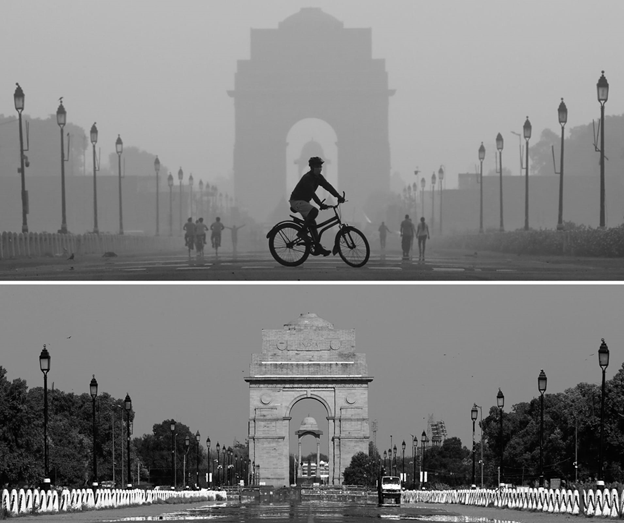
\includegraphics[width=0.6\linewidth]{images/air_pollution_greyscale} 

}

\caption{The India Gate in New Delhi, India.}\label{fig:covid}
\end{figure}

\vspace{.05in}

\begin{center}\includegraphics[width=0.6\linewidth]{11-A15-paired-simulation_files/figure-latex/unnamed-chunk-2-1} \end{center}

\vspace{.2in}

\begin{longtable}[]{@{}
  >{\centering\arraybackslash}p{(\columnwidth - 6\tabcolsep) * \real{0.2143}}
  >{\centering\arraybackslash}p{(\columnwidth - 6\tabcolsep) * \real{0.3143}}
  >{\raggedright\arraybackslash}p{(\columnwidth - 6\tabcolsep) * \real{0.2857}}
  >{\raggedright\arraybackslash}p{(\columnwidth - 6\tabcolsep) * \real{0.1857}}@{}}
\caption{Summary statistics for current AQI scores, median AQI scores from 2015--2019, and the differences in AQI scores.}\tabularnewline
\toprule()
\begin{minipage}[b]{\linewidth}\centering
\end{minipage} & \begin{minipage}[b]{\linewidth}\centering
Mean
\end{minipage} & \begin{minipage}[b]{\linewidth}\raggedright
Standard deviation
\end{minipage} & \begin{minipage}[b]{\linewidth}\raggedright
Sample size
\end{minipage} \\
\midrule()
\endfirsthead
\toprule()
\begin{minipage}[b]{\linewidth}\centering
\end{minipage} & \begin{minipage}[b]{\linewidth}\centering
Mean
\end{minipage} & \begin{minipage}[b]{\linewidth}\raggedright
Standard deviation
\end{minipage} & \begin{minipage}[b]{\linewidth}\raggedright
Sample size
\end{minipage} \\
\midrule()
\endhead
Current & \(\bar{x}_1\) = 47.394 & \(s_1\) = 14.107 & \(n_1\) = 33 \\
5 Year Median & \(\bar{x}_2\) = 51.545 & \(s_2\) = 17.447 & \(n_2\) = 33 \\
Differences & \(\bar{x}_d\) = \(-4.152\) & \(s_d\) = 17.096 & \(n_d\) = 33 \\
\bottomrule()
\end{longtable}

\newpage

\hypertarget{vocabulary-review.}{%
\subsubsection*{Vocabulary review.}\label{vocabulary-review.}}
\addcontentsline{toc}{subsubsection}{Vocabulary review.}

\begin{enumerate}
\def\labelenumi{\arabic{enumi}.}
\tightlist
\item
  Identify the variables in this study. What role (explanatory or response) do each have?
\end{enumerate}

\vspace{.5in}

\begin{enumerate}
\def\labelenumi{\arabic{enumi}.}
\setcounter{enumi}{1}
\tightlist
\item
  Are the differences in AQI scores independent for each case (US city)? Explain.
\end{enumerate}

\vspace{0.5in}

\begin{enumerate}
\def\labelenumi{\arabic{enumi}.}
\setcounter{enumi}{2}
\tightlist
\item
  Why is this treated as a paired study design and not two independent samples?
\end{enumerate}

\vspace{0.5in}

\hypertarget{ask-a-research-question-2}{%
\subsubsection*{Ask a research question}\label{ask-a-research-question-2}}
\addcontentsline{toc}{subsubsection}{Ask a research question}

\begin{enumerate}
\def\labelenumi{\arabic{enumi}.}
\setcounter{enumi}{3}
\tightlist
\item
  Write the null hypothesis in words.
\end{enumerate}

\vspace{0.8in}

\begin{enumerate}
\def\labelenumi{\arabic{enumi}.}
\setcounter{enumi}{4}
\tightlist
\item
  What is the research question?
\end{enumerate}

\vspace{0.8in}

\begin{enumerate}
\def\labelenumi{\arabic{enumi}.}
\setcounter{enumi}{5}
\tightlist
\item
  Write the alternative hypothesis in notation.
\end{enumerate}

\vspace{0.3in}

\hypertarget{summarize-and-visualize-the-data-2}{%
\subsubsection*{Summarize and visualize the data}\label{summarize-and-visualize-the-data-2}}
\addcontentsline{toc}{subsubsection}{Summarize and visualize the data}

\begin{enumerate}
\def\labelenumi{\arabic{enumi}.}
\setcounter{enumi}{6}
\tightlist
\item
  Report the summary statistic of interest (mean difference) for the data.
\end{enumerate}

\vspace{0.3in}

\begin{enumerate}
\def\labelenumi{\arabic{enumi}.}
\setcounter{enumi}{7}
\tightlist
\item
  What notation is used for the value in question 7?
\end{enumerate}

\vspace{0.3in}

\hypertarget{use-statistical-inferential-methods-to-draw-inferences-from-the-data}{%
\subsubsection*{Use statistical inferential methods to draw inferences from the data}\label{use-statistical-inferential-methods-to-draw-inferences-from-the-data}}
\addcontentsline{toc}{subsubsection}{Use statistical inferential methods to draw inferences from the data}

\hypertarget{hypothesis-test}{%
\paragraph*{Hypothesis test}\label{hypothesis-test}}
\addcontentsline{toc}{paragraph}{Hypothesis test}

To simulate the null distribution of paired sample mean differences we will use a bootstrapping method. Recall that the null distribution must be created under the assumption that the null hypothesis is true. Therefore, before bootstrapping, we will need to \emph{shift} each data point by the difference \(\mu_0 - \bar{x}_d\). This will ensure that the mean of the shifted data is \(\mu_0\) (rather than the mean of the original data, \(\bar{x}_d\)), and that the simulated null distribution will be centered at the null value.

\begin{enumerate}
\def\labelenumi{\arabic{enumi}.}
\setcounter{enumi}{8}
\tightlist
\item
  Calculate the difference \(\mu_0 - \bar{x}_d\). Will we need to shift the data up or down?
\end{enumerate}

\vspace{.7in}

We will use the \texttt{paired\_test()} function in R (in the \texttt{catstats} package) to simulate the shifted bootstrap (null) distribution of sample mean differences and compute a p-value. Use the provided R script file and enter the calculated value from question 9 for \texttt{xx} to simulate the null distribution and enter the summary statistic from question 7 for \texttt{yy} to find the p-value. Highlight and run lines 1--21.

\begin{Shaded}
\begin{Highlighting}[]
    \FunctionTok{paired\_test}\NormalTok{(}\AttributeTok{data =}\NormalTok{ Air}\SpecialCharTok{$}\NormalTok{Difference,   }\CommentTok{\# Vector of differences }
                                         \CommentTok{\# or data set with column for each group}
            \AttributeTok{shift =}\NormalTok{ xx,   }\CommentTok{\# Shift needed for bootstrap hypothesis test}
            \AttributeTok{as\_extreme\_as =}\NormalTok{ yy,  }\CommentTok{\# Observed statistic}
            \AttributeTok{direction =} \StringTok{"less"}\NormalTok{,  }\CommentTok{\# Direction of alternative}
            \AttributeTok{number\_repetitions =} \DecValTok{1000}\NormalTok{,  }\CommentTok{\# Number of simulated samples for null distribution}
            \AttributeTok{which\_first =} \DecValTok{1}\NormalTok{)  }\CommentTok{\# Not needed when using calculated differences}
\end{Highlighting}
\end{Shaded}

\begin{enumerate}
\def\labelenumi{\arabic{enumi}.}
\setcounter{enumi}{9}
\tightlist
\item
  Sketch the null distribution created using the R output here.
\end{enumerate}

\vspace{1.8in}

\begin{enumerate}
\def\labelenumi{\arabic{enumi}.}
\setcounter{enumi}{10}
\tightlist
\item
  Explain why the null distribution is centered at zero.
\end{enumerate}

\vspace{.5in}

\begin{enumerate}
\def\labelenumi{\arabic{enumi}.}
\setcounter{enumi}{11}
\item
  What proportion of samples are at or less than the observed sample mean difference in AQI scores for current scores minus 5 year median scores? What is the statistical term for this proportion?
  \vspace{.3in}
\item
  Interpret the p-value in the context of the problem.
  \vspace{.8in}
\item
  How much evidence does this provide for improved air quality in US cities?
  \vspace{.3in}
\item
  If evidence was found for improved air quality in US cities, could we conclude that the stay-at-home directives \emph{caused} the improvement in air quality? Explain.
  \vspace{.5in}
\end{enumerate}

\hypertarget{confidence-interval}{%
\paragraph*{Confidence interval}\label{confidence-interval}}
\addcontentsline{toc}{paragraph}{Confidence interval}

We will use the \texttt{paired\_bootstrap\_CI()} function in R (in the \texttt{catstats} package) to simulate the bootstrap distribution of sample mean differences and calculate a confidence interval.

\begin{enumerate}
\def\labelenumi{\arabic{enumi}.}
\setcounter{enumi}{15}
\tightlist
\item
  Write out the parameter of interest in context of the study.
\end{enumerate}

\vspace{0.8in}

\begin{enumerate}
\def\labelenumi{\arabic{enumi}.}
\setcounter{enumi}{16}
\tightlist
\item
  Using the provided R script file, fill in the missing value at \texttt{xx} to find a 99\% bootstrap confidence interval; highlight and run lines 24--27. Report the confidence interval in interval notation.
\end{enumerate}

\begin{Shaded}
\begin{Highlighting}[]
\FunctionTok{paired\_bootstrap\_CI}\NormalTok{(}\AttributeTok{data =}\NormalTok{ Air}\SpecialCharTok{$}\NormalTok{Difference, }\CommentTok{\# Enter vector of differences}
                    \AttributeTok{number\_repetitions =} \DecValTok{1000}\NormalTok{, }\CommentTok{\# Number of bootstrap samples for CI}
                    \AttributeTok{confidence\_level =}\NormalTok{ xx,  }\CommentTok{\# Confidence level in decimal form}
                    \AttributeTok{which\_first =} \DecValTok{1}\NormalTok{)  }\CommentTok{\# Not needed when entering vector of differences}
\end{Highlighting}
\end{Shaded}

\vspace{.5in}

\hypertarget{communicate-the-results-and-answer-the-research-question-2}{%
\subsubsection*{Communicate the results and answer the research question}\label{communicate-the-results-and-answer-the-research-question-2}}
\addcontentsline{toc}{subsubsection}{Communicate the results and answer the research question}

\begin{enumerate}
\def\labelenumi{\arabic{enumi}.}
\setcounter{enumi}{17}
\tightlist
\item
  Interpret the 99\% confidence interval in the context of the problem.
\end{enumerate}

\vspace{0.7in}

\begin{enumerate}
\def\labelenumi{\arabic{enumi}.}
\setcounter{enumi}{18}
\tightlist
\item
  Do the results of your confidence interval and hypothesis test agree? What does each tell you about the null hypothesis?
\end{enumerate}

\vspace{.7in}

\hypertarget{take-home-messages-17}{%
\subsection{Take-home messages}\label{take-home-messages-17}}

\begin{enumerate}
\def\labelenumi{\arabic{enumi}.}
\item
  The differences in a paired data set are treated like a single quantitative variable when performing a statistical analysis. Paired data (or paired samples) occur when pairs of measurements are collected. We are only interested in the population (and sample) of differences, and not in the original data.
\item
  When using bootstrapping to create a null distribution centered at the null value for both paired data and a single quantitative variable, we first need to shift the data by the difference \(\mu_0 - \bar{x}_d\), and then sample with replacement from the shifted data.
\item
  When analyzing paired data, the summary statistic is the `mean difference' NOT the `difference in means'\footnote{Technically, if we calculate the differences and then take the mean (mean difference), and we calculate the two means and then take the difference (difference in means), the value will be the same. However, the \emph{sampling variability} of the two statistics will differ, as we will see in Week 12.}. This terminology will be \emph{very} important in interpretations.
\item
  To create one simulated sample on the null distribution for a sample mean or mean difference, shift the original data by adding \((\mu_0 - \bar{x})\) or \((0 - \bar{x}_d)\). Sample with replacement from the shifted data \(n\) times. Calculate and plot the sample mean or the sample mean difference.
\item
  To create one simulated sample on the bootstrap distribution for a sample mean or mean difference, label \(n\) cards with the original response values. Randomly draw with replacement \(n\) times. Calculate and plot the resampled mean or the resampled mean difference.
\end{enumerate}

\hypertarget{additional-notes-16}{%
\subsection{Additional notes}\label{additional-notes-16}}

Use this space to summarize your thoughts and take additional notes on today's activity and material covered.

\newpage

\hypertarget{activity-11b-color-interference}{%
\section{Activity 11B: Color Interference}\label{activity-11b-color-interference}}

\setstretch{1}

\hypertarget{learning-outcomes-21}{%
\subsection{Learning outcomes}\label{learning-outcomes-21}}

\begin{itemize}
\item
  Given a research question involving paired differences, construct the null and alternative hypotheses
  in words and using appropriate statistical symbols.
\item
  Describe and perform a theory-based hypothesis test for a paired mean difference.
\item
  Interpret and evaluate a p-value for a theory-based hypothesis test for a paired mean difference.
\item
  Use theory-based methods to find a confidence interval for a paired mean difference.
\item
  Interpret a confidence interval for a paired mean difference.
\item
  Use a confidence interval to determine the conclusion of a hypothesis test.
\end{itemize}

\hypertarget{terminology-review-18}{%
\subsection{Terminology review}\label{terminology-review-18}}

In today's activity, we will analyze paired quantitative data using theory-based methods. Some terms covered in this activity are:

\begin{itemize}
\item
  Paired data
\item
  Mean difference
\item
  Independent observational units
\item
  Normality
\item
  \(t\)-distribution
\item
  Degrees of freedom
\item
  T-score
\end{itemize}

To review these concepts, see Chapter 18 in the textbook.

\hypertarget{color-interference}{%
\subsection{Color Interference}\label{color-interference}}

The abstract of the article ``Studies of interference in serial verbal reactions'' in the \emph{Journal of Experimental Psychology} (Stroop 1935) reads:

\begin{quote}
In this study pairs of conflicting stimuli, both being inherent aspects of the same symbols, were presented simultaneously (a name of one color printed in the ink of another color---a word stimulus and a color stimulus).
The difference in time for reading the words printed in colors and the same words printed in black is the measure of interference of color stimuli upon reading words. \ldots{}
The interference of conflicting color stimuli upon the time for reading 100 words (each word naming a color unlike the ink-color of its print) caused an increase of 2.3 seconds or 5.6\% over the normal time for reading the same words printed in black.
\end{quote}

The article reports on the results of a study in which seventy college undergraduates were given forms with 100 names of colors written in black ink, and the same 100 names of colors written in another color (i.e., the word purple written in green ink). The total time (in seconds) for reading the 100 words printed in black, and the total time (in seconds) for reading the 100 words printed in different colors were recorded for each subject. The order in which the forms (black or color) were given was randomized to the subjects. Does printing the name of colors in a different color increase the time it takes to read the words? Use color - black as the order of subtraction.

\hypertarget{identify-the-scenario}{%
\subsubsection*{Identify the scenario}\label{identify-the-scenario}}
\addcontentsline{toc}{subsubsection}{Identify the scenario}

\begin{enumerate}
\def\labelenumi{\arabic{enumi}.}
\item
  Should these observations be considered paired or independent? Explain your answer.
  \vspace{0.5in}
\item
  Based on your answer to question 1, is the appropriate summary measure to be used to analyze these data the difference in mean times or the mean difference in times?
  \vspace{0.25in}
\end{enumerate}

\hypertarget{ask-a-research-question-3}{%
\subsubsection*{Ask a research question}\label{ask-a-research-question-3}}
\addcontentsline{toc}{subsubsection}{Ask a research question}

\begin{enumerate}
\def\labelenumi{\arabic{enumi}.}
\setcounter{enumi}{2}
\tightlist
\item
  Write out the null hypothesis in words, in the context of this study.
\end{enumerate}

\vspace{0.8in}

\begin{enumerate}
\def\labelenumi{\arabic{enumi}.}
\setcounter{enumi}{3}
\tightlist
\item
  Write out the alternative hypothesis in proper notation for this study.
\end{enumerate}

\vspace{0.5in}

In general, the sampling distribution for a sample mean, \(\bar{x}\), based on a sample of size \(n\) from a population with a true mean \(\mu\) and true standard deviation \(\sigma\) can be modeled using a Normal distribution when certain conditions are met.

Conditions for the sampling distribution of \(\bar{x}\) to follow an approximate Normal distribution:

\begin{itemize}
\item
  \textbf{Independence}: The sample's observations are independent. For paired data, that means each pairwise difference should be independent.
\item
  \textbf{Normality}: The data should be approximately normal or the sample size should be large.

  \begin{itemize}
  \item
    \(n < 30\): If the sample size \(n\) is less than 30 and the distribution of the data is approximately normal with no clear outliers in the data, then we typically assume the data come from a nearly normal distribution to satisfy the condition.
  \item
    \(n \geq 30\): If the sample size \(n\) is at least 30 and there are no particularly extreme outliers in the data, then we typically assume the sampling distribution of \(\bar{x}\) is nearly normal, even if the underlying distribution of individual observations is not.
  \item
    \(n \geq 100\): If the sample size \(n\) is at least 100 (regardless of the presence of skew or outliers), we typically assume the sampling distribution of \(\bar{x}\) is nearly normal, even if the underlying distribution of individual observations is not.
  \end{itemize}
\end{itemize}

\begin{figure}

{\centering 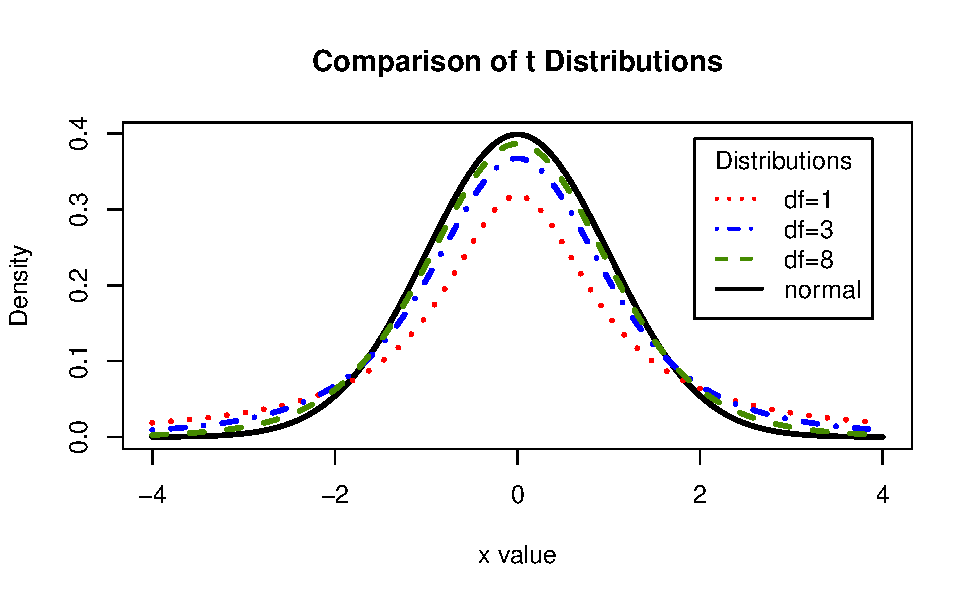
\includegraphics[width=0.7\linewidth]{11-A16-paired-theory_files/figure-latex/tdist-1} 

}

\caption{Comparison of the standard Normal vs t-distribution with various degrees of freedom}\label{fig:tdist}
\end{figure}

Like we saw in Chapter 5, we will not know the values of the parameters and must use the sample data to estimate them. Unlike with proportions, in which we only needed to estimate the population proportion, \(\pi\), quantitative sample data must be used to estimate both a population mean \(\mu\) and a population standard deviation \(\sigma\). This additional uncertainty will require us to use a theoretical distribution that is just a bit wider than the Normal distribution. Enter the \textbf{\(t\)-distribution}!

As you can seen from Figure \ref{fig:tdist}, the \(t\)-distributions (dashed and dotted lines) are centered at 0 just like a standard Normal distribution (solid line), but are slightly wider. The variability of a \(t\)-distribution depends on its degrees of freedom, which is calculated from the sample size of a study. (For a single sample of \(n\) observations or paired differences, the degrees of freedom is equal to \(n-1\).) Recall from previous classes that larger sample sizes tend to result in narrower sampling distributions. We see that here as well. The larger the sample size, the larger the degrees of freedom, the narrower the \(t\)-distribution. (In fact, a \(t\)-distribution with infinite degrees of freedom actually IS the standard Normal distribution!)

\hypertarget{summarize-and-visualize-the-data-3}{%
\subsubsection*{Summarize and visualize the data}\label{summarize-and-visualize-the-data-3}}
\addcontentsline{toc}{subsubsection}{Summarize and visualize the data}

Since the original data from the study are not available, we simulated data to match the means and standard deviations reported in the article. We will use these simulated data in the analysis below.

The following code plots each subject's time to read the colored words (above) and time to read the black words (below) connected by a grey line, a histogram of the differences in time to read words between the two conditions, and a boxplot displaying the pairwise differences in time (color \(-\) black).

\begin{Shaded}
\begin{Highlighting}[]
\NormalTok{color }\OtherTok{\textless{}{-}} \FunctionTok{read.csv}\NormalTok{(}\StringTok{"https://math.montana.edu/courses/s216/data/interference.csv"}\NormalTok{)}
\FunctionTok{paired\_observed\_plot}\NormalTok{(color)}

\NormalTok{color\_diff }\OtherTok{\textless{}{-}}\NormalTok{ color }\SpecialCharTok{\%\textgreater{}\%} 
  \FunctionTok{mutate}\NormalTok{(}\AttributeTok{differences =}\NormalTok{ DiffCol}\SpecialCharTok{{-}}\NormalTok{Black)}
\NormalTok{color\_diff }\SpecialCharTok{\%\textgreater{}\%}
  \FunctionTok{ggplot}\NormalTok{(}\FunctionTok{aes}\NormalTok{(}\AttributeTok{x =}\NormalTok{ differences))}\SpecialCharTok{+}
  \FunctionTok{geom\_boxplot}\NormalTok{()}\SpecialCharTok{+}
  \FunctionTok{labs}\NormalTok{(}\AttributeTok{title=}\StringTok{"Boxplot of the pairwise differences"}\NormalTok{,}
       \AttributeTok{x =} \StringTok{"Differences in time to read words (Color {-} Black)"}\NormalTok{)}
\end{Highlighting}
\end{Shaded}

\begin{center}\includegraphics[width=0.7\linewidth]{11-A16-paired-theory_files/figure-latex/unnamed-chunk-1-1} 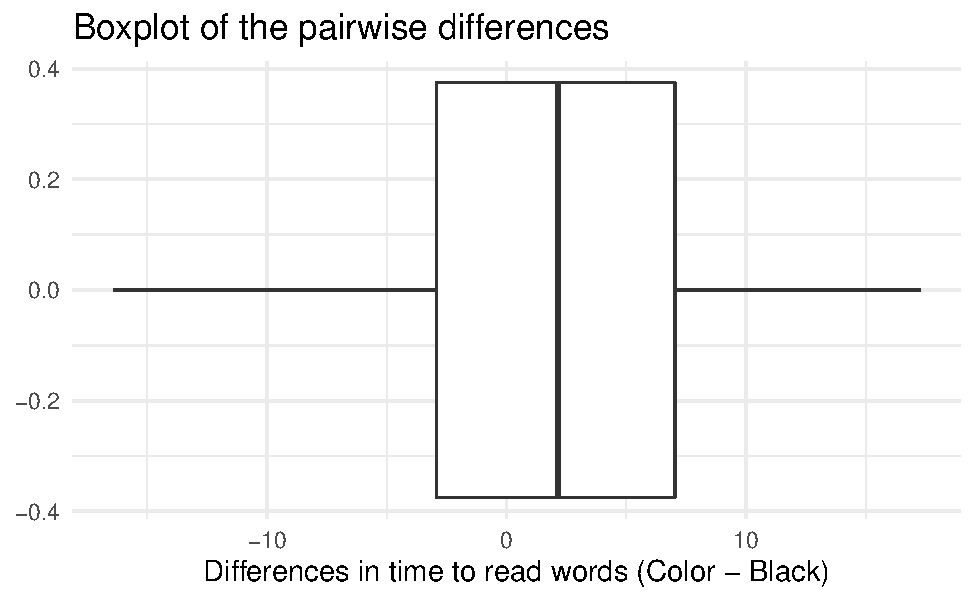
\includegraphics[width=0.7\linewidth]{11-A16-paired-theory_files/figure-latex/unnamed-chunk-1-2} \end{center}

The following code gives the summary statistics for the pairwise differences.

\begin{Shaded}
\begin{Highlighting}[]
\NormalTok{color\_diff }\SpecialCharTok{\%\textgreater{}\%} 
  \FunctionTok{summarise}\NormalTok{(}\FunctionTok{favstats}\NormalTok{(differences))}
\CommentTok{\#\textgreater{}      min     Q1 median     Q3   max mean       sd  n missing}
\CommentTok{\#\textgreater{} 1 {-}16.42 {-}2.925   2.15 7.0325 17.27  2.3 7.810196 70       0}
\end{Highlighting}
\end{Shaded}

\hypertarget{check-theoretical-conditions}{%
\subsubsection*{Check theoretical conditions}\label{check-theoretical-conditions}}
\addcontentsline{toc}{subsubsection}{Check theoretical conditions}

\begin{enumerate}
\def\labelenumi{\arabic{enumi}.}
\setcounter{enumi}{4}
\item
  How do you know the independence condition is met for these data?
  \vspace{0.8in}
\item
  Is the normality condition met to use the theory-based methods for analysis? Explain your answer.
  \vspace{1in}
\end{enumerate}

\hypertarget{use-statistical-inferential-methods-to-draw-inferences-from-the-data-1}{%
\subsubsection*{Use statistical inferential methods to draw inferences from the data}\label{use-statistical-inferential-methods-to-draw-inferences-from-the-data-1}}
\addcontentsline{toc}{subsubsection}{Use statistical inferential methods to draw inferences from the data}

To find the standardized statistic for the paired differences we will use the following formula:

\[T = \frac{\bar{x}_d - \mu_0}{SE(\bar{x}_d)},\]
where the standard error of the sample mean difference is:

\[SE(\bar{x}_d)=\frac{s_d}{\sqrt{n}}.\]

\begin{enumerate}
\def\labelenumi{\arabic{enumi}.}
\setcounter{enumi}{6}
\tightlist
\item
  Calculate the standard error of the sample mean difference.
\end{enumerate}

\vspace{0.5in}

\begin{enumerate}
\def\labelenumi{\arabic{enumi}.}
\setcounter{enumi}{7}
\tightlist
\item
  How many standard errors is the observed mean difference from the null mean difference?
\end{enumerate}

\vspace{0.5in}

Using the provided R script file, enter the T-score (for \texttt{xx}) into the \texttt{pt()} function. For single sample or paired data, degrees of freedom are found by subtracting 1 from the sample size. You should therefore use \texttt{df} = \(n_d-1 = 70 - 1 = 69\) and \texttt{lower.tail\ =\ FALSE} to find the p-value. Highlight and run line 23.

\begin{Shaded}
\begin{Highlighting}[]
\FunctionTok{pt}\NormalTok{(xx, }\AttributeTok{df=}\DecValTok{69}\NormalTok{, }\AttributeTok{lower.tail=}\ConstantTok{FALSE}\NormalTok{)}
\end{Highlighting}
\end{Shaded}

\begin{enumerate}
\def\labelenumi{\arabic{enumi}.}
\setcounter{enumi}{8}
\item
  Explain why we found the area above the T-score using \texttt{lower.tail\ =\ FALSE} in the code above.
  \vspace{0.3in}
\item
  What does this p-value mean, in the context of the study? Hint: it is the probability of what\ldots assuming what?
  \vspace{0.8in}
\end{enumerate}

\newpage

To calculate a theory-based confidence interval for the paired mean difference, use the following formula:

\[\bar{x}_d\pm t^* SE(\bar{x}_d).\]
We will need to find the \(t^*\) multiplier using the function \texttt{qt()}. The code below will return the 95th percentile of the \(t\) distribution with \texttt{df} = \(n_d - 1 = 70 - 1 = 69\).

\begin{Shaded}
\begin{Highlighting}[]
\FunctionTok{qt}\NormalTok{(}\FloatTok{0.95}\NormalTok{, }\AttributeTok{df =} \DecValTok{69}\NormalTok{, }\AttributeTok{lower.tail=}\ConstantTok{TRUE}\NormalTok{)}
\CommentTok{\#\textgreater{} [1] 1.667239}
\end{Highlighting}
\end{Shaded}

\begin{figure}

{\centering 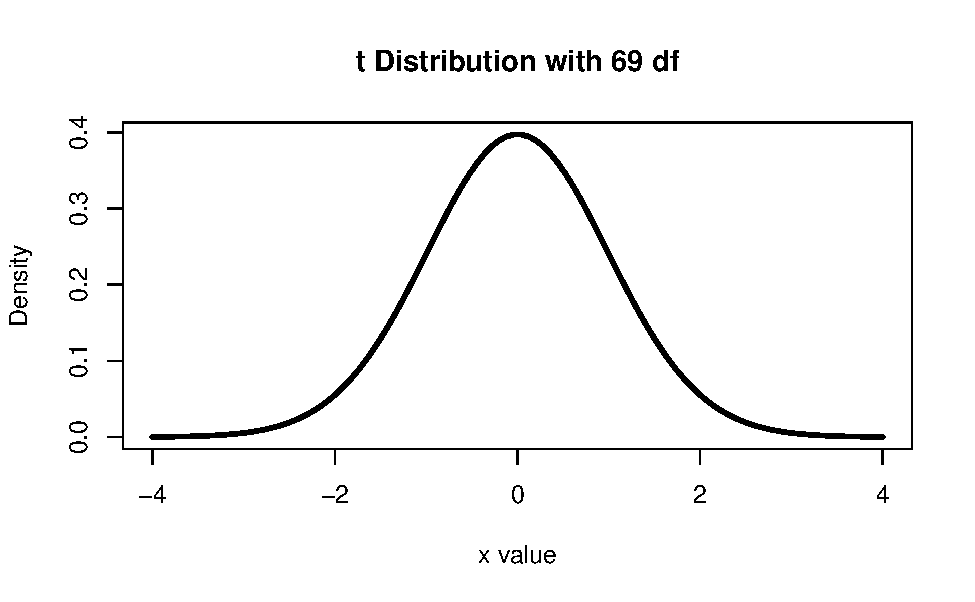
\includegraphics[width=0.7\linewidth]{11-A16-paired-theory_files/figure-latex/tstar-1} 

}

\caption{t-distribution with 69 degrees of freedom}\label{fig:tstar}
\end{figure}

\begin{enumerate}
\def\labelenumi{\arabic{enumi}.}
\setcounter{enumi}{10}
\item
  In Figure \ref{fig:tstar}, you see a t-distribution with 69 degrees of freedom. Label \(t^\star\) and \(-t^\star\) on that distribution. Write on the plot the percent of the \(t_{69}\)-distribution that is below \(-t^\star\), between \(-t^\star\) and \(t^\star\), and above \(t^\star\). Then use your plot to determine the confidence level associated with the \(t^\star\) value obtained.
  \vspace{0.3in}
\item
  Calculate the margin of error for the true paired mean difference using theory-based methods.
\end{enumerate}

\vspace{0.6in}

\begin{enumerate}
\def\labelenumi{\arabic{enumi}.}
\setcounter{enumi}{12}
\tightlist
\item
  Calculate the confidence interval for the true paired mean difference using theory-based methods.
\end{enumerate}

\newpage

\begin{enumerate}
\def\labelenumi{\arabic{enumi}.}
\setcounter{enumi}{13}
\tightlist
\item
  Interpret the confidence interval in context of the study.
\end{enumerate}

\vspace{1in}

\begin{enumerate}
\def\labelenumi{\arabic{enumi}.}
\setcounter{enumi}{14}
\tightlist
\item
  Do the results of the CI agree with the p-value? Explain your answer.
\end{enumerate}

\vspace{0.5in}

\begin{enumerate}
\def\labelenumi{\arabic{enumi}.}
\setcounter{enumi}{15}
\item
  Write a conclusion to the test in context of the study.
  \vspace{0.6in}
\item
  The abstract states, that the conflicting color stimuli ``caused an increase of 2.3 seconds or 5.6\% over the normal time for reading the same words printed in black.'' Is this statement valid? Explain.
  \vspace{0.6in}
\end{enumerate}

\hypertarget{take-home-messages-18}{%
\subsection{Take-home messages}\label{take-home-messages-18}}

\begin{enumerate}
\def\labelenumi{\arabic{enumi}.}
\item
  In order to use theory-based methods for dependent groups (paired data), the independent observational units and normality conditions must be met.
\item
  A T-score is compared to a \(t\)-distribution with \(n - 1\) df in order to calculate a one-sided p-value. To find a two-sided p-value using theory-based methods we need to multiply the one-sided p-value by 2.
\item
  A \(t^*\) multiplier is found by obtaining the bounds of the middle X\% (X being the desired confidence level) of a \(t\)-distribution with \(n - 1\) df.
\end{enumerate}

\hypertarget{additional-notes-17}{%
\subsection{Additional notes}\label{additional-notes-17}}

Use this space to summarize your thoughts and take additional notes on today's activity and material covered

\newpage

\hypertarget{week-11-lab-swearing}{%
\section{Week 11 Lab: Swearing}\label{week-11-lab-swearing}}

\setstretch{1}

\hypertarget{learning-outcomes-22}{%
\subsection{Learning outcomes}\label{learning-outcomes-22}}

\begin{itemize}
\item
  Identify whether a study is a paired design or independent groups
\item
  Given a research question involving paired data, construct the null and alternative hypotheses
  in words and using appropriate statistical symbols.
\item
  Describe and perform a simulation-based hypothesis test for a mean difference.
\item
  Interpret and evaluate a p-value for a hypothesis test for a mean difference.
\item
  Use bootstrapping methods to find a confidence interval for a mean difference.
\item
  Interpret a confidence interval for a mean difference.
\end{itemize}

\hypertarget{type-of-samples}{%
\subsection{Type of samples}\label{type-of-samples}}

For each of the following scenarios, determine whether the samples are paired or independent.

\begin{enumerate}
\def\labelenumi{\arabic{enumi}.}
\item
  Researchers interested in studying the effect of a medical treatment on insulin rate measured insulin rates of 30 patients before and after the medical treatment.
  \vspace{0.3in}
\item
  \textbf{A university is planning to bring emotional support animals to campus during finals week and wants to determine which type of animals are more effective at calming students. Anxiety levels will be measured before and after each student interacts with either a dog or a cat. The university will then compare change in anxiety levels between the `dog' people and the `cat' people.}
  \vspace{0.3in}
\item
  An industry leader is investigating a possible wage gap between male and non-male employees. Twenty companies within the industry are randomly selected and the average salary for all males and non-males in mid-management positions is recorded for each company.
  \vspace{0.3in}
\end{enumerate}

\hypertarget{swearing}{%
\subsection{Swearing}\label{swearing}}

Profanity (language considered obscene or taboo) and society's attitude about its acceptableness is a highly debated topic, but does swearing serve a physiological purpose or function? Previous research has shown that swearing produces increased heart rates and higher levels of skin conductivity. It is theorized that since swearing provokes intense emotional responses, it acts as a distracter, allowing a person to withstand higher levels of pain. To explore the relationship between swearing and increased pain tolerance, researchers from Keele University (Staffordshire, UK) recruited 83 native English-speaking participants (Stephens and Robertson 2020). Each volunteer performed two trials holding a hand in an ice-water bath, once while repeating the ``f-word'' every three seconds, and once while repeating a neutral word (``table''). The order of the word to repeat was randomly assigned. Researchers recorded the length of time, in seconds, from the moment the participant indicated they were in pain until they removed their hand from the ice water for each trial. They hope to find evidence that pain tolerance is greater (longer times) when a person swears compared to when they say a neutral word, on average. Use Swear -- Neutral as the order of subtraction.

\begin{enumerate}
\def\labelenumi{\arabic{enumi}.}
\setcounter{enumi}{3}
\tightlist
\item
  What does \(\mu_d\) represent in the context of this study?
\end{enumerate}

\vspace{0.8in}

\begin{enumerate}
\def\labelenumi{\arabic{enumi}.}
\setcounter{enumi}{4}
\tightlist
\item
  Write out the null hypothesis in proper notation for this study.
\end{enumerate}

\vspace{0.8in}

\begin{enumerate}
\def\labelenumi{\arabic{enumi}.}
\setcounter{enumi}{5}
\tightlist
\item
  What sign (\(<\), \(>\), or \(\neq\)) would you use in the alternative hypothesis for this study? Explain your choice.
\end{enumerate}

\vspace{0.5in}

Upload and open the R script file for Week 11 lab. Upload and import the csv file, \texttt{pain\_tolerance}. Enter the name of the data set (see the environment tab) for datasetname in the R script file in line 6. Highlight and run lines 1--7 to load the data and create a paired plot of the data.

\begin{Shaded}
\begin{Highlighting}[]
\NormalTok{swearing }\OtherTok{\textless{}{-}}\NormalTok{ datasetname}
\FunctionTok{paired\_observed\_plot}\NormalTok{(swearing)}
\end{Highlighting}
\end{Shaded}

\begin{enumerate}
\def\labelenumi{\arabic{enumi}.}
\setcounter{enumi}{6}
\tightlist
\item
  Based on the plots, does there appear to be some evidence in favor of the alternative hypothesis? How do you know?
  \vspace{0.4in}
\end{enumerate}

Enter the outcome for group 1 (\texttt{Swear}) for \texttt{measurement\_1} and the outcome for group 2 (\texttt{Neutral}) for \texttt{measurement\_2} in line 10. Highlight and run lines 9--12 to get the summary statistics for the data.

\begin{Shaded}
\begin{Highlighting}[]
\NormalTok{swearing\_diff }\OtherTok{\textless{}{-}}\NormalTok{ swearing }\SpecialCharTok{\%\textgreater{}\%} 
  \FunctionTok{mutate}\NormalTok{(}\AttributeTok{differences =}\NormalTok{ measurement\_1 }\SpecialCharTok{{-}}\NormalTok{ measurement\_2)}
\NormalTok{swearing\_diff }\SpecialCharTok{\%\textgreater{}\%} 
    \FunctionTok{summarise}\NormalTok{(}\FunctionTok{favstats}\NormalTok{(differences))}
\end{Highlighting}
\end{Shaded}

\begin{enumerate}
\def\labelenumi{\arabic{enumi}.}
\setcounter{enumi}{7}
\item
  What is the value of \(\bar{x}_d\)? What is the sample size?
  \vspace{0.25in}
\item
  \textbf{How far, on average, is each difference in pain tolerance from the mean of the differences in pain tolerance? What is the appropriate notation for this value?}
\end{enumerate}

\vspace{0.5in}

\hypertarget{use-statistical-inferential-methods-to-draw-inferences-from-the-data-2}{%
\subsection*{Use statistical inferential methods to draw inferences from the data}\label{use-statistical-inferential-methods-to-draw-inferences-from-the-data-2}}
\addcontentsline{toc}{subsection}{Use statistical inferential methods to draw inferences from the data}

\begin{enumerate}
\def\labelenumi{\arabic{enumi}.}
\setcounter{enumi}{9}
\tightlist
\item
  Using the provided graphs and summary statistics, determine if both theory-based methods and simulation methods could be used to analyze the data. Explain your reasoning.
\end{enumerate}

\vspace{0.8in}

\hypertarget{hypothesis-test-1}{%
\subsection*{Hypothesis test}\label{hypothesis-test-1}}
\addcontentsline{toc}{subsection}{Hypothesis test}

Remember that the null distribution is created based on the assumption the null hypothesis is true. In this study, the null hypothesis states that swearing does not affect pain tolerance, or that the length of time a subject kept their hand in the water would be the same whether the patient was swearing or not.

We will use the \texttt{paired\_test()} function in R (in the \texttt{catstats} package) to simulate the null distribution of sample mean differences and compute a p-value.

\begin{enumerate}
\def\labelenumi{\arabic{enumi}.}
\setcounter{enumi}{10}
\tightlist
\item
  When using the \texttt{paired\_test()} function, we need to enter the name of the data set, either the order of subtraction (if the data set has both measurements) or the name of the differences (if the data set contains them). We will also need to provide R with the observed mean difference, the direction of the alternative hypothesis, and the shift required in order to force the null hypothesis to be true. The name of the data set as shown above is \texttt{swearing\_diff} and the column of differences is called \texttt{differences}. What values should be entered for each of the following to create 1000 simulated samples?
\end{enumerate}

\vspace{1mm}

\begin{itemize}
\tightlist
\item
  shift:
\end{itemize}

\vspace{.2in}

\begin{itemize}
\tightlist
\item
  As extreme as:
\end{itemize}

\vspace{.2in}

\begin{itemize}
\tightlist
\item
  Direction (\texttt{"greater"}, \texttt{"less"}, or \texttt{"two-sided"}):
\end{itemize}

\vspace{.2in}

\begin{itemize}
\tightlist
\item
  Number of repetitions:
\end{itemize}

\vspace{.2in}

\begin{enumerate}
\def\labelenumi{\arabic{enumi}.}
\setcounter{enumi}{11}
\tightlist
\item
  Simulate a null distribution and compute the p-value. Using the R script file for this lab, enter your answers for question 11 in place of the \texttt{xx}'s to produce the null distribution with 1000 simulations. Highlight and run lines 15--21.
\end{enumerate}

\begin{Shaded}
\begin{Highlighting}[]
\FunctionTok{paired\_test}\NormalTok{(}\AttributeTok{data =}\NormalTok{ swearing}\SpecialCharTok{$}\NormalTok{differences,   }\CommentTok{\# Vector of differences }
                                 \CommentTok{\# or data set with column for each group}
        \AttributeTok{shift =}\NormalTok{ xx,   }\CommentTok{\# Shift needed for bootstrap hypothesis test}
        \AttributeTok{as\_extreme\_as =}\NormalTok{ xx,  }\CommentTok{\# Observed statistic}
        \AttributeTok{direction =} \StringTok{"xx"}\NormalTok{,  }\CommentTok{\# Direction of alternative}
        \AttributeTok{number\_repetitions =}\NormalTok{ xx,  }\CommentTok{\# Number of simulated samples for null distribution}
        \AttributeTok{which\_first =} \DecValTok{1}\NormalTok{)  }\CommentTok{\# Not needed when using calculated differences}
\end{Highlighting}
\end{Shaded}

~~~~~~~Sketch the null distribution created using the \texttt{paired\_test} code.

\vspace{1.5in}

\hypertarget{communicate-the-results-and-answer-the-research-question-3}{%
\subsection*{Communicate the results and answer the research question}\label{communicate-the-results-and-answer-the-research-question-3}}
\addcontentsline{toc}{subsection}{Communicate the results and answer the research question}

\begin{enumerate}
\def\labelenumi{\arabic{enumi}.}
\setcounter{enumi}{12}
\tightlist
\item
  \textbf{Report the p-value. Based off of this p-value and a 1\% significance level, what decision would you make about the null hypothesis? What potential error might you be making based on that decision?}
\end{enumerate}

\vspace{0.5in}

\begin{enumerate}
\def\labelenumi{\arabic{enumi}.}
\setcounter{enumi}{13}
\tightlist
\item
  Do you expect the 98\% confidence interval to contain the null value of zero? Explain.
\end{enumerate}

\vspace{0.8in}

\hypertarget{confidence-interval-1}{%
\subsection*{Confidence interval}\label{confidence-interval-1}}
\addcontentsline{toc}{subsection}{Confidence interval}

We will use the \texttt{paired\_bootstrap\_CI()} function in R (in the \texttt{catstats} package) to simulate the bootstrap distribution of sample mean differences and calculate a confidence interval.

\begin{enumerate}
\def\labelenumi{\arabic{enumi}.}
\setcounter{enumi}{14}
\tightlist
\item
  Using bootstrapping and the provided R script file, find a 98\% confidence interval. Fill in the missing values/numbers in the \texttt{paired\_bootstrap\_CI()} function to create the 98\% confidence interval. Highlight and run lines 24--27. \textbf{Upload a copy of the bootstrap distribution created to Gradescope for your group.}
\end{enumerate}

\begin{Shaded}
\begin{Highlighting}[]
\FunctionTok{paired\_bootstrap\_CI}\NormalTok{(}\AttributeTok{data =}\NormalTok{ swearing\_diff}\SpecialCharTok{$}\NormalTok{differences, }\CommentTok{\# Enter vector of differences}
                    \AttributeTok{number\_repetitions =} \DecValTok{1000}\NormalTok{, }\CommentTok{\# Number of bootstrap samples for CI}
                    \AttributeTok{confidence\_level =}\NormalTok{ xx,  }\CommentTok{\# Confidence level in decimal form}
                    \AttributeTok{which\_first =} \DecValTok{1}\NormalTok{)  }\CommentTok{\# Not needed when entering vector of differences}
\end{Highlighting}
\end{Shaded}

\newpage

~~~~~~~Sketch the bootstrap distribution created using the code. Report the 98\% confidence interval in interval notation.

\vspace{1.5in}

\begin{enumerate}
\def\labelenumi{\arabic{enumi}.}
\setcounter{enumi}{15}
\tightlist
\item
  Interpret the \emph{confidence level} of the interval you calculated in question 15.
\end{enumerate}

\vspace{0.8in}

\begin{enumerate}
\def\labelenumi{\arabic{enumi}.}
\setcounter{enumi}{16}
\tightlist
\item
  Write a paragraph summarizing the results of this study as if you were describing the results to your roommate. \textbf{Upload a copy of your group's paragraph to Gradescope.} Be sure to describe:
\end{enumerate}

\begin{itemize}
\item
  Summary statistic
\item
  P-value and interpretation
\item
  Conclusion (written to answer the research question)
\item
  Confidence interval and interpretation
\item
  Scope of inference
\end{itemize}

\vspace{2.6in}

\newpage

\hypertarget{inference-for-a-quantitative-response-with-independent-samples}{%
\chapter{Inference for a Quantitative Response with Independent Samples}\label{inference-for-a-quantitative-response-with-independent-samples}}

\hypertarget{week-12-reading-guide-inference-for-a-difference-in-two-means}{%
\section{Week 12 Reading Guide: Inference for a Difference in Two Means}\label{week-12-reading-guide-inference-for-a-difference-in-two-means}}

\hypertarget{chapter-19-inference-for-comparing-two-independent-means}{%
\subsection*{Chapter 19 (Inference for comparing two independent means)}\label{chapter-19-inference-for-comparing-two-independent-means}}
\addcontentsline{toc}{subsection}{Chapter 19 (Inference for comparing two independent means)}

\textbf{Videos}

\begin{itemize}
\tightlist
\item
  19.1
\item
  19.2
\item
  19.3Tests
\item
  19.3Intervals
\end{itemize}

\setstretch{1.25}

\hypertarget{reminders-from-previous-sections-10}{%
\subsubsection*{Reminders from previous sections}\label{reminders-from-previous-sections-10}}
\addcontentsline{toc}{subsubsection}{Reminders from previous sections}

\(n_1\)= sample size of group 1

\(n_2\) = sample size of group 2

\(\overline{x}\) = sample mean

\(s\) = sample standard deviation

\(\mu\) = population mean

\(\sigma\) = population standard deviation

General steps of a hypothesis test:

\begin{enumerate}
\def\labelenumi{\arabic{enumi}.}
\item
  Frame the research question in terms of hypotheses.
\item
  Collect and summarize data using a test statistic.
\item
  Assume the null hypothesis is true, and simulate or mathematically model a null distribution for the test statistic.
\item
  Compare the observed test statistic to the null distribution to calculate a p-value.
\item
  Make a conclusion based on the p-value and write the conclusion in context.
\end{enumerate}

Parameter: a value summarizing a variable(s) for a population.

Statistic: a value summarizing a variable(s) for a sample.

Sampling distribution: plot of statistics from 1000s of samples of the same size taken from the same population.

Standard deviation of a statistic: the variability of statistics from 1000s of samples; how far, on average, each statistic is from the true value of the parameter.

Standard error of a statistic: estimated standard deviation of a statistic.

Hypothesis test: a process to determine how strong the evidence of an effect is. Also called a `significance test'.

Simulation-based method: Simulate lots of samples of size \(n\) under assumption of the null hypothesis, then find the proportion of the simulations that are at least as extreme as the observed sample statistic.

Theory-based method: Develop a mathematical model for the sampling distribution of the statistic under the null hypothesis and use the model to calculate the probability of the observed sample statistic (or one more extreme) occurring.

Null hypothesis (\(H_0\)): the skeptical perspective; no difference; no change; no effect; random chance; what the researcher hopes to prove is \textbf{wrong}.

Alternative hypothesis (\(H_A\)): the new perspective; a difference/increase/decrease; an effect; not random chance; what the researcher hopes to prove is \textbf{correct}.

Null value: the value of the parameter when we assume the null hypothesis is true (labeled as \(parameter_0\)).

Null distribution: the simulated or modeled distribution of statistics (sampling distribution) we would expect to occur if the null hypothesis is true.

P-value: probability of seeing the observed sample data, or something more extreme, assuming the null hypothesis is true.

\(\implies\) Lower the p-value the stronger the evidence AGAINST the null hypothesis and FOR the alternative hypothesis.

Decision: a determination of whether to reject or fail to reject a null hypothesis based on a p-value and a pre-set level of significance.

\begin{itemize}
\item
  If p-value \(\leq \alpha\), then reject \(H_0\).
\item
  If p-value \(> \alpha\), then fail to reject \(H_0\).
\end{itemize}

Significance level (\(\alpha\)): a threshold used to determine if a p-value provides enough evidence to reject the null hypothesis or not.

\rgi Common levels of \(\alpha\) include 0.01, 0.05, and 0.10.

Statistically significant: results are considered statistically significant if the p-value is below the significance level.

Confidence interval: a process to determine how large an effect is; a range of plausible values for the parameter. Also called `estimation'.

Margin of error: the value that is added to and subtracted from the sample statistic to create a confidence interval; half the width of a confidence interval.

Bootstrapping: the process of drawing with replacement \(n\) times from the original sample.

Bootstrapped resample: a random sample of size \(n\) from the original sample, selected with replacement.

Bootstrapped statistic: the statistic recorded from the bootstrapped resample.

Confidence level: how confident we are that the confidence interval will capture the parameter.

Bootstrap \(X\)\% confidence interval: (\((\frac{(1-X)}{2})^{th}\) percentile, \((X+(\frac{(1-X)}{2})^{th}\) percentile) of a bootstrap distribution.

Central Limit Theorem: For large sample sizes, the sampling distribution of a sample mean (or proportion) will be approximately normal (bell-shaped and symmetric).

\(t\)-distribution: A bell-shaped symmetric distribution, centered at 0, wider than the standard normal distribution.

\begin{itemize}
\tightlist
\item
  The variability in a \(t\)-distribution depends on the sample size (used to calculate degrees of freedom --- df for short).
\item
  The \(t\)-distribution gets closer to the standard normal distribution as df increases.
\end{itemize}

Degrees of freedom (df): describes the variability of the \(t\)-distribution.

T-score: the name for a standardized statistic which is compared to a \(t\)-distribution.

\hypertarget{notes-24}{%
\subsubsection*{Notes}\label{notes-24}}
\addcontentsline{toc}{subsubsection}{Notes}

To create a \textbf{simulated null distribution} of differences in independent sample means,

\rgi How many cards will you need and how will the cards be labeled?
\rgs

\rgi What do you do with the cards after labeling them?
\rgs

\rgi After shuffling, what value will be plotted on the simulated null distribution?
\rgs

To create a \textbf{bootstrap distribution} of differences in independent sample means,

\rgi How many cards will you need and how will the cards be labeled?
\rgs

\rgi What do you do with the cards after labeling them?
\rgs

\rgi After shuffling, what value will be plotted on the bootstrap distribution?
\rgs

Conditions to use the CLT for a difference in independent sample means:

\rgi Independence:
\rgs

\rgi \rgi Checked by:
\rgs

\rgi Normality:
\rgs

\rgi \rgi Checked by:
\rgs

In a two-sample \(t\)-test, how are the degrees of freedom determined?
\rgs        

True or false: A large p-value indicates that the null hypothesis is true.
\rgs

\hypertarget{formulas-5}{%
\subsubsection*{Formulas}\label{formulas-5}}
\addcontentsline{toc}{subsubsection}{Formulas}

\(SE(\overline{x_1} - \overline{x_2})=\)
\rgs

\(T=\)
\rgs

Confidence interval for a difference in independent sample means:
\rgs

\hypertarget{notation-4}{%
\subsubsection*{Notation}\label{notation-4}}
\addcontentsline{toc}{subsubsection}{Notation}

\(\mu_1\) represents
\rgs

\(\mu_2\) represents
\rgs

\(\sigma_1\) represents
\rgs

\(\sigma_2\) represents
\rgs

\(\overline{x_1}\) represents
\rgs

\(\overline{x_2}\) represents
\rgs

\(s_1\) represents
\rgs

\(s_2\) represents
\rgs

\hypertarget{example-from-section-19.1-test-scores}{%
\subsubsection*{Example from section 19.1: Test scores}\label{example-from-section-19.1-test-scores}}
\addcontentsline{toc}{subsubsection}{Example from section 19.1: Test scores}

\begin{enumerate}
\def\labelenumi{\arabic{enumi}.}
\item
  What are the observational units?
  \rgs
\item
  What are the sample statistics presented in this example? What notation would be used to represent each value?
  \rgs
\item
  What is the parameter representing in the context of this problem? What notation would be used to represent this parameter?
  \rgs
  \rgs
\item
  What is the research question?
  \rgs
\item
  Write the null and alternative hypothesis in appropriate notation.
  \rgs
\item
  How could we use cards to simulate \textbf{one} sample \emph{which assumes the null hypothesis is true}? How many cards? What is written on the cards? What would we do with the cards? What would you record once you have a simulated sample?
  \rgs
  \rgs
  \rgs
\item
  After 1000 shuffles are generated, where is the resulting simulated distribution centered? Why does that make sense?
  \rgs
  \rgs
\item
  How was the p-value for this test found? The proportion of simulated null samples at \_\_\_\_ or \_\_\_\_\_\_\_\_\_\_\_.
  \rgs
\item
  Interpret the p-value in the context of the problem.
  \rgs
  \rgs
\item
  From these data, can we conclude the exams are equally difficult?
  \rgs
\item
  What type of error may have occurred at the 5\% significance level? Interpret that error in context.
  \rgs
  \rgs
\end{enumerate}

\hypertarget{example-from-section-19.2-esc-and-heart-attacks}{%
\subsubsection*{Example from section 19.2: ESC and heart attacks}\label{example-from-section-19.2-esc-and-heart-attacks}}
\addcontentsline{toc}{subsubsection}{Example from section 19.2: ESC and heart attacks}

\begin{enumerate}
\def\labelenumi{\arabic{enumi}.}
\item
  What is the research question?
  \rgs
\item
  What are the observational units?
  \rgs
\item
  What variables are recorded? Give the type (categorical or quantitative) and role (explanatory or response) of each.
  \rgs
  \rgs
\item
  What are the sample statistics presented in this example? What notation would be used to represent each value?
  \rgs
\item
  What is the parameter representing in the context of this problem? What notation would be used to represent this parameter?
  \rgs
  \rgs
\item
  How could we use cards to simulate \textbf{one} bootstrap resample \emph{which does not assume the null hypothesis is true}? How many cards? What is written on the cards? What would we do with the cards? What would you record once you have a simulated sample?
  \rgs
  \rgs
  \rgs
\item
  After 1000 resamples are generated, where is the resulting bootstrap distribution centered? Why does that make sense?
  \rgs
  \rgs
\item
  Does the 90\% confidence interval provide evidence of a difference across the two treatments?
  \rgs
  \rgs
\end{enumerate}

\hypertarget{example-from-section-19.3-north-carolina-births}{%
\subsubsection*{Example from section 19.3: North Carolina births}\label{example-from-section-19.3-north-carolina-births}}
\addcontentsline{toc}{subsubsection}{Example from section 19.3: North Carolina births}

\begin{enumerate}
\def\labelenumi{\arabic{enumi}.}
\item
  What is the research question?
  \rgs
\item
  What are the observational units?
  \rgs
\item
  What variables will be analyzed? Give the type and role of each.
  \rgs
  \rgs
\item
  Can the results of this study be generalized to a larger population?
  \rgs
\item
  Are causal conclusions appropriate for these data?
  \rgs
\item
  Write the null and the alternative hypotheses in words.
  \rgs
  \rgs
\item
  Write the null and the alternative hypotheses in notation.
  \rgs
\item
  What are the sample statistics presented in this example? What notation would be used to represent each value?
  \rgs
\item
  Are the independence and normality conditions satisfied?
  \rgs
  \rgs
\item
  Calculate the standard error of the difference in sample means.
  \rgs
  \rgs
\item
  Calculate the T-score (the standardized statistic for the sample mean).
  \rgs
  \rgs
\item
  What distribution should the T-score be compared to in order to calculate a p-value?
  \rgs
\item
  What was the p-value of the test?
  \rgs
\item
  What conclusion should the researcher make?
  \rgs
  \rgs
\item
  Calculate a 95\% confidence interval for the parameter of interest using \texttt{qt(0.975,\ df\ =\ 49)\ =\ 1.677} as the \(t^\star\) value.
  \rgs
  \rgs
\item
  Interpret your interval in the context of the problem.
  \rgs
  \rgs
\end{enumerate}

\newpage

\hypertarget{activity-12-does-behavior-impact-performance}{%
\section{Activity 12: Does behavior impact performance?}\label{activity-12-does-behavior-impact-performance}}

\setstretch{1}

\hypertarget{learning-outcomes-23}{%
\subsection{Learning outcomes}\label{learning-outcomes-23}}

\begin{itemize}
\item
  Given a research question involving one categorical explanatory variable and one quantitative response variable, construct the null and alternative hypotheses
  in words and using appropriate statistical symbols.
\item
  Describe and perform a simulation-based hypothesis test for a difference in means.
\item
  Interpret and evaluate a p-value for a simulation-based hypothesis test for a difference in means.
\item
  Use bootstrapping to find a confidence interval for a difference in means.
\item
  Interpret a confidence interval for a difference in means.
\item
  Use a confidence interval to determine the conclusion of a hypothesis test.
\end{itemize}

\hypertarget{terminology-review-19}{%
\subsection{Terminology review}\label{terminology-review-19}}

In today's activity, we will use simulation-based methods to analyze the association between one categorical explanatory variable and one quantitative response variable, where the groups formed by the categorical variable are independent. Some terms covered in this activity are:

\begin{itemize}
\item
  Independent groups
\item
  Difference in means
\end{itemize}

To review these concepts, see Chapter 19 in the textbook.

\hypertarget{behavior-and-performance}{%
\subsection{Behavior and Performance}\label{behavior-and-performance}}

A study in the Academy of Management Journal (Porath 2017) investigated how rude behaviors influence a victim's task performance. Randomly selected college students enrolled in a management course were randomly assigned to one of two experimental conditions: rudeness condition (45 students) and control group (53 students). Each student was asked to write down as many uses for a brick as possible in five minutes; this value (total number of uses) was used as a performance measure for each student, where higher values indicate better performance. During this time another individual showed up late for class. For those students in the rudeness condition, the facilitator displayed rudeness by berating the students in general for being irresponsible and unprofessional (due to the late-arriving person). No comments were made about the late-arriving person for students in the control group. Is there evidence that the average performance score for students in the rudeness condition is lower than for students in the control group? Use the order of subtraction of rudeness -- control.

\begin{Shaded}
\begin{Highlighting}[]
\CommentTok{\# Read in data set}
\NormalTok{rude }\OtherTok{\textless{}{-}} \FunctionTok{read.csv}\NormalTok{(}\StringTok{"https://math.montana.edu/courses/s216/data/rude.csv"}\NormalTok{)}
\end{Highlighting}
\end{Shaded}

\newpage

\begin{Shaded}
\begin{Highlighting}[]
\CommentTok{\# Side{-}by{-}side box plots}
\NormalTok{rude }\SpecialCharTok{\%\textgreater{}\%}
\FunctionTok{ggplot}\NormalTok{(}\FunctionTok{aes}\NormalTok{(}\AttributeTok{x =}\NormalTok{ condition, }\AttributeTok{y =}\NormalTok{ number\_of\_uses)) }\SpecialCharTok{+}
    \FunctionTok{geom\_boxplot}\NormalTok{() }\SpecialCharTok{+} 
    \FunctionTok{labs}\NormalTok{(}\AttributeTok{title =} \StringTok{"Number of Uses for a Brick based on Behavior Condition"}\NormalTok{,}
         \AttributeTok{x =} \StringTok{"Behavior"}\NormalTok{) }
\end{Highlighting}
\end{Shaded}

\begin{center}\includegraphics[width=0.6\linewidth]{12-A17-inference-1ofeach-simulation_files/figure-latex/unnamed-chunk-2-1} \end{center}

\begin{Shaded}
\begin{Highlighting}[]
\CommentTok{\# Summary statistics}
\NormalTok{rude }\SpecialCharTok{\%\textgreater{}\%} 
     \FunctionTok{summarize}\NormalTok{(}\FunctionTok{favstats}\NormalTok{(number\_of\_uses }\SpecialCharTok{\textasciitilde{}}\NormalTok{ condition))}
\end{Highlighting}
\end{Shaded}

\begin{verbatim}
#>   condition min Q1 median Q3 max      mean       sd  n missing
#> 1   control   0  6     12 17  30 11.811321 7.382559 53       0
#> 2  rudeness   0  6      9 11  18  8.511111 3.992164 45       0
\end{verbatim}

\hypertarget{quantitative-variables-review}{%
\subsubsection*{Quantitative variables review}\label{quantitative-variables-review}}
\addcontentsline{toc}{subsubsection}{Quantitative variables review}

\begin{enumerate}
\def\labelenumi{\arabic{enumi}.}
\tightlist
\item
  The two variables assessed in this study are behavior and number of uses for a brick. Identify the role for each variable (explanatory or response).
\end{enumerate}

\vspace{.4in}

\begin{enumerate}
\def\labelenumi{\arabic{enumi}.}
\setcounter{enumi}{1}
\tightlist
\item
  Which group (control or rudeness) has the highest center in the distributions of number of uses for a brick? Explain which measure of center you are using.
\end{enumerate}

\vspace{.4in}

\begin{enumerate}
\def\labelenumi{\arabic{enumi}.}
\setcounter{enumi}{2}
\tightlist
\item
  Using the side-by-side box plots, which group has the largest spread in number of uses for a brick? How did you make that choice?
\end{enumerate}

\vspace{.4in}

\newpage

\begin{enumerate}
\def\labelenumi{\arabic{enumi}.}
\setcounter{enumi}{3}
\tightlist
\item
  Is this an experiment or an observational study? Justify your answer.
\end{enumerate}

\vspace{1in}

\begin{enumerate}
\def\labelenumi{\arabic{enumi}.}
\setcounter{enumi}{4}
\tightlist
\item
  Is this a paired data set or two independent groups? Explain your reasoning.
\end{enumerate}

\vspace{1in}

\hypertarget{ask-a-research-question-4}{%
\subsubsection*{Ask a research question}\label{ask-a-research-question-4}}
\addcontentsline{toc}{subsubsection}{Ask a research question}

\begin{enumerate}
\def\labelenumi{\arabic{enumi}.}
\setcounter{enumi}{5}
\tightlist
\item
  Write out the parameter of interest in context of the study. Use proper notation and be sure to define your subscripts.
\end{enumerate}

\vspace{1in}

\begin{enumerate}
\def\labelenumi{\arabic{enumi}.}
\setcounter{enumi}{6}
\tightlist
\item
  Write out the null hypothesis in words.
\end{enumerate}

\vspace{1in}

\begin{enumerate}
\def\labelenumi{\arabic{enumi}.}
\setcounter{enumi}{7}
\tightlist
\item
  Write the alternative hypothesis in notation.
\end{enumerate}

\vspace{0.5in}

\hypertarget{summarize-and-visualize-the-data-4}{%
\subsubsection*{Summarize and visualize the data}\label{summarize-and-visualize-the-data-4}}
\addcontentsline{toc}{subsubsection}{Summarize and visualize the data}

\begin{enumerate}
\def\labelenumi{\arabic{enumi}.}
\setcounter{enumi}{8}
\tightlist
\item
  Calculate the summary statistic of interest (difference in means). What is the appropriate notation for this statistic?
\end{enumerate}

\vspace{0.5in}

\newpage

\hypertarget{use-statistical-inferential-methods-to-draw-inferences-from-the-data-3}{%
\subsubsection*{Use statistical inferential methods to draw inferences from the data}\label{use-statistical-inferential-methods-to-draw-inferences-from-the-data-3}}
\addcontentsline{toc}{subsubsection}{Use statistical inferential methods to draw inferences from the data}

\hypertarget{hypothesis-test-2}{%
\paragraph*{Hypothesis test}\label{hypothesis-test-2}}
\addcontentsline{toc}{paragraph}{Hypothesis test}

Remember that the null distribution is created based on the assumption the null hypothesis is true. In this study, the null hypothesis states that there is no association between the two variables. This means that the values observed in the data set would have been the same regardless of the behavior condition.

To demonstrate this simulation, we could create cards to simulate a sample.

\begin{enumerate}
\def\labelenumi{\arabic{enumi}.}
\setcounter{enumi}{9}
\tightlist
\item
  How many cards would we start with?
\end{enumerate}

\vspace{0.3in}

\begin{enumerate}
\def\labelenumi{\arabic{enumi}.}
\setcounter{enumi}{10}
\tightlist
\item
  What would we write on each card?
\end{enumerate}

\vspace{0.3in}

\begin{enumerate}
\def\labelenumi{\arabic{enumi}.}
\setcounter{enumi}{11}
\tightlist
\item
  Next, we would mix the cards together and shuffle into two piles. How many cards will go into each pile? What should we label the piles?
\end{enumerate}

\vspace{.8in}

\begin{enumerate}
\def\labelenumi{\arabic{enumi}.}
\setcounter{enumi}{12}
\tightlist
\item
  What value would be calculated from the cards and plotted on the null distribution? \emph{Hint}: What statistic are we calculating from the data?
\end{enumerate}

\vspace{0.3in}

\begin{enumerate}
\def\labelenumi{\arabic{enumi}.}
\setcounter{enumi}{13}
\tightlist
\item
  Would you expect your simulated statistic to be closer to the null value of zero than the difference in means calculated from the sample? Explain why this makes sense.
\end{enumerate}

\vspace{0.8in}

We will use the \texttt{two\_mean\_test()} function in R (in the \texttt{catstats} package) to simulate the null distribution of differences in sample means and compute a p-value.

\newpage

\begin{enumerate}
\def\labelenumi{\arabic{enumi}.}
\setcounter{enumi}{14}
\tightlist
\item
  When using the \texttt{two\_mean\_test()} function, we need to enter the name of the response variable, \texttt{number\_of\_uses}, and the name of the explanatory variable, \texttt{condition}, for the formula. The name of the data set as shown above is \texttt{rude}. What values should be entered for each of the following to create 1000 simulated samples?
\end{enumerate}

\begin{itemize}
\tightlist
\item
  First in subtraction (What is the outcome for the explanatory variable that is used as first in the order of subtraction? \texttt{"control"} or \texttt{"rudeness"}):
\end{itemize}

\vspace{.2in}

\begin{itemize}
\tightlist
\item
  Number of repetitions:
\end{itemize}

\vspace{.2in}

\begin{itemize}
\tightlist
\item
  As extreme as:
\end{itemize}

\vspace{.2in}

\begin{itemize}
\tightlist
\item
  Direction (\texttt{"greater"}, \texttt{"less"}, or \texttt{"two-sided"}):
\end{itemize}

\vspace{.2in}

\begin{enumerate}
\def\labelenumi{\arabic{enumi}.}
\setcounter{enumi}{15}
\tightlist
\item
  Simulate a null distribution and compute the p-value. Using the R script file for this activity, enter your answers for question 15 in place of the \texttt{xx}'s to produce the null distribution with 1000 simulations. Highlight and run lines 1--25.
\end{enumerate}

\begin{Shaded}
\begin{Highlighting}[]
\FunctionTok{two\_mean\_test}\NormalTok{(response}\SpecialCharTok{\textasciitilde{}}\NormalTok{explanatory, }\CommentTok{\#Enter the names of the variables}
              \AttributeTok{data =}\NormalTok{ rude,  }\CommentTok{\# Enter the name of the dataset}
              \AttributeTok{first\_in\_subtraction =} \StringTok{"xx"}\NormalTok{, }\CommentTok{\# First outcome in order of subtraction}
              \AttributeTok{number\_repetitions =} \DecValTok{1000}\NormalTok{,  }\CommentTok{\# Number of simulations}
              \AttributeTok{as\_extreme\_as =}\NormalTok{ xx,  }\CommentTok{\# Observed statistic}
              \AttributeTok{direction =} \StringTok{"xx"}\NormalTok{)  }\CommentTok{\# Direction of alternative: "greater", "less", or "two{-}sided"}
\end{Highlighting}
\end{Shaded}

~~~~~~~Sketch the null distribution created using the code above.

\vspace{1.5in}

\begin{enumerate}
\def\labelenumi{\arabic{enumi}.}
\setcounter{enumi}{16}
\tightlist
\item
  Report the p-value. Based off of this p-value, write a conclusion to the hypothesis test.
\end{enumerate}

\vspace{0.9in}

\newpage

\hypertarget{confidence-interval-2}{%
\paragraph*{Confidence interval}\label{confidence-interval-2}}
\addcontentsline{toc}{paragraph}{Confidence interval}

We will use the \texttt{two\_mean\_bootstrap\_CI()} function in R (in the \texttt{catstats} package) to simulate the bootstrap distribution of differences in sample means and calculate a confidence interval.

\begin{enumerate}
\def\labelenumi{\arabic{enumi}.}
\setcounter{enumi}{17}
\tightlist
\item
  Using bootstrapping find a 95\% confidence interval. Using the provided R script file, enter the variable names as in the \texttt{two\_mean\_test()} function, outcome name for the first in subtraction, number of repetitions, and the confidence level as a decimal. Highlight and run lines 28--32. Report the 95\% confidence interval in interval notation.
\end{enumerate}

\begin{Shaded}
\begin{Highlighting}[]
\FunctionTok{two\_mean\_bootstrap\_CI}\NormalTok{(response }\SpecialCharTok{\textasciitilde{}}\NormalTok{ explanatory, }\CommentTok{\#Enter the name of the variables}
                      \AttributeTok{data =}\NormalTok{ rude,  }\CommentTok{\# Enter the name of the data set}
                      \AttributeTok{first\_in\_subtraction =} \StringTok{"xx"}\NormalTok{, }\CommentTok{\# First value in order of subtraction}
                      \AttributeTok{number\_repetitions =} \DecValTok{1000}\NormalTok{,  }\CommentTok{\# Number of simulations}
                      \AttributeTok{confidence\_level =}\NormalTok{ xx)}
\end{Highlighting}
\end{Shaded}

\vspace{0.3in}

\begin{enumerate}
\def\labelenumi{\arabic{enumi}.}
\setcounter{enumi}{18}
\tightlist
\item
  Interpret the interval you calculated in question 18.
\end{enumerate}

\vspace{1in}

\begin{enumerate}
\def\labelenumi{\arabic{enumi}.}
\setcounter{enumi}{19}
\tightlist
\item
  Would the results from a theory-based test match the results we saw with the simulation? Explain why or why not.
\end{enumerate}

\vspace{1in}

\newpage

\hypertarget{take-home-messages-19}{%
\subsection{Take-home messages}\label{take-home-messages-19}}

\begin{enumerate}
\def\labelenumi{\arabic{enumi}.}
\item
  This activity differs from Activities 11A and 11B because the responses are independent, not paired. These data are analyzed as a difference in means, not a mean difference.
\item
  To create one simulated sample on the null distribution for a difference in sample means, label cards with the response variable values from the original data. Mix cards together and shuffle into two new groups of sizes \(n_1\) and \(n_2\). Calculate and plot the difference in means.
\item
  To create one simulated sample on the bootstrap distribution for a difference in sample means, label \(n_1 + n_2\) cards with the original response values. Keep groups separate and randomly draw with replacement \(n_1\) times from group 1 and \(n_2\) times from group 2. Calculate and plot the resampled difference in means.
\end{enumerate}

\hypertarget{additional-notes-18}{%
\subsection{Additional notes}\label{additional-notes-18}}

Use this space to summarize your thoughts and take additional notes on today's activity and material covered

\newpage

\hypertarget{week-12-lab-the-triple-crown}{%
\section{Week 12 Lab: The Triple Crown}\label{week-12-lab-the-triple-crown}}

\setstretch{1}

\hypertarget{learning-outcomes-24}{%
\subsection{Learning outcomes}\label{learning-outcomes-24}}

\begin{itemize}
\item
  Given a research question involving one categorical explanatory variable and one quantitative response variable, construct the null and alternative hypotheses
  in words and using appropriate statistical symbols.
\item
  Describe and perform a theory-based hypothesis test for a difference in means.
\item
  Interpret and evaluate a p-value for a theory-based hypothesis test for a difference in means.
\item
  Use theory-based methods to find a confidence interval for a difference in means.
\item
  Interpret a confidence interval for a difference in means.
\item
  Use a confidence interval to determine the conclusion of a hypothesis test.
\end{itemize}

\hypertarget{terminology-review-20}{%
\subsection{Terminology review}\label{terminology-review-20}}

In today's activity, we will use theory-based methods to analyze the association between one categorical explanatory variable and one quantitative response variable, where the groups formed by the categorical variable are independent. Some terms covered in this activity are:

\begin{itemize}
\item
  Difference in means
\item
  Independence within and between groups
\item
  Normality
\end{itemize}

To review these concepts, see Chapter 19 in the textbook.

\hypertarget{the-triple-crown}{%
\subsection{The triple crown}\label{the-triple-crown}}

The Triple Crown of ``Thru'' hiking consists of hiking the Appalachian Trail, the Pacific Crest Trail (PCT), and the Continental Divide Trail (CDT). Each year halfwayanywhere.com conducts a survey to better understand the people who hike these trails. One variable which is queried in the survey is the pre-hike ``base weight'' of a hiker's pack which is the total weight of gear without food, water, and worn gear. The 131 hikers surveyed who completed the CDT had a mean base weight of 15.266 lbs (sd = 5.128 lbs). The 484 hikers surveyed who completed the PCT had a mean base weight of 17.837 lbs (sd = 7.823 lbs). Is there a difference in average base weight for PCT hikers and CDT hikers? Use order of subtraction CDT - PCT.

\begin{enumerate}
\def\labelenumi{\arabic{enumi}.}
\tightlist
\item
  \textbf{Write out the parameter of interest for this study.}
\end{enumerate}

\vspace{0.8in}

\begin{enumerate}
\def\labelenumi{\arabic{enumi}.}
\setcounter{enumi}{1}
\tightlist
\item
  Write out the null hypothesis in notation for this study. Be sure to clearly identify the subscripts.
\end{enumerate}

\vspace{0.5in}

\begin{enumerate}
\def\labelenumi{\arabic{enumi}.}
\setcounter{enumi}{2}
\tightlist
\item
  Write out the alternative hypothesis in words for this study.
\end{enumerate}

\vspace{0.8in}

The sampling distribution for \(\bar{x}_1-\bar{x}_2\) can be modeled using a normal distribution when certain conditions are met.

Conditions for the sampling distribution of \(\bar{x}_1-\bar{x}_2\) to follow an approximate normal distribution:

\begin{itemize}
\item
  \textbf{Independence}: The sample's observations are independent
\item
  \textbf{Normality}: Each sample should be approximately normal or have a large sample size. For \emph{each} sample:

  \begin{itemize}
  \item
    \(n < 30\): If the sample size \(n\) is less than 30 and there are no clear outliers in the data, then we typically assume the data come from a nearly normal distribution to satisfy the condition.
  \item
    \(n \ge 30\): If the sample size \(n\) is at least 30 and there are no particularly extreme outliers, then we typically assume the sampling distribution of \(\bar{x}\) is nearly normal, even if the underlying distribution of individual observations is not.
  \item
    \(n \geq 100\): If the sample size \(n\) is at least 100 (regardless of the presence of skew or outliers), we typically assume the sampling distribution of \(\bar{x}\) is nearly normal, even if the underlying distribution of individual observations is not.
  \end{itemize}
\end{itemize}

Upload and open the R script file for Week 12 lab. Upload and import the csv file, \texttt{Trail\_Weight}. Enter the name of the data set (see the environment tab) for datasetname in the R script file in line 7. Write a title for the boxplots in line 11. Highlight and run lines 1--13 to load the data and create plots of the data.

\begin{Shaded}
\begin{Highlighting}[]
\NormalTok{hikes }\OtherTok{\textless{}{-}}\NormalTok{ datasetname}
\NormalTok{hikes }\SpecialCharTok{\%\textgreater{}\%}  \CommentTok{\# Data set piped into...}
  \FunctionTok{ggplot}\NormalTok{(}\FunctionTok{aes}\NormalTok{(}\AttributeTok{y =}\NormalTok{ Baseweight, }\AttributeTok{x =}\NormalTok{ Trail))}\SpecialCharTok{+}  \CommentTok{\# Identify variables}
  \FunctionTok{geom\_boxplot}\NormalTok{()}\SpecialCharTok{+}  \CommentTok{\# Tell it to make a box plot}
  \FunctionTok{labs}\NormalTok{(}\AttributeTok{title =} \StringTok{"xx"}\NormalTok{,  }\CommentTok{\# Title}
       \AttributeTok{x =} \StringTok{"Trail"}\NormalTok{,    }\CommentTok{\# x{-}axis label}
       \AttributeTok{y =} \StringTok{"Baseweight(lbs)"}\NormalTok{)  }\CommentTok{\# y{-}axis label}
\end{Highlighting}
\end{Shaded}

\begin{enumerate}
\def\labelenumi{\arabic{enumi}.}
\setcounter{enumi}{3}
\item
  Is the independence condition met? Explain your answer.
  \vspace{0.8in}
\item
  Check that the normality condition is met to use theory-based methods to analyze these data.
\end{enumerate}

\vspace{0.8in}

\newpage

Enter the name of the explanatory variable for \texttt{explanatory} and the name of the response variable for \texttt{response} in line 17. Highlight and run lines 16--17 to get the summary statistics for the data.

\begin{Shaded}
\begin{Highlighting}[]
\NormalTok{hikes }\SpecialCharTok{\%\textgreater{}\%}
  \FunctionTok{summarize}\NormalTok{(}\FunctionTok{favstats}\NormalTok{(response}\SpecialCharTok{\textasciitilde{}}\NormalTok{explanatory))}
\end{Highlighting}
\end{Shaded}

\begin{enumerate}
\def\labelenumi{\arabic{enumi}.}
\setcounter{enumi}{5}
\tightlist
\item
  \textbf{Calculate the summary statistic (difference in means) for this study. Use appropriate notation with clearly defined subscripts.}
\end{enumerate}

\vspace{1in}

\hypertarget{use-statistical-inferential-methods-to-draw-inferences-from-the-data-4}{%
\subsubsection*{Use statistical inferential methods to draw inferences from the data}\label{use-statistical-inferential-methods-to-draw-inferences-from-the-data-4}}
\addcontentsline{toc}{subsubsection}{Use statistical inferential methods to draw inferences from the data}

To find the standardized statistic for the difference in means we will calculate:

\[T = \frac{\bar{x}_1-\bar{x}_2}{SE(\bar{x}_1-\bar{x}_2)},\]

where the standard error of the difference in means is calculated using:

\[SE(\bar{x}_1 -\bar{x}_2)=\sqrt{\frac{s_1^2}{n_1}+\frac{s_2^2}{n_2}}.\]

\begin{enumerate}
\def\labelenumi{\arabic{enumi}.}
\setcounter{enumi}{6}
\tightlist
\item
  Calculate the standard error for the difference in sample means.
\end{enumerate}

\vspace{0.5in}

\begin{enumerate}
\def\labelenumi{\arabic{enumi}.}
\setcounter{enumi}{7}
\tightlist
\item
  \textbf{Calculate the standardized statistic for the difference in sample means.}
\end{enumerate}

\vspace{0.5in}

\begin{enumerate}
\def\labelenumi{\arabic{enumi}.}
\setcounter{enumi}{8}
\tightlist
\item
  When we are comparing two quantitative variables to find the degrees of freedom to use for the t-distribution, we need to use the group with the smallest sample size and subtract 1. (\texttt{df} = minimum of \(n_1 - 1\) or \(n_2 - 1\)). Calculate the \texttt{df} for this study.
\end{enumerate}

\vspace{0.2in}
\newpage

\begin{enumerate}
\def\labelenumi{\arabic{enumi}.}
\setcounter{enumi}{9}
\tightlist
\item
  Using the provided R script file, enter the T-score (for \texttt{xx}) and the \texttt{df} calculated in question 9 for \texttt{yy} into the \texttt{pt()} function to find the p-value. Highlight and run line 20. Report the p-value calculated.
\end{enumerate}

\begin{Shaded}
\begin{Highlighting}[]
\DecValTok{2}\SpecialCharTok{*}\FunctionTok{pt}\NormalTok{(xx, }\AttributeTok{df=}\NormalTok{yy, }\AttributeTok{lower.tail=}\ConstantTok{FALSE}\NormalTok{)}
\end{Highlighting}
\end{Shaded}

\vspace{0.2in}

\begin{enumerate}
\def\labelenumi{\arabic{enumi}.}
\setcounter{enumi}{10}
\item
  \textbf{Explain why we multiplied by 2 in the code above.}
  \vspace{0.3in}
\item
  Interpret the p-value in context of the study.
  \vspace{0.8in}
\item
  Do you expect the 95\% confidence interval to contain the null value of zero? Explain your answer.
  \vspace{0.8in}
\end{enumerate}

To calculate a theory-based 95\% confidence interval for a difference in means, use the formula:

\[\bar{x}_1- \bar{x}_2\pm t^* SE(\bar{x}_1- \bar{x}_2).\]

We will need to find the \(t^*\) multiplier using the function \texttt{qt()}. For a 95\% confidence level, we are finding the \(t^*\) value at the 97.5th percentile with (\texttt{df} = minimum of \(n_1 - 1\) or \(n_2 - 1\)).

Enter the appropriate percentile value (as a decimal) for \texttt{xx} and degrees of freedom for \texttt{yy} into the \texttt{qt()} function at line 23 to find the appropriate \(t^*\) multiplier

\begin{Shaded}
\begin{Highlighting}[]
\FunctionTok{qt}\NormalTok{(xx, }\AttributeTok{df =}\NormalTok{ yy, }\AttributeTok{lower.tail=}\ConstantTok{TRUE}\NormalTok{)}
\end{Highlighting}
\end{Shaded}

\begin{enumerate}
\def\labelenumi{\arabic{enumi}.}
\setcounter{enumi}{13}
\tightlist
\item
  Report the \(t^*\) multiplier for the 95\% confidence interval.
\end{enumerate}

\vspace{0.3in}

\begin{enumerate}
\def\labelenumi{\arabic{enumi}.}
\setcounter{enumi}{14}
\tightlist
\item
  Calculate the 95\% confidence interval using theory-based methods.
\end{enumerate}

\newpage

\begin{enumerate}
\def\labelenumi{\arabic{enumi}.}
\setcounter{enumi}{15}
\tightlist
\item
  Interpret the 95\% confidence interval in context of the study.
\end{enumerate}

\vspace{1in}

\begin{enumerate}
\def\labelenumi{\arabic{enumi}.}
\setcounter{enumi}{16}
\tightlist
\item
  Do the results of the CI agree with the p-value? Explain your answer.
\end{enumerate}

\vspace{0.5in}

\begin{enumerate}
\def\labelenumi{\arabic{enumi}.}
\setcounter{enumi}{17}
\item
  Write a conclusion to the test in context of the study.
  \vspace{0.8in}
\item
  What type of error may be possible?
  \vspace{0.2in}
\item
  Write a paragraph summarizing the results of the study as if you are reporting the results to your supervisor. \textbf{Upload a copy of your paragraph to Gradescope for your group.} Be sure to describe:
\end{enumerate}

\begin{itemize}
\item
  Summary statistic
\item
  P-value and interpretation
\item
  Conclusion (written to answer the research question)
\item
  Confidence interval and interpretation
\item
  Scope of inference
\end{itemize}

\vspace{3in}
\newpage

\hypertarget{inference-for-two-quantitative-variables}{%
\chapter{Inference for Two Quantitative Variables}\label{inference-for-two-quantitative-variables}}

\hypertarget{week-13-reading-guide-inference-for-slope-and-correlation}{%
\section{Week 13 Reading Guide: Inference for Slope and Correlation}\label{week-13-reading-guide-inference-for-slope-and-correlation}}

\hypertarget{chapter-21-inference-for-regression-and-model-conditions}{%
\subsection*{Chapter 21 (Inference for regression and model conditions)}\label{chapter-21-inference-for-regression-and-model-conditions}}
\addcontentsline{toc}{subsection}{Chapter 21 (Inference for regression and model conditions)}

\textbf{Videos}

\begin{itemize}
\tightlist
\item
  21.2
\item
  21.3
\item
  21.4to21.5Tests
\item
  21.4to21.5Intervals
\end{itemize}

\setstretch{1.25}

\hypertarget{reminders-from-previous-sections-11}{%
\subsubsection*{Reminders from previous sections}\label{reminders-from-previous-sections-11}}
\addcontentsline{toc}{subsubsection}{Reminders from previous sections}

\(\beta_0\): population \(y\)-intercept

\(\beta_1\): population slope

\(\rho\): population correlation

\(b_0\): sample \(y\)-intercept

\(b_1\): sample slope

\(r\): sample correlation

Scatterplot: displays two quantitative variables; one dot = two measurements (\(x\), \(y\)) on one observational unit.

Four characteristics of a scatterplot:
\setstretch{1}

\begin{itemize}
\tightlist
\item
  \emph{Form}: pattern of the dots plotted. Is the trend generally linear (you can fit a straight line to the data) or non-linear?\\
\item
  \emph{Strength}: how closely do the points follow a trend? Very closely (strong)? No pattern (weak)?\\
\item
  \emph{Direction}: as the \(x\) values increase, do the \(y\)-values tend to increase (positive) or decrease (negative)?\\
\item
  Unusual observations or \emph{outliers}: points that do not fit the overall pattern of the data.
\end{itemize}

\setstretch{1.25}

Least squares regression line: \(\hat{y} = b_0+b_1x\) , where \(b_0\) is the sample \(y\)-intercept (the estimate for the \texttt{(Intercept)} row in the R regression output), and \(b_1\) is the sample slope (the estimate for the \texttt{x-variable\_name} row in the R).

Sample slope interpretation: a 1 unit increase in the \emph{x} variable is associated with a \(|b_1 |\) unit \emph{predicted} increase/decrease in the \emph{y}-variable.

General steps of a hypothesis test:

\begin{enumerate}
\def\labelenumi{\arabic{enumi}.}
\item
  Frame the research question in terms of hypotheses.
\item
  Collect and summarize data using a test statistic.
\item
  Assume the null hypothesis is true, and simulate or mathematically model a null distribution for the test statistic.
\item
  Compare the observed test statistic to the null distribution to calculate a p-value.
\item
  Make a conclusion based on the p-value and write the conclusion in context.
\end{enumerate}

Parameter: a value summarizing a variable(s) for a population.

Statistic: a value summarizing a variable(s) for a sample.

Sampling distribution: plot of statistics from 1000s of samples of the same size taken from the same population.

Standard deviation of a statistic: the variability of statistics from 1000s of samples; how far, on average, each statistic is from the true value of the parameter.

Standard error of a statistic: estimated standard deviation of a statistic.

Hypothesis test: a process to determine how strong the evidence of an effect is. Also called a `significance test'.

Simulation-based method: Simulate lots of samples of size \(n\) under assumption of the null hypothesis, then find the proportion of the simulations that are at least as extreme as the observed sample statistic.

Theory-based method: Develop a mathematical model for the sampling distribution of the statistic under the null hypothesis and use the model to calculate the probability of the observed sample statistic (or one more extreme) occurring.

Null hypothesis (\(H_0\)): the skeptical perspective; no difference; no change; no effect; random chance; what the researcher hopes to prove is \textbf{wrong}.

Alternative hypothesis (\(H_A\)): the new perspective; a difference/increase/decrease; an effect; not random chance; what the researcher hopes to prove is \textbf{correct}.

Null value: the value of the parameter when we assume the null hypothesis is true (labeled as \(parameter_0\)).

Null distribution: the simulated or modeled distribution of statistics (sampling distribution) we would expect to occur if the null hypothesis is true.

P-value: probability of seeing the observed sample data, or something more extreme, assuming the null hypothesis is true.

\(\implies\) Lower the p-value the stronger the evidence AGAINST the null hypothesis and FOR the alternative hypothesis.

Decision: a determination of whether to reject or fail to reject a null hypothesis based on a p-value and a pre-set level of significance.

\begin{itemize}
\item
  If p-value \(\leq \alpha\), then reject \(H_0\).
\item
  If p-value \(> \alpha\), then fail to reject \(H_0\).
\end{itemize}

Significance level (\(\alpha\)): a threshold used to determine if a p-value provides enough evidence to reject the null hypothesis or not.

\rgi Common levels of \(\alpha\) include 0.01, 0.05, and 0.10.

Statistically significant: results are considered statistically significant if the p-value is below the significance level.

Confidence interval: a process to determine how large an effect is; a range of plausible values for the parameter. Also called `estimation'.

Margin of error: the value that is added to and subtracted from the sample statistic to create a confidence interval; half the width of a confidence interval.

Bootstrapping: the process of drawing with replacement \(n\) times from the original sample.

Bootstrapped resample: a random sample of size \(n\) from the original sample, selected with replacement.

Bootstrapped statistic: the statistic recorded from the bootstrapped resample.

Confidence level: how confident we are that the confidence interval will capture the parameter.

Bootstrap \(X\)\% confidence interval: (\((\frac{(1-X)}{2})^{th}\) percentile, \((X+(\frac{(1-X)}{2})^{th}\) percentile) of a bootstrap distribution

\(t\)-distribution: A bell-shaped symmetric distribution, centered at 0, wider than the standard normal distribution.

\begin{itemize}
\tightlist
\item
  The variability in a \(t\)-distribution depends on the sample size (used to calculate degrees of freedom --- df for short).
\item
  The \(t\)-distribution gets closer to the standard normal distribution as df increases.
\end{itemize}

Degrees of freedom (df): describes the variability of the \(t\)-distribution.

T-score: the name for a standardized statistic which is compared to a \(t\)-distribution.

\hypertarget{notes-25}{%
\subsubsection*{Notes}\label{notes-25}}
\addcontentsline{toc}{subsubsection}{Notes}

To create a \textbf{simulated null distribution} of sample slopes or sample correlations,

\rgi How many cards will you need and how will the cards be labeled?
\rgs

\rgi What do you do with the cards after labeling them?
\rgs

\rgi After shuffling, what value will be plotted on the simulated null distribution?
\rgs

To create a \textbf{bootstrap distribution} of sample slopes or sample correlations,

\rgi How many cards will you need and how will the cards be labeled?
\rgs

\rgi What do you do with the cards after labeling them?
\rgs

\rgi After shuffling, what value will be plotted on the bootstrap distribution?
\rgs

Conditions to use the CLT for testing slope (or correlation):

\rgi Linearity:
\rgs

\rgi \rgi Checked by:
\rgs

\rgi Independent observations:
\rgs

\rgi \rgi Checked by:
\rgs

\rgi Nearly normal residuals:
\rgs

\rgi \rgi Checked by:
\rgs

\rgi Constant or equal variance:
\rgs

\rgi \rgi Checked by:
\rgs

In a theory-based test of slope or correlation, how are the degrees of freedom determined?
\rgs    

Explain why testing for slope is equivalent to testing for correlation.
\rgs

Where in the R output can \(SE(b_1)\) be found?
\rgs

\hypertarget{formulas-6}{%
\subsubsection*{Formulas}\label{formulas-6}}
\addcontentsline{toc}{subsubsection}{Formulas}

\(T=\)
\rgs

Confidence interval:
\rgs

\hypertarget{example-from-sections-21.2-and-21.3-crop-yields}{%
\subsubsection*{Example from sections 21.2 and 21.3: Crop yields}\label{example-from-sections-21.2-and-21.3-crop-yields}}
\addcontentsline{toc}{subsubsection}{Example from sections 21.2 and 21.3: Crop yields}

\begin{enumerate}
\def\labelenumi{\arabic{enumi}.}
\item
  What are the observational units?
  \rgs
\item
  What is the parameter representing in the context of this problem? What notation would be used to represent this parameter?
  \rgs
  \rgs
\item
  What is the research question?
  \rgs
\item
  Write the null and alternative hypotheses in appropriate notation.
  \rgs
\item
  How could we use cards to simulate \textbf{one} sample which assumes \emph{the null hypothesis is true}? How many cards? What is written on the cards? What would we do with the cards? What would you record once you have a simulated sample?
  \rgs
  \rgs
  \rgs
\item
  After 1000 shuffles are generated, where is the resulting simulated distribution centered? Why does that make sense?
  \rgs
  \rgs
\item
  What are the sample statistics presented in this example? What notation would be used to represent each value?
  \rgs
\item
  Write the least squares regression line for these data in appropriate notation.
  \rgs
\item
  How was the p-value for this test found? The proportion of simulated null samples at \_\_\_\_ or \_\_\_\_.
  \rgs
\item
  Interpret the p-value in the context of the problem.
  \rgs
  \rgs
\item
  What conclusion can be drawn from these data?\\
  \rgs
\item
  How could we use cards to simulate \textbf{one} bootstrap resample \emph{which does not assume the null hypothesis is true}? How many cards? What is written on the cards? What would we do with the cards? What would you record once you have a simulated sample?
  \rgs
  \rgs
  \rgs
\item
  Interpret the 95\% confidence interval provided.
  \rgs
  \rgs
\end{enumerate}

\hypertarget{example-from-section-21.4-midterm-elections-and-unemployment}{%
\subsubsection*{Example from section 21.4: Midterm elections and unemployment}\label{example-from-section-21.4-midterm-elections-and-unemployment}}
\addcontentsline{toc}{subsubsection}{Example from section 21.4: Midterm elections and unemployment}

\begin{enumerate}
\def\labelenumi{\arabic{enumi}.}
\item
  What is the research question?
  \rgs
\item
  What are the observational units?
  \rgs
\item
  What variables will be analyzed? Give the type and role of each.
  \rgs
  \rgs
\item
  Can the results of this study be generalized to a larger population?
  \rgs
\item
  Are causal conclusions appropriate for these data?
  \rgs
\item
  Write the null and the alternative hypotheses in words.
  \rgs
  \rgs
\item
  Write the null and the alternative hypotheses in notation.
  \rgs
\item
  What are the sample statistics presented in this example? What notation would be used to represent each value?
  \rgs
\item
  Write the least squares regression line for these data in appropriate notation.
  \rgs
\item
  From the R output provided in table 21.2, what is the standard error of the slope estimate?
  \rgs
\item
  Calculate the T-score (the standardized statistic for the slope).
  \rgs
  \rgs
\item
  What distribution should the T-score be compared to in order to calculate a p-value?
  \rgs
\item
  What was the p-value of the test?
  \rgs
\item
  What conclusion should the researcher make?
  \rgs
  \rgs
\item
  Calculate a 95\% confidence interval for the parameter of interest using \texttt{qt(0.975,\ df\ =\ 27)\ =\ 2.052} as the \(t^\star\) value.
  \rgs
  \rgs
\item
  Interpret your interval in the context of the problem.
  \rgs
  \rgs
\end{enumerate}

\newpage

\hypertarget{activity-13a-diving-penguins}{%
\section{Activity 13A: Diving Penguins}\label{activity-13a-diving-penguins}}

\setstretch{1}

\hypertarget{learning-outcomes-25}{%
\subsection{Learning outcomes}\label{learning-outcomes-25}}

\begin{itemize}
\item
  Given a research question involving two quantitative variables, construct the null and alternative hypotheses
  in words and using appropriate statistical symbols.
\item
  Describe and perform a simulation-based hypothesis test for slope or correlation.
\item
  Interpret and evaluate a p-value for a simulation-based hypothesis test for a slope or correlation.
\item
  Use bootstrapping to find a confidence interval for the slope or correlation.
\item
  Interpret a confidence interval for a slope or correlation.
\end{itemize}

\hypertarget{terminology-review-21}{%
\subsection{Terminology review}\label{terminology-review-21}}

In today's activity, we will use simulation-based methods for hypothesis tests and confidence intervals for a linear regression slope or correlation. Some terms covered in this activity are:

\begin{itemize}
\item
  Correlation
\item
  Slope
\item
  Regression line
\end{itemize}

To review these concepts, see Chapter 21 in the textbook.

\hypertarget{diving-penguins}{%
\subsection{Diving Penguins}\label{diving-penguins}}

Emperor penguins are the most accomplished divers among birds, making routine dives of 5--12 minutes, with the longest recorded dive over 27 minutes. These birds can also dive to depths of over 500 meters! Since air-breathing animals like penguins must hold their breath while submerged, the duration of any given dive depends on how much oxygen is in the bird's body at the beginning of the dive, how quickly that oxygen gets used, and the lowest level of oxygen the bird can tolerate. The rate of oxygen depletion is primarily determined by the penguin's heart rate. Consequently, studies of heart rates during dives can help us understand how these animals regulate their oxygen consumption in order to make such impressive dives. The researchers equipped emperor penguins with devices that record their heart rates during dives. The data set reports Dive Heart Rate (beats per minute), the Duration (minutes) of dives, and other related variables. Can the dive heart rate be used to predict the duration of the dive for Emperor Penguins?

\begin{Shaded}
\begin{Highlighting}[]
\CommentTok{\# Read in data set}
\NormalTok{diving }\OtherTok{\textless{}{-}} \FunctionTok{read.csv}\NormalTok{(}\StringTok{"https://math.montana.edu/courses/s216/data/Diving\_Penguins.csv"}\NormalTok{)}
\end{Highlighting}
\end{Shaded}

\hypertarget{vocabulary-review-3}{%
\subsubsection*{Vocabulary review}\label{vocabulary-review-3}}
\addcontentsline{toc}{subsubsection}{Vocabulary review}

\begin{enumerate}
\def\labelenumi{\arabic{enumi}.}
\tightlist
\item
  Explain why regression methods are appropriate to use to address the researchers' question. Make sure you clearly define the variables of interest in your explanation and their roles.
\end{enumerate}

\vspace{.5in}

Use the provided R script file to create a scatterplot to examine the relationship between the diving heart rate and duration of the dive by filling in the variable names (\texttt{Dive\_HeartRate} and \texttt{Duration}) for \texttt{explanatory} and \texttt{response} in line 9. Highlight and run lines 1--15.

\begin{Shaded}
\begin{Highlighting}[]
\NormalTok{diving }\SpecialCharTok{\%\textgreater{}\%} \CommentTok{\# Pipe data set into...}
\FunctionTok{ggplot}\NormalTok{(}\FunctionTok{aes}\NormalTok{(}\AttributeTok{x =}\NormalTok{ explanatory, }\AttributeTok{y =}\NormalTok{ response))}\SpecialCharTok{+}  \CommentTok{\# Specify variables}
  \FunctionTok{geom\_point}\NormalTok{() }\SpecialCharTok{+}  \CommentTok{\# Add scatterplot of points}
  \FunctionTok{labs}\NormalTok{(}\AttributeTok{x =} \StringTok{"Heart Rate (bpm)"}\NormalTok{,  }\CommentTok{\# Label x{-}axis}
       \AttributeTok{y =} \StringTok{"Dive Duration (min)"}\NormalTok{,  }\CommentTok{\# Label y{-}axis}
       \AttributeTok{title =} \StringTok{"Scatterplot of Emperor Penguins Diving Heart Rate vs. Dive Duration"}\NormalTok{) }\SpecialCharTok{+} 
               \CommentTok{\# Be sure to title your plots}
  \FunctionTok{geom\_smooth}\NormalTok{(}\AttributeTok{method =} \StringTok{"lm"}\NormalTok{, }\AttributeTok{se =} \ConstantTok{FALSE}\NormalTok{)  }\CommentTok{\# Add regression line}
\end{Highlighting}
\end{Shaded}

\begin{enumerate}
\def\labelenumi{\arabic{enumi}.}
\setcounter{enumi}{1}
\tightlist
\item
  Sketch the plot created below. Based on your plot, does it appear that there is a relationship between dive heart rate and duration of the dive? Note: \texttt{Dive\_HeartRate} should be on the \(x\)-axis.
\end{enumerate}

\vspace{2in}

\begin{enumerate}
\def\labelenumi{\arabic{enumi}.}
\setcounter{enumi}{2}
\tightlist
\item
  Describe the features of the plot above, addressing all four characteristics of a scatterplot.
\end{enumerate}

\vspace{1in}

~~~~~~~If you indicated there are potential outliers, which points are they?

\vspace{0.5in}

\hypertarget{ask-a-research-question-5}{%
\subsubsection*{Ask a research question}\label{ask-a-research-question-5}}
\addcontentsline{toc}{subsubsection}{Ask a research question}

\begin{enumerate}
\def\labelenumi{\arabic{enumi}.}
\setcounter{enumi}{3}
\tightlist
\item
  Write out the null hypothesis in words to test slope.
\end{enumerate}

\vspace{1in}

\begin{enumerate}
\def\labelenumi{\arabic{enumi}.}
\setcounter{enumi}{4}
\tightlist
\item
  Using the research question, write the alternative hypothesis in notation using slope as the summary measure.
\end{enumerate}

\vspace{0.5in}

\hypertarget{summarize-and-visualize-the-data-5}{%
\subsubsection*{Summarize and visualize the data}\label{summarize-and-visualize-the-data-5}}
\addcontentsline{toc}{subsubsection}{Summarize and visualize the data}

Using the provided R script file, enter the response variable name, \texttt{Duration}, into the \texttt{lm()} (linear model) function for \texttt{response} and the explanatory variable name, \texttt{Dive\_HeartRate}, for \texttt{explanatory} in line 18 to get the linear model output and value for the correlation coefficient. Highlight and run lines 18--20.

\begin{Shaded}
\begin{Highlighting}[]
\NormalTok{lm.diving }\OtherTok{\textless{}{-}} \FunctionTok{lm}\NormalTok{(response}\SpecialCharTok{\textasciitilde{}}\NormalTok{explanatory, }\AttributeTok{data=}\NormalTok{diving) }\CommentTok{\# lm(response\textasciitilde{}explanatory)}
\FunctionTok{round}\NormalTok{(}\FunctionTok{summary}\NormalTok{(lm.diving)}\SpecialCharTok{$}\NormalTok{coefficients, }\DecValTok{5}\NormalTok{)}
\FunctionTok{cor}\NormalTok{(diving}\SpecialCharTok{$}\NormalTok{Duration, diving}\SpecialCharTok{$}\NormalTok{Dive\_HeartRate)}
\end{Highlighting}
\end{Shaded}

\begin{enumerate}
\def\labelenumi{\arabic{enumi}.}
\setcounter{enumi}{5}
\item
  Using the output from the evaluated R code above, write the equation of the regression line in the context of the problem using appropriate statistical notation.
  \vspace{1in}
\item
  Interpret the estimated slope in context of the problem.
\end{enumerate}

\vspace{1in}

\begin{enumerate}
\def\labelenumi{\arabic{enumi}.}
\setcounter{enumi}{7}
\tightlist
\item
  Report the value of correlation between the diving heart rate and the duration of the dive.
\end{enumerate}

\vspace{0.3in}

\hypertarget{use-statistical-inferential-methods-to-draw-inferences-from-the-data-5}{%
\subsubsection*{Use statistical inferential methods to draw inferences from the data}\label{use-statistical-inferential-methods-to-draw-inferences-from-the-data-5}}
\addcontentsline{toc}{subsubsection}{Use statistical inferential methods to draw inferences from the data}

In this activity, we will focus on using simulation-based methods for inference in regression.

\hypertarget{simulation-based-hypothesis-test}{%
\subsubsection*{Simulation-based hypothesis test}\label{simulation-based-hypothesis-test}}
\addcontentsline{toc}{subsubsection}{Simulation-based hypothesis test}

Let's start by thinking about how one simulation would be created on the null distribution using cards. First, we would write the values for the response variable, Duration, on each card. Next, we would shuffle these \(y\) values while keeping the \(x\) values (explanatory variable) in the same order. Then, find the line of regression for the shuffled \((x, y)\) pairs and calculate either the slope or correlation of the shuffled sample.

We will use the \texttt{regression\_test()} function in R (in the \texttt{catstats} package) to simulate the null distribution of shuffled slopes (or shuffled correlations) and compute a p-value. We will need to enter the response variable name and the explanatory variable name for the formula, the data set name (identified above as \texttt{diving}), the summary measure for the test (either slope or correlation), number of repetitions, the sample statistic (value of slope or correlation), and the direction of the alternative hypothesis.

The response variable name is \texttt{Duration} and the explanatory variable name is \texttt{Dive\_HeartRate} for these data.

\begin{enumerate}
\def\labelenumi{\arabic{enumi}.}
\setcounter{enumi}{8}
\tightlist
\item
  What inputs should be entered for each of the following to create the simulation to test regression slope?
\end{enumerate}

\vspace{.5 mm}

\begin{itemize}
\tightlist
\item
  Direction (\texttt{"greater"}, \texttt{"less"}, or \texttt{"two-sided"}):
\end{itemize}

\vspace{.2in}

\begin{itemize}
\tightlist
\item
  Summary measure (choose \texttt{"slope"} or \texttt{"correlation"}):
\end{itemize}

\vspace{.2in}

\begin{itemize}
\tightlist
\item
  As extreme as (enter the value for the sample slope):
\end{itemize}

\vspace{0.2in}

\begin{itemize}
\tightlist
\item
  Number of repetitions:
\end{itemize}

\vspace{.2in}

Using the R script file for this activity, enter your answers for question 9 in place of the \texttt{xx}'s to produce the null distribution with 1000 simulations. Highlight and run lines 23--28.

\begin{Shaded}
\begin{Highlighting}[]
\FunctionTok{regression\_test}\NormalTok{(Duration }\SpecialCharTok{\textasciitilde{}}\NormalTok{ Dive\_Heartrate, }\CommentTok{\# response \textasciitilde{} explanatory}
               \AttributeTok{data =}\NormalTok{ diving, }\CommentTok{\# Name of data set}
               \AttributeTok{direction =} \StringTok{"xx"}\NormalTok{, }\CommentTok{\# Sign in alternative ("greater", "less", "two{-}sided")}
               \AttributeTok{summary\_measure =} \StringTok{"xx"}\NormalTok{, }\CommentTok{\# "slope" or "correlation"}
               \AttributeTok{as\_extreme\_as =}\NormalTok{ x, }\CommentTok{\# Observed slope or correlation}
               \AttributeTok{number\_repetitions =} \DecValTok{1000}\NormalTok{) }\CommentTok{\# Number of simulated samples for null distribution}
\end{Highlighting}
\end{Shaded}

\begin{enumerate}
\def\labelenumi{\arabic{enumi}.}
\setcounter{enumi}{9}
\item
  Report the p-value from the R output.
  \vspace{0.5in}
\item
  Suppose we wanted to complete the simulation test using correlation as the summary measure, instead of slope. Which two inputs in \#9 would need to be changed to test for correlation? What inputs should you use instead?
  \vspace{0.75in}
\item
  Change the inputs in lines 23--28 to test for correlation instead of slope. Highlight and run those lines, then report the new p-value of the test.
  \vspace{0.5in}
\item
  The p-values from the test of slope (\#10) and the test of correlation (\#12) should be similar. Explain why the two p-values should match. \emph{Hint: think about the relationship between slope and correlation!}
  \vspace{1in}
\end{enumerate}

\hypertarget{simulation-based-confidence-interval}{%
\subsubsection*{Simulation-based confidence interval}\label{simulation-based-confidence-interval}}
\addcontentsline{toc}{subsubsection}{Simulation-based confidence interval}

We will use the \texttt{regression\_bootstrap\_CI()} function in R (in the \texttt{catstats} package) to simulate the bootstrap distribution of sample slopes (or sample correlations) and calculate a confidence interval. Fill in the \texttt{xx}'s in the the provided R script file to find a 95\% confidence interval for slope. Highlight and run lines 31--35.

\begin{Shaded}
\begin{Highlighting}[]
\FunctionTok{regression\_bootstrap\_CI}\NormalTok{(Duration }\SpecialCharTok{\textasciitilde{}}\NormalTok{ Dive\_Heartrate, }\CommentTok{\# response \textasciitilde{} explanatory}
   \AttributeTok{data =}\NormalTok{ diving, }\CommentTok{\# Name of data set}
   \AttributeTok{confidence\_level =}\NormalTok{ xx, }\CommentTok{\# Confidence level as decimal}
   \AttributeTok{summary\_measure =} \StringTok{"xx"}\NormalTok{, }\CommentTok{\# Slope or correlation}
   \AttributeTok{number\_repetitions =} \DecValTok{1000}\NormalTok{) }\CommentTok{\# Number of simulated samples for bootstrap distribution}
\end{Highlighting}
\end{Shaded}

\begin{enumerate}
\def\labelenumi{\arabic{enumi}.}
\setcounter{enumi}{13}
\item
  Report the bootstrap 95\% confidence interval in interval notation.\\
  \vspace{0.5in}
\item
  Interpret the interval in question 14 in context of the problem. \emph{Hint: use the interpretation of slope in your confidence interval interpretation.}
\end{enumerate}

\vspace{0.8in}

\hypertarget{communicate-the-results-and-answer-the-research-question-4}{%
\subsubsection*{Communicate the results and answer the research question}\label{communicate-the-results-and-answer-the-research-question-4}}
\addcontentsline{toc}{subsubsection}{Communicate the results and answer the research question}

\begin{enumerate}
\def\labelenumi{\arabic{enumi}.}
\setcounter{enumi}{15}
\tightlist
\item
  Based on the p-value, write a conclusion in context of the problem.
\end{enumerate}

\vspace{.8in}

\begin{enumerate}
\def\labelenumi{\arabic{enumi}.}
\setcounter{enumi}{16}
\tightlist
\item
  Does the conclusion based on the p-value agree with the results of the 95\% confidence interval? What does each tell you about the null hypothesis?
\end{enumerate}

\vspace{.6in}
\newpage

\hypertarget{take-home-messages-20}{%
\subsection{Take-home messages}\label{take-home-messages-20}}

\begin{enumerate}
\def\labelenumi{\arabic{enumi}.}
\item
  The p-value for a test for correlation should be approximately the same as the p-value for the test of slope. In the simulation test, we just change the statistic type from slope to correlation and use the appropriate sample statistic value.
\item
  To interpret a confidence interval for the slope, think about how to interpret the sample slope and use that information in the confidence interval interpretation for slope.
\item
  To create one simulated sample on the null distribution when testing for a relationship between two quantitative variables, hold the \(x\) values constant and shuffle the \(y\) values to new \(x\) values. Find the regression line for the shuffled data and plot the slope or the correlation for the shuffled data.
\item
  To create one simulated sample on the bootstrap distribution when assessing two quantitative variables, label \(n\) cards with the original (response, explanatory) values. Randomly draw with replacement \(n\) times. Find the regression line for the resampled data and plot the resampled slope or correlation.
\end{enumerate}

\hypertarget{additional-notes-19}{%
\subsection{Additional notes}\label{additional-notes-19}}

Use this space to summarize your thoughts and take additional notes on today's activity and material covered.

\newpage

\hypertarget{activity-13b-golf-driving-distance}{%
\section{Activity 13B: Golf Driving Distance}\label{activity-13b-golf-driving-distance}}

\setstretch{1}

\hypertarget{learning-outcomes-26}{%
\subsection{Learning outcomes}\label{learning-outcomes-26}}

\begin{itemize}
\item
  Given a research question involving two quantitative variables, construct the null and alternative hypotheses
  in words and using appropriate statistical symbols.
\item
  Assess the conditions to use the normal distribution model for a slope.
\item
  Find the T test statistic (T-score) for a slope based off of \texttt{lm()} output in R.
\item
  Find, interpret, and evaluate the p-value for a theory-based hypothesis test for a slope.
\item
  Create and interpret a theory-based confidence interval for a slope.
\item
  Use a confidence interval to determine the conclusion of a hypothesis test.
\end{itemize}

\hypertarget{terminology-review-22}{%
\subsection{Terminology review}\label{terminology-review-22}}

In this week's in-class activity, we will use theory-based methods for hypothesis tests and confidence intervals for a linear regression slope. Some terms covered in this activity are:

\begin{itemize}
\item
  Slope
\item
  Regression line
\end{itemize}

To review these concepts, see Chapter 21 in the textbook.

\hypertarget{golf-driving-distance}{%
\subsection{Golf driving distance}\label{golf-driving-distance}}

In golf the goal is to complete a hole with as few strokes as possible. A long driving distance to start a hole can help minimize the strokes necessary to complete the hole, as long as that drive stays on the fairway. Data was collecting on 354 PGA and LPGA players in 2008 ({``Average Driving Distance and Fairway Accuracy''} 2008). For each player, the average driving distance (yards), fairway accuracy (percentage), and sex was measured. Use these data to assess, ``Does a professional golfer give up accuracy when they hit the ball farther?''

\begin{Shaded}
\begin{Highlighting}[]
\CommentTok{\# Read in data set}
\NormalTok{golf }\OtherTok{\textless{}{-}} \FunctionTok{read.csv}\NormalTok{(}\StringTok{"https://math.montana.edu/courses/s216/data/golf.csv"}\NormalTok{)}
\end{Highlighting}
\end{Shaded}

\hypertarget{plot-review.}{%
\subsubsection*{Plot review.}\label{plot-review.}}
\addcontentsline{toc}{subsubsection}{Plot review.}

Use the provided R script file to create a scatterplot to examine the relationship between the driving distance and percent accuracy by filling in the variable names (\texttt{Driving\_Distance} and \texttt{Percent\_Accuracy}) for \texttt{xx} and \texttt{yy} in line 9. Highlight and run lines 1--15.

\begin{Shaded}
\begin{Highlighting}[]
\NormalTok{golf }\SpecialCharTok{\%\textgreater{}\%} \CommentTok{\# Pipe data set into...}
\FunctionTok{ggplot}\NormalTok{(}\FunctionTok{aes}\NormalTok{(}\AttributeTok{x =}\NormalTok{ xx, }\AttributeTok{y =}\NormalTok{ yy))}\SpecialCharTok{+}  \CommentTok{\# Specify variables}
  \FunctionTok{geom\_point}\NormalTok{() }\SpecialCharTok{+}  \CommentTok{\# Add scatterplot of points}
  \FunctionTok{labs}\NormalTok{(}\AttributeTok{x =} \StringTok{"Driving Distance"}\NormalTok{,  }\CommentTok{\# Label x{-}axis}
       \AttributeTok{y =} \StringTok{"Percent Accuracy"}\NormalTok{,  }\CommentTok{\# Label y{-}axis}
       \AttributeTok{title =} \StringTok{"Scatterplot of Driving Distance by Percent Accuracy"}\NormalTok{) }\SpecialCharTok{+} 
               \CommentTok{\# Be sure to tile your plots}
  \FunctionTok{geom\_smooth}\NormalTok{(}\AttributeTok{method =} \StringTok{"lm"}\NormalTok{, }\AttributeTok{se =} \ConstantTok{FALSE}\NormalTok{)  }\CommentTok{\# Add regression line}
\end{Highlighting}
\end{Shaded}

\begin{enumerate}
\def\labelenumi{\arabic{enumi}.}
\tightlist
\item
  Sketch the plot created below. Based on your plot, does it appear that there is a relationship between driving distance and percent accuracy? Note: \texttt{Driving\ Distance} should be on the \(x\)-axis.
\end{enumerate}

\vspace{2in}

\hypertarget{conditions-for-the-least-squares-line}{%
\subsubsection*{Conditions for the least squares line}\label{conditions-for-the-least-squares-line}}
\addcontentsline{toc}{subsubsection}{Conditions for the least squares line}

When performing inference on a least squares line, the follow conditions are generally required:

\begin{itemize}
\tightlist
\item
  \emph{Independent observations} (for both simulation-based and theory-based methods): individual data points must be independent.

  \begin{itemize}
  \tightlist
  \item
    Check this assumption by investigating the sampling method and determining if the observational units are related in any way.
  \end{itemize}
\item
  \emph{Linearity} (for both simulation-based and theory-based methods): the data should follow a linear trend.

  \begin{itemize}
  \tightlist
  \item
    Check this assumption by examining the scatterplot of the two variables, and a scatterplot of the residuals (on the \(y\)-axis) versus the fitted values (on the \(x\)-axis). The pattern in the residual plot should display a horizontal line.
  \end{itemize}
\item
  \emph{Constant variability} (for theory-based methods only): the variability of points around the least squares line remains roughly constant

  \begin{itemize}
  \tightlist
  \item
    Check this assumption by examining a scatterplot of the residuals (on the \(y\)-axis) versus the fitted values (on the \(x\)-axis). The variability in the residuals around zero should be approximately the same for all fitted values.
  \end{itemize}
\item
  \emph{Nearly normal residuals} (for theory-based methods only: residuals must be nearly normal.

  \begin{itemize}
  \tightlist
  \item
    Check this assumption by examining a histogram of the residuals, which should appear approximately normal\footnote{A better plot for checking the normality assumption is called a \emph{normal quantile-quantile plot} (or QQ-plot). However, this type of plot will be covered in a future course}.
  \end{itemize}
\end{itemize}

\newpage

The scatterplot generated in question 1 and the residual plots shown below will be used to assess these conditions for approximating the data with the \(t\)-distribution.

\begin{center}\includegraphics[width=0.7\linewidth]{13-A20-regression-theory_files/figure-latex/unnamed-chunk-3-1} \end{center}

\begin{enumerate}
\def\labelenumi{\arabic{enumi}.}
\setcounter{enumi}{1}
\tightlist
\item
  Are the conditions met to use the \(t\)-distribution to approximate the sampling distribution of the standardized statistic? Justify your answer.
\end{enumerate}

\vspace{1.5in}

\hypertarget{ask-a-research-question-6}{%
\subsubsection*{Ask a research question}\label{ask-a-research-question-6}}
\addcontentsline{toc}{subsubsection}{Ask a research question}

\begin{enumerate}
\def\labelenumi{\arabic{enumi}.}
\setcounter{enumi}{2}
\tightlist
\item
  Write out the null hypothesis in words to test the slope.
\end{enumerate}

\vspace{1in}

\begin{enumerate}
\def\labelenumi{\arabic{enumi}.}
\setcounter{enumi}{3}
\tightlist
\item
  Using the research question, write the alternative hypothesis in notation to test the slope.
\end{enumerate}

\newpage

\hypertarget{summarize-and-visualize-the-data-6}{%
\subsubsection*{Summarize and visualize the data}\label{summarize-and-visualize-the-data-6}}
\addcontentsline{toc}{subsubsection}{Summarize and visualize the data}

Using the provided R script file, enter the response variable name, \texttt{Percent\_Accuracy}, into the \texttt{lm()} (linear model) function for \texttt{response} and the explanatory variable name, \texttt{Driving\_Distance}, for \texttt{explanatory} in line 25 to get the linear model output. Highlight and run lines 25--26.

\begin{Shaded}
\begin{Highlighting}[]
\NormalTok{lm.golf }\OtherTok{\textless{}{-}} \FunctionTok{lm}\NormalTok{(response}\SpecialCharTok{\textasciitilde{}}\NormalTok{explanatory, }\AttributeTok{data=}\NormalTok{golf) }\CommentTok{\# lm(response\textasciitilde{}explanatory)}
\FunctionTok{round}\NormalTok{(}\FunctionTok{summary}\NormalTok{(lm.golf)}\SpecialCharTok{$}\NormalTok{coefficients, }\DecValTok{5}\NormalTok{)}
\end{Highlighting}
\end{Shaded}

\begin{enumerate}
\def\labelenumi{\arabic{enumi}.}
\setcounter{enumi}{4}
\tightlist
\item
  Using the output from the evaluated R code above, write the equation of the regression line in the context of the problem using appropriate statistical notation.
\end{enumerate}

\vspace{1in}

\begin{enumerate}
\def\labelenumi{\arabic{enumi}.}
\setcounter{enumi}{5}
\tightlist
\item
  Interpret the estimated slope in context of the problem.
\end{enumerate}

\vspace{1in}

\hypertarget{use-statistical-inferential-methods-to-draw-inferences-from-the-data-6}{%
\subsubsection*{Use statistical inferential methods to draw inferences from the data}\label{use-statistical-inferential-methods-to-draw-inferences-from-the-data-6}}
\addcontentsline{toc}{subsubsection}{Use statistical inferential methods to draw inferences from the data}

\hypertarget{hypothesis-test-3}{%
\paragraph*{Hypothesis test}\label{hypothesis-test-3}}
\addcontentsline{toc}{paragraph}{Hypothesis test}

To find the value of the standardized statistic to test the slope we will use,

\[
T = \frac{\mbox{slope estimate}}{SE} = \frac{b_1}{SE(b_1)}.
\]

We will use the linear model R output above to get the estimate for slope and the standard error of the slope.

\begin{enumerate}
\def\labelenumi{\arabic{enumi}.}
\setcounter{enumi}{6}
\item
  What are the values of \(b_1\) and \(SE(b_1)\)? Where in the linear model R output can you find these values?
  \vspace{0.5in}
\item
  Calculate the standardized statistic for slope. Identify where this calculated value is in the linear model R output.
\end{enumerate}

\newpage

\begin{enumerate}
\def\labelenumi{\arabic{enumi}.}
\setcounter{enumi}{8}
\tightlist
\item
  Interpret the standardized statistic in context of the problem.
\end{enumerate}

\vspace{0.8in}

\begin{enumerate}
\def\labelenumi{\arabic{enumi}.}
\setcounter{enumi}{9}
\tightlist
\item
  The p-value in the linear model R output is the two-sided p-value for the test of significance for slope. Report the p-value to answer the research question.
\end{enumerate}

\vspace{0.5in}

\begin{enumerate}
\def\labelenumi{\arabic{enumi}.}
\setcounter{enumi}{10}
\tightlist
\item
  Based on the p-value, how much evidence is there against the null hypothesis?
\end{enumerate}

\vspace{0.5in}

\hypertarget{confidence-interval-3}{%
\paragraph*{Confidence interval}\label{confidence-interval-3}}
\addcontentsline{toc}{paragraph}{Confidence interval}

Recall that a confidence interval is calculated by adding and subtracting the margin of error to the point estimate.\\
\[\mbox{point estimate}\pm t^*SE(\mbox{estimate}).\]
When the point estimate is a regression slope, this formula becomes
\[b_1 \pm t^* SE(b_1).\]

The \(t^*\) multiplier comes from a \(t\)-distribution with \(n-2\) degrees of freedom. Recall for a 95\% confidence interval, we use the 97.5\% percentile (95\% of the distribution is in the middle, leaving 2.5\% in each tail). The sample size for this study is 354 so we will use the degrees of freedom 352 (\(n-2\)).

\begin{Shaded}
\begin{Highlighting}[]
\FunctionTok{qt}\NormalTok{(}\FloatTok{0.975}\NormalTok{, }\DecValTok{352}\NormalTok{) }\CommentTok{\# 95\% t* multiplier }
\end{Highlighting}
\end{Shaded}

\begin{verbatim}
#> [1] 1.966726
\end{verbatim}

\begin{enumerate}
\def\labelenumi{\arabic{enumi}.}
\setcounter{enumi}{11}
\item
  Calculate the 95\% confidence interval for the true slope.
  \vspace{0.8in}
\item
  Interpret the 95\% confidence interval in context of the problem.
\end{enumerate}

\vspace{.8in}

\hypertarget{communicate-the-results-and-answer-the-research-question-5}{%
\subsubsection*{Communicate the results and answer the research question}\label{communicate-the-results-and-answer-the-research-question-5}}
\addcontentsline{toc}{subsubsection}{Communicate the results and answer the research question}

\begin{enumerate}
\def\labelenumi{\arabic{enumi}.}
\setcounter{enumi}{13}
\tightlist
\item
  Write a conclusion to answer the research question in context of the problem.
\end{enumerate}

\vspace{.8in}

\hypertarget{multivariate-plots}{%
\subsection*{Multivariate plots}\label{multivariate-plots}}
\addcontentsline{toc}{subsection}{Multivariate plots}

Another variable that may affect the percent accuracy is the sex of the golfer. We will look at how this variable may change the relationship between driving distance and percent accuracy. Highlight and run lines 32--39 to produce the multivariate plot.

\begin{Shaded}
\begin{Highlighting}[]
\NormalTok{golf }\SpecialCharTok{\%\textgreater{}\%}
  \FunctionTok{ggplot}\NormalTok{(}\FunctionTok{aes}\NormalTok{(}\AttributeTok{x =}\NormalTok{ Driving\_Distance, }\AttributeTok{y =}\NormalTok{ Percent\_Accuracy, }\AttributeTok{color=}\NormalTok{Sex))}\SpecialCharTok{+}  \CommentTok{\# Specify variables}
  \FunctionTok{geom\_point}\NormalTok{(}\FunctionTok{aes}\NormalTok{(}\AttributeTok{shape =}\NormalTok{ Sex), }\AttributeTok{size =} \DecValTok{3}\NormalTok{) }\SpecialCharTok{+}  \CommentTok{\# Add scatterplot of points}
  \FunctionTok{labs}\NormalTok{(}\AttributeTok{x =} \StringTok{"Driving Distance (m)"}\NormalTok{,  }\CommentTok{\# Label x{-}axis}
       \AttributeTok{y =} \StringTok{"Percent Accuracy"}\NormalTok{,  }\CommentTok{\# Label y{-}axis}
       \AttributeTok{color =} \StringTok{"Sex"}\NormalTok{, }\AttributeTok{shape =} \StringTok{"Sex"}\NormalTok{,}
       \CommentTok{\# Be sure to title your plots}
       \AttributeTok{title =} \StringTok{"Scatterplot of Golf Driving Distance and Percent Accuracy by Sex"}\NormalTok{) }\SpecialCharTok{+} 
  \FunctionTok{geom\_smooth}\NormalTok{(}\AttributeTok{method =} \StringTok{"lm"}\NormalTok{, }\AttributeTok{se =} \ConstantTok{FALSE}\NormalTok{)  }\CommentTok{\# Add regression line}
\end{Highlighting}
\end{Shaded}

\begin{enumerate}
\def\labelenumi{\arabic{enumi}.}
\setcounter{enumi}{14}
\item
  Does the association between driving distance and percent accuracy change dependent on sex of the golfer? Explain your answer.
  \vspace{1in}
\item
  Explain the association between sex and each of the other two variables.
  \newpage
\end{enumerate}

\hypertarget{take-home-messages-21}{%
\subsection{Take-home messages}\label{take-home-messages-21}}

\begin{enumerate}
\def\labelenumi{\arabic{enumi}.}
\item
  To check the validity conditions for using theory-based methods we must use the residual diagnostic plots to check for normality of residuals and constant variability, and the scatterplot to check for linearity.
\item
  To interpret a confidence interval for the slope, think about how to interpret the sample slope and use that information in the confidence interval interpretation for slope.
\item
  Use the explanatory variable row in the linear model R output to obtain the slope estimate (\texttt{estimate} column) and standard error of the slope (\texttt{Std.\ Error} column) to calculate the standardized slope, or T-score. The calculated T-score should match the \texttt{t\ value} column in the explanatory variable row. The standardized slope tells the number of standard errors the observed slope is above or below 0.
\item
  The explanatory variable row in the linear model R output provides a \textbf{two-sided} p-value under the \texttt{Pr(\textgreater{}\textbar{}t\textbar{})} column.
\item
  The standardized slope is compared to a \(t\)-distribution with \(n-2\) degrees of freedom in order to obtain a p-value. The \(t\)-distribution with \(n-2\) degrees of freedom is also used to find the appropriate multiplier for a given confidence level.
\end{enumerate}

\hypertarget{additional-notes-20}{%
\subsection{Additional notes}\label{additional-notes-20}}

Use this space to summarize your thoughts and take additional notes on this week's activity and material covered.

\newpage

\hypertarget{week-13-lab-big-mac-index}{%
\section{Week 13 Lab: Big Mac Index}\label{week-13-lab-big-mac-index}}

\setstretch{1}

\hypertarget{learning-outcomes-27}{%
\subsection{Learning outcomes}\label{learning-outcomes-27}}

\begin{itemize}
\item
  Given a research question involving two quantitative variables, construct the null and alternative hypotheses
  in words and using appropriate statistical symbols.
\item
  Assess the conditions to determine in theory or simulation-based methods should be used.
\item
  Find, interpret, and evaluate the p-value for a hypothesis test for a slope or correlation.
\item
  Create and interpret a confidence interval for a slope or correlation.
\end{itemize}

\hypertarget{big-mac-index}{%
\subsection{Big Mac Index}\label{big-mac-index}}

Can the relative cost of a Big Mac across different countries be used to predict the Gross Domestic Product (GDP) per person for that country? The GDP per person and the adjusted dollar equivalent to purchase a Big Mac was found on a random sample of 55 countries in January of 2022. The cost of a Big Mac in each country was adjusted to US dollars based on current exchange rates. Is there evidence of a positive relationship between Big Mac cost and the GDP per person?

Upload and open the R script file for Week 13 lab. Upload and import the csv file, \texttt{big\_mac\_adjusted\_index\_S22.csv}. Enter the name of the data set (see the environment tab) for datasetname in the R script file in line 7. Highlight and run lines 1--7 to load the data.

\begin{Shaded}
\begin{Highlighting}[]
\CommentTok{\# Read in data set }
\NormalTok{mac }\OtherTok{\textless{}{-}}\NormalTok{ datasetname}
\end{Highlighting}
\end{Shaded}

\hypertarget{summarize-and-visualize-the-data-7}{%
\subsubsection*{Summarize and visualize the data}\label{summarize-and-visualize-the-data-7}}
\addcontentsline{toc}{subsubsection}{Summarize and visualize the data}

To find the correlation between the variables, \texttt{GDP\_dollar} and \texttt{dollar\_price} highlight and run lines 10--13 in the R script file.

\begin{Shaded}
\begin{Highlighting}[]
\NormalTok{mac }\SpecialCharTok{\%\textgreater{}\%} 
  \FunctionTok{select}\NormalTok{(}\FunctionTok{c}\NormalTok{(}\StringTok{"GDP\_dollar"}\NormalTok{, }\StringTok{"dollar\_price"}\NormalTok{)) }\SpecialCharTok{\%\textgreater{}\%}
  \FunctionTok{cor}\NormalTok{(}\AttributeTok{use=}\StringTok{"pairwise.complete.obs"}\NormalTok{) }\SpecialCharTok{\%\textgreater{}\%}
  \FunctionTok{round}\NormalTok{(}\DecValTok{3}\NormalTok{)}
\end{Highlighting}
\end{Shaded}

\begin{enumerate}
\def\labelenumi{\arabic{enumi}.}
\item
  Report the value of correlation between the variables.
  \vspace{0.2in}
\item
  \textbf{Calculate the value of the coefficient of determination between \texttt{GDP\_dollar} and \texttt{dollar\_price}.}
  \vspace{0.4in}
\item
  Interpret the value of the coefficient of determination in context of the problem.
  \vspace{0.6in}
\end{enumerate}

In the next part of the activity we will assess the linear model between Big Mac cost and GDP. Enter the variable \texttt{GDP\_dollar} for \texttt{response} and the variable \texttt{dollar\_price} for \texttt{explanatory} in line 17. Highlight and run lines 17--18 to get the linear model output.

\begin{Shaded}
\begin{Highlighting}[]
\CommentTok{\# Fit linear model: y \textasciitilde{} x}
\NormalTok{bigmacLM }\OtherTok{\textless{}{-}} \FunctionTok{lm}\NormalTok{(response}\SpecialCharTok{\textasciitilde{}}\NormalTok{explanatory, }\AttributeTok{data=}\NormalTok{mac)}
\FunctionTok{summary}\NormalTok{(bigmacLM)}\SpecialCharTok{$}\NormalTok{coefficients }\CommentTok{\# Display coefficient summary}
\end{Highlighting}
\end{Shaded}

\begin{enumerate}
\def\labelenumi{\arabic{enumi}.}
\setcounter{enumi}{3}
\tightlist
\item
  Give the value of the slope of the regression line. Interpret this value in context of the problem.
  \vspace{0.6in}
\end{enumerate}

\hypertarget{conditions-for-the-least-squares-line-1}{%
\subsubsection*{Conditions for the least squares line}\label{conditions-for-the-least-squares-line-1}}
\addcontentsline{toc}{subsubsection}{Conditions for the least squares line}

Highlight and run lines 22--35 to produce the diagnostic plots needed to assess conditions to use theory-based methods. Use the scatterplot and the residual plots to assess the validity conditions for approximating the data with the \(t\)-distribution.

\begin{Shaded}
\begin{Highlighting}[]
\CommentTok{\#Scatterplot}
\NormalTok{mac }\SpecialCharTok{\%\textgreater{}\%} \CommentTok{\# Pipe data set into...}
  \FunctionTok{ggplot}\NormalTok{(}\FunctionTok{aes}\NormalTok{(}\AttributeTok{x =}\NormalTok{ dollar\_price, }\AttributeTok{y =}\NormalTok{ GDP\_dollar))}\SpecialCharTok{+}  \CommentTok{\# Specify variables}
  \FunctionTok{geom\_point}\NormalTok{() }\SpecialCharTok{+}  \CommentTok{\# Add scatterplot of points}
  \FunctionTok{labs}\NormalTok{(}\AttributeTok{x =} \StringTok{"Big Mac Cost"}\NormalTok{,  }\CommentTok{\# Label x{-}axis}
       \AttributeTok{y =} \StringTok{"GDP"}\NormalTok{,  }\CommentTok{\# Label y{-}axis}
       \AttributeTok{title =} \StringTok{"Scatterplot of Big Mac Cost vs. GDP per person"}\NormalTok{) }\SpecialCharTok{+}  \CommentTok{\# Be sure to tile your plots}
  \FunctionTok{geom\_smooth}\NormalTok{(}\AttributeTok{method =} \StringTok{"lm"}\NormalTok{, }\AttributeTok{se =} \ConstantTok{FALSE}\NormalTok{)  }\CommentTok{\# Add regression line}

\CommentTok{\#Diagnostic plots}
\NormalTok{bigmacLM }\OtherTok{\textless{}{-}} \FunctionTok{lm}\NormalTok{(GDP\_dollar}\SpecialCharTok{\textasciitilde{}}\NormalTok{dollar\_price, }\AttributeTok{data =}\NormalTok{ mac) }\CommentTok{\# Fit linear regression model}
\FunctionTok{par}\NormalTok{(}\AttributeTok{mfrow=}\FunctionTok{c}\NormalTok{(}\DecValTok{1}\NormalTok{,}\DecValTok{2}\NormalTok{)) }\CommentTok{\# Set graphics parameters to plot 2 plots in 1 row}
\FunctionTok{plot}\NormalTok{(bigmacLM, }\AttributeTok{which=}\DecValTok{1}\NormalTok{) }\CommentTok{\# Residual vs fitted values}
\FunctionTok{hist}\NormalTok{(bigmacLM}\SpecialCharTok{$}\NormalTok{resid, }\AttributeTok{xlab=}\StringTok{"Residuals"}\NormalTok{, }\AttributeTok{ylab=}\StringTok{"Frequency"}\NormalTok{,}
     \AttributeTok{main =} \StringTok{"Histogram of Residuals"}\NormalTok{) }\CommentTok{\# Histogram of residuals}
\end{Highlighting}
\end{Shaded}

\begin{enumerate}
\def\labelenumi{\arabic{enumi}.}
\setcounter{enumi}{4}
\tightlist
\item
  \textbf{Are the conditions met to use the \(t\)-distribution to approximate the sampling distribution of the standardized statistic? Justify your answer.}
\end{enumerate}

\vspace{1.5in}

\newpage

\hypertarget{ask-a-research-question-7}{%
\subsubsection*{Ask a research question}\label{ask-a-research-question-7}}
\addcontentsline{toc}{subsubsection}{Ask a research question}

\begin{enumerate}
\def\labelenumi{\arabic{enumi}.}
\setcounter{enumi}{5}
\tightlist
\item
  Write out the null and alternative hypotheses in notation to test \emph{correlation} between Big Mac cost and country GDP.
\end{enumerate}

~~~\(H_0:\)

~~~\(H_a:\)

\hypertarget{use-statistical-inferential-methods-to-draw-inferences-from-the-data-7}{%
\subsubsection*{Use statistical inferential methods to draw inferences from the data}\label{use-statistical-inferential-methods-to-draw-inferences-from-the-data-7}}
\addcontentsline{toc}{subsubsection}{Use statistical inferential methods to draw inferences from the data}

\hypertarget{hypothesis-test-4}{%
\subsubsection*{Hypothesis test}\label{hypothesis-test-4}}
\addcontentsline{toc}{subsubsection}{Hypothesis test}

Use the \texttt{regression\_test()} function in R (in the \texttt{catstats} package) to simulate the null distribution of sample \textbf{correlations} and compute a p-value. We will need to enter the response variable name and the explanatory variable name for the formula, the data set name (identified above as \texttt{mac}), the summary measure used for the test, number of repetitions, the sample statistic (value of correlation), and the direction of the alternative hypothesis.

The response variable name is \texttt{GDP\_dollar} and the explanatory variable name is \texttt{dollar\_price}.

\begin{enumerate}
\def\labelenumi{\arabic{enumi}.}
\setcounter{enumi}{6}
\tightlist
\item
  What inputs should be entered for each of the following to create the simulation to test correlation?
\end{enumerate}

\vspace{.5 mm}

\begin{itemize}
\tightlist
\item
  Direction (\texttt{"greater"}, \texttt{"less"}, or \texttt{"two-sided"}):
\end{itemize}

\vspace{.2in}

\begin{itemize}
\tightlist
\item
  Summary measure (choose \texttt{"slope"} or \texttt{"correlation"}):
\end{itemize}

\vspace{.2in}

\begin{itemize}
\tightlist
\item
  As extreme as (enter the value for the sample correlation):
\end{itemize}

\vspace{0.2in}

\begin{itemize}
\tightlist
\item
  Number of repetitions:
\end{itemize}

\vspace{.2in}

Using the R script file for this activity, enter your answers for question 7 in place of the \texttt{xx}'s to produce the null distribution with 1000 simulations. Highlight and run lines 38--43. \textbf{Upload a copy of your plot showing the p-value to Gradescope for your group.}

\begin{Shaded}
\begin{Highlighting}[]
\FunctionTok{regression\_test}\NormalTok{(GDP\_dollar}\SpecialCharTok{\textasciitilde{}}\NormalTok{dollar\_price, }\CommentTok{\# response \textasciitilde{} explanatory}
               \AttributeTok{data =}\NormalTok{ mac, }\CommentTok{\# Name of data set}
               \AttributeTok{direction =} \StringTok{"xx"}\NormalTok{, }\CommentTok{\# Sign in alternative ("greater", "less", "two{-}sided")}
               \AttributeTok{summary\_measure  =} \StringTok{"xx"}\NormalTok{, }\CommentTok{\# "slope" or "correlation"}
               \AttributeTok{as\_extreme\_as =}\NormalTok{ xx, }\CommentTok{\# Observed slope or correlation}
               \AttributeTok{number\_repetitions =} \DecValTok{1000}\NormalTok{) }\CommentTok{\# Number of simulated samples for null distribution}
\end{Highlighting}
\end{Shaded}

\begin{enumerate}
\def\labelenumi{\arabic{enumi}.}
\setcounter{enumi}{7}
\item
  Report the p-value from the R output.
  \vspace{0.3in}
\item
  Interpret the p-value in context of the problem.
  \vspace{0.8in}
\end{enumerate}

\hypertarget{simulation-based-confidence-interval-1}{%
\subsubsection*{Simulation-based confidence interval}\label{simulation-based-confidence-interval-1}}
\addcontentsline{toc}{subsubsection}{Simulation-based confidence interval}

We will use the \texttt{regression\_bootstrap\_CI()} function in R (in the \texttt{catstats} package) to simulate the bootstrap distribution of sample \textbf{correlations} and calculate a confidence interval. Fill in the \texttt{xx}'s in the the provided R script file to find a 90\% confidence interval. Highlight and run lines 46--50.

\begin{Shaded}
\begin{Highlighting}[]
\FunctionTok{regression\_bootstrap\_CI}\NormalTok{(GDP\_dollar}\SpecialCharTok{\textasciitilde{}}\NormalTok{dollar\_price, }\CommentTok{\# response \textasciitilde{} explanatory}
   \AttributeTok{data =}\NormalTok{ mac, }\CommentTok{\# Name of data set}
   \AttributeTok{confidence\_level =}\NormalTok{ xx, }\CommentTok{\# Confidence level as decimal}
   \AttributeTok{summary\_measure =} \StringTok{"xx"}\NormalTok{, }\CommentTok{\# Slope or correlation}
   \AttributeTok{number\_repetitions =} \DecValTok{1000}\NormalTok{) }\CommentTok{\# Number of simulated samples for bootstrap distribution}
\end{Highlighting}
\end{Shaded}

\begin{enumerate}
\def\labelenumi{\arabic{enumi}.}
\setcounter{enumi}{9}
\item
  Report the bootstrap 90\% confidence interval in interval notation.\\
  \vspace{0.5in}
\item
  Interpret the 90\% confidence interval in context of the problem.
  \vspace{0.8in}
\end{enumerate}

\hypertarget{communicate-the-results-and-answer-the-research-question-6}{%
\subsubsection*{Communicate the results and answer the research question}\label{communicate-the-results-and-answer-the-research-question-6}}
\addcontentsline{toc}{subsubsection}{Communicate the results and answer the research question}

\begin{enumerate}
\def\labelenumi{\arabic{enumi}.}
\setcounter{enumi}{11}
\tightlist
\item
  Based on the p-value, write a conclusion in context of the problem.
\end{enumerate}

\vspace{.8in}

\begin{enumerate}
\def\labelenumi{\arabic{enumi}.}
\setcounter{enumi}{12}
\item
  Using a significance level of 0.1, what decision would you make?
  \vspace{0.2in}
\item
  What type of error is possible?
  \vspace{0.3in}
\item
  Interpret this error in context of the problem.
  \vspace{0.8in}
\item
  Write a paragraph summarizing the results of the study as if you are reporting these results in your local newspaper. \textbf{Upload a copy of your paragraph to Gradescope for your group.} Be sure to describe:
\end{enumerate}

\begin{itemize}
\item
  Summary statistic
\item
  P-value and interpretation
\item
  Confidence interval and interpretation
\item
  Conclusion (written to answer the research question)
\item
  Scope of inference
\end{itemize}

\vspace{3in}

\newpage

\hypertarget{probability-and-relative-risk}{%
\chapter{Probability and Relative Risk}\label{probability-and-relative-risk}}

\hypertarget{week-14-reading-guide-special-topics}{%
\section{Week 14 Reading Guide: Special Topics}\label{week-14-reading-guide-special-topics}}

\hypertarget{chapter-23-probability-with-tables}{%
\subsection*{Chapter 23 (Probability with tables)}\label{chapter-23-probability-with-tables}}
\addcontentsline{toc}{subsection}{Chapter 23 (Probability with tables)}

\setstretch{1}

\textbf{Videos}

\begin{itemize}
\tightlist
\item
  Chapter23
\end{itemize}

\setstretch{1.25}

\hypertarget{vocabulary-19}{%
\subsubsection*{Vocabulary}\label{vocabulary-19}}
\addcontentsline{toc}{subsubsection}{Vocabulary}

Random process:
\rgs

Probability:
\rgs

Hypothetical two-way table:
\rgs

Unconditional probability:
\rgs

\rgi Notation:
\rgs

Conditional probability:
\rgs

\rgi Notation:
\rgs

Event:
\rgs

\rgi Notation:
\rgs

Complement:
\rgs

\rgi Notation:
\rgs

Sensitivity:
\rgs

Specificity:
\rgs

Prevalence:
\rgs

\hypertarget{notes-26}{%
\subsubsection*{Notes}\label{notes-26}}
\addcontentsline{toc}{subsubsection}{Notes}

Method for creating a hypothetical two-way table:

\begin{enumerate}
\def\labelenumi{\arabic{enumi}.}
\item
  Start with
  \rgs
\item
  Fill in the column or row totals using
  \rgs
\item
  Fill in the interior cells using
  \rgs
\item
  Add/Subtract to fill in the row/column totals not filled in at step 2.
\end{enumerate}

\rgi \rgi To find unconditional probabilities from the table,
\rgs

\rgi \rgi To find conditional probabilities from the table,
\rgs

\hypertarget{example-from-section-23.4-baby-jeff}{%
\subsubsection*{Example from section 23.4: Baby Jeff}\label{example-from-section-23.4-baby-jeff}}
\addcontentsline{toc}{subsubsection}{Example from section 23.4: Baby Jeff}

\begin{enumerate}
\def\labelenumi{\arabic{enumi}.}
\item
  Let \(D\) be the event a child has CPK. What does \(D^C\) represent?
  \rgs
\item
  Let \(T\) be the event a child tests positive for CPK. What does \(T^C\) represent?
  \rgs
\item
  Write each of the following values in proper probability notation:

  \begin{enumerate}
  \def\labelenumii{\alph{enumii}.}
  \tightlist
  \item
    \(1/10000 = 0.0001 = P( \hspace{1in} )\)
  \item
    \(100\% = 1.0 = P( \hspace{1in} )\)
  \item
    \(99.98\% = 0.9998 = P( \hspace{1in} )\)
  \end{enumerate}
\item
  Write out the steps for creating the hypothetical two-way table in section 2.2.4 of your textbook, then copy the table below.
\end{enumerate}

\rgi First,
\rgs

\rgi Next,
\rgs

\rgi After that,
\rgs

\rgi Finally,
\rgs

\rgi Hypothetical two-way table:

\begin{center}
\begin{tabular}{|l|p{1.3in}|p{1.3in}|p{1.3in}|}
\hline
&   Test Positive   & Test Negative & Total \\ \hline
Has CPK     & & & \\
    & & & \\
    & & & \\ \hline
Does not have CPK       & & & \\
    & & & \\
    & & & \\ \hline
Total & & & 100,000 \\ \hline
\end{tabular}
\end{center}
\rgs

\begin{enumerate}
\def\labelenumi{\arabic{enumi}.}
\setcounter{enumi}{4}
\item
  What is the probability that a child who had a positive test result actually does have CPK? What probability notation should be used for this value?
  \rgs
\item
  Explain how the probability in \#5 was calculated.
\end{enumerate}

\newpage

\hypertarget{section-15.1.4-revisited-simulation-based-inference-for-a-relative-risk}{%
\subsection*{Section 15.1.4 revisited (Simulation-based inference for a relative risk)}\label{section-15.1.4-revisited-simulation-based-inference-for-a-relative-risk}}
\addcontentsline{toc}{subsection}{Section 15.1.4 revisited (Simulation-based inference for a relative risk)}

\hypertarget{vocabulary-20}{%
\subsubsection*{Vocabulary}\label{vocabulary-20}}
\addcontentsline{toc}{subsubsection}{Vocabulary}

Relative risk:
\rgs

\hypertarget{notes-27}{%
\subsubsection*{Notes}\label{notes-27}}
\addcontentsline{toc}{subsubsection}{Notes}

Interpreting relative risk (\(RR = \frac{\hat{p_1}}{\hat{p_2}}\))

\rgi The proportion of success in group 1 is \_\_\_\_\_\_ times the proportion of success in group 2.

\rgi The proportion of success in group 1 is \_\_\_\_\_\_ \% higher/lower than in group 2.

Write the null hypothesis in notation for a test of relative risk.
\rgs

\hypertarget{formulas-7}{%
\subsubsection*{Formulas}\label{formulas-7}}
\addcontentsline{toc}{subsubsection}{Formulas}

Relative risk =
\rgs

\hypertarget{example-malaria-vaccine}{%
\subsubsection*{Example: Malaria Vaccine}\label{example-malaria-vaccine}}
\addcontentsline{toc}{subsubsection}{Example: Malaria Vaccine}

\begin{enumerate}
\def\labelenumi{\arabic{enumi}.}
\item
  What is the research question?
  \rgs
\item
  What are the observational units?
  \rgs
\item
  What type of study design was used? Justify your answer.
  \rgs
\item
  What is the appropriate scope of inference for these data?
  \rgs
\item
  What is the sample relative risk? Interpret the value in the context of the study.
  \rgs
  \rgs
\item
  What is the parameter (using relative risk) representing in the context of this problem? What notation would be used to represent this parameter?
  \rgs
  \rgs
\item
  Write the null and the alternative hypotheses in words.
  \rgs
  \rgs
\item
  Write the null and the alternative hypotheses in notation.
  \rgs
\item
  How could we use cards to simulate \textbf{one} sample \emph{which assumes the null hypothesis is true}? How many blue cards --- to represent what? How many red cards --- to represent what? What would we do with the cards? What would you record once you have a simulated sample?
  \rgs
  \rgs
  \rgs
\item
  How can we calculate a p-value from the simulated null distribution for this example?
  \rgs
  \rgs
\item
  What was the p-value of the test?
  \rgs
\item
  Interpret the p-value in the context of the problem.
  \rgs
  \rgs
\item
  At the 5\% significance level, what decision would you make?
  \rgs
\item
  What conclusion should the researcher make?
  \rgs
  \rgs
\item
  Are the results in this example statistically significant? Justify your answer.
  \rgs
\end{enumerate}

\newpage

\hypertarget{activity-14a-whats-the-probability}{%
\section{Activity 14A: What's the probability?}\label{activity-14a-whats-the-probability}}

\setstretch{1}

\hypertarget{learning-outcomes-28}{%
\subsection{Learning outcomes}\label{learning-outcomes-28}}

\begin{itemize}
\item
  Recognize and simulate probabilities as long-run frequencies.
\item
  Construct two-way tables to evaluate conditional probabilities.
\end{itemize}

\hypertarget{terminology-review-23}{%
\subsection{Terminology review}\label{terminology-review-23}}

In today's activity, we will cover two-way tables and probability. Some terms covered in this activity are:

\begin{itemize}
\item
  Proportions
\item
  Probability
\item
  Conditional probability
\item
  Two-way tables
\end{itemize}

To review these concepts, see Chapter 23 in the textbook.

\hypertarget{probability}{%
\subsection{Probability}\label{probability}}

\begin{enumerate}
\def\labelenumi{\arabic{enumi}.}
\tightlist
\item
  In a large general education class, 60\% of students are science majors and 40\% are liberal arts majors. Twenty percent of the science majors are seniors, while 30\% of the liberal arts majors are seniors. Given the following two-way table answer the following questions.
\end{enumerate}

\begin{longtable}[]{@{}llll@{}}
\toprule()
& Senior & Not a Senior & Total \\
\midrule()
\endhead
Science & 12,000 & 48,000 & 60,000 \\
Liberal Arts & 12,000 & 28,000 & 40,000 \\
Total & 24,000 & 76,000 & 100,000 \\
\bottomrule()
\end{longtable}

\begin{enumerate}
\def\labelenumi{\alph{enumi}.}
\tightlist
\item
  What is the probability that a randomly selected senior is a science major? Use appropriate probability notation.
\end{enumerate}

\vspace{0.35in}

\begin{enumerate}
\def\labelenumi{\alph{enumi}.}
\setcounter{enumi}{1}
\tightlist
\item
  What is the probability that a randomly selected student is both a senior and a science major. Use appropriate probability notation.
\end{enumerate}

\vspace{0.35in}

\begin{enumerate}
\def\labelenumi{\alph{enumi}.}
\setcounter{enumi}{2}
\tightlist
\item
  What is the probability that a randomly selected student is not a senior given they are a liberal arts major. Use appropriate probability notation.
\end{enumerate}

\vspace{0.35in}

\begin{enumerate}
\def\labelenumi{\arabic{enumi}.}
\setcounter{enumi}{1}
\item
  Since the early 1980s, the rapid antigen detection test (RADT) of group A \emph{streptococci} has been used to detect strep throat. A recent study of the accuracy of this test shows that the \textbf{sensitivity}, the probability of a positive RADT given the person has strep throat, is 86\% in children, while the \textbf{specificity}, the probability of a negative RADT given the person does not have strep throat, is 92\% in children. The \textbf{prevalence}, the probability of having group A strep, is 37\% in children. (Stewart et al. 2014)
  \vspace{1mm}

  Let \(A\) = the event the child has strep throat, and \(B\) = the event the child has a positive RADT.
  \vspace{0.1in}

  \begin{enumerate}
  \def\labelenumii{\alph{enumii}.}
  \item
    Identify what each numerical value given in the problem represents in probability notation.
    \vspace{.1in}

    0.86 =\\
    \vspace{.1in}

    0.92 =\\
    \vspace{.1in}

    0.37 =\\
    \vspace{.1in}
  \item
    Create a hypothetical two-way table to represent the situation.
  \end{enumerate}
\end{enumerate}

\begin{center}
\begin{tabular}{|c|c|c|c|} \hline
\hspace{0.8in} & \hspace{0.35in} $A$ \hspace{.35in} & \hspace{0.35in} $A^c$  \hspace{0.35in} & \hspace{0.3in} Total \hspace{0.3in} \\ 
& & & \\ \hline
$B$& & & \\ 
& & & \\ \hline
$B^c$& & & \\ 
& & & \\ \hline
Total & & & 100,000 \\ 
& & & \\ \hline
\end{tabular}
\end{center}
\vspace{.1in}

\begin{enumerate}
\def\labelenumi{\alph{enumi}.}
\setcounter{enumi}{2}
\item
  Find \(P(A \mbox{ and } B)\). What does this probability represent in the context of the problem?
  \vspace{.8in}
\item
  Find the probability that a child with a positive RADT actually has strep throat. What is the notation used for this probability?
  \vspace{.8in}
\item
  What is the probability that a child does not have strep given that they have a positive RADT? What is the notation used for this probability?
\end{enumerate}

\newpage

\begin{enumerate}
\def\labelenumi{\arabic{enumi}.}
\setcounter{enumi}{2}
\item
  In a computer store, 30\% of the computers in stock are laptops and 70\% are desktops. Five percent of the laptops are on sale, while 10\% of the desktops are on sale.
  \vspace{1mm}

  Let \(L\) = the event the computer is a laptop, and \(S\) = the event the computer is on sale.
  \vspace{0.1in}

  \begin{enumerate}
  \def\labelenumii{\alph{enumii}.}
  \item
    Identify what each numerical value given in the problem represents in probability notation.
    \vspace{.1in}

    0.30 =\\
    \vspace{.1in}

    0.70 =\\
    \vspace{.1in}

    0.05 =\\
    \vspace{.1in}

    0.10 =\\
    \vspace{.1in}
  \item
    Create a hypothetical two-way table to represent the situation.
  \end{enumerate}
\end{enumerate}

\begin{center}
\begin{tabular}{|c|c|c|c|} \hline
\hspace{0.8in} & \hspace{0.35in} $L$ \hspace{0.35in} & \hspace{0.35in} $L^c$ \hspace{0.35in} & \hspace{0.3in} Total \hspace{0.3in} \\ 
& & & \\ \hline
$S$ & & & \\ 
& & & \\ \hline
$S^c$ & & & \\
& & & \\ \hline
Total & & & 100,000 \\ 
& & & \\ \hline
\end{tabular}
\end{center}
\vspace{.1in}

\begin{enumerate}
\def\labelenumi{\alph{enumi}.}
\setcounter{enumi}{2}
\item
  Calculate the probability that a randomly selected computer will be a desktop, given that the computer is on sale. What is the notation used for this probability?
  \vspace{.8in}
\item
  Find \(P(S^C | L^C)\). What does this probability represent in context of the problem?
  \vspace{1in}
\item
  What is the probability a randomly selected computer is both a laptop and on sale? Give the appropriate probability notation.
\end{enumerate}

\newpage

\hypertarget{take-home-messages-22}{%
\subsection{Take home messages}\label{take-home-messages-22}}

\begin{enumerate}
\def\labelenumi{\arabic{enumi}.}
\item
  Conditional probabilities are calculated dependent on a second variable. In probability notation, the variable following \texttt{\textbar{}} is the variable on which we are conditioning. The denominator used to calculate the probability will be the total for the variable on which we are conditioning.
\item
  When creating a two-way table we typically want to put the explanatory variable on the columns of the table and the response variable on the rows.
\item
  To fill in the two-way table, always start with the unconditional variable in the total row or column and then use the conditional probabilities to fill in the interior cells.
\end{enumerate}

\hypertarget{additional-notes-21}{%
\subsection{Additional notes}\label{additional-notes-21}}

Use this space to summarize your thoughts and take additional notes on today's activity and material covered.

\newpage

\hypertarget{activity-14b-titanic-survivors-relative-risk}{%
\section{Activity 14B: Titanic Survivors --- Relative Risk}\label{activity-14b-titanic-survivors-relative-risk}}

\setstretch{1}

\hypertarget{learning-outcomes-29}{%
\subsection{Learning outcomes}\label{learning-outcomes-29}}

\begin{itemize}
\item
  Interpret the value of relative risk in terms of a percent increase or decrease.
\item
  Evaluate the association between two categorical variables using relative risk.
\end{itemize}

\hypertarget{terminology-review-24}{%
\subsection{Terminology review}\label{terminology-review-24}}

In today's activity, we will look another summary. Some terms covered in this activity are:

\begin{itemize}
\item
  Conditional proportion
\item
  Relative risk
\end{itemize}

To review these concepts, see Chapter 15 in your textbook.

\hypertarget{percent-increase-or-percent-decrease}{%
\subsection{Percent increase or percent decrease?}\label{percent-increase-or-percent-decrease}}

\begin{enumerate}
\def\labelenumi{\arabic{enumi}.}
\tightlist
\item
  Last season's skis are 30\% off original sale price at REI. You want to buy a pair of skis that were originally \$100. How much will you pay?
\end{enumerate}

\vspace{0.5in}

\begin{enumerate}
\def\labelenumi{\arabic{enumi}.}
\setcounter{enumi}{1}
\tightlist
\item
  What about a pair of skis that were originally \$593 at REI?
\end{enumerate}

\vspace{0.5in}

\begin{enumerate}
\def\labelenumi{\arabic{enumi}.}
\setcounter{enumi}{2}
\tightlist
\item
  The same pair of skis are selling for \$650 at Chalet Sports. What percent higher is this price compared to the \$593 at REI?
\end{enumerate}

\vspace{0.5in}

\begin{enumerate}
\def\labelenumi{\arabic{enumi}.}
\setcounter{enumi}{3}
\tightlist
\item
  You're on vacation in Spokane and decide to buy a \$450 pair of skis. The sales tax is 6.5\%. How much do you pay in total?
\end{enumerate}

\vspace{0.5in}

\hypertarget{titanic-survivors}{%
\subsection{Titanic Survivors}\label{titanic-survivors}}

A complete data set exists listing all those aboard HMS Titanic and includes related facts about each person including age, how much they paid for their ticket, which boat they survived in (if they survived), and their job if they were crew members. Stories, biographies and pictures can be found on the site: www.encyclopedia-titanica.org/. Did all passengers aboard the Titanic have the same chance of survival? Was the risk of death higher among 3rd class passengers compared to 1st class passengers?

These counts can be found in R by using the \texttt{count()} function:

\begin{Shaded}
\begin{Highlighting}[]
\CommentTok{\# Read data set in}
\NormalTok{survive }\OtherTok{\textless{}{-}} \FunctionTok{read.csv}\NormalTok{(}\StringTok{"https://math.montana.edu/courses/s216/data/Titanic.csv"}\NormalTok{)}
\NormalTok{survive }\OtherTok{\textless{}{-}}\NormalTok{ survive }\SpecialCharTok{\%\textgreater{}\%}
  \FunctionTok{filter}\NormalTok{(Class\_Dept }\SpecialCharTok{==} \StringTok{"1st Class Passenger"} \SpecialCharTok{|}\NormalTok{ Class\_Dept }\SpecialCharTok{==} \StringTok{"3rd Class Passenger"}\NormalTok{)}
\NormalTok{survive }\SpecialCharTok{\%\textgreater{}\%} \FunctionTok{group\_by}\NormalTok{(Class\_Dept) }\SpecialCharTok{\%\textgreater{}\%} \FunctionTok{count}\NormalTok{(Survived)}
\end{Highlighting}
\end{Shaded}

\begin{verbatim}
#> # A tibble: 4 x 3
#> # Groups:   Class_Dept [2]
#>   Class_Dept          Survived     n
#>   <chr>               <chr>    <int>
#> 1 1st Class Passenger Alive      166
#> 2 1st Class Passenger Dead       108
#> 3 3rd Class Passenger Alive      147
#> 4 3rd Class Passenger Dead       509
\end{verbatim}

\hypertarget{data-exploration}{%
\subsubsection*{Data Exploration}\label{data-exploration}}
\addcontentsline{toc}{subsubsection}{Data Exploration}

\begin{enumerate}
\def\labelenumi{\arabic{enumi}.}
\setcounter{enumi}{4}
\tightlist
\item
  Fill in the data from the R output to complete the two-way table.
\end{enumerate}

\begin{center}
\begin{tabular}{|c|c|c|c|}
\hline
 & \multicolumn{2}{|c|}{\textbf{Class}} & \\ \hline
\textbf{Outcome} & 1st Class Passenger & 3rd Class Passenger & Total \\ \hline
 Dead & & &  \\ 
 & & & \\ \hline
 Alive & & &  \\ 
 & & & \\ \hline
 Total & & &  \\ 
 & & & \\ \hline  
\end{tabular}
\end{center}

\begin{enumerate}
\def\labelenumi{\arabic{enumi}.}
\setcounter{enumi}{5}
\tightlist
\item
  Calculate the conditional proportion of 1st class passengers that died.
\end{enumerate}

\vspace{0.8in}

\begin{enumerate}
\def\labelenumi{\arabic{enumi}.}
\setcounter{enumi}{6}
\tightlist
\item
  Calculate the conditional proportion of 3rd class passengers that died.
\end{enumerate}

\vspace{0.8in}

\begin{enumerate}
\def\labelenumi{\arabic{enumi}.}
\setcounter{enumi}{7}
\tightlist
\item
  Calculate the difference in conditional proportions of death for 3rd and 1st class passengers. Use 3rd \(-\) 1st as the order of subtraction.
\end{enumerate}

\vspace{0.8in}

\begin{enumerate}
\def\labelenumi{\arabic{enumi}.}
\setcounter{enumi}{8}
\tightlist
\item
  Interpret the difference in proportions in context of the problem.
\end{enumerate}

\vspace{0.8in}

\hypertarget{relative-risk}{%
\subsubsection*{Relative Risk}\label{relative-risk}}
\addcontentsline{toc}{subsubsection}{Relative Risk}

Another summary statistic that can be calculated for two categorical variables is the relative risk. The relative risk is calculated as the ratio of the conditional proportions:

\[\text{relative risk} = \frac{\hat{p}_1}{\hat{p}_2}.\]

\begin{enumerate}
\def\labelenumi{\arabic{enumi}.}
\setcounter{enumi}{9}
\tightlist
\item
  Calculate the relative risk of death for 3rd class passengers compared to 1st class passengers.
\end{enumerate}

\vspace{0.8in}

\begin{enumerate}
\def\labelenumi{\arabic{enumi}.}
\setcounter{enumi}{10}
\tightlist
\item
  Interpret the value of relative risk in context of the problem.
\end{enumerate}

\vspace{0.8in}

\begin{enumerate}
\def\labelenumi{\arabic{enumi}.}
\setcounter{enumi}{11}
\tightlist
\item
  Calculate the percent increase or percent decrease in death.
\end{enumerate}

\vspace{0.5in}

\begin{enumerate}
\def\labelenumi{\arabic{enumi}.}
\setcounter{enumi}{12}
\tightlist
\item
  Interpret the value of relative risk as a percent increase or percent decrease in death.
\end{enumerate}

\vspace{0.8in}

\begin{enumerate}
\def\labelenumi{\arabic{enumi}.}
\setcounter{enumi}{13}
\tightlist
\item
  Based on the summary statistic, was the risk of death higher among 3rd class passengers compared to 1st class passengers? By what percent?
\end{enumerate}

\vspace{0.8in}

\hypertarget{risk-in-the-news}{%
\subsection{Risk in the News}\label{risk-in-the-news}}

\begin{enumerate}
\def\labelenumi{\arabic{enumi}.}
\setcounter{enumi}{14}
\tightlist
\item
  Find a recent news article discussing `risk'. Summarize the article below by answering the following questions.
\end{enumerate}

\begin{itemize}
\tightlist
\item
  What is the article discussing the risk of? (This is the a \emph{success} for the study.)
\end{itemize}

\vspace{0.5in}

\begin{itemize}
\tightlist
\item
  What two groups are being compared? (These are the two levels of the \emph{explanatory} variable.)
\end{itemize}

\vspace{0.5in}

\begin{itemize}
\tightlist
\item
  What is the percent increase/decrease in risk reported? What is the relative risk comparing the two groups?
\end{itemize}

\vspace{0.5in}

\begin{itemize}
\tightlist
\item
  Does the news report appear to indicate that the reported difference in the groups is statistically significant? Do you agree with the report? If so, explain why. If not, what further information would you need to assess statistical significance?
\end{itemize}

\vspace{1in}

\begin{itemize}
\tightlist
\item
  Does the news report appear to indicate a causal relationship exists based on the reported relative risk? Do you agree with the report? Justify your answer.
\end{itemize}

\vspace{1in}
\newpage

\hypertarget{take-home-messages-23}{%
\subsection{Take-home messages}\label{take-home-messages-23}}

\begin{enumerate}
\def\labelenumi{\arabic{enumi}.}
\item
  Relative risk calculates the ratio of the proportion of successes in group 1 compared to the proportion of successes in group 2.
\item
  Relative risk evaluates the percent increase or percent decrease in the response variable attributed to the explanatory variable. To find the percent increase or percent decrease we calculate the following \(\text{percent change}=(RR - 1)\times 100\%\). If relative risk is less than 1 there is a percent decrease. If relative risk is greater than 1 there is a percent increase.
\end{enumerate}

\hypertarget{additional-notes-22}{%
\subsection{Additional notes}\label{additional-notes-22}}

Use this space to summarize your thoughts and take additional notes on today's activity and material covered.

\newpage

\hypertarget{week-14-lab-efficacy-of-the-covid-vaccination}{%
\section{Week 14 Lab: Efficacy of the COVID Vaccination}\label{week-14-lab-efficacy-of-the-covid-vaccination}}

\setstretch{1}

\hypertarget{learning-outcomes-30}{%
\subsection{Learning outcomes}\label{learning-outcomes-30}}

\begin{itemize}
\item
  Recognize and simulate probabilities as long-run frequencies.
\item
  Use two-way tables to calculate conditional probabilities.
\item
  Interpret the value of relative risk in terms of a percent increase or decrease.
\item
  Evaluate the association between two categorical variables using relative risk.
\end{itemize}

\hypertarget{efficacy-of-the-covid-vaccination}{%
\subsection{Efficacy of the COVID vaccination}\label{efficacy-of-the-covid-vaccination}}

In November 2021, it was estimated that 59.1\% of all US adults (\(\ge\) 18 years old) were fully vaccinated against COVID-19 ({``US COVID-19 Vaccine Tracker: See Your State's Progress''} 2021). While vaccination is not 100\% effective at protection against COVID-19, there are also other benefits to the vaccine. What impact does vaccination have on hospitalization rates for COVID? The following hypothetical two-way table was created based on CDC data on adult hospitalizations for COVID in the US ({``Rates of Laboratory-Confimed COVID-19 Hospitalizations by Vaccination Status''} 2021) in the same time period.

Let \(A\) = the event the US adult is vaccinated, and \(B\) = the event the US adult is hospitalized with COVID.

\begin{longtable}[]{@{}
  >{\raggedright\arraybackslash}p{(\columnwidth - 6\tabcolsep) * \real{0.4085}}
  >{\raggedright\arraybackslash}p{(\columnwidth - 6\tabcolsep) * \real{0.1831}}
  >{\raggedright\arraybackslash}p{(\columnwidth - 6\tabcolsep) * \real{0.2254}}
  >{\raggedright\arraybackslash}p{(\columnwidth - 6\tabcolsep) * \real{0.1831}}@{}}
\toprule()
\begin{minipage}[b]{\linewidth}\raggedright
\end{minipage} & \begin{minipage}[b]{\linewidth}\raggedright
Vaccinated
\end{minipage} & \begin{minipage}[b]{\linewidth}\raggedright
Not Vaccinated
\end{minipage} & \begin{minipage}[b]{\linewidth}\raggedright
Total
\end{minipage} \\
\midrule()
\endhead
Hospitalized with COVID & 2.3049 & 27.7302 & 30.0351 \\
Not hospitalized with COVID & 59,097.6951 & 40,872.2698 & 99,969.9649 \\
Total & 59,100 & 40,900 & 100,000 \\
\bottomrule()
\end{longtable}

\begin{enumerate}
\def\labelenumi{\arabic{enumi}.}
\tightlist
\item
  What is the probability that a US adult is both hospitalized with COVID-19 and vaccinated? Use proper probability notation.
\end{enumerate}

\vspace{0.8in}

\begin{enumerate}
\def\labelenumi{\arabic{enumi}.}
\setcounter{enumi}{1}
\tightlist
\item
  \textbf{What is the probability that a US adult hospitalized with a COVID infection is vaccinated? Use proper probability notation.}
\end{enumerate}

\vspace{0.8in}

\begin{enumerate}
\def\labelenumi{\arabic{enumi}.}
\setcounter{enumi}{2}
\tightlist
\item
  What is the probability that a US adult is hospitalized with a COVID infection in November 2021? Use proper probability notation.
\end{enumerate}

\vspace{0.8in}

\newpage

\begin{enumerate}
\def\labelenumi{\arabic{enumi}.}
\setcounter{enumi}{3}
\tightlist
\item
  \textbf{Give the probability notation for the calculation \(\frac{27.7302}{30.0392} = 0.923\). Write out what this probability measures in words.}
\end{enumerate}

\vspace{0.8in}

\begin{enumerate}
\def\labelenumi{\arabic{enumi}.}
\setcounter{enumi}{4}
\tightlist
\item
  What is the probability that a vaccinated US adult is hospitalized with COVID?
\end{enumerate}

\vspace{0.5in}

\begin{enumerate}
\def\labelenumi{\arabic{enumi}.}
\setcounter{enumi}{5}
\tightlist
\item
  What is the probability that a un-vaccinated US adult is hospitalized with COVID?
\end{enumerate}

\vspace{0.5in}

\begin{enumerate}
\def\labelenumi{\arabic{enumi}.}
\setcounter{enumi}{6}
\tightlist
\item
  \textbf{Calculate the relative risk for hospitalization with COVID in November 2021 for US adults fully vaccinated compared to US adults not vaccinated.}
\end{enumerate}

\vspace{0.5in}

\begin{enumerate}
\def\labelenumi{\arabic{enumi}.}
\setcounter{enumi}{7}
\tightlist
\item
  Calculate the percent increase (or decrease) in hospitalization rate for US adults fully vaccinated compared to US adults not vaccinated.
\end{enumerate}

\vspace{0.5in}

\begin{enumerate}
\def\labelenumi{\arabic{enumi}.}
\setcounter{enumi}{8}
\tightlist
\item
  \textbf{Interpret the relative risk as a percent increase/decrease in context of the problem.}
\end{enumerate}

\vspace{0.5in}

\begin{enumerate}
\def\labelenumi{\arabic{enumi}.}
\setcounter{enumi}{9}
\tightlist
\item
  \textbf{Does it appear that there is an association with the risk of hospitalization due to COVID-19 and vaccination status? Explain.}
\end{enumerate}

\vspace{0.5in}

\begin{enumerate}
\def\labelenumi{\arabic{enumi}.}
\setcounter{enumi}{10}
\tightlist
\item
  \textbf{Explain why a hypothesis test would not be appropriate in this case.}
\end{enumerate}

\newpage

\hypertarget{semester-review}{%
\chapter{Semester Review}\label{semester-review}}

\hypertarget{final-exam-review}{%
\section{Final Exam Review}\label{final-exam-review}}

\setstretch{1}

Use the provided data set from the Islands (ExamReviewData.csv) and the appropriate Final Exam Review R script file to answer the following questions. Each adult (\textgreater21) islander was selected at random from all adult islanders. Variables and their descriptions are listed below. Music type (classical or heavy metal) was randomly assigned to the Islanders. Time to complete the puzzle cube was measured after listening to music for each Islander. Heart rate and blood glucose levels were both measured before and then after drinking a caffeinated beverage.

\begin{longtable}[]{@{}
  >{\raggedright\arraybackslash}p{(\columnwidth - 2\tabcolsep) * \real{0.2353}}
  >{\raggedright\arraybackslash}p{(\columnwidth - 2\tabcolsep) * \real{0.7647}}@{}}
\toprule()
\begin{minipage}[b]{\linewidth}\raggedright
\textbf{Variable}
\end{minipage} & \begin{minipage}[b]{\linewidth}\raggedright
\textbf{Description}
\end{minipage} \\
\midrule()
\endhead
\texttt{Island} & Name of Island that the Islander resides on \\
\texttt{City} & Name of City in which the Islander resides \\
\texttt{Population} & Population of the City \\
\texttt{Name} & Name of Islander \\
\texttt{Consent} & Whether the Islander consented to be in the study \\
\texttt{Gender} & Gender of Islander (M = male, F = Female) \\
\texttt{Age} & Age of Islander \\
\texttt{Married} & Marital status of Islander \\
\texttt{Smoking\_Status} & Whether the Islander is a current smoker \\
\texttt{Children} & Whether the Islander has children \\
\texttt{weight\_kg} & Weight measured in kg \\
\texttt{height\_cm} & Height measured in cm \\
\texttt{respiratory\_rate} & Breaths per minute \\
\texttt{Type\_of\_Music} & Music type (Classical or Heavy Medal) Islander was randomly assigned to listen to \\
\texttt{After\_PuzzleCube} & Time to complete puzzle cube (minutes) after listening to assigned music \\
\texttt{Education\_Level} & Highest level of education completed \\
\texttt{Balance\_Test} & Time balanced measured in seconds with eyes closed \\
\texttt{Blood\_Glucose\_before} & Level of blood glucose (mg/dL) before consuming assigned drink \\
\texttt{Heart\_Rate\_before} & Heart rate (bpm) before consuming assigned drink \\
\texttt{Blood\_Glucose\_after} & Level of blood glucose (mg/dL) after consuming assigned drink \\
\texttt{Heart\_Rate\_after} & Heart rate (bpm) after consuming assigned drink \\
\texttt{Diff\_Heart\_Rate} & Difference in heart rate (bpm) for Before - After consuming assigned drink \\
\texttt{Diff\_Blood\_Glucose} & Difference in blood glucose (mg/dL) for Before - After consuming assigned drink \\
\bottomrule()
\end{longtable}

\newpage

\begin{enumerate}
\def\labelenumi{\arabic{enumi}.}
\tightlist
\item
  Use the appropriate Final Exam Review R script file and analyze the following research question, ``Does drinking a caffeinated drink increase blood glucose levels, on average?'' Use before -- after as the order of subtraction.
\end{enumerate}

\begin{enumerate}
\def\labelenumi{\alph{enumi}.}
\item
  Parameter of Interest:
  \vspace{0.3in}
\item
  Null Hypothesis:

  Notation:
  \vspace{0.3in}

  Words:
  \vspace{0.5in}
\item
  Alternative Hypothesis:

  Notation:
  \vspace{0.3in}

  Words:
  \vspace{0.5in}
\item
  Use the R script file to get the summary statistics for each level of the explanatory variable. Fill in the following table with the variable names, levels of each variable, and values from the R output.
\end{enumerate}

\begingroup
\setlength{\tabcolsep}{14pt}
\renewcommand{\arraystretch}{2}
\begin{center}
\begin{tabular}{|c|p{1in}|}
\hline
 Summary value & Variable \\
 & \\ \hline
 Mean &  \\ \hline
 Standard deviation & \\ \hline
 Sample size & \\ \hline
\end{tabular}
\end{center}
\endgroup

\begin{enumerate}
\def\labelenumi{\alph{enumi}.}
\setcounter{enumi}{4}
\item
  Calculate the value of summary statistic to answer the research question. Give appropriate notation.
  \vspace{0.3in}
\item
  Interpret the value of the summary statistic in context of the problem:
  \vspace{0.3in}
\item
  Assess if the following conditions are met:

  Independence (needed for both simulation and theory-based methods):
  \vspace{0.8in}

  Normality:
\end{enumerate}

\vspace{0.8in}

\begin{enumerate}
\def\labelenumi{\alph{enumi}.}
\setcounter{enumi}{7}
\item
  Use the provided R script file to find the simulation p-value to assess the research question. Report the p-value.
  \vspace{0.3in}
\item
  Interpret the p-value in the context of the problem.
  \vspace{0.8in}
\item
  Write a conclusion to the research question based on the p-value.
  \vspace{0.8in}
\item
  Write a decision based on the p-value.
  \vspace{0.3in}
\item
  Use the provided R script file to find a 90\% confidence interval.
  \vspace{0.3in}
\item
  Interpret the 90\% confidence interval in context of the problem.
  \vspace{0.8in}
\item
  Regardless to your answer in part g, calculate the standardized statistic.
  \vspace{0.4in}
\item
  Interpret the value of the standardized statistic in context of the problem.
  \vspace{0.8in}
\item
  Use the provided R script file to find the theory-based p-value.
  \vspace{0.3in}
\item
  Use the provided R script file to find the appropriate z* multiplier and calculate the theory-based confidence interval.
  \vspace{0.5in}
\item
  Does the theory-based p-value and CI match those found using simulation methods? Explain why or why not.
  \vspace{0.8in}
\item
  What is the scope of inference for this study?
  \vspace{0.8in}
\end{enumerate}

\begin{enumerate}
\def\labelenumi{\arabic{enumi}.}
\setcounter{enumi}{1}
\tightlist
\item
  Use the appropriate Final Exam Review R script file and analyze the following research question: ``Do Islanders who listen to classical music take less time to complete the puzzle cube after listening to the music than for Islanders that listen to heavy metal music?'' Use - classical - heavy metal as the order of subtraction.
\end{enumerate}

\begin{enumerate}
\def\labelenumi{\alph{enumi}.}
\item
  Parameter of Interest:
  \vspace{0.3in}
\item
  Null Hypothesis:

  Notation:
  \vspace{0.3in}

  Words:
  \vspace{0.5in}
\item
  Alternative Hypothesis:

  Notation:
  \vspace{0.3in}

  Words:
  \vspace{0.5in}
\item
  Use the R script file to get the summary statistics for each level of the explanatory variable. Fill in the following table with the variable names, levels of each variable, and values from the R output.
\end{enumerate}

\begingroup
\setlength{\tabcolsep}{14pt}
\renewcommand{\arraystretch}{2}
\begin{center}
\begin{tabular}{|c|p{1in}|p{1in}|}
\hline
 & \multicolumn{2}{|c|}{\textbf{Explanatory Variable}} \\
 & \multicolumn{2}{|c|}{ } \\ \hline
\textbf{Summary value} & Group 1 & Group 2 \\
 & & \\ \hline
 Mean & & \\ \hline
 Standard deviation & & \\ \hline
 Sample size & & \\ \hline
\end{tabular}
\end{center}
\endgroup

\begin{enumerate}
\def\labelenumi{\alph{enumi}.}
\setcounter{enumi}{4}
\item
  Calculate the value of summary statistic to answer the research question. Give appropriate notation.
  \vspace{0.3in}
\item
  Interpret the value of the summary statistic in context of the problem:
  \vspace{0.3in}
\item
  Assess if the following conditions are met:

  Independence (needed for both simulation and theory-based methods):
  \vspace{0.8in}

  Normality:
\end{enumerate}

\vspace{0.8in}

\begin{enumerate}
\def\labelenumi{\alph{enumi}.}
\setcounter{enumi}{7}
\item
  Use the provided R script file to find the simulation p-value to assess the research question. Report the p-value.
  \vspace{0.3in}
\item
  Interpret the p-value in the context of the problem.
  \vspace{0.8in}
\item
  Write a conclusion to the research question based on the p-value.
  \vspace{0.8in}
\item
  Write a decision based on the p-value.
  \vspace{0.3in}
\item
  Use the provided R script file to find a 95\% confidence interval.
  \vspace{0.3in}
\item
  Interpret the 95\% confidence interval in context of the problem.
  \vspace{0.8in}
\item
  Regardless to your answer in part g, calculate the standardized statistic.
  \vspace{0.4in}
\item
  Interpret the value of the standardized statistic in context of the problem.
  \vspace{0.8in}
\item
  Use the provided R script file to find the theory-based p-value.
  \vspace{0.3in}
\item
  Use the provided R script file to find the appropriate z* multiplier and calculate the theory-based confidence interval.
  \vspace{0.5in}
\item
  Does the theory-based p-value and CI match those found using simulation methods? Explain why or why not.
  \vspace{0.8in}
\item
  What is the scope of inference for this study?
  \vspace{0.8in}
\end{enumerate}

\begin{enumerate}
\def\labelenumi{\arabic{enumi}.}
\setcounter{enumi}{2}
\tightlist
\item
  Use the appropriate Final Exam Review R script file and analyze the following research question: ``Is there an association between height and balance time for Islanders?''
\end{enumerate}

\begin{enumerate}
\def\labelenumi{\alph{enumi}.}
\item
  Parameter of Interest:
  \vspace{0.3in}
\item
  Null Hypothesis:

  Notation:
  \vspace{0.3in}

  Words:
  \vspace{0.5in}
\item
  Alternative Hypothesis:

  Notation:
  \vspace{0.3in}

  Words:
  \vspace{0.5in}
\item
  Use the R script file to get the summary statistics for this data. Fill in the following table using the values from the R output:
\end{enumerate}

\begingroup
\setlength{\tabcolsep}{14pt}
\renewcommand{\arraystretch}{2}
\begin{center}
\begin{tabular}{|c|p{1in}|p{1in}|p{1in}|}
\hline
 & y-intercept & slope & correlation \\ \hline
 \textbf{Summary value} & & & \\ \hline
\end{tabular}
\end{center}
\endgroup

\begin{enumerate}
\def\labelenumi{\alph{enumi}.}
\setcounter{enumi}{4}
\tightlist
\item
  Interpret the value of slope in context of the problem.
\end{enumerate}

\vspace{0.3in}

\begin{enumerate}
\def\labelenumi{\alph{enumi}.}
\setcounter{enumi}{5}
\item
  Assess if the following conditions are met:

  Independence (needed for both simulation and theory-based methods):
  \vspace{0.8in}

  Linearity (needed for both simulation and theory-based methods):
  \vspace{0.8in}

  Constant Variance:
  \vspace{0.8in}

  Normality of Residuals:
  \vspace{0.8in}
\item
  Use the provided R script file to find the simulation p-value to assess the research question. Report the p-value.
  \vspace{0.3in}
\item
  Interpret the p-value in the context of the problem.
  \vspace{0.8in}
\item
  Write a conclusion to the research question based on the p-value.
  \vspace{0.8in}
\item
  Write a decision based on the p-value.
  \vspace{0.3in}
\item
  Use the provided R script file to find a 99\% confidence interval.
  \vspace{0.3in}
\item
  Interpret the 99\% confidence interval in context of the problem.
  \vspace{0.8in}
\item
  Regardless to your answer in part g, calculate the standardized statistic.
  \vspace{0.4in}
\item
  Interpret the value of the standardized statistic in context of the problem.
  \vspace{0.8in}
\item
  Use the provided R script file to find the theory-based p-value.
  \vspace{0.3in}
\item
  Use the provided R script file to find the appropriate z* multiplier and calculate the theory-based confidence interval.
  \vspace{0.5in}
\item
  Does the theory-based p-value and CI match those found using simulation methods? Explain why or why not.
  \vspace{0.8in}
\item
  What is the scope of inference for this study?
  \vspace{0.8in}
\end{enumerate}

\newpage

\hypertarget{golden-ticket-to-descriptive-and-inferential-statistical-methods}{%
\section{Golden Ticket to Descriptive and Inferential Statistical Methods}\label{golden-ticket-to-descriptive-and-inferential-statistical-methods}}

In this course, we have covered descriptive (summary statistics and plots) and inferential (hypothesis tests and confidence intervals) methods for five different scenarios:

\begin{itemize}
\tightlist
\item
  one categorical response variable
\item
  two categorical variables
\item
  one quantitative response variable or paired differences in a quantitative variable
\item
  two quantitative variables
\item
  one quantitative response variable and one categorical explanatory variable
\end{itemize}

The ``golden ticket'' shown on the next page presents a visual summary of the similarities and differences across these five scenarios.

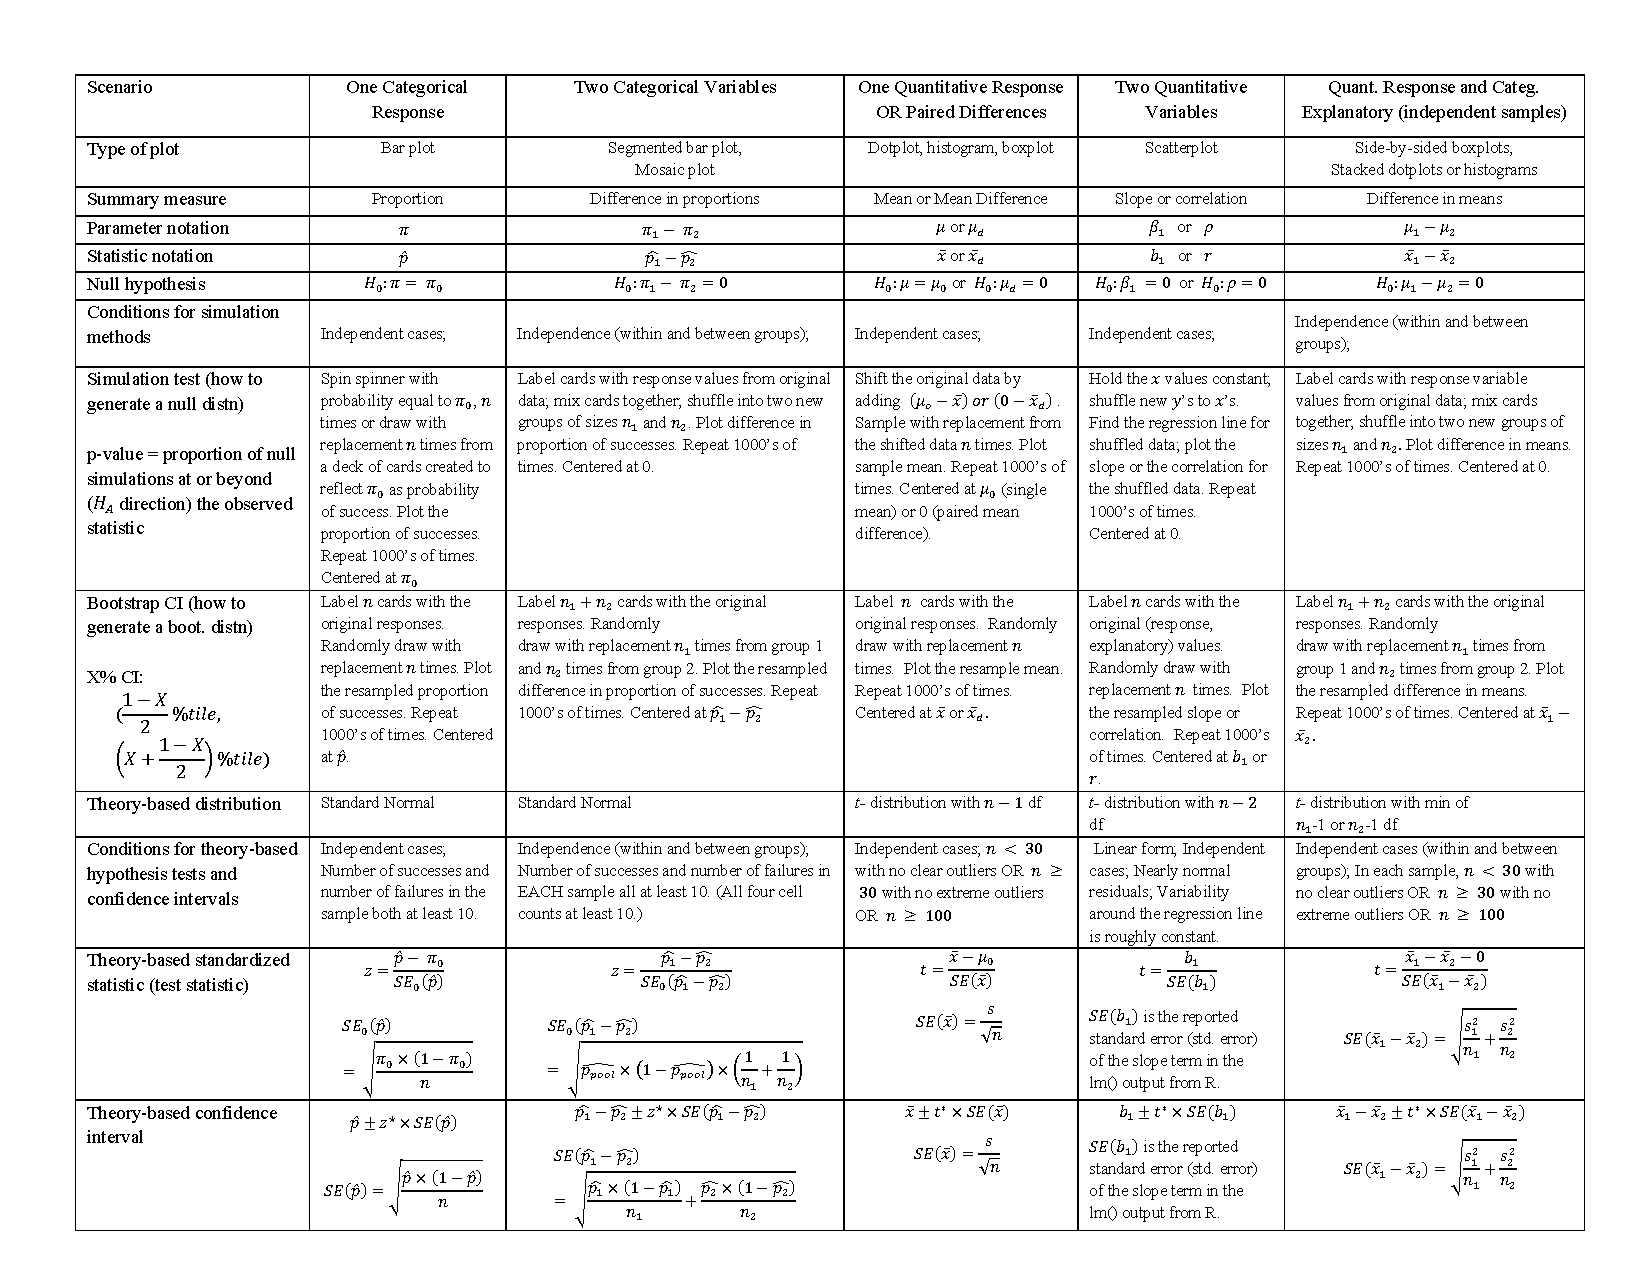
\includepdf[landscape=true]{GoldenTicket_F22.pdf}

\hypertarget{references}{%
\chapter*{References}\label{references}}
\addcontentsline{toc}{chapter}{References}

\hypertarget{refs}{}
\begin{CSLReferences}{1}{0}
\leavevmode\vadjust pre{\hypertarget{ref-pga}{}}%
{``Average Driving Distance and Fairway Accuracy.''} 2008. \href{https://www.pga.com/\%20and\%20https://www.lpga.com/}{https://www.pga.com/ and https://www.lpga.com/}.

\leavevmode\vadjust pre{\hypertarget{ref-islands}{}}%
Bulmer, M. n.d. {``Islands in Schools Project.''} \url{https://sites.google.com/site/islandsinschoolsprojectwebsite/home}.

\leavevmode\vadjust pre{\hypertarget{ref-darley1973}{}}%
Darley, J. M., and C. D. Batson. 1973. {``"From Jerusalem to Jericho": A Study of Situational and Dispositional Variables in Helping Behavior.''} \emph{Journal of Personality and Social Psychology} 27: 100--108.

\leavevmode\vadjust pre{\hypertarget{ref-ipeds}{}}%
Education Statistics, National Center for. 2018. {``IPEDS.''} \url{https://nces.ed.gov/ipeds/}.

\leavevmode\vadjust pre{\hypertarget{ref-zeitler2012}{}}%
Group, TODAY Study. 2012. {``\href{https://www.ncbi.nlm.nih.gov/pubmed/22540912}{A Clinical Trial to Maintain Glycemic Control in Youth with Type 2 Diabetes}.''} \emph{New England Journal of Medicine} 366: 2247--56.

\leavevmode\vadjust pre{\hypertarget{ref-hamblin2007}{}}%
Hamblin, J. K., K. Wynn, and P. Bloom. 2007. {``Social Evaluation by Preverbal Infants.''} \emph{Nature} 450 (6288): 557--59.

\leavevmode\vadjust pre{\hypertarget{ref-hirschfelder2018}{}}%
Hirschfelder, A., and P. F. Molin. 2018. {``I Is for Ignoble: Stereotyping Native Americans.''} \href{Retrieved\%20from\%20https://www.ferris.edu/HTMLS/news/jimcrow/native/homepage.htm.}{Retrieved from https://www.ferris.edu/HTMLS/news/jimcrow/native/homepage.htm.}

\leavevmode\vadjust pre{\hypertarget{ref-hutchison2013}{}}%
Hutchison, R. L., and M. A. Hirthler. 2013. {``\href{https://www.ncbi.nlm.nih.gov/pubmed/23932117}{Upper Extremity Injuies in Homer's Iliad}.''} \emph{Journal of Hand Surgery (American Volume)} 38: 1790--93.

\leavevmode\vadjust pre{\hypertarget{ref-imdb}{}}%
{``{IMDb} Movies Extensive Dataset.''} 2016. \url{https://kaggle.com/stefanoleone992/imdb-extensive-dataset}.

\leavevmode\vadjust pre{\hypertarget{ref-keating2021}{}}%
Keating, D., N. Ahmed, F. Nirappil, Stanley-Becker I., and L. Bernstein. 2021. {``Coronavirus Infections Dropping Where People Are Vaccinated, Rising Where They Are Not, Post Analysis Finds.''} \emph{Washington Post}. \url{https://www.washingtonpost.com/health/2021/06/14/covid-cases-vaccination-rates/}.

\leavevmode\vadjust pre{\hypertarget{ref-becentispeech}{}}%
Moquin, W., and C. Van Doren. 1973. {``Great Documents in American Indian History.''} Praeger.

\leavevmode\vadjust pre{\hypertarget{ref-weather}{}}%
National Weather Service Corporate Image Web Team. n.d. {``National Weather Service -- {NWS} Billings.''} \url{https://w2.weather.gov/climate/xmacis.php?wfo=byz}.

\leavevmode\vadjust pre{\hypertarget{ref-porath2017}{}}%
Porath, Erez, C. 2017. {``Does Rudeness Really Matter? The Effects of Rudeness on Task Performance and Helpfulness.''} \emph{Academy of Management Journal} 50.

\leavevmode\vadjust pre{\hypertarget{ref-quinn1999}{}}%
Quinn, G. E., C. H. Shin, M. G. Maguire, and R. A. Stone. 1999. {``Myopia and Ambient Lighting at Night.''} \emph{Nature} 399 (6732): 113--14. \url{https://doi.org/10.1038/20094}.

\leavevmode\vadjust pre{\hypertarget{ref-ramachandran2007}{}}%
Ramachandran, V. 2007. {``3 Clues to Understanding Your Brain.''} \url{https://www.ted.com/talks/vs_ramachandran_3_clues_to_understanding_your_brain}.

\leavevmode\vadjust pre{\hypertarget{ref-cdchospitalization}{}}%
{``Rates of Laboratory-Confimed COVID-19 Hospitalizations by Vaccination Status.''} 2021. CDC. \url{https://covid.cdc.gov/covid-data-tracker/\#covidnet-hospitalizations-vaccination}.

\leavevmode\vadjust pre{\hypertarget{ref-richardson2019}{}}%
Richardson, T., and R. T. Gilman. 2019. {``Left-Handedness Is Associated with Greater Fighting Success in Humans.''} \emph{Scientific Reports} 9 (1): 15402. \url{https://doi.org/10.1038/s41598-019-51975-3}.

\leavevmode\vadjust pre{\hypertarget{ref-stephens2020}{}}%
Stephens, R., and O. Robertson. 2020. {``Swearing as a Response to Pain: Assessing Hypoalgesic Effects of Novel "Swear" Words.''} \emph{Frontiers in Psychology} 11: 643--62.

\leavevmode\vadjust pre{\hypertarget{ref-stewart2014}{}}%
Stewart, E. H., B. Davis, B. L. Clemans-Taylor, B. Littenberg, C. A. Estrada, and R. M. Centor. 2014. {``Rapid Antigen Group a Streptococcus Test to Diagnose Pharyngitis: A Systematic Review and Meta-Analysis''} 9 (11). \url{https://doi.org/10.1371/journal.pone.0111727}.

\leavevmode\vadjust pre{\hypertarget{ref-stroop1935}{}}%
Stroop, J. R. 1935. {``Studies of Interference in Serial Verbal Reactions.''} \emph{Journal of Experimental Psychology} 18: 643--62.

\leavevmode\vadjust pre{\hypertarget{ref-sulheim2017}{}}%
Sulheim, S., A. Ekeland, I. Holme, and R. Bahr. 2017. {``Helmet Use and Risk of Head Injuries in Alpine Skiers and Snowboarders: Changes After an Interval of One Decade''} 51 (1): 44--50. \url{https://doi.org/10.1136/bjsports-2015-095798}.

\leavevmode\vadjust pre{\hypertarget{ref-titanic}{}}%
{``Titanic.''} n.d. \url{http://www.encyclopedia-titanica.org}.

\leavevmode\vadjust pre{\hypertarget{ref-covidvaccinetracker}{}}%
{``US COVID-19 Vaccine Tracker: See Your State's Progress.''} 2021. Mayo Clinic. \url{https://www.mayoclinic.org/coronavirus-covid-19/vaccine-tracker}.

\leavevmode\vadjust pre{\hypertarget{ref-usepa2020}{}}%
US Environmental Protection Agency. n.d. {``Air Data -- Daily Air Quality Tracker.''} \url{https://www.epa.gov/outdoor-air-quality-data/air-data-daily-air-quality-tracker}.

\leavevmode\vadjust pre{\hypertarget{ref-navajo2011}{}}%
{``Welcome to the Navajo Nation Government: Official Site of the Navajo Nation.''} 2011.\href{\%20Retrieved\%20from\%20https://www.navajo-nsn.gov/.}{Retrieved from https://www.navajo-nsn.gov/.}

\end{CSLReferences}

\end{document}
